\documentclass[twoside]{book}

% Packages required by doxygen
\usepackage{fixltx2e}
\usepackage{calc}
\usepackage{doxygen}
\usepackage[export]{adjustbox} % also loads graphicx
\usepackage{graphicx}
\usepackage[utf8]{inputenc}
\usepackage{makeidx}
\usepackage{multicol}
\usepackage{multirow}
\PassOptionsToPackage{warn}{textcomp}
\usepackage{textcomp}
\usepackage[nointegrals]{wasysym}
\usepackage[table]{xcolor}

% Font selection
\usepackage[T1]{fontenc}
\usepackage[scaled=.90]{helvet}
\usepackage{courier}
\usepackage{amssymb}
\usepackage{sectsty}
\renewcommand{\familydefault}{\sfdefault}
\allsectionsfont{%
  \fontseries{bc}\selectfont%
  \color{darkgray}%
}
\renewcommand{\DoxyLabelFont}{%
  \fontseries{bc}\selectfont%
  \color{darkgray}%
}
\newcommand{\+}{\discretionary{\mbox{\scriptsize$\hookleftarrow$}}{}{}}

% Page & text layout
\usepackage{geometry}
\geometry{%
  a4paper,%
  top=2.5cm,%
  bottom=2.5cm,%
  left=2.5cm,%
  right=2.5cm%
}
\tolerance=750
\hfuzz=15pt
\hbadness=750
\setlength{\emergencystretch}{15pt}
\setlength{\parindent}{0cm}
\setlength{\parskip}{3ex plus 2ex minus 2ex}
\makeatletter
\renewcommand{\paragraph}{%
  \@startsection{paragraph}{4}{0ex}{-1.0ex}{1.0ex}{%
    \normalfont\normalsize\bfseries\SS@parafont%
  }%
}
\renewcommand{\subparagraph}{%
  \@startsection{subparagraph}{5}{0ex}{-1.0ex}{1.0ex}{%
    \normalfont\normalsize\bfseries\SS@subparafont%
  }%
}
\makeatother

% Headers & footers
\usepackage{fancyhdr}
\pagestyle{fancyplain}
\fancyhead[LE]{\fancyplain{}{\bfseries\thepage}}
\fancyhead[CE]{\fancyplain{}{}}
\fancyhead[RE]{\fancyplain{}{\bfseries\leftmark}}
\fancyhead[LO]{\fancyplain{}{\bfseries\rightmark}}
\fancyhead[CO]{\fancyplain{}{}}
\fancyhead[RO]{\fancyplain{}{\bfseries\thepage}}
\fancyfoot[LE]{\fancyplain{}{}}
\fancyfoot[CE]{\fancyplain{}{}}
\fancyfoot[RE]{\fancyplain{}{\bfseries\scriptsize Generated by Doxygen }}
\fancyfoot[LO]{\fancyplain{}{\bfseries\scriptsize Generated by Doxygen }}
\fancyfoot[CO]{\fancyplain{}{}}
\fancyfoot[RO]{\fancyplain{}{}}
\renewcommand{\footrulewidth}{0.4pt}
\renewcommand{\chaptermark}[1]{%
  \markboth{#1}{}%
}
\renewcommand{\sectionmark}[1]{%
  \markright{\thesection\ #1}%
}

% Indices & bibliography
\usepackage{natbib}
\usepackage[titles]{tocloft}
\setcounter{tocdepth}{3}
\setcounter{secnumdepth}{5}
\makeindex

% Hyperlinks (required, but should be loaded last)
\usepackage{ifpdf}
\ifpdf
  \usepackage[pdftex,pagebackref=true]{hyperref}
\else
  \usepackage[ps2pdf,pagebackref=true]{hyperref}
\fi
\hypersetup{%
  colorlinks=true,%
  linkcolor=blue,%
  citecolor=blue,%
  unicode%
}

% Custom commands
\newcommand{\clearemptydoublepage}{%
  \newpage{\pagestyle{empty}\cleardoublepage}%
}

\usepackage{caption}
\captionsetup{labelsep=space,justification=centering,font={bf},singlelinecheck=off,skip=4pt,position=top}

%===== C O N T E N T S =====

\begin{document}

% Titlepage & ToC
\hypersetup{pageanchor=false,
             bookmarksnumbered=true,
             pdfencoding=unicode
            }
\pagenumbering{alph}
\begin{titlepage}
\vspace*{7cm}
\begin{center}%
{\Large S\+AC Effects \\[1ex]\large v1.\+0 }\\
\vspace*{1cm}
{\large Generated by Doxygen 1.8.13}\\
\end{center}
\end{titlepage}
\clearemptydoublepage
\pagenumbering{roman}
\tableofcontents
\clearemptydoublepage
\pagenumbering{arabic}
\hypersetup{pageanchor=true}

%--- Begin generated contents ---
\chapter{Namespace Index}
\section{Namespace List}
Here is a list of all namespaces with brief descriptions\+:\begin{DoxyCompactList}
\item\contentsline{section}{\textbf{ Ui} }{\pageref{namespace_ui}}{}
\end{DoxyCompactList}

\chapter{Hierarchical Index}
\section{Class Hierarchy}
This inheritance list is sorted roughly, but not completely, alphabetically\+:\begin{DoxyCompactList}
\item \contentsline{section}{Audio\+Signal}{\pageref{class_audio_signal}}{}
\item \contentsline{section}{Binaural\+Quality}{\pageref{struct_binaural_quality}}{}
\item \contentsline{section}{Channel}{\pageref{class_channel}}{}
\item \contentsline{section}{S\+A\+C\+Bitstream\+:\+:Channel\+Type}{\pageref{struct_s_a_c_bitstream_1_1_channel_type}}{}
\item \contentsline{section}{Chart2D\+:\+:Chart\+Options}{\pageref{struct_chart2_d_1_1_chart_options}}{}
\item \contentsline{section}{Compressor}{\pageref{class_compressor}}{}
\item \contentsline{section}{Decoding\+Type}{\pageref{struct_decoding_type}}{}
\item \contentsline{section}{Effect}{\pageref{class_effect}}{}
\item \contentsline{section}{Effect\+Base}{\pageref{class_effect_base}}{}
\item \contentsline{section}{File\+:\+:Endianess}{\pageref{struct_file_1_1_endianess}}{}
\item \contentsline{section}{Equalizer}{\pageref{class_equalizer}}{}
\item \contentsline{section}{File}{\pageref{class_file}}{}
\begin{DoxyCompactList}
\item \contentsline{section}{W\+A\+V\+File}{\pageref{class_w_a_v_file}}{}
\end{DoxyCompactList}
\item \contentsline{section}{W\+A\+V\+File\+:\+:Header}{\pageref{struct_w_a_v_file_1_1_header}}{}
\item \contentsline{section}{H\+R\+T\+F\+Model}{\pageref{struct_h_r_t_f_model}}{}
\item \contentsline{section}{Log\+Type}{\pageref{struct_log_type}}{}
\item \contentsline{section}{Panning}{\pageref{class_panning}}{}
\item \contentsline{section}{Process\+Manager}{\pageref{class_process_manager}}{}
\item Q\+Dialog\begin{DoxyCompactList}
\item \contentsline{section}{Audio\+Info}{\pageref{class_audio_info}}{}
\item \contentsline{section}{Audio\+Test}{\pageref{class_audio_test}}{}
\item \contentsline{section}{Channels\+Charts}{\pageref{class_channels_charts}}{}
\item \contentsline{section}{Encoder}{\pageref{class_encoder}}{}
\end{DoxyCompactList}
\item Q\+I\+O\+Device\begin{DoxyCompactList}
\item \contentsline{section}{Output\+Device}{\pageref{class_output_device}}{}
\end{DoxyCompactList}
\item Q\+Main\+Window\begin{DoxyCompactList}
\item \contentsline{section}{S\+A\+C\+Effects}{\pageref{class_s_a_c_effects}}{}
\end{DoxyCompactList}
\item Q\+Object\begin{DoxyCompactList}
\item \contentsline{section}{Audio\+Output}{\pageref{class_audio_output}}{}
\item \contentsline{section}{Channels\+List}{\pageref{class_channels_list}}{}
\item \contentsline{section}{Effects\+Monitor}{\pageref{class_effects_monitor}}{}
\end{DoxyCompactList}
\item Q\+Widget\begin{DoxyCompactList}
\item \contentsline{section}{Chart2D}{\pageref{class_chart2_d}}{}
\end{DoxyCompactList}
\item \contentsline{section}{Reverb}{\pageref{class_reverb}}{}
\item \contentsline{section}{S\+A\+C\+Bitstream}{\pageref{class_s_a_c_bitstream}}{}
\item \contentsline{section}{Upmix\+Type}{\pageref{struct_upmix_type}}{}
\end{DoxyCompactList}

\chapter{Class Index}
\section{Class List}
Here are the classes, structs, unions and interfaces with brief descriptions\+:\begin{DoxyCompactList}
\item\contentsline{section}{\textbf{ A\+S\+\_\+\+E\+F\+F\+E\+CT} }{\pageref{class_a_s___e_f_f_e_c_t}}{}
\item\contentsline{section}{\textbf{ Audio\+Info} \\*Audio object info dialog class }{\pageref{class_audio_info}}{}
\item\contentsline{section}{\textbf{ Audio\+Output} \\*Audio output class }{\pageref{class_audio_output}}{}
\item\contentsline{section}{\textbf{ Audio\+Signal} \\*Audio signal class }{\pageref{class_audio_signal}}{}
\item\contentsline{section}{\textbf{ Audio\+Stream} \\*Audio objects for the S\+A\+OC interface }{\pageref{class_audio_stream}}{}
\item\contentsline{section}{\textbf{ Audio\+Test} \\*Audio output test class }{\pageref{class_audio_test}}{}
\item\contentsline{section}{\textbf{ Binaural\+Quality} \\*S\+AC decoder parameter binaural quality }{\pageref{struct_binaural_quality}}{}
\item\contentsline{section}{\textbf{ Channel} \\*Single-\/object class from channels list }{\pageref{class_channel}}{}
\item\contentsline{section}{\textbf{ Channels\+Charts} }{\pageref{class_channels_charts}}{}
\item\contentsline{section}{\textbf{ Channels\+List} \\*Channels list class. It shows information about channels signals }{\pageref{class_channels_list}}{}
\item\contentsline{section}{\textbf{ S\+A\+C\+Bitstream\+::\+Channel\+Type} \\*It specifies the channel type }{\pageref{struct_s_a_c_bitstream_1_1_channel_type}}{}
\item\contentsline{section}{\textbf{ Chart2D} \\*Class for plotting two-\/dimensional charts }{\pageref{class_chart2_d}}{}
\item\contentsline{section}{\textbf{ Chart2\+D\+::\+Chart\+Options} \\*It defines some features of the chart }{\pageref{struct_chart2_d_1_1_chart_options}}{}
\item\contentsline{section}{\textbf{ Compressor} \\*Audio compressor }{\pageref{class_compressor}}{}
\item\contentsline{section}{\textbf{ Decoding\+Type} \\*S\+AC decoder parameter decoding type }{\pageref{struct_decoding_type}}{}
\item\contentsline{section}{\textbf{ Effect} \\*\doxyref{Effect}{p.}{class_effect} class. It contains (by inheritance) all effects classes }{\pageref{class_effect}}{}
\item\contentsline{section}{\textbf{ Effect\+Base} \\*\doxyref{Effect}{p.}{class_effect} base class }{\pageref{class_effect_base}}{}
\item\contentsline{section}{\textbf{ Effects\+Monitor} \\*Class for managing effects parameters }{\pageref{class_effects_monitor}}{}
\item\contentsline{section}{\textbf{ Encoder} \\*\doxyref{Encoder}{p.}{class_encoder} window interface }{\pageref{class_encoder}}{}
\item\contentsline{section}{\textbf{ File\+::\+Endianess} }{\pageref{struct_file_1_1_endianess}}{}
\item\contentsline{section}{\textbf{ Equalizer} \\*Audio compressor }{\pageref{class_equalizer}}{}
\item\contentsline{section}{\textbf{ File} \\*Audio file class }{\pageref{class_file}}{}
\item\contentsline{section}{\textbf{ W\+A\+V\+File\+::\+Header} \\*Audio file header struct }{\pageref{struct_w_a_v_file_1_1_header}}{}
\item\contentsline{section}{\textbf{ H\+R\+T\+F\+Model} \\*S\+AC decoder parameter H\+R\+TF model }{\pageref{struct_h_r_t_f_model}}{}
\item\contentsline{section}{\textbf{ Log\+Type} }{\pageref{struct_log_type}}{}
\item\contentsline{section}{\textbf{ Output\+Device} \\*Audio output device class (Q\+I\+O\+Device extension) }{\pageref{class_output_device}}{}
\item\contentsline{section}{\textbf{ Process\+Manager} \\*Process manager class. It contains all functions to perform the signal treatment process }{\pageref{class_process_manager}}{}
\item\contentsline{section}{\textbf{ Reverb} \\*Audio reverb effect }{\pageref{class_reverb}}{}
\item\contentsline{section}{\textbf{ S\+A\+C\+Bitstream} \\*S\+AC bitstream class }{\pageref{class_s_a_c_bitstream}}{}
\item\contentsline{section}{\textbf{ S\+A\+C\+Effects} \\*\doxyref{S\+A\+C\+Effects}{p.}{class_s_a_c_effects} window interface }{\pageref{class_s_a_c_effects}}{}
\item\contentsline{section}{\textbf{ Audio\+Stream\+::\+Time\+Slot} \\*It indicates time slot of the available signal }{\pageref{struct_audio_stream_1_1_time_slot}}{}
\item\contentsline{section}{\textbf{ Upmix\+Type} \\*S\+AC decoder parameter upmix type }{\pageref{struct_upmix_type}}{}
\item\contentsline{section}{\textbf{ W\+A\+V\+File} \\*Audio file as W\+AV format class }{\pageref{class_w_a_v_file}}{}
\end{DoxyCompactList}

\chapter{File Index}
\section{File List}
Here is a list of all documented files with brief descriptions\+:\begin{DoxyCompactList}
\item\contentsline{section}{src/{\bfseries main.\+cpp} }{\pageref{main_8cpp}}{}
\item\contentsline{section}{src/effects/{\bfseries Compressor.\+cpp} }{\pageref{_compressor_8cpp}}{}
\item\contentsline{section}{src/effects/{\bfseries Compressor.\+h} }{\pageref{_compressor_8h}}{}
\item\contentsline{section}{src/effects/{\bfseries Effect.\+cpp} }{\pageref{_effect_8cpp}}{}
\item\contentsline{section}{src/effects/{\bfseries Effect.\+h} }{\pageref{_effect_8h}}{}
\item\contentsline{section}{src/effects/{\bfseries Effect\+Base.\+h} }{\pageref{_effect_base_8h}}{}
\item\contentsline{section}{src/effects/{\bfseries Equalizer.\+cpp} }{\pageref{_equalizer_8cpp}}{}
\item\contentsline{section}{src/effects/{\bfseries Equalizer.\+h} }{\pageref{_equalizer_8h}}{}
\item\contentsline{section}{src/effects/{\bfseries Panning.\+cpp} }{\pageref{_panning_8cpp}}{}
\item\contentsline{section}{src/effects/{\bfseries Panning.\+h} }{\pageref{_panning_8h}}{}
\item\contentsline{section}{src/effects/{\bfseries Reverb.\+cpp} }{\pageref{_reverb_8cpp}}{}
\item\contentsline{section}{src/effects/{\bfseries Reverb.\+h} }{\pageref{_reverb_8h}}{}
\item\contentsline{section}{src/interface/{\bfseries Audio\+Info.\+cpp} }{\pageref{_audio_info_8cpp}}{}
\item\contentsline{section}{src/interface/{\bfseries Audio\+Info.\+h} }{\pageref{_audio_info_8h}}{}
\item\contentsline{section}{src/interface/{\bfseries Audio\+Output.\+cpp} }{\pageref{_audio_output_8cpp}}{}
\item\contentsline{section}{src/interface/{\bfseries Audio\+Output.\+h} }{\pageref{_audio_output_8h}}{}
\item\contentsline{section}{src/interface/{\bfseries Channels\+List.\+cpp} }{\pageref{_channels_list_8cpp}}{}
\item\contentsline{section}{src/interface/{\bfseries Channels\+List.\+h} }{\pageref{_channels_list_8h}}{}
\item\contentsline{section}{src/interface/{\bfseries Chart2\+D.\+cpp} }{\pageref{_chart2_d_8cpp}}{}
\item\contentsline{section}{src/interface/{\bfseries Chart2\+D.\+h} }{\pageref{_chart2_d_8h}}{}
\item\contentsline{section}{src/interface/{\bfseries Effects\+Monitor.\+cpp} }{\pageref{_effects_monitor_8cpp}}{}
\item\contentsline{section}{src/interface/{\bfseries Effects\+Monitor.\+h} }{\pageref{_effects_monitor_8h}}{}
\item\contentsline{section}{src/interface/{\bfseries Encoder.\+cpp} }{\pageref{_encoder_8cpp}}{}
\item\contentsline{section}{src/interface/{\bfseries Encoder.\+h} }{\pageref{_encoder_8h}}{}
\item\contentsline{section}{src/interface/{\bfseries main.\+cpp} }{\pageref{interface_2main_8cpp}}{}
\item\contentsline{section}{src/interface/{\bfseries S\+A\+C\+Effects.\+cpp} }{\pageref{_s_a_c_effects_8cpp}}{}
\item\contentsline{section}{src/interface/{\bfseries S\+A\+C\+Effects.\+h} }{\pageref{_s_a_c_effects_8h}}{}
\item\contentsline{section}{src/process/{\bfseries Audio\+Signal.\+cpp} }{\pageref{_audio_signal_8cpp}}{}
\item\contentsline{section}{src/process/{\bfseries Audio\+Signal.\+h} }{\pageref{_audio_signal_8h}}{}
\item\contentsline{section}{src/process/{\bfseries File.\+cpp} }{\pageref{_file_8cpp}}{}
\item\contentsline{section}{src/process/{\bfseries File.\+h} }{\pageref{_file_8h}}{}
\item\contentsline{section}{src/process/{\bfseries Process\+Manager.\+cpp} }{\pageref{_process_manager_8cpp}}{}
\item\contentsline{section}{src/process/{\bfseries Process\+Manager.\+h} }{\pageref{_process_manager_8h}}{}
\item\contentsline{section}{src/sac/{\bfseries sac\+\_\+decoder.\+c} }{\pageref{sac__decoder_8c}}{}
\item\contentsline{section}{src/sac/{\bfseries sac\+\_\+decoder.\+h} }{\pageref{sac__decoder_8h}}{}
\item\contentsline{section}{src/sac/{\bfseries sac\+\_\+encoder.\+c} }{\pageref{sac__encoder_8c}}{}
\item\contentsline{section}{src/sac/{\bfseries sac\+\_\+encoder.\+h} }{\pageref{sac__encoder_8h}}{}
\item\contentsline{section}{src/sac/{\bfseries S\+A\+C\+Bitstream.\+cpp} }{\pageref{_s_a_c_bitstream_8cpp}}{}
\item\contentsline{section}{src/sac/{\bfseries S\+A\+C\+Bitstream.\+h} }{\pageref{_s_a_c_bitstream_8h}}{}
\item\contentsline{section}{src/tools/\hyperlink{_logger_8cpp}{Logger.\+cpp} \\*Functions to create log messages on console }{\pageref{_logger_8cpp}}{}
\item\contentsline{section}{src/tools/{\bfseries Logger.\+h} }{\pageref{_logger_8h}}{}
\end{DoxyCompactList}

\chapter{Namespace Documentation}
\section{Ui Namespace Reference}
\label{namespace_ui}\index{Ui@{Ui}}

\chapter{Class Documentation}
\section{Audio\+Info Class Reference}
\label{class_audio_info}\index{Audio\+Info@{Audio\+Info}}


Audio object info dialog class.  




{\ttfamily \#include $<$Audio\+Info.\+h$>$}

Inheritance diagram for Audio\+Info\+:\begin{figure}[H]
\begin{center}
\leavevmode
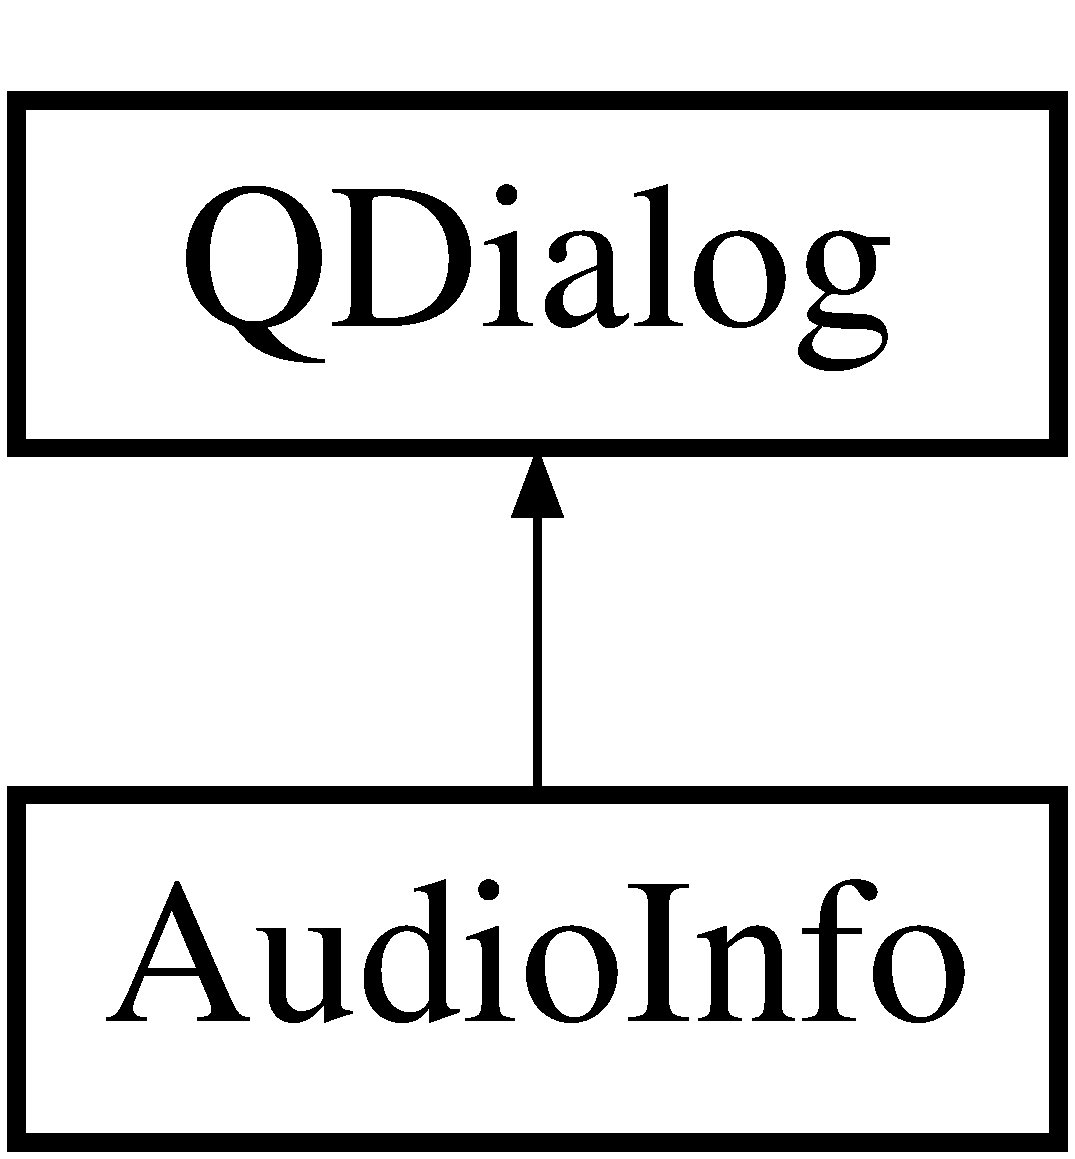
\includegraphics[height=2.000000cm]{class_audio_info}
\end{center}
\end{figure}
\subsection*{Public Member Functions}
\begin{DoxyCompactItemize}
\item 
\textbf{ Audio\+Info} (Q\+Widget $\ast$parent=0)
\begin{DoxyCompactList}\small\item\em \doxyref{Audio\+Info}{p.}{class_audio_info} constructor. \end{DoxyCompactList}\item 
\textbf{ $\sim$\+Audio\+Info} ()
\begin{DoxyCompactList}\small\item\em \doxyref{Audio\+Info}{p.}{class_audio_info} destructor. \end{DoxyCompactList}\item 
void \textbf{ set\+File} (\textbf{ W\+A\+V\+File} $\ast$\textbf{ file})
\begin{DoxyCompactList}\small\item\em It sets a audio file. \end{DoxyCompactList}\end{DoxyCompactItemize}
\subsection*{Private Attributes}
\begin{DoxyCompactItemize}
\item 
Ui\+::\+Audio\+Info $\ast$ \textbf{ ui}
\item 
\textbf{ W\+A\+V\+File} $\ast$ \textbf{ file}
\end{DoxyCompactItemize}


\subsection{Detailed Description}
Audio object info dialog class. 

\begin{DoxyAuthor}{Author}
Andrés González Fornell 
\end{DoxyAuthor}


\subsection{Constructor \& Destructor Documentation}
\mbox{\label{class_audio_info_ad24c69ecc331c48790cdf2886c721132}} 
\index{Audio\+Info@{Audio\+Info}!Audio\+Info@{Audio\+Info}}
\index{Audio\+Info@{Audio\+Info}!Audio\+Info@{Audio\+Info}}
\subsubsection{Audio\+Info()}
{\footnotesize\ttfamily Audio\+Info\+::\+Audio\+Info (\begin{DoxyParamCaption}\item[{Q\+Widget $\ast$}]{parent = {\ttfamily 0} }\end{DoxyParamCaption})}



\doxyref{Audio\+Info}{p.}{class_audio_info} constructor. 


\begin{DoxyParams}{Parameters}
{\em parent} & user interface parent object \\
\hline
\end{DoxyParams}
\mbox{\label{class_audio_info_ae6b316306b98617ceda7624bb04138fd}} 
\index{Audio\+Info@{Audio\+Info}!````~Audio\+Info@{$\sim$\+Audio\+Info}}
\index{````~Audio\+Info@{$\sim$\+Audio\+Info}!Audio\+Info@{Audio\+Info}}
\subsubsection{$\sim$\+Audio\+Info()}
{\footnotesize\ttfamily Audio\+Info\+::$\sim$\+Audio\+Info (\begin{DoxyParamCaption}{ }\end{DoxyParamCaption})}



\doxyref{Audio\+Info}{p.}{class_audio_info} destructor. 



\subsection{Member Function Documentation}
\mbox{\label{class_audio_info_a2d05a12b4191202227e17afc5e57f349}} 
\index{Audio\+Info@{Audio\+Info}!set\+File@{set\+File}}
\index{set\+File@{set\+File}!Audio\+Info@{Audio\+Info}}
\subsubsection{set\+File()}
{\footnotesize\ttfamily void Audio\+Info\+::set\+File (\begin{DoxyParamCaption}\item[{\textbf{ W\+A\+V\+File} $\ast$}]{file }\end{DoxyParamCaption})}



It sets a audio file. 


\begin{DoxyParams}{Parameters}
{\em file} & audio file object \\
\hline
\end{DoxyParams}


\subsection{Member Data Documentation}
\mbox{\label{class_audio_info_a6bca5500a5f697ae90e0c6ed12efad90}} 
\index{Audio\+Info@{Audio\+Info}!file@{file}}
\index{file@{file}!Audio\+Info@{Audio\+Info}}
\subsubsection{file}
{\footnotesize\ttfamily \textbf{ W\+A\+V\+File}$\ast$ Audio\+Info\+::file\hspace{0.3cm}{\ttfamily [private]}}

audio file object \mbox{\label{class_audio_info_a44a21dbc93b654da1ef6de938372fdfb}} 
\index{Audio\+Info@{Audio\+Info}!ui@{ui}}
\index{ui@{ui}!Audio\+Info@{Audio\+Info}}
\subsubsection{ui}
{\footnotesize\ttfamily Ui\+::\+Audio\+Info$\ast$ Audio\+Info\+::ui\hspace{0.3cm}{\ttfamily [private]}}

user interface object 

The documentation for this class was generated from the following files\+:\begin{DoxyCompactItemize}
\item 
src/interface/\textbf{ Audio\+Info.\+h}\item 
src/interface/\textbf{ Audio\+Info.\+cpp}\end{DoxyCompactItemize}

\hypertarget{class_audio_output}{}\section{Audio\+Output Class Reference}
\label{class_audio_output}\index{Audio\+Output@{Audio\+Output}}


Audio output class.  




{\ttfamily \#include $<$Audio\+Output.\+h$>$}



Inheritance diagram for Audio\+Output\+:
\nopagebreak
\begin{figure}[H]
\begin{center}
\leavevmode
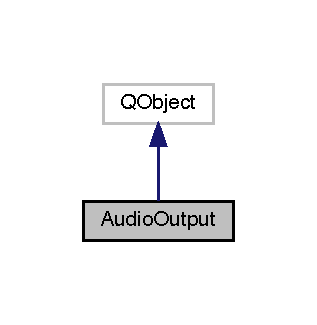
\includegraphics[width=152pt]{class_audio_output__inherit__graph}
\end{center}
\end{figure}


Collaboration diagram for Audio\+Output\+:
\nopagebreak
\begin{figure}[H]
\begin{center}
\leavevmode
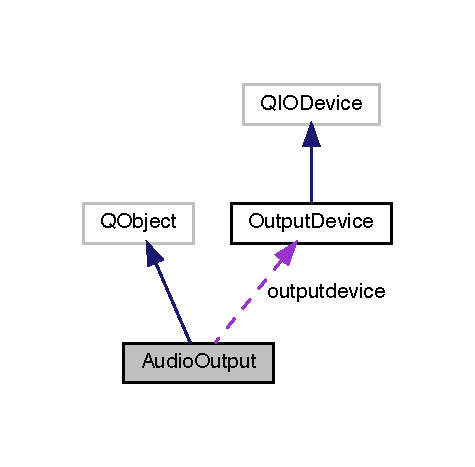
\includegraphics[width=228pt]{class_audio_output__coll__graph}
\end{center}
\end{figure}
\subsection*{Public Slots}
\begin{Indent}\textbf{ User interface slots}\par
{\em They are called when a user interface element is being changed. }\begin{DoxyCompactItemize}
\item 
void \hyperlink{class_audio_output_a1bfc3c2ca0fa53a8e2962ef784014317}{set\+Device} (int index)
\begin{DoxyCompactList}\small\item\em It selects an output device. \end{DoxyCompactList}\end{DoxyCompactItemize}
\end{Indent}
\subsection*{Public Member Functions}
\begin{DoxyCompactItemize}
\item 
\hyperlink{class_audio_output_afd879db4e79ccc430bd9d9a795534323}{Audio\+Output} (Q\+Combo\+Box $\ast$selector, int \hyperlink{class_audio_output_ac2a46ded8a978627b8af81458a714ef3}{fs}, int \hyperlink{class_audio_output_aac9c297a839bb25c1232fc5adcce6cab}{samplesize})
\begin{DoxyCompactList}\small\item\em Audio\+Ouput constructor. \end{DoxyCompactList}\item 
\mbox{\Hypertarget{class_audio_output_a95719dfdce3899ee2847e20dc403e25e}\label{class_audio_output_a95719dfdce3899ee2847e20dc403e25e}} 
\hyperlink{class_audio_output_a95719dfdce3899ee2847e20dc403e25e}{$\sim$\+Audio\+Output} ()
\begin{DoxyCompactList}\small\item\em \hyperlink{class_audio_output}{Audio\+Output} destructor. \end{DoxyCompactList}\item 
\mbox{\Hypertarget{class_audio_output_a686dd972cb2043552063b34ae67eaadc}\label{class_audio_output_a686dd972cb2043552063b34ae67eaadc}} 
void \hyperlink{class_audio_output_a686dd972cb2043552063b34ae67eaadc}{start} ()
\begin{DoxyCompactList}\small\item\em It resumes audio output playback. \end{DoxyCompactList}\item 
\mbox{\Hypertarget{class_audio_output_a3f4858aa5c581613e32b30ee6c5339a6}\label{class_audio_output_a3f4858aa5c581613e32b30ee6c5339a6}} 
void \hyperlink{class_audio_output_a3f4858aa5c581613e32b30ee6c5339a6}{stop} ()
\begin{DoxyCompactList}\small\item\em It stops audio output playback. \end{DoxyCompactList}\item 
void \hyperlink{class_audio_output_a467f6e31cf89b89e9986caa05ec7fe62}{set\+Format} (int \hyperlink{class_audio_output_ac2a46ded8a978627b8af81458a714ef3}{fs}, int \hyperlink{class_audio_output_aac9c297a839bb25c1232fc5adcce6cab}{samplesize})
\begin{DoxyCompactList}\small\item\em It sets signal sampling frequency. \end{DoxyCompactList}\item 
\mbox{\Hypertarget{class_audio_output_a5b8fb2dfc8057c8195c192ae65820821}\label{class_audio_output_a5b8fb2dfc8057c8195c192ae65820821}} 
void \hyperlink{class_audio_output_a5b8fb2dfc8057c8195c192ae65820821}{set\+Devices} ()
\begin{DoxyCompactList}\small\item\em It sets all available audio output devices. \end{DoxyCompactList}\item 
void \hyperlink{class_audio_output_a27ada29ff74a99f5c21d949caba261ee}{set\+Devices} (Q\+List$<$ Q\+Audio\+Device\+Info $>$ devices)
\begin{DoxyCompactList}\small\item\em It sets a list of audio devices. \end{DoxyCompactList}\item 
void \hyperlink{class_audio_output_a97008d6a17c3dc03c64e421f563e04b8}{set\+Volume} (float \hyperlink{class_audio_output_a16937c9086904959b06b77326032aa72}{volume})
\begin{DoxyCompactList}\small\item\em It sets audio output volume level. \end{DoxyCompactList}\end{DoxyCompactItemize}
\subsection*{Public Attributes}
\begin{DoxyCompactItemize}
\item 
\hyperlink{class_output_device}{Output\+Device} $\ast$ \hyperlink{class_audio_output_aa3e000199604f972e59242fb15a6707e}{outputdevice}
\item 
int \hyperlink{class_audio_output_ac2a46ded8a978627b8af81458a714ef3}{fs}
\item 
int \hyperlink{class_audio_output_aac9c297a839bb25c1232fc5adcce6cab}{samplesize}
\item 
float \hyperlink{class_audio_output_a16937c9086904959b06b77326032aa72}{volume}
\end{DoxyCompactItemize}


\subsection{Detailed Description}
\begin{DoxyAuthor}{Author}
Andrés González Fornell 
\end{DoxyAuthor}


Definition at line 58 of file Audio\+Output.\+h.



\subsection{Constructor \& Destructor Documentation}
\mbox{\Hypertarget{class_audio_output_afd879db4e79ccc430bd9d9a795534323}\label{class_audio_output_afd879db4e79ccc430bd9d9a795534323}} 
\index{Audio\+Output@{Audio\+Output}!Audio\+Output@{Audio\+Output}}
\index{Audio\+Output@{Audio\+Output}!Audio\+Output@{Audio\+Output}}
\subsubsection{\texorpdfstring{Audio\+Output()}{AudioOutput()}}
{\footnotesize\ttfamily Audio\+Output\+::\+Audio\+Output (\begin{DoxyParamCaption}\item[{Q\+Combo\+Box $\ast$}]{selector,  }\item[{int}]{fs,  }\item[{int}]{samplesize }\end{DoxyParamCaption})}


\begin{DoxyParams}{Parameters}
{\em selector} & user interface combo box to select audio device \\
\hline
{\em fs} & signal sampling frequency \\
\hline
{\em samplesize} & audio sample size \mbox{[}bits\mbox{]} \\
\hline
\end{DoxyParams}


Definition at line 10 of file Audio\+Output.\+cpp.

Here is the call graph for this function\+:
\nopagebreak
\begin{figure}[H]
\begin{center}
\leavevmode
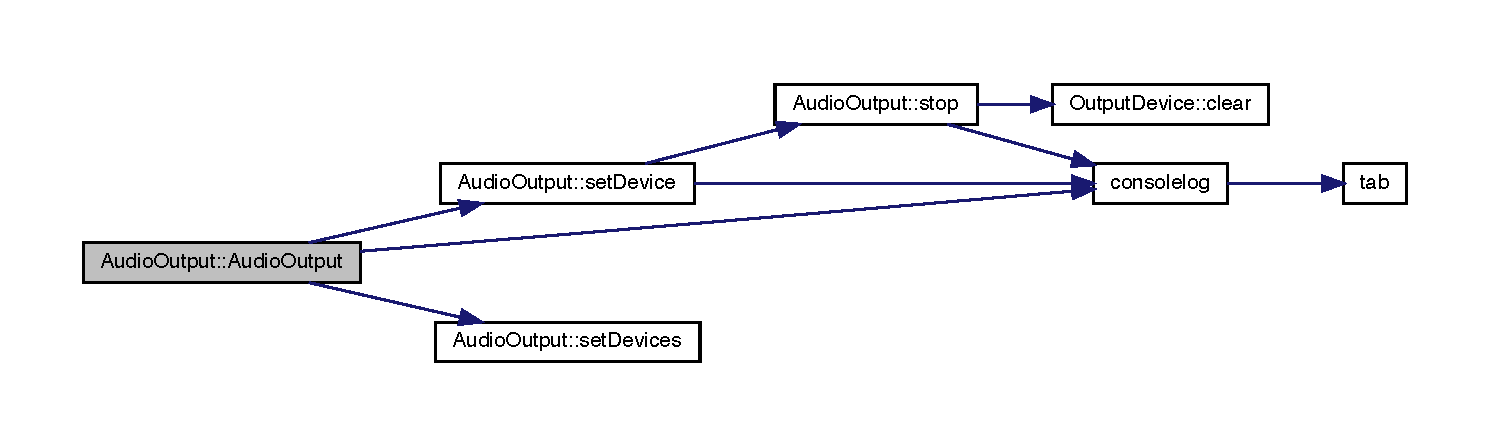
\includegraphics[width=350pt]{class_audio_output_afd879db4e79ccc430bd9d9a795534323_cgraph}
\end{center}
\end{figure}


\subsection{Member Function Documentation}
\mbox{\Hypertarget{class_audio_output_a1bfc3c2ca0fa53a8e2962ef784014317}\label{class_audio_output_a1bfc3c2ca0fa53a8e2962ef784014317}} 
\index{Audio\+Output@{Audio\+Output}!set\+Device@{set\+Device}}
\index{set\+Device@{set\+Device}!Audio\+Output@{Audio\+Output}}
\subsubsection{\texorpdfstring{set\+Device}{setDevice}}
{\footnotesize\ttfamily void Audio\+Output\+::set\+Device (\begin{DoxyParamCaption}\item[{int}]{index }\end{DoxyParamCaption})\hspace{0.3cm}{\ttfamily [slot]}}


\begin{DoxyParams}{Parameters}
{\em index} & device index \\
\hline
\end{DoxyParams}


Definition at line 137 of file Audio\+Output.\+cpp.

Here is the call graph for this function\+:
\nopagebreak
\begin{figure}[H]
\begin{center}
\leavevmode
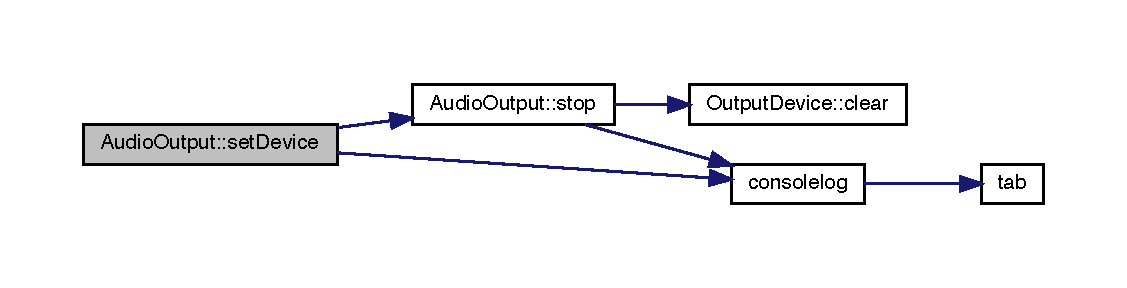
\includegraphics[width=350pt]{class_audio_output_a1bfc3c2ca0fa53a8e2962ef784014317_cgraph}
\end{center}
\end{figure}
Here is the caller graph for this function\+:
\nopagebreak
\begin{figure}[H]
\begin{center}
\leavevmode
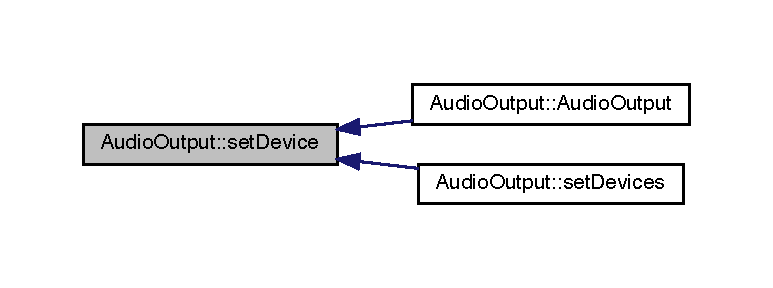
\includegraphics[width=350pt]{class_audio_output_a1bfc3c2ca0fa53a8e2962ef784014317_icgraph}
\end{center}
\end{figure}
\mbox{\Hypertarget{class_audio_output_a27ada29ff74a99f5c21d949caba261ee}\label{class_audio_output_a27ada29ff74a99f5c21d949caba261ee}} 
\index{Audio\+Output@{Audio\+Output}!set\+Devices@{set\+Devices}}
\index{set\+Devices@{set\+Devices}!Audio\+Output@{Audio\+Output}}
\subsubsection{\texorpdfstring{set\+Devices()}{setDevices()}}
{\footnotesize\ttfamily void Audio\+Output\+::set\+Devices (\begin{DoxyParamCaption}\item[{Q\+List$<$ Q\+Audio\+Device\+Info $>$}]{devices }\end{DoxyParamCaption})}


\begin{DoxyParams}{Parameters}
{\em devices} & \\
\hline
\end{DoxyParams}


Definition at line 100 of file Audio\+Output.\+cpp.

Here is the call graph for this function\+:
\nopagebreak
\begin{figure}[H]
\begin{center}
\leavevmode
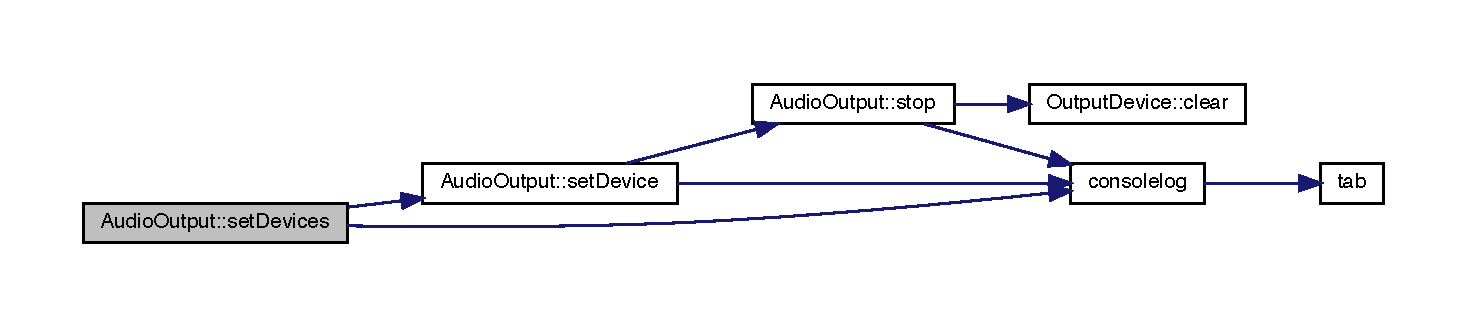
\includegraphics[width=350pt]{class_audio_output_a27ada29ff74a99f5c21d949caba261ee_cgraph}
\end{center}
\end{figure}
\mbox{\Hypertarget{class_audio_output_a467f6e31cf89b89e9986caa05ec7fe62}\label{class_audio_output_a467f6e31cf89b89e9986caa05ec7fe62}} 
\index{Audio\+Output@{Audio\+Output}!set\+Format@{set\+Format}}
\index{set\+Format@{set\+Format}!Audio\+Output@{Audio\+Output}}
\subsubsection{\texorpdfstring{set\+Format()}{setFormat()}}
{\footnotesize\ttfamily void Audio\+Output\+::set\+Format (\begin{DoxyParamCaption}\item[{int}]{fs,  }\item[{int}]{samplesize }\end{DoxyParamCaption})}


\begin{DoxyParams}{Parameters}
{\em fs} & signal sampling frequency. \\
\hline
{\em samplesize} & signal sample size \\
\hline
\end{DoxyParams}


Definition at line 83 of file Audio\+Output.\+cpp.

Here is the caller graph for this function\+:
\nopagebreak
\begin{figure}[H]
\begin{center}
\leavevmode
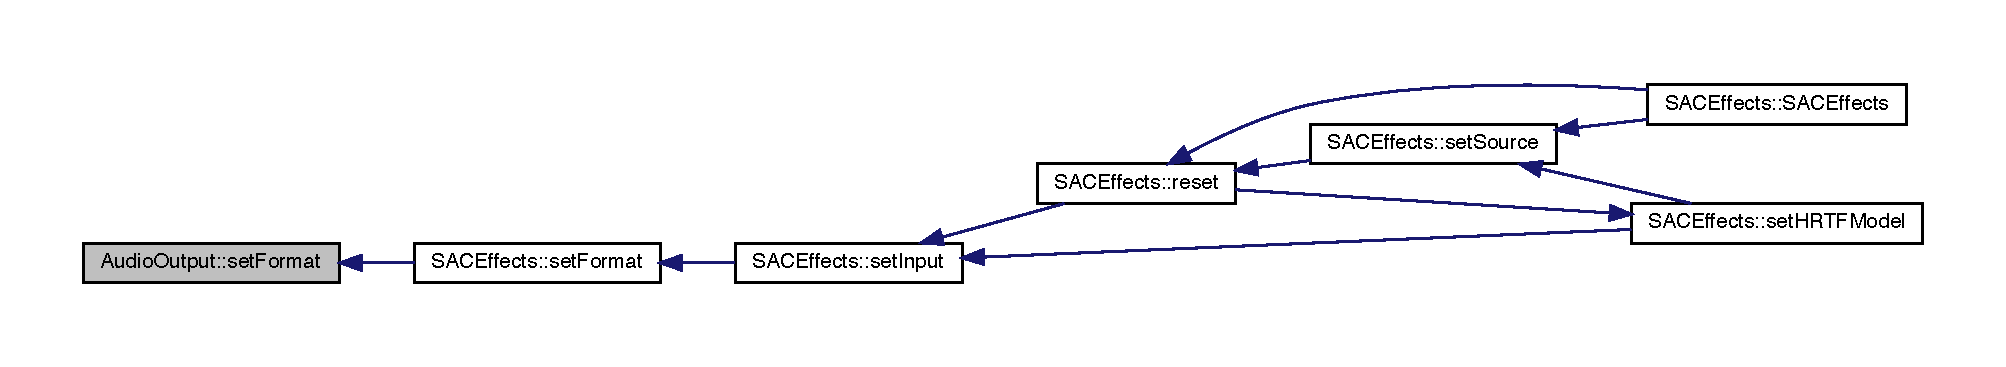
\includegraphics[width=350pt]{class_audio_output_a467f6e31cf89b89e9986caa05ec7fe62_icgraph}
\end{center}
\end{figure}
\mbox{\Hypertarget{class_audio_output_a97008d6a17c3dc03c64e421f563e04b8}\label{class_audio_output_a97008d6a17c3dc03c64e421f563e04b8}} 
\index{Audio\+Output@{Audio\+Output}!set\+Volume@{set\+Volume}}
\index{set\+Volume@{set\+Volume}!Audio\+Output@{Audio\+Output}}
\subsubsection{\texorpdfstring{set\+Volume()}{setVolume()}}
{\footnotesize\ttfamily void Audio\+Output\+::set\+Volume (\begin{DoxyParamCaption}\item[{float}]{volume }\end{DoxyParamCaption})}


\begin{DoxyParams}{Parameters}
{\em volume} & real number from 0 to 1 \\
\hline
\end{DoxyParams}


Definition at line 122 of file Audio\+Output.\+cpp.



\subsection{Member Data Documentation}
\mbox{\Hypertarget{class_audio_output_ac2a46ded8a978627b8af81458a714ef3}\label{class_audio_output_ac2a46ded8a978627b8af81458a714ef3}} 
\index{Audio\+Output@{Audio\+Output}!fs@{fs}}
\index{fs@{fs}!Audio\+Output@{Audio\+Output}}
\subsubsection{\texorpdfstring{fs}{fs}}
{\footnotesize\ttfamily int Audio\+Output\+::fs}

signal sampling frequency \mbox{[}Hz\mbox{]} 

Definition at line 62 of file Audio\+Output.\+h.

\mbox{\Hypertarget{class_audio_output_aa3e000199604f972e59242fb15a6707e}\label{class_audio_output_aa3e000199604f972e59242fb15a6707e}} 
\index{Audio\+Output@{Audio\+Output}!outputdevice@{outputdevice}}
\index{outputdevice@{outputdevice}!Audio\+Output@{Audio\+Output}}
\subsubsection{\texorpdfstring{outputdevice}{outputdevice}}
{\footnotesize\ttfamily \hyperlink{class_output_device}{Output\+Device}$\ast$ Audio\+Output\+::outputdevice}

audio output Q\+I\+O\+Device class object to control audio output device functions 

Definition at line 61 of file Audio\+Output.\+h.

\mbox{\Hypertarget{class_audio_output_aac9c297a839bb25c1232fc5adcce6cab}\label{class_audio_output_aac9c297a839bb25c1232fc5adcce6cab}} 
\index{Audio\+Output@{Audio\+Output}!samplesize@{samplesize}}
\index{samplesize@{samplesize}!Audio\+Output@{Audio\+Output}}
\subsubsection{\texorpdfstring{samplesize}{samplesize}}
{\footnotesize\ttfamily int Audio\+Output\+::samplesize}

audio sample size \mbox{[}bits\mbox{]} 

Definition at line 63 of file Audio\+Output.\+h.

\mbox{\Hypertarget{class_audio_output_a16937c9086904959b06b77326032aa72}\label{class_audio_output_a16937c9086904959b06b77326032aa72}} 
\index{Audio\+Output@{Audio\+Output}!volume@{volume}}
\index{volume@{volume}!Audio\+Output@{Audio\+Output}}
\subsubsection{\texorpdfstring{volume}{volume}}
{\footnotesize\ttfamily float Audio\+Output\+::volume}

audio output volume 

Definition at line 64 of file Audio\+Output.\+h.



The documentation for this class was generated from the following files\+:\begin{DoxyCompactItemize}
\item 
src/interface/Audio\+Output.\+h\item 
src/interface/Audio\+Output.\+cpp\end{DoxyCompactItemize}

\hypertarget{class_audio_signal}{}\section{Audio\+Signal Class Reference}
\label{class_audio_signal}\index{Audio\+Signal@{Audio\+Signal}}


Audio signal class.  




{\ttfamily \#include $<$Audio\+Signal.\+h$>$}

\subsection*{Public Member Functions}
\begin{DoxyCompactItemize}
\item 
\hyperlink{class_audio_signal_a72df7e0c092777d7b829ee7229d5d6f8}{Audio\+Signal} (int \hyperlink{class_audio_signal_acc2dc31d0dc3ca222df68a88c00cf2c9}{fs})
\begin{DoxyCompactList}\small\item\em \hyperlink{class_audio_signal}{Audio\+Signal} constructor (empty signal vector). \end{DoxyCompactList}\item 
\hyperlink{class_audio_signal_a755ad45352e2b260a2ee7fde2440a486}{Audio\+Signal} (std\+::vector$<$ float $>$ signal, int \hyperlink{class_audio_signal_acc2dc31d0dc3ca222df68a88c00cf2c9}{fs})
\begin{DoxyCompactList}\small\item\em \hyperlink{class_audio_signal}{Audio\+Signal} constructor. \end{DoxyCompactList}\item 
\mbox{\Hypertarget{class_audio_signal_afb379d0c192ec109f8469a118c81b5f5}\label{class_audio_signal_afb379d0c192ec109f8469a118c81b5f5}} 
\hyperlink{class_audio_signal_afb379d0c192ec109f8469a118c81b5f5}{$\sim$\+Audio\+Signal} ()
\begin{DoxyCompactList}\small\item\em \hyperlink{class_audio_signal}{Audio\+Signal} destructor. \end{DoxyCompactList}\item 
float \hyperlink{class_audio_signal_a92f6f979d43fe72d965e17b86dd82e79}{operator\mbox{[}$\,$\mbox{]}} (int index)
\begin{DoxyCompactList}\small\item\em It gets a sample from the selected index. \end{DoxyCompactList}\item 
\hyperlink{class_audio_signal}{Audio\+Signal} \hyperlink{class_audio_signal_adfa4565e6ff0d8dc6bcbf87dbf6d01d1}{get\+Sample} (int start, int end)
\begin{DoxyCompactList}\small\item\em It gets samples from a specific range. \end{DoxyCompactList}\item 
void \hyperlink{class_audio_signal_aeef099025639235c7f062294470a691f}{set\+Sample} (int index, float sample)
\begin{DoxyCompactList}\small\item\em It sets a sample in the selected index. \end{DoxyCompactList}\item 
void \hyperlink{class_audio_signal_a94c974f752e3045190944860bd8b0ad8}{add\+Sample} (float sample)
\begin{DoxyCompactList}\small\item\em It adds a sample to the end of the signal. \end{DoxyCompactList}\item 
void \hyperlink{class_audio_signal_aac1c34bc8bfcf31fdbac847e67cbea7f}{delete\+Sample} (int index)
\begin{DoxyCompactList}\small\item\em It deletes a sample at a selected position. \end{DoxyCompactList}\item 
void \hyperlink{class_audio_signal_a0c12f9dab81440c887138f8308d5f3b6}{delete\+Sample} (int start, int end)
\begin{DoxyCompactList}\small\item\em It deletes a range of samples. \end{DoxyCompactList}\item 
std\+::vector$<$ float $>$ \hyperlink{class_audio_signal_aa86d766d3fe58e23a852751bbe2ecc78}{get\+Signal} ()
\begin{DoxyCompactList}\small\item\em It gets the entire signal. \end{DoxyCompactList}\item 
void \hyperlink{class_audio_signal_a90eda59db04d3b18bd1949b8fa9e9c81}{set\+Signal} (std\+::vector$<$ float $>$ signal)
\begin{DoxyCompactList}\small\item\em It sets the entire signal. \end{DoxyCompactList}\item 
std\+::vector$<$ float $>$ \hyperlink{class_audio_signal_afff46a70335800ba93ae513bdea7e4c9}{get\+Times} ()
\begin{DoxyCompactList}\small\item\em It gets time \mbox{[}s\mbox{]} axis as a vector beggining at time t = 0 s. \end{DoxyCompactList}\item 
std\+::vector$<$ float $>$ \hyperlink{class_audio_signal_aa04d6fcd3219f4bb8d77916c60d85ad2}{get\+Times} (float initialtime)
\begin{DoxyCompactList}\small\item\em It gets time \mbox{[}s\mbox{]} axis as a vector beggining at a specific initial time. \end{DoxyCompactList}\item 
std\+::vector$<$ float $>$ \hyperlink{class_audio_signal_a1c1330b11b635cfafe2edb75fd0d2e70}{get\+Spectrum} ()
\begin{DoxyCompactList}\small\item\em It gets the signal spectral density. \end{DoxyCompactList}\item 
std\+::vector$<$ float $>$ \hyperlink{class_audio_signal_ae49bd4dc391e6ae0e8a673ff8d5089fb}{get\+Spectrum} (int bands)
\begin{DoxyCompactList}\small\item\em It gets the signal spectral density. \end{DoxyCompactList}\item 
std\+::vector$<$ float $>$ \hyperlink{class_audio_signal_a4e45a4b1adc16a9cbd65501efafb6ded}{get\+Frequencies} ()
\begin{DoxyCompactList}\small\item\em It gets frequencies \mbox{[}Hz\mbox{]} axis as a vector. \end{DoxyCompactList}\item 
std\+::vector$<$ float $>$ \hyperlink{class_audio_signal_a9b7d7a655913f579c0df8b2639b3ce56}{get\+Frequencies} (int bands)
\begin{DoxyCompactList}\small\item\em It gets frequencies \mbox{[}Hz\mbox{]} axis as a vector. \end{DoxyCompactList}\item 
\mbox{\Hypertarget{class_audio_signal_a69279f3fee0a4fe11d3e9a8361615a96}\label{class_audio_signal_a69279f3fee0a4fe11d3e9a8361615a96}} 
void \hyperlink{class_audio_signal_a69279f3fee0a4fe11d3e9a8361615a96}{clear} ()
\begin{DoxyCompactList}\small\item\em It removes all samples from the signal. \end{DoxyCompactList}\end{DoxyCompactItemize}
\subsection*{Public Attributes}
\begin{DoxyCompactItemize}
\item 
int \hyperlink{class_audio_signal_a44e595328705720f380613f1675dbdd1}{size}
\item 
int \hyperlink{class_audio_signal_acc2dc31d0dc3ca222df68a88c00cf2c9}{fs}
\end{DoxyCompactItemize}
\subsection*{Static Public Attributes}
\begin{DoxyCompactItemize}
\item 
static const unsigned int \hyperlink{class_audio_signal_a5d68faf1ab7f19197b93cc2cc0a7e645}{maxsamples} = 0x\+F\+F\+F\+F\+FF
\end{DoxyCompactItemize}


\subsection{Detailed Description}
\begin{DoxyAuthor}{Author}
Andrés González Fornell 
\end{DoxyAuthor}


Definition at line 17 of file Audio\+Signal.\+h.



\subsection{Constructor \& Destructor Documentation}
\mbox{\Hypertarget{class_audio_signal_a72df7e0c092777d7b829ee7229d5d6f8}\label{class_audio_signal_a72df7e0c092777d7b829ee7229d5d6f8}} 
\index{Audio\+Signal@{Audio\+Signal}!Audio\+Signal@{Audio\+Signal}}
\index{Audio\+Signal@{Audio\+Signal}!Audio\+Signal@{Audio\+Signal}}
\subsubsection{\texorpdfstring{Audio\+Signal()}{AudioSignal()}\hspace{0.1cm}{\footnotesize\ttfamily [1/2]}}
{\footnotesize\ttfamily Audio\+Signal\+::\+Audio\+Signal (\begin{DoxyParamCaption}\item[{int}]{fs }\end{DoxyParamCaption})}


\begin{DoxyParams}{Parameters}
{\em fs} & signal sampling frequency \mbox{[}Hz\mbox{]} \\
\hline
\end{DoxyParams}


Definition at line 18 of file Audio\+Signal.\+cpp.

Here is the caller graph for this function\+:
\nopagebreak
\begin{figure}[H]
\begin{center}
\leavevmode
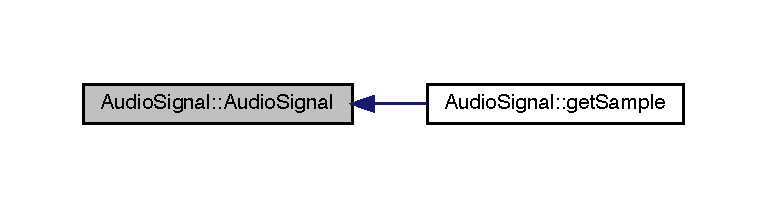
\includegraphics[width=350pt]{class_audio_signal_a72df7e0c092777d7b829ee7229d5d6f8_icgraph}
\end{center}
\end{figure}
\mbox{\Hypertarget{class_audio_signal_a755ad45352e2b260a2ee7fde2440a486}\label{class_audio_signal_a755ad45352e2b260a2ee7fde2440a486}} 
\index{Audio\+Signal@{Audio\+Signal}!Audio\+Signal@{Audio\+Signal}}
\index{Audio\+Signal@{Audio\+Signal}!Audio\+Signal@{Audio\+Signal}}
\subsubsection{\texorpdfstring{Audio\+Signal()}{AudioSignal()}\hspace{0.1cm}{\footnotesize\ttfamily [2/2]}}
{\footnotesize\ttfamily Audio\+Signal\+::\+Audio\+Signal (\begin{DoxyParamCaption}\item[{std\+::vector$<$ float $>$}]{signal,  }\item[{int}]{fs }\end{DoxyParamCaption})}


\begin{DoxyParams}{Parameters}
{\em signal} & vector of signal samples \\
\hline
{\em fs} & signal sampling frequency \mbox{[}Hz\mbox{]} \\
\hline
\end{DoxyParams}


Definition at line 29 of file Audio\+Signal.\+cpp.



\subsection{Member Function Documentation}
\mbox{\Hypertarget{class_audio_signal_a94c974f752e3045190944860bd8b0ad8}\label{class_audio_signal_a94c974f752e3045190944860bd8b0ad8}} 
\index{Audio\+Signal@{Audio\+Signal}!add\+Sample@{add\+Sample}}
\index{add\+Sample@{add\+Sample}!Audio\+Signal@{Audio\+Signal}}
\subsubsection{\texorpdfstring{add\+Sample()}{addSample()}}
{\footnotesize\ttfamily void Audio\+Signal\+::add\+Sample (\begin{DoxyParamCaption}\item[{float}]{sample }\end{DoxyParamCaption})}


\begin{DoxyParams}{Parameters}
{\em sample} & new signal sample \\
\hline
\end{DoxyParams}


Definition at line 89 of file Audio\+Signal.\+cpp.

Here is the call graph for this function\+:
\nopagebreak
\begin{figure}[H]
\begin{center}
\leavevmode
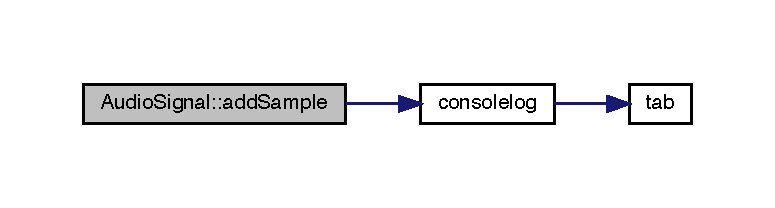
\includegraphics[width=350pt]{class_audio_signal_a94c974f752e3045190944860bd8b0ad8_cgraph}
\end{center}
\end{figure}
\mbox{\Hypertarget{class_audio_signal_aac1c34bc8bfcf31fdbac847e67cbea7f}\label{class_audio_signal_aac1c34bc8bfcf31fdbac847e67cbea7f}} 
\index{Audio\+Signal@{Audio\+Signal}!delete\+Sample@{delete\+Sample}}
\index{delete\+Sample@{delete\+Sample}!Audio\+Signal@{Audio\+Signal}}
\subsubsection{\texorpdfstring{delete\+Sample()}{deleteSample()}\hspace{0.1cm}{\footnotesize\ttfamily [1/2]}}
{\footnotesize\ttfamily void Audio\+Signal\+::delete\+Sample (\begin{DoxyParamCaption}\item[{int}]{index }\end{DoxyParamCaption})}


\begin{DoxyParams}{Parameters}
{\em index} & sample position index \\
\hline
\end{DoxyParams}


Definition at line 104 of file Audio\+Signal.\+cpp.

\mbox{\Hypertarget{class_audio_signal_a0c12f9dab81440c887138f8308d5f3b6}\label{class_audio_signal_a0c12f9dab81440c887138f8308d5f3b6}} 
\index{Audio\+Signal@{Audio\+Signal}!delete\+Sample@{delete\+Sample}}
\index{delete\+Sample@{delete\+Sample}!Audio\+Signal@{Audio\+Signal}}
\subsubsection{\texorpdfstring{delete\+Sample()}{deleteSample()}\hspace{0.1cm}{\footnotesize\ttfamily [2/2]}}
{\footnotesize\ttfamily void Audio\+Signal\+::delete\+Sample (\begin{DoxyParamCaption}\item[{int}]{start,  }\item[{int}]{end }\end{DoxyParamCaption})}


\begin{DoxyParams}{Parameters}
{\em start} & first index of the range (included) \\
\hline
{\em end} & last index of the range (included) \\
\hline
\end{DoxyParams}


Definition at line 114 of file Audio\+Signal.\+cpp.

\mbox{\Hypertarget{class_audio_signal_a4e45a4b1adc16a9cbd65501efafb6ded}\label{class_audio_signal_a4e45a4b1adc16a9cbd65501efafb6ded}} 
\index{Audio\+Signal@{Audio\+Signal}!get\+Frequencies@{get\+Frequencies}}
\index{get\+Frequencies@{get\+Frequencies}!Audio\+Signal@{Audio\+Signal}}
\subsubsection{\texorpdfstring{get\+Frequencies()}{getFrequencies()}\hspace{0.1cm}{\footnotesize\ttfamily [1/2]}}
{\footnotesize\ttfamily std\+::vector$<$ float $>$ Audio\+Signal\+::get\+Frequencies (\begin{DoxyParamCaption}{ }\end{DoxyParamCaption})}

\begin{DoxyReturn}{Returns}
frequencies vector 
\end{DoxyReturn}


Definition at line 227 of file Audio\+Signal.\+cpp.

Here is the caller graph for this function\+:
\nopagebreak
\begin{figure}[H]
\begin{center}
\leavevmode
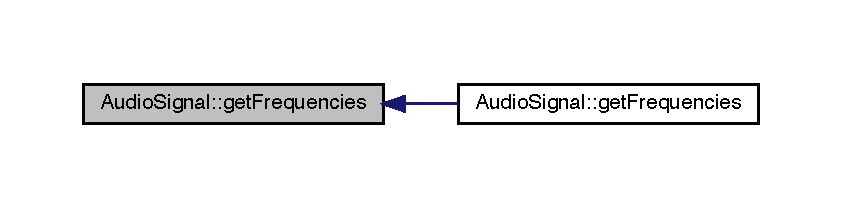
\includegraphics[width=350pt]{class_audio_signal_a4e45a4b1adc16a9cbd65501efafb6ded_icgraph}
\end{center}
\end{figure}
\mbox{\Hypertarget{class_audio_signal_a9b7d7a655913f579c0df8b2639b3ce56}\label{class_audio_signal_a9b7d7a655913f579c0df8b2639b3ce56}} 
\index{Audio\+Signal@{Audio\+Signal}!get\+Frequencies@{get\+Frequencies}}
\index{get\+Frequencies@{get\+Frequencies}!Audio\+Signal@{Audio\+Signal}}
\subsubsection{\texorpdfstring{get\+Frequencies()}{getFrequencies()}\hspace{0.1cm}{\footnotesize\ttfamily [2/2]}}
{\footnotesize\ttfamily std\+::vector$<$ float $>$ Audio\+Signal\+::get\+Frequencies (\begin{DoxyParamCaption}\item[{int}]{bands }\end{DoxyParamCaption})}


\begin{DoxyParams}{Parameters}
{\em bands} & number of frequency bands of the signal spectral density (if higher number than available has been requested, it returns as the highest number of frequency as possible) \\
\hline
\end{DoxyParams}
\begin{DoxyReturn}{Returns}
frequencies vector 
\end{DoxyReturn}


Definition at line 241 of file Audio\+Signal.\+cpp.

Here is the call graph for this function\+:
\nopagebreak
\begin{figure}[H]
\begin{center}
\leavevmode
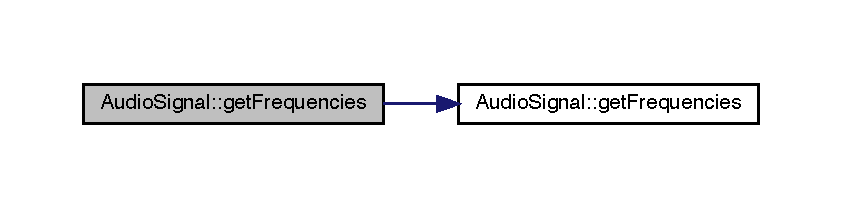
\includegraphics[width=350pt]{class_audio_signal_a9b7d7a655913f579c0df8b2639b3ce56_cgraph}
\end{center}
\end{figure}
\mbox{\Hypertarget{class_audio_signal_adfa4565e6ff0d8dc6bcbf87dbf6d01d1}\label{class_audio_signal_adfa4565e6ff0d8dc6bcbf87dbf6d01d1}} 
\index{Audio\+Signal@{Audio\+Signal}!get\+Sample@{get\+Sample}}
\index{get\+Sample@{get\+Sample}!Audio\+Signal@{Audio\+Signal}}
\subsubsection{\texorpdfstring{get\+Sample()}{getSample()}}
{\footnotesize\ttfamily \hyperlink{class_audio_signal}{Audio\+Signal} Audio\+Signal\+::get\+Sample (\begin{DoxyParamCaption}\item[{int}]{start,  }\item[{int}]{end }\end{DoxyParamCaption})}


\begin{DoxyParams}{Parameters}
{\em start} & first index of the range (included) \\
\hline
{\em end} & last index of the range (included) \\
\hline
\end{DoxyParams}
\begin{DoxyReturn}{Returns}
subsignal object 
\end{DoxyReturn}


Definition at line 64 of file Audio\+Signal.\+cpp.

Here is the call graph for this function\+:
\nopagebreak
\begin{figure}[H]
\begin{center}
\leavevmode
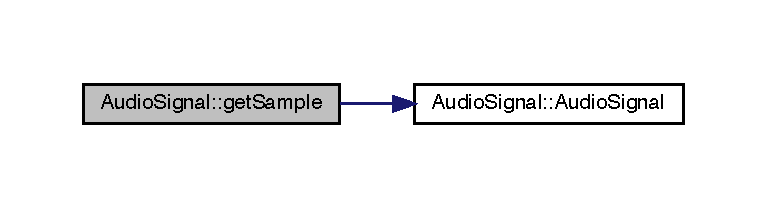
\includegraphics[width=350pt]{class_audio_signal_adfa4565e6ff0d8dc6bcbf87dbf6d01d1_cgraph}
\end{center}
\end{figure}
\mbox{\Hypertarget{class_audio_signal_aa86d766d3fe58e23a852751bbe2ecc78}\label{class_audio_signal_aa86d766d3fe58e23a852751bbe2ecc78}} 
\index{Audio\+Signal@{Audio\+Signal}!get\+Signal@{get\+Signal}}
\index{get\+Signal@{get\+Signal}!Audio\+Signal@{Audio\+Signal}}
\subsubsection{\texorpdfstring{get\+Signal()}{getSignal()}}
{\footnotesize\ttfamily std\+::vector$<$ float $>$ Audio\+Signal\+::get\+Signal (\begin{DoxyParamCaption}{ }\end{DoxyParamCaption})}

\begin{DoxyReturn}{Returns}
audio signal 
\end{DoxyReturn}


Definition at line 124 of file Audio\+Signal.\+cpp.

\mbox{\Hypertarget{class_audio_signal_a1c1330b11b635cfafe2edb75fd0d2e70}\label{class_audio_signal_a1c1330b11b635cfafe2edb75fd0d2e70}} 
\index{Audio\+Signal@{Audio\+Signal}!get\+Spectrum@{get\+Spectrum}}
\index{get\+Spectrum@{get\+Spectrum}!Audio\+Signal@{Audio\+Signal}}
\subsubsection{\texorpdfstring{get\+Spectrum()}{getSpectrum()}\hspace{0.1cm}{\footnotesize\ttfamily [1/2]}}
{\footnotesize\ttfamily std\+::vector$<$ float $>$ Audio\+Signal\+::get\+Spectrum (\begin{DoxyParamCaption}{ }\end{DoxyParamCaption})}

\begin{DoxyReturn}{Returns}
signal spectral density 
\end{DoxyReturn}


Definition at line 169 of file Audio\+Signal.\+cpp.

Here is the caller graph for this function\+:
\nopagebreak
\begin{figure}[H]
\begin{center}
\leavevmode
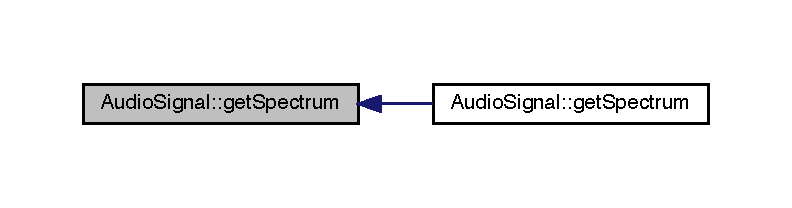
\includegraphics[width=350pt]{class_audio_signal_a1c1330b11b635cfafe2edb75fd0d2e70_icgraph}
\end{center}
\end{figure}
\mbox{\Hypertarget{class_audio_signal_ae49bd4dc391e6ae0e8a673ff8d5089fb}\label{class_audio_signal_ae49bd4dc391e6ae0e8a673ff8d5089fb}} 
\index{Audio\+Signal@{Audio\+Signal}!get\+Spectrum@{get\+Spectrum}}
\index{get\+Spectrum@{get\+Spectrum}!Audio\+Signal@{Audio\+Signal}}
\subsubsection{\texorpdfstring{get\+Spectrum()}{getSpectrum()}\hspace{0.1cm}{\footnotesize\ttfamily [2/2]}}
{\footnotesize\ttfamily std\+::vector$<$ float $>$ Audio\+Signal\+::get\+Spectrum (\begin{DoxyParamCaption}\item[{int}]{bands }\end{DoxyParamCaption})}


\begin{DoxyParams}{Parameters}
{\em bands} & number of frequency bands of the signal spectral density (if higher number than available has been requested, it returns as the highest number of frequency as possible) \\
\hline
\end{DoxyParams}
\begin{DoxyReturn}{Returns}
signal spectral density 
\end{DoxyReturn}


Definition at line 195 of file Audio\+Signal.\+cpp.

Here is the call graph for this function\+:
\nopagebreak
\begin{figure}[H]
\begin{center}
\leavevmode
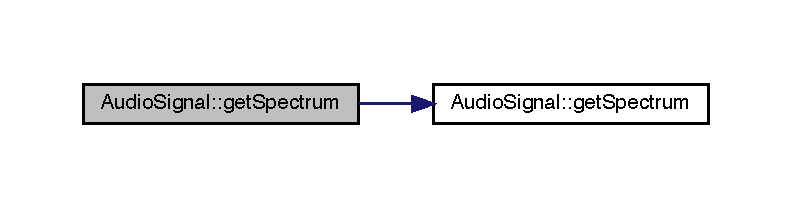
\includegraphics[width=350pt]{class_audio_signal_ae49bd4dc391e6ae0e8a673ff8d5089fb_cgraph}
\end{center}
\end{figure}
\mbox{\Hypertarget{class_audio_signal_afff46a70335800ba93ae513bdea7e4c9}\label{class_audio_signal_afff46a70335800ba93ae513bdea7e4c9}} 
\index{Audio\+Signal@{Audio\+Signal}!get\+Times@{get\+Times}}
\index{get\+Times@{get\+Times}!Audio\+Signal@{Audio\+Signal}}
\subsubsection{\texorpdfstring{get\+Times()}{getTimes()}\hspace{0.1cm}{\footnotesize\ttfamily [1/2]}}
{\footnotesize\ttfamily std\+::vector$<$ float $>$ Audio\+Signal\+::get\+Times (\begin{DoxyParamCaption}{ }\end{DoxyParamCaption})}

\begin{DoxyReturn}{Returns}
time vector 
\end{DoxyReturn}


Definition at line 141 of file Audio\+Signal.\+cpp.

\mbox{\Hypertarget{class_audio_signal_aa04d6fcd3219f4bb8d77916c60d85ad2}\label{class_audio_signal_aa04d6fcd3219f4bb8d77916c60d85ad2}} 
\index{Audio\+Signal@{Audio\+Signal}!get\+Times@{get\+Times}}
\index{get\+Times@{get\+Times}!Audio\+Signal@{Audio\+Signal}}
\subsubsection{\texorpdfstring{get\+Times()}{getTimes()}\hspace{0.1cm}{\footnotesize\ttfamily [2/2]}}
{\footnotesize\ttfamily std\+::vector$<$ float $>$ Audio\+Signal\+::get\+Times (\begin{DoxyParamCaption}\item[{float}]{initialtime }\end{DoxyParamCaption})}


\begin{DoxyParams}{Parameters}
{\em initialtime} & initial time \mbox{[}s\mbox{]} \\
\hline
\end{DoxyParams}
\begin{DoxyReturn}{Returns}
time vector 
\end{DoxyReturn}


Definition at line 155 of file Audio\+Signal.\+cpp.

\mbox{\Hypertarget{class_audio_signal_a92f6f979d43fe72d965e17b86dd82e79}\label{class_audio_signal_a92f6f979d43fe72d965e17b86dd82e79}} 
\index{Audio\+Signal@{Audio\+Signal}!operator\mbox{[}\mbox{]}@{operator[]}}
\index{operator\mbox{[}\mbox{]}@{operator[]}!Audio\+Signal@{Audio\+Signal}}
\subsubsection{\texorpdfstring{operator[]()}{operator[]()}}
{\footnotesize\ttfamily float Audio\+Signal\+::operator\mbox{[}$\,$\mbox{]} (\begin{DoxyParamCaption}\item[{int}]{index }\end{DoxyParamCaption})}


\begin{DoxyParams}{Parameters}
{\em index} & selected index \\
\hline
\end{DoxyParams}
\begin{DoxyReturn}{Returns}
sample signal sample 
\end{DoxyReturn}


Definition at line 46 of file Audio\+Signal.\+cpp.

Here is the call graph for this function\+:
\nopagebreak
\begin{figure}[H]
\begin{center}
\leavevmode
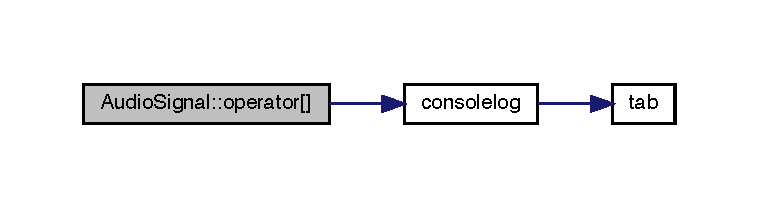
\includegraphics[width=350pt]{class_audio_signal_a92f6f979d43fe72d965e17b86dd82e79_cgraph}
\end{center}
\end{figure}
\mbox{\Hypertarget{class_audio_signal_aeef099025639235c7f062294470a691f}\label{class_audio_signal_aeef099025639235c7f062294470a691f}} 
\index{Audio\+Signal@{Audio\+Signal}!set\+Sample@{set\+Sample}}
\index{set\+Sample@{set\+Sample}!Audio\+Signal@{Audio\+Signal}}
\subsubsection{\texorpdfstring{set\+Sample()}{setSample()}}
{\footnotesize\ttfamily void Audio\+Signal\+::set\+Sample (\begin{DoxyParamCaption}\item[{int}]{index,  }\item[{float}]{sample }\end{DoxyParamCaption})}


\begin{DoxyParams}{Parameters}
{\em index} & selected index \\
\hline
{\em sample} & new signal sample \\
\hline
\end{DoxyParams}


Definition at line 76 of file Audio\+Signal.\+cpp.

Here is the call graph for this function\+:
\nopagebreak
\begin{figure}[H]
\begin{center}
\leavevmode
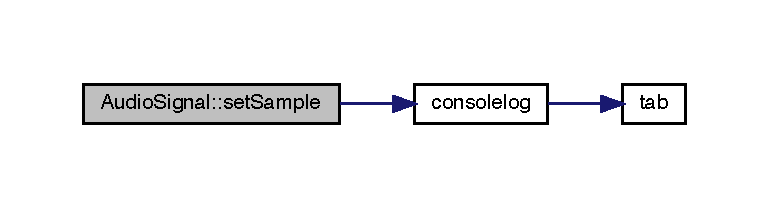
\includegraphics[width=350pt]{class_audio_signal_aeef099025639235c7f062294470a691f_cgraph}
\end{center}
\end{figure}
\mbox{\Hypertarget{class_audio_signal_a90eda59db04d3b18bd1949b8fa9e9c81}\label{class_audio_signal_a90eda59db04d3b18bd1949b8fa9e9c81}} 
\index{Audio\+Signal@{Audio\+Signal}!set\+Signal@{set\+Signal}}
\index{set\+Signal@{set\+Signal}!Audio\+Signal@{Audio\+Signal}}
\subsubsection{\texorpdfstring{set\+Signal()}{setSignal()}}
{\footnotesize\ttfamily void Audio\+Signal\+::set\+Signal (\begin{DoxyParamCaption}\item[{std\+::vector$<$ float $>$}]{signal }\end{DoxyParamCaption})}


\begin{DoxyParams}{Parameters}
{\em signal} & audio signal \\
\hline
\end{DoxyParams}


Definition at line 132 of file Audio\+Signal.\+cpp.



\subsection{Member Data Documentation}
\mbox{\Hypertarget{class_audio_signal_acc2dc31d0dc3ca222df68a88c00cf2c9}\label{class_audio_signal_acc2dc31d0dc3ca222df68a88c00cf2c9}} 
\index{Audio\+Signal@{Audio\+Signal}!fs@{fs}}
\index{fs@{fs}!Audio\+Signal@{Audio\+Signal}}
\subsubsection{\texorpdfstring{fs}{fs}}
{\footnotesize\ttfamily int Audio\+Signal\+::fs}

signal sampling frequency \mbox{[}Hz\mbox{]} 

Definition at line 20 of file Audio\+Signal.\+h.

\mbox{\Hypertarget{class_audio_signal_a5d68faf1ab7f19197b93cc2cc0a7e645}\label{class_audio_signal_a5d68faf1ab7f19197b93cc2cc0a7e645}} 
\index{Audio\+Signal@{Audio\+Signal}!maxsamples@{maxsamples}}
\index{maxsamples@{maxsamples}!Audio\+Signal@{Audio\+Signal}}
\subsubsection{\texorpdfstring{maxsamples}{maxsamples}}
{\footnotesize\ttfamily const unsigned int Audio\+Signal\+::maxsamples = 0x\+F\+F\+F\+F\+FF\hspace{0.3cm}{\ttfamily [static]}}

maximum number of samples 

Definition at line 21 of file Audio\+Signal.\+h.

\mbox{\Hypertarget{class_audio_signal_a44e595328705720f380613f1675dbdd1}\label{class_audio_signal_a44e595328705720f380613f1675dbdd1}} 
\index{Audio\+Signal@{Audio\+Signal}!size@{size}}
\index{size@{size}!Audio\+Signal@{Audio\+Signal}}
\subsubsection{\texorpdfstring{size}{size}}
{\footnotesize\ttfamily int Audio\+Signal\+::size}

number of samples 

Definition at line 19 of file Audio\+Signal.\+h.



The documentation for this class was generated from the following files\+:\begin{DoxyCompactItemize}
\item 
src/process/Audio\+Signal.\+h\item 
src/process/Audio\+Signal.\+cpp\end{DoxyCompactItemize}

\hypertarget{class_audio_test}{}\section{Audio\+Test Class Reference}
\label{class_audio_test}\index{Audio\+Test@{Audio\+Test}}


Audio output test class.  




{\ttfamily \#include $<$Audio\+Output.\+h$>$}



Inheritance diagram for Audio\+Test\+:
\nopagebreak
\begin{figure}[H]
\begin{center}
\leavevmode
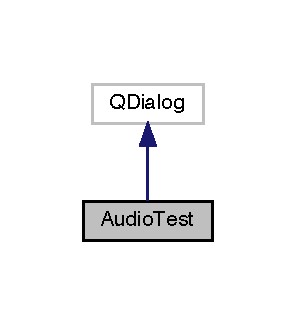
\includegraphics[width=142pt]{class_audio_test__inherit__graph}
\end{center}
\end{figure}


Collaboration diagram for Audio\+Test\+:
\nopagebreak
\begin{figure}[H]
\begin{center}
\leavevmode
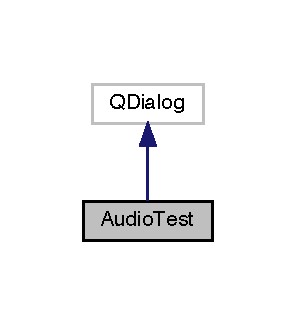
\includegraphics[width=142pt]{class_audio_test__coll__graph}
\end{center}
\end{figure}
\subsection*{Public Member Functions}
\begin{DoxyCompactItemize}
\item 
\hyperlink{class_audio_test_a8732c48308ca1352a4d89803553b395e}{Audio\+Test} (Q\+Widget $\ast$parent=0)
\begin{DoxyCompactList}\small\item\em \hyperlink{class_audio_test}{Audio\+Test} constructor. \end{DoxyCompactList}\item 
\mbox{\Hypertarget{class_audio_test_ae37879db71b1540d84aa37a093978192}\label{class_audio_test_ae37879db71b1540d84aa37a093978192}} 
\hyperlink{class_audio_test_ae37879db71b1540d84aa37a093978192}{$\sim$\+Audio\+Test} ()
\begin{DoxyCompactList}\small\item\em \hyperlink{class_audio_test}{Audio\+Test} destructor. \end{DoxyCompactList}\end{DoxyCompactItemize}


\subsection{Detailed Description}
\begin{DoxyAuthor}{Author}
Andrés González Fornell 
\end{DoxyAuthor}


Definition at line 88 of file Audio\+Output.\+h.



\subsection{Constructor \& Destructor Documentation}
\mbox{\Hypertarget{class_audio_test_a8732c48308ca1352a4d89803553b395e}\label{class_audio_test_a8732c48308ca1352a4d89803553b395e}} 
\index{Audio\+Test@{Audio\+Test}!Audio\+Test@{Audio\+Test}}
\index{Audio\+Test@{Audio\+Test}!Audio\+Test@{Audio\+Test}}
\subsubsection{\texorpdfstring{Audio\+Test()}{AudioTest()}}
{\footnotesize\ttfamily Audio\+Test\+::\+Audio\+Test (\begin{DoxyParamCaption}\item[{Q\+Widget $\ast$}]{parent = {\ttfamily 0} }\end{DoxyParamCaption})}


\begin{DoxyParams}{Parameters}
{\em parent} & window parent \\
\hline
\end{DoxyParams}


Definition at line 298 of file Audio\+Output.\+cpp.

Here is the call graph for this function\+:
\nopagebreak
\begin{figure}[H]
\begin{center}
\leavevmode
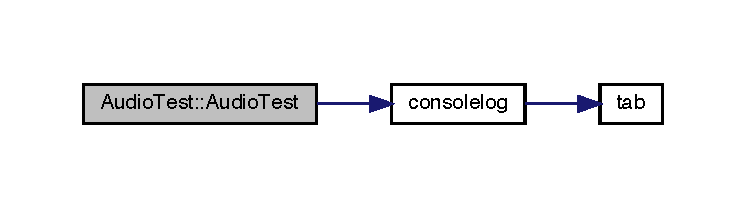
\includegraphics[width=350pt]{class_audio_test_a8732c48308ca1352a4d89803553b395e_cgraph}
\end{center}
\end{figure}


The documentation for this class was generated from the following files\+:\begin{DoxyCompactItemize}
\item 
src/interface/Audio\+Output.\+h\item 
src/interface/Audio\+Output.\+cpp\end{DoxyCompactItemize}

\hypertarget{struct_binaural_quality}{}\section{Binaural\+Quality Struct Reference}
\label{struct_binaural_quality}\index{Binaural\+Quality@{Binaural\+Quality}}


S\+AC decoder parameter binaural quality.  




{\ttfamily \#include $<$S\+A\+C\+Effects.\+h$>$}

\subsection*{Public Types}
\begin{DoxyCompactItemize}
\item 
enum \hyperlink{struct_binaural_quality_a3a009a287684c778dbb5507226cf24e4}{binauralquality} \{ {\bfseries parametric} = 0, 
\hyperlink{struct_binaural_quality_a3a009a287684c778dbb5507226cf24e4a4f6f52196ab75b6d1b20df0d796807fc}{filtering} = 1
 \}
\end{DoxyCompactItemize}


\subsection{Detailed Description}


Definition at line 46 of file S\+A\+C\+Effects.\+h.



\subsection{Member Enumeration Documentation}
\mbox{\Hypertarget{struct_binaural_quality_a3a009a287684c778dbb5507226cf24e4}\label{struct_binaural_quality_a3a009a287684c778dbb5507226cf24e4}} 
\index{Binaural\+Quality@{Binaural\+Quality}!binauralquality@{binauralquality}}
\index{binauralquality@{binauralquality}!Binaural\+Quality@{Binaural\+Quality}}
\subsubsection{\texorpdfstring{binauralquality}{binauralquality}}
{\footnotesize\ttfamily enum \hyperlink{struct_binaural_quality_a3a009a287684c778dbb5507226cf24e4}{Binaural\+Quality\+::binauralquality}}

\begin{DoxyEnumFields}{Enumerator}
\raisebox{\heightof{T}}[0pt][0pt]{\index{filtering@{filtering}!Binaural\+Quality@{Binaural\+Quality}}\index{Binaural\+Quality@{Binaural\+Quality}!filtering@{filtering}}}\mbox{\Hypertarget{struct_binaural_quality_a3a009a287684c778dbb5507226cf24e4a4f6f52196ab75b6d1b20df0d796807fc}\label{struct_binaural_quality_a3a009a287684c778dbb5507226cf24e4a4f6f52196ab75b6d1b20df0d796807fc}} 
filtering&parametric binaural quality filtering binaural quality \\
\hline

\end{DoxyEnumFields}


Definition at line 47 of file S\+A\+C\+Effects.\+h.



The documentation for this struct was generated from the following file\+:\begin{DoxyCompactItemize}
\item 
src/interface/S\+A\+C\+Effects.\+h\end{DoxyCompactItemize}

\hypertarget{class_channel}{}\section{Channel Class Reference}
\label{class_channel}\index{Channel@{Channel}}


Single-\/object class from channels list.  




{\ttfamily \#include $<$Channels\+List.\+h$>$}



Collaboration diagram for Channel\+:
\nopagebreak
\begin{figure}[H]
\begin{center}
\leavevmode
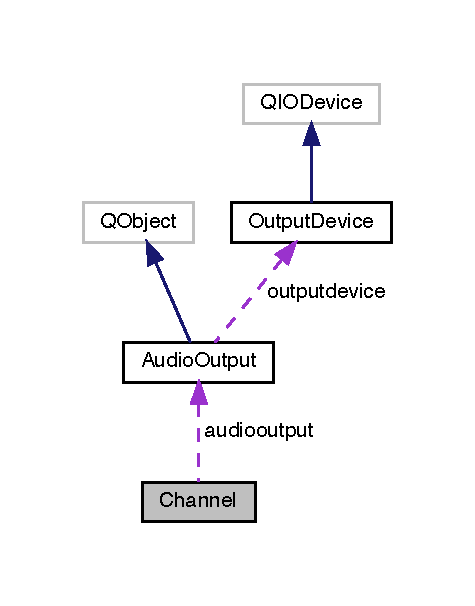
\includegraphics[width=228pt]{class_channel__coll__graph}
\end{center}
\end{figure}
\subsection*{Public Member Functions}
\begin{DoxyCompactItemize}
\item 
\hyperlink{class_channel_a3a5079024e870e5188f7af98772ae38c}{Channel} (Q\+Layout $\ast$framework, std\+::string prefix, int \hyperlink{class_channel_a992b8f195f395a64b4e966886bb41f00}{index}, bool isoutput)
\begin{DoxyCompactList}\small\item\em Channels constructor. \end{DoxyCompactList}\item 
\mbox{\Hypertarget{class_channel_a5f15ebd302464069f1a9e3f0ded14482}\label{class_channel_a5f15ebd302464069f1a9e3f0ded14482}} 
\hyperlink{class_channel_a5f15ebd302464069f1a9e3f0ded14482}{$\sim$\+Channel} ()
\begin{DoxyCompactList}\small\item\em Channels desctructor. \end{DoxyCompactList}\item 
int \hyperlink{class_channel_af0427a10e1713ba8327df0b0cd0fb2f5}{get\+Index} ()
\begin{DoxyCompactList}\small\item\em It gets the channel index. \end{DoxyCompactList}\item 
\mbox{\Hypertarget{class_channel_a21286e2c4add83ea96e2636e87e9871b}\label{class_channel_a21286e2c4add83ea96e2636e87e9871b}} 
void {\bfseries set\+Index} (int \hyperlink{class_channel_a992b8f195f395a64b4e966886bb41f00}{index})
\item 
void \hyperlink{class_channel_a1d0ac75e7416c18c3695de418e9137e1}{set\+Label} (std\+::string \hyperlink{class_channel_a66a7e30d0b8c6ee9c0b0d537b59bd695}{label})
\begin{DoxyCompactList}\small\item\em It sets a label to the channel name, i.\+e., group box title and label text. \end{DoxyCompactList}\item 
void \hyperlink{class_channel_a381d4ad81038cb9bcf393fa47b13cdb0}{set\+Volume} (int \hyperlink{class_channel_aa8977e4605932b2201b03ebf3aa14ffd}{volume})
\begin{DoxyCompactList}\small\item\em It sets the channel volume level. \end{DoxyCompactList}\item 
void \hyperlink{class_channel_a88f542e0f6d1e1d384ad8bf79a9e305b}{mute} (bool state)
\begin{DoxyCompactList}\small\item\em It mutes channel. \end{DoxyCompactList}\item 
void \hyperlink{class_channel_a2574d67b3f0d3f90c04a6154b96e303a}{bypass} (bool state)
\begin{DoxyCompactList}\small\item\em It sets channel to bypass effects. \end{DoxyCompactList}\end{DoxyCompactItemize}
\subsection*{Public Attributes}
\begin{DoxyCompactItemize}
\item 
int \hyperlink{class_channel_a992b8f195f395a64b4e966886bb41f00}{index}
\item 
std\+::string \hyperlink{class_channel_ae080e1afd52f3b70e04c62fea46447aa}{name}
\item 
double \hyperlink{class_channel_aa8977e4605932b2201b03ebf3aa14ffd}{volume}
\item 
bool \hyperlink{class_channel_ada7e3a050c346ad283ad302745f03f3c}{muted}
\item 
bool \hyperlink{class_channel_a94507945240717f2570e3baadd02d08a}{bypassed}
\item 
\hyperlink{class_audio_output}{Audio\+Output} $\ast$ \hyperlink{class_channel_a7c8a0b25848ab487c39a803785f7ed21}{audiooutput}
\end{DoxyCompactItemize}
\textbf{ }\par
\begin{DoxyCompactItemize}
\item 
Q\+Group\+Box $\ast$ \hyperlink{class_channel_a99287738754d9e20c0ca639d6d26f28c}{groupbox}
\begin{DoxyCompactList}\small\item\em user interface elements \end{DoxyCompactList}\item 
Q\+Line\+Edit $\ast$ \hyperlink{class_channel_a66a7e30d0b8c6ee9c0b0d537b59bd695}{label}
\item 
Q\+Slider $\ast$ \hyperlink{class_channel_acbcbfb33558a69224daa176372eb8be3}{volumeslider}
\item 
Q\+Check\+Box $\ast$ \hyperlink{class_channel_a0e7f90da49f291a7bac498e11e886fbd}{mutecheckbox}
\item 
Q\+Check\+Box $\ast$ \hyperlink{class_channel_a285eab1752d5e9407e1bc1e75353df34}{bypasscheckbox}
\item 
Q\+Combo\+Box $\ast$ \hyperlink{class_channel_a9dcb50dc41866fbe60424553f1b910fa}{deviceselector}
\end{DoxyCompactItemize}



\subsection{Detailed Description}
\begin{DoxyAuthor}{Author}
Andrés González Fornell 
\end{DoxyAuthor}


Definition at line 32 of file Channels\+List.\+h.



\subsection{Constructor \& Destructor Documentation}
\mbox{\Hypertarget{class_channel_a3a5079024e870e5188f7af98772ae38c}\label{class_channel_a3a5079024e870e5188f7af98772ae38c}} 
\index{Channel@{Channel}!Channel@{Channel}}
\index{Channel@{Channel}!Channel@{Channel}}
\subsubsection{\texorpdfstring{Channel()}{Channel()}}
{\footnotesize\ttfamily Channel\+::\+Channel (\begin{DoxyParamCaption}\item[{Q\+Layout $\ast$}]{framework,  }\item[{std\+::string}]{prefix,  }\item[{int}]{index,  }\item[{bool}]{isoutput }\end{DoxyParamCaption})}


\begin{DoxyParams}{Parameters}
{\em framework} & channel user interface framework \\
\hline
{\em prefix} & prefix of objects name of channel user interface \\
\hline
{\em index} & channel index \\
\hline
{\em isoutput} & true to create device selector to send audio to the system audio output devices \\
\hline
\end{DoxyParams}


Definition at line 213 of file Channels\+List.\+cpp.

Here is the call graph for this function\+:
\nopagebreak
\begin{figure}[H]
\begin{center}
\leavevmode
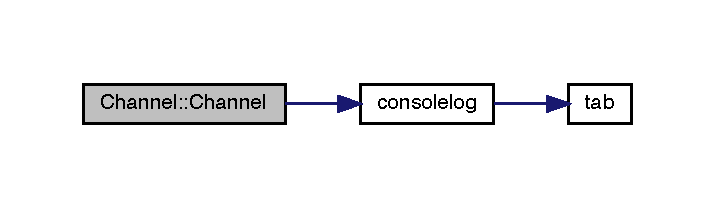
\includegraphics[width=343pt]{class_channel_a3a5079024e870e5188f7af98772ae38c_cgraph}
\end{center}
\end{figure}


\subsection{Member Function Documentation}
\mbox{\Hypertarget{class_channel_a2574d67b3f0d3f90c04a6154b96e303a}\label{class_channel_a2574d67b3f0d3f90c04a6154b96e303a}} 
\index{Channel@{Channel}!bypass@{bypass}}
\index{bypass@{bypass}!Channel@{Channel}}
\subsubsection{\texorpdfstring{bypass()}{bypass()}}
{\footnotesize\ttfamily void Channel\+::bypass (\begin{DoxyParamCaption}\item[{bool}]{state }\end{DoxyParamCaption})}


\begin{DoxyParams}{Parameters}
{\em state} & true to bypass effects and false to apply them \\
\hline
\end{DoxyParams}


Definition at line 318 of file Channels\+List.\+cpp.

\mbox{\Hypertarget{class_channel_af0427a10e1713ba8327df0b0cd0fb2f5}\label{class_channel_af0427a10e1713ba8327df0b0cd0fb2f5}} 
\index{Channel@{Channel}!get\+Index@{get\+Index}}
\index{get\+Index@{get\+Index}!Channel@{Channel}}
\subsubsection{\texorpdfstring{get\+Index()}{getIndex()}}
{\footnotesize\ttfamily int Channel\+::get\+Index (\begin{DoxyParamCaption}{ }\end{DoxyParamCaption})}

\begin{DoxyReturn}{Returns}
index 
\end{DoxyReturn}


Definition at line 271 of file Channels\+List.\+cpp.

\mbox{\Hypertarget{class_channel_a88f542e0f6d1e1d384ad8bf79a9e305b}\label{class_channel_a88f542e0f6d1e1d384ad8bf79a9e305b}} 
\index{Channel@{Channel}!mute@{mute}}
\index{mute@{mute}!Channel@{Channel}}
\subsubsection{\texorpdfstring{mute()}{mute()}}
{\footnotesize\ttfamily void Channel\+::mute (\begin{DoxyParamCaption}\item[{bool}]{state }\end{DoxyParamCaption})}


\begin{DoxyParams}{Parameters}
{\em state} & true to mute the channel and false to unmuted \\
\hline
\end{DoxyParams}


Definition at line 309 of file Channels\+List.\+cpp.

\mbox{\Hypertarget{class_channel_a1d0ac75e7416c18c3695de418e9137e1}\label{class_channel_a1d0ac75e7416c18c3695de418e9137e1}} 
\index{Channel@{Channel}!set\+Label@{set\+Label}}
\index{set\+Label@{set\+Label}!Channel@{Channel}}
\subsubsection{\texorpdfstring{set\+Label()}{setLabel()}}
{\footnotesize\ttfamily void Channel\+::set\+Label (\begin{DoxyParamCaption}\item[{std\+::string}]{label }\end{DoxyParamCaption})}


\begin{DoxyParams}{Parameters}
{\em label} & new label \\
\hline
\end{DoxyParams}


Definition at line 297 of file Channels\+List.\+cpp.

\mbox{\Hypertarget{class_channel_a381d4ad81038cb9bcf393fa47b13cdb0}\label{class_channel_a381d4ad81038cb9bcf393fa47b13cdb0}} 
\index{Channel@{Channel}!set\+Volume@{set\+Volume}}
\index{set\+Volume@{set\+Volume}!Channel@{Channel}}
\subsubsection{\texorpdfstring{set\+Volume()}{setVolume()}}
{\footnotesize\ttfamily void Channel\+::set\+Volume (\begin{DoxyParamCaption}\item[{int}]{volume }\end{DoxyParamCaption})}


\begin{DoxyParams}{Parameters}
{\em volume} & integer number from 0 to 100 \\
\hline
\end{DoxyParams}


Definition at line 327 of file Channels\+List.\+cpp.



\subsection{Member Data Documentation}
\mbox{\Hypertarget{class_channel_a7c8a0b25848ab487c39a803785f7ed21}\label{class_channel_a7c8a0b25848ab487c39a803785f7ed21}} 
\index{Channel@{Channel}!audiooutput@{audiooutput}}
\index{audiooutput@{audiooutput}!Channel@{Channel}}
\subsubsection{\texorpdfstring{audiooutput}{audiooutput}}
{\footnotesize\ttfamily \hyperlink{class_audio_output}{Audio\+Output}$\ast$ Channel\+::audiooutput}

system audio output devices object 

Definition at line 39 of file Channels\+List.\+h.

\mbox{\Hypertarget{class_channel_a285eab1752d5e9407e1bc1e75353df34}\label{class_channel_a285eab1752d5e9407e1bc1e75353df34}} 
\index{Channel@{Channel}!bypasscheckbox@{bypasscheckbox}}
\index{bypasscheckbox@{bypasscheckbox}!Channel@{Channel}}
\subsubsection{\texorpdfstring{bypasscheckbox}{bypasscheckbox}}
{\footnotesize\ttfamily Q\+Check\+Box$\ast$ Channel\+::bypasscheckbox}

checkbox object to bypass effect 

Definition at line 48 of file Channels\+List.\+h.

\mbox{\Hypertarget{class_channel_a94507945240717f2570e3baadd02d08a}\label{class_channel_a94507945240717f2570e3baadd02d08a}} 
\index{Channel@{Channel}!bypassed@{bypassed}}
\index{bypassed@{bypassed}!Channel@{Channel}}
\subsubsection{\texorpdfstring{bypassed}{bypassed}}
{\footnotesize\ttfamily bool Channel\+::bypassed}

it tells channel to bypass effects or apply them 

Definition at line 38 of file Channels\+List.\+h.

\mbox{\Hypertarget{class_channel_a9dcb50dc41866fbe60424553f1b910fa}\label{class_channel_a9dcb50dc41866fbe60424553f1b910fa}} 
\index{Channel@{Channel}!deviceselector@{deviceselector}}
\index{deviceselector@{deviceselector}!Channel@{Channel}}
\subsubsection{\texorpdfstring{deviceselector}{deviceselector}}
{\footnotesize\ttfamily Q\+Combo\+Box$\ast$ Channel\+::deviceselector}

audio output device selector object 

Definition at line 49 of file Channels\+List.\+h.

\mbox{\Hypertarget{class_channel_a99287738754d9e20c0ca639d6d26f28c}\label{class_channel_a99287738754d9e20c0ca639d6d26f28c}} 
\index{Channel@{Channel}!groupbox@{groupbox}}
\index{groupbox@{groupbox}!Channel@{Channel}}
\subsubsection{\texorpdfstring{groupbox}{groupbox}}
{\footnotesize\ttfamily Q\+Group\+Box$\ast$ Channel\+::groupbox}

channel group box 

Definition at line 44 of file Channels\+List.\+h.

\mbox{\Hypertarget{class_channel_a992b8f195f395a64b4e966886bb41f00}\label{class_channel_a992b8f195f395a64b4e966886bb41f00}} 
\index{Channel@{Channel}!index@{index}}
\index{index@{index}!Channel@{Channel}}
\subsubsection{\texorpdfstring{index}{index}}
{\footnotesize\ttfamily int Channel\+::index}

channel index 

Definition at line 34 of file Channels\+List.\+h.

\mbox{\Hypertarget{class_channel_a66a7e30d0b8c6ee9c0b0d537b59bd695}\label{class_channel_a66a7e30d0b8c6ee9c0b0d537b59bd695}} 
\index{Channel@{Channel}!label@{label}}
\index{label@{label}!Channel@{Channel}}
\subsubsection{\texorpdfstring{label}{label}}
{\footnotesize\ttfamily Q\+Line\+Edit$\ast$ Channel\+::label}

field to change the channel label 

Definition at line 45 of file Channels\+List.\+h.

\mbox{\Hypertarget{class_channel_a0e7f90da49f291a7bac498e11e886fbd}\label{class_channel_a0e7f90da49f291a7bac498e11e886fbd}} 
\index{Channel@{Channel}!mutecheckbox@{mutecheckbox}}
\index{mutecheckbox@{mutecheckbox}!Channel@{Channel}}
\subsubsection{\texorpdfstring{mutecheckbox}{mutecheckbox}}
{\footnotesize\ttfamily Q\+Check\+Box$\ast$ Channel\+::mutecheckbox}

muted checkbox object 

Definition at line 47 of file Channels\+List.\+h.

\mbox{\Hypertarget{class_channel_ada7e3a050c346ad283ad302745f03f3c}\label{class_channel_ada7e3a050c346ad283ad302745f03f3c}} 
\index{Channel@{Channel}!muted@{muted}}
\index{muted@{muted}!Channel@{Channel}}
\subsubsection{\texorpdfstring{muted}{muted}}
{\footnotesize\ttfamily bool Channel\+::muted}

it indicates if channel is muted 

Definition at line 37 of file Channels\+List.\+h.

\mbox{\Hypertarget{class_channel_ae080e1afd52f3b70e04c62fea46447aa}\label{class_channel_ae080e1afd52f3b70e04c62fea46447aa}} 
\index{Channel@{Channel}!name@{name}}
\index{name@{name}!Channel@{Channel}}
\subsubsection{\texorpdfstring{name}{name}}
{\footnotesize\ttfamily std\+::string Channel\+::name}

channel name 

Definition at line 35 of file Channels\+List.\+h.

\mbox{\Hypertarget{class_channel_aa8977e4605932b2201b03ebf3aa14ffd}\label{class_channel_aa8977e4605932b2201b03ebf3aa14ffd}} 
\index{Channel@{Channel}!volume@{volume}}
\index{volume@{volume}!Channel@{Channel}}
\subsubsection{\texorpdfstring{volume}{volume}}
{\footnotesize\ttfamily double Channel\+::volume}

current audio volume level 

Definition at line 36 of file Channels\+List.\+h.

\mbox{\Hypertarget{class_channel_acbcbfb33558a69224daa176372eb8be3}\label{class_channel_acbcbfb33558a69224daa176372eb8be3}} 
\index{Channel@{Channel}!volumeslider@{volumeslider}}
\index{volumeslider@{volumeslider}!Channel@{Channel}}
\subsubsection{\texorpdfstring{volumeslider}{volumeslider}}
{\footnotesize\ttfamily Q\+Slider$\ast$ Channel\+::volumeslider}

volume level slider 

Definition at line 46 of file Channels\+List.\+h.



The documentation for this class was generated from the following files\+:\begin{DoxyCompactItemize}
\item 
src/interface/Channels\+List.\+h\item 
src/interface/Channels\+List.\+cpp\end{DoxyCompactItemize}

\section{Channels\+Charts Class Reference}
\label{class_channels_charts}\index{Channels\+Charts@{Channels\+Charts}}


{\ttfamily \#include $<$Channels\+List.\+h$>$}

Inheritance diagram for Channels\+Charts\+:\begin{figure}[H]
\begin{center}
\leavevmode
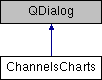
\includegraphics[height=2.000000cm]{class_channels_charts}
\end{center}
\end{figure}
\subsection*{Public Member Functions}
\begin{DoxyCompactItemize}
\item 
\textbf{ Channels\+Charts} (float $\ast$$\ast$\textbf{ input}, float $\ast$$\ast$\textbf{ output}, \textbf{ Channels\+List} $\ast$\textbf{ input\+\_\+channels}, \textbf{ Channels\+List} $\ast$\textbf{ output\+\_\+channels}, int \textbf{ samples}, Q\+Widget $\ast$parent=0)
\begin{DoxyCompactList}\small\item\em \doxyref{Channels\+Charts}{p.}{class_channels_charts} constructor. \end{DoxyCompactList}\item 
\textbf{ $\sim$\+Channels\+Charts} ()
\begin{DoxyCompactList}\small\item\em \doxyref{Channels\+Charts}{p.}{class_channels_charts} destructor. \end{DoxyCompactList}\end{DoxyCompactItemize}
\subsection*{Private Slots}
\begin{DoxyCompactItemize}
\item 
void \textbf{ set\+Time\+Cursor} (int sample)
\begin{DoxyCompactList}\small\item\em It sets the start time cursor. \end{DoxyCompactList}\item 
int \textbf{ get\+Time\+Cursor} ()
\begin{DoxyCompactList}\small\item\em It gets the start time cursor. \end{DoxyCompactList}\item 
void \textbf{ set\+Scope} (int time)
\begin{DoxyCompactList}\small\item\em It sets the charts scope. \end{DoxyCompactList}\item 
int \textbf{ get\+Scope} ()
\begin{DoxyCompactList}\small\item\em It gets the charts scope. \end{DoxyCompactList}\item 
void \textbf{ plot} ()
\begin{DoxyCompactList}\small\item\em It plots the current input and ouput signals. \end{DoxyCompactList}\end{DoxyCompactItemize}
\subsection*{Private Member Functions}
\begin{DoxyCompactItemize}
\item 
void \textbf{ update\+Selectors} ()
\begin{DoxyCompactList}\small\item\em It loads current channels names on chart selectors. \end{DoxyCompactList}\end{DoxyCompactItemize}
\subsection*{Private Attributes}
\begin{DoxyCompactItemize}
\item 
Ui\+::\+Channels\+Charts $\ast$ \textbf{ ui}
\item 
float $\ast$$\ast$ \textbf{ input}
\item 
float $\ast$$\ast$ \textbf{ output}
\item 
\textbf{ Channels\+List} $\ast$ \textbf{ input\+\_\+channels}
\item 
\textbf{ Channels\+List} $\ast$ \textbf{ output\+\_\+channels}
\item 
int \textbf{ samples}
\item 
\textbf{ Chart2D} $\ast$ \textbf{ input\+\_\+chart}
\item 
\textbf{ Chart2D} $\ast$ \textbf{ output\+\_\+chart}
\end{DoxyCompactItemize}


\subsection{Constructor \& Destructor Documentation}
\mbox{\label{class_channels_charts_a6fd985f15981dde4bca95c029ec3549f}} 
\index{Channels\+Charts@{Channels\+Charts}!Channels\+Charts@{Channels\+Charts}}
\index{Channels\+Charts@{Channels\+Charts}!Channels\+Charts@{Channels\+Charts}}
\subsubsection{Channels\+Charts()}
{\footnotesize\ttfamily Channels\+Charts\+::\+Channels\+Charts (\begin{DoxyParamCaption}\item[{float $\ast$$\ast$}]{input,  }\item[{float $\ast$$\ast$}]{output,  }\item[{\textbf{ Channels\+List} $\ast$}]{input\+\_\+channels,  }\item[{\textbf{ Channels\+List} $\ast$}]{output\+\_\+channels,  }\item[{int}]{samples,  }\item[{Q\+Widget $\ast$}]{parent = {\ttfamily 0} }\end{DoxyParamCaption})}



\doxyref{Channels\+Charts}{p.}{class_channels_charts} constructor. 


\begin{DoxyParams}{Parameters}
{\em input} & input signal pointer \\
\hline
{\em output} & output signal pointer \\
\hline
{\em input\+\_\+channels} & input channels object \\
\hline
{\em output\+\_\+channels} & output channels object \\
\hline
{\em samples} & number of samples each channel \\
\hline
{\em parent} & user inteface parent object \\
\hline
\end{DoxyParams}
\mbox{\label{class_channels_charts_a459f485f41a6734fe486358502cb8cca}} 
\index{Channels\+Charts@{Channels\+Charts}!````~Channels\+Charts@{$\sim$\+Channels\+Charts}}
\index{````~Channels\+Charts@{$\sim$\+Channels\+Charts}!Channels\+Charts@{Channels\+Charts}}
\subsubsection{$\sim$\+Channels\+Charts()}
{\footnotesize\ttfamily Channels\+Charts\+::$\sim$\+Channels\+Charts (\begin{DoxyParamCaption}{ }\end{DoxyParamCaption})}



\doxyref{Channels\+Charts}{p.}{class_channels_charts} destructor. 



\subsection{Member Function Documentation}
\mbox{\label{class_channels_charts_a7ff13f41cb1f81cb6458528c86cf7dee}} 
\index{Channels\+Charts@{Channels\+Charts}!get\+Scope@{get\+Scope}}
\index{get\+Scope@{get\+Scope}!Channels\+Charts@{Channels\+Charts}}
\subsubsection{get\+Scope}
{\footnotesize\ttfamily int Channels\+Charts\+::get\+Scope (\begin{DoxyParamCaption}{ }\end{DoxyParamCaption})\hspace{0.3cm}{\ttfamily [private]}, {\ttfamily [slot]}}



It gets the charts scope. 

\begin{DoxyReturn}{Returns}
number of sample of charts scope 
\end{DoxyReturn}
\mbox{\label{class_channels_charts_a576536e9799ff80e4680674bd0ac0d32}} 
\index{Channels\+Charts@{Channels\+Charts}!get\+Time\+Cursor@{get\+Time\+Cursor}}
\index{get\+Time\+Cursor@{get\+Time\+Cursor}!Channels\+Charts@{Channels\+Charts}}
\subsubsection{get\+Time\+Cursor}
{\footnotesize\ttfamily int Channels\+Charts\+::get\+Time\+Cursor (\begin{DoxyParamCaption}{ }\end{DoxyParamCaption})\hspace{0.3cm}{\ttfamily [private]}, {\ttfamily [slot]}}



It gets the start time cursor. 

\begin{DoxyReturn}{Returns}
first sample of the chart 
\end{DoxyReturn}
\mbox{\label{class_channels_charts_ab89ee4019f801400f7f965340f4970e5}} 
\index{Channels\+Charts@{Channels\+Charts}!plot@{plot}}
\index{plot@{plot}!Channels\+Charts@{Channels\+Charts}}
\subsubsection{plot}
{\footnotesize\ttfamily void Channels\+Charts\+::plot (\begin{DoxyParamCaption}{ }\end{DoxyParamCaption})\hspace{0.3cm}{\ttfamily [private]}, {\ttfamily [slot]}}



It plots the current input and ouput signals. 

\mbox{\label{class_channels_charts_a15f23882901d1a57dc6bc3d24a2f6924}} 
\index{Channels\+Charts@{Channels\+Charts}!set\+Scope@{set\+Scope}}
\index{set\+Scope@{set\+Scope}!Channels\+Charts@{Channels\+Charts}}
\subsubsection{set\+Scope}
{\footnotesize\ttfamily void Channels\+Charts\+::set\+Scope (\begin{DoxyParamCaption}\item[{int}]{time }\end{DoxyParamCaption})\hspace{0.3cm}{\ttfamily [private]}, {\ttfamily [slot]}}



It sets the charts scope. 


\begin{DoxyParams}{Parameters}
{\em time} & charts scope [ms] \\
\hline
\end{DoxyParams}
\mbox{\label{class_channels_charts_a2fbd3271e2cef600c24bf0f426a12ef0}} 
\index{Channels\+Charts@{Channels\+Charts}!set\+Time\+Cursor@{set\+Time\+Cursor}}
\index{set\+Time\+Cursor@{set\+Time\+Cursor}!Channels\+Charts@{Channels\+Charts}}
\subsubsection{set\+Time\+Cursor}
{\footnotesize\ttfamily void Channels\+Charts\+::set\+Time\+Cursor (\begin{DoxyParamCaption}\item[{int}]{sample }\end{DoxyParamCaption})\hspace{0.3cm}{\ttfamily [private]}, {\ttfamily [slot]}}



It sets the start time cursor. 


\begin{DoxyParams}{Parameters}
{\em sample} & first sample of the chart \\
\hline
\end{DoxyParams}
\mbox{\label{class_channels_charts_ad1f12b4e3c93f10341251a88ccbf2b08}} 
\index{Channels\+Charts@{Channels\+Charts}!update\+Selectors@{update\+Selectors}}
\index{update\+Selectors@{update\+Selectors}!Channels\+Charts@{Channels\+Charts}}
\subsubsection{update\+Selectors()}
{\footnotesize\ttfamily void Channels\+Charts\+::update\+Selectors (\begin{DoxyParamCaption}{ }\end{DoxyParamCaption})\hspace{0.3cm}{\ttfamily [private]}}



It loads current channels names on chart selectors. 



\subsection{Member Data Documentation}
\mbox{\label{class_channels_charts_ab3a9a79fe459610f67633438f496b18b}} 
\index{Channels\+Charts@{Channels\+Charts}!input@{input}}
\index{input@{input}!Channels\+Charts@{Channels\+Charts}}
\subsubsection{input}
{\footnotesize\ttfamily float$\ast$$\ast$ Channels\+Charts\+::input\hspace{0.3cm}{\ttfamily [private]}}

input signal pointer \mbox{\label{class_channels_charts_af3c81ffd63585ea7967c6b2221b5e588}} 
\index{Channels\+Charts@{Channels\+Charts}!input\+\_\+channels@{input\+\_\+channels}}
\index{input\+\_\+channels@{input\+\_\+channels}!Channels\+Charts@{Channels\+Charts}}
\subsubsection{input\+\_\+channels}
{\footnotesize\ttfamily \textbf{ Channels\+List}$\ast$ Channels\+Charts\+::input\+\_\+channels\hspace{0.3cm}{\ttfamily [private]}}

input channels object \mbox{\label{class_channels_charts_a87ae986ae562c146145eca33fa85b36e}} 
\index{Channels\+Charts@{Channels\+Charts}!input\+\_\+chart@{input\+\_\+chart}}
\index{input\+\_\+chart@{input\+\_\+chart}!Channels\+Charts@{Channels\+Charts}}
\subsubsection{input\+\_\+chart}
{\footnotesize\ttfamily \textbf{ Chart2D}$\ast$ Channels\+Charts\+::input\+\_\+chart\hspace{0.3cm}{\ttfamily [private]}}

input chart object \mbox{\label{class_channels_charts_a096febbc8a690323771f5b28d475618c}} 
\index{Channels\+Charts@{Channels\+Charts}!output@{output}}
\index{output@{output}!Channels\+Charts@{Channels\+Charts}}
\subsubsection{output}
{\footnotesize\ttfamily float$\ast$$\ast$ Channels\+Charts\+::output\hspace{0.3cm}{\ttfamily [private]}}

output signal pointer \mbox{\label{class_channels_charts_af855794903de833778562ac60220c78c}} 
\index{Channels\+Charts@{Channels\+Charts}!output\+\_\+channels@{output\+\_\+channels}}
\index{output\+\_\+channels@{output\+\_\+channels}!Channels\+Charts@{Channels\+Charts}}
\subsubsection{output\+\_\+channels}
{\footnotesize\ttfamily \textbf{ Channels\+List}$\ast$ Channels\+Charts\+::output\+\_\+channels\hspace{0.3cm}{\ttfamily [private]}}

output channels object \mbox{\label{class_channels_charts_af7c7c248955d8814d7816dfc70331a27}} 
\index{Channels\+Charts@{Channels\+Charts}!output\+\_\+chart@{output\+\_\+chart}}
\index{output\+\_\+chart@{output\+\_\+chart}!Channels\+Charts@{Channels\+Charts}}
\subsubsection{output\+\_\+chart}
{\footnotesize\ttfamily \textbf{ Chart2D}$\ast$ Channels\+Charts\+::output\+\_\+chart\hspace{0.3cm}{\ttfamily [private]}}

output chart object \mbox{\label{class_channels_charts_a7a9cfc48082a30a0192f9ae3245cc2b5}} 
\index{Channels\+Charts@{Channels\+Charts}!samples@{samples}}
\index{samples@{samples}!Channels\+Charts@{Channels\+Charts}}
\subsubsection{samples}
{\footnotesize\ttfamily int Channels\+Charts\+::samples\hspace{0.3cm}{\ttfamily [private]}}

number of samples each channel \mbox{\label{class_channels_charts_ad59aa60cb9bbc2d55fb33e6c8d58f9e5}} 
\index{Channels\+Charts@{Channels\+Charts}!ui@{ui}}
\index{ui@{ui}!Channels\+Charts@{Channels\+Charts}}
\subsubsection{ui}
{\footnotesize\ttfamily Ui\+::\+Channels\+Charts$\ast$ Channels\+Charts\+::ui\hspace{0.3cm}{\ttfamily [private]}}

user interface object 

The documentation for this class was generated from the following files\+:\begin{DoxyCompactItemize}
\item 
src/interface/\textbf{ Channels\+List.\+h}\item 
src/interface/\textbf{ Channels\+List.\+cpp}\end{DoxyCompactItemize}

\section{Channels\+List Class Reference}
\label{class_channels_list}\index{Channels\+List@{Channels\+List}}


Channels list class. It shows information about channels signals.  




{\ttfamily \#include $<$Channels\+List.\+h$>$}

Inheritance diagram for Channels\+List\+:\begin{figure}[H]
\begin{center}
\leavevmode
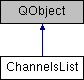
\includegraphics[height=2.000000cm]{class_channels_list}
\end{center}
\end{figure}
\subsection*{Signals}
\begin{DoxyCompactItemize}
\item 
void \textbf{ namechanged} (Q\+String, int)
\end{DoxyCompactItemize}
\subsection*{Public Member Functions}
\begin{DoxyCompactItemize}
\item 
\textbf{ Channels\+List} (Q\+Widget $\ast$\textbf{ framework}, int number, bool \textbf{ showdevices})
\begin{DoxyCompactList}\small\item\em \doxyref{Channels\+List}{p.}{class_channels_list} constructor. \end{DoxyCompactList}\item 
\textbf{ $\sim$\+Channels\+List} ()
\begin{DoxyCompactList}\small\item\em \doxyref{Channels\+List}{p.}{class_channels_list} destructor. \end{DoxyCompactList}\item 
\textbf{ Channel} $\ast$ \textbf{ get\+Channel} (int index)
\begin{DoxyCompactList}\small\item\em It gets a channel. \end{DoxyCompactList}\item 
void \textbf{ delete\+Channel} (int index)
\begin{DoxyCompactList}\small\item\em It deletes a channel. \end{DoxyCompactList}\item 
int \textbf{ get\+Size} ()
\begin{DoxyCompactList}\small\item\em It gets the number of channels. \end{DoxyCompactList}\item 
void \textbf{ set\+Size} (int size)
\begin{DoxyCompactList}\small\item\em It sets a number of channels up. \end{DoxyCompactList}\item 
std\+::vector$<$ std\+::string $>$ \textbf{ get\+Names} ()
\begin{DoxyCompactList}\small\item\em It gets all channels names. \end{DoxyCompactList}\end{DoxyCompactItemize}
\subsection*{Static Public Attributes}
\begin{DoxyCompactItemize}
\item 
static int \textbf{ fs}
\item 
static int \textbf{ samplesize}
\end{DoxyCompactItemize}
\subsection*{Private Slots}
\begin{Indent}\textbf{ Channels interface slots}\par
{\em User interface control functions of channels list. }\begin{DoxyCompactItemize}
\item 
void \textbf{ set\+Label} (Q\+String label)
\begin{DoxyCompactList}\small\item\em Slot for setting the channel label. \end{DoxyCompactList}\item 
void \textbf{ set\+Label} (Q\+String label, int index)
\begin{DoxyCompactList}\small\item\em Slot for setting the channel label. \end{DoxyCompactList}\item 
void \textbf{ set\+Volume} (int volume)
\begin{DoxyCompactList}\small\item\em Slots for setting the channel level. \end{DoxyCompactList}\item 
void \textbf{ mute} (bool state)
\begin{DoxyCompactList}\small\item\em Slots when muted checkbox has been changed. \end{DoxyCompactList}\item 
void \textbf{ bypass} (bool state)
\begin{DoxyCompactList}\small\item\em Slots when muted checkbox has been changed. \end{DoxyCompactList}\item 
void \textbf{ set\+Device} (int device)
\begin{DoxyCompactList}\small\item\em Slots for setting an audio output device. \end{DoxyCompactList}\end{DoxyCompactItemize}
\end{Indent}
\subsection*{Private Member Functions}
\begin{DoxyCompactItemize}
\item 
int \textbf{ get\+Index} (Q\+Object $\ast$element)
\begin{DoxyCompactList}\small\item\em It gets the channel index of a user interface element. \end{DoxyCompactList}\end{DoxyCompactItemize}
\subsection*{Private Attributes}
\begin{DoxyCompactItemize}
\item 
std\+::vector$<$ \textbf{ Channel} $\ast$ $>$ \textbf{ channels}
\item 
std\+::string \textbf{ prefix}
\item 
bool \textbf{ showdevices}
\item 
Q\+Widget $\ast$ \textbf{ framework}
\item 
Q\+Layout $\ast$ \textbf{ layout}
\end{DoxyCompactItemize}


\subsection{Detailed Description}
Channels list class. It shows information about channels signals. 

\begin{DoxyAuthor}{Author}
Andrés González Fornell 
\end{DoxyAuthor}


\subsection{Constructor \& Destructor Documentation}
\mbox{\label{class_channels_list_a2be2b5b850d9841fc90208afc7c6f112}} 
\index{Channels\+List@{Channels\+List}!Channels\+List@{Channels\+List}}
\index{Channels\+List@{Channels\+List}!Channels\+List@{Channels\+List}}
\subsubsection{Channels\+List()}
{\footnotesize\ttfamily Channels\+List\+::\+Channels\+List (\begin{DoxyParamCaption}\item[{Q\+Widget $\ast$}]{framework,  }\item[{int}]{number,  }\item[{bool}]{showdevices }\end{DoxyParamCaption})}



\doxyref{Channels\+List}{p.}{class_channels_list} constructor. 


\begin{DoxyParams}{Parameters}
{\em framework} & user interface framework of channels list \\
\hline
{\em number} & number of channels \\
\hline
{\em showdevices} & true to create device selector to send audio to the system audio output devices \\
\hline
\end{DoxyParams}
\mbox{\label{class_channels_list_a264a8cdd2dc552462b1de06ec02729ec}} 
\index{Channels\+List@{Channels\+List}!````~Channels\+List@{$\sim$\+Channels\+List}}
\index{````~Channels\+List@{$\sim$\+Channels\+List}!Channels\+List@{Channels\+List}}
\subsubsection{$\sim$\+Channels\+List()}
{\footnotesize\ttfamily Channels\+List\+::$\sim$\+Channels\+List (\begin{DoxyParamCaption}{ }\end{DoxyParamCaption})}



\doxyref{Channels\+List}{p.}{class_channels_list} destructor. 



\subsection{Member Function Documentation}
\mbox{\label{class_channels_list_a95eca3eefbcf94fa4c7a3d3af3941319}} 
\index{Channels\+List@{Channels\+List}!bypass@{bypass}}
\index{bypass@{bypass}!Channels\+List@{Channels\+List}}
\subsubsection{bypass}
{\footnotesize\ttfamily void Channels\+List\+::bypass (\begin{DoxyParamCaption}\item[{bool}]{state }\end{DoxyParamCaption})\hspace{0.3cm}{\ttfamily [private]}, {\ttfamily [slot]}}



Slots when muted checkbox has been changed. 


\begin{DoxyParams}{Parameters}
{\em state} & current checkbox state \\
\hline
\end{DoxyParams}
\mbox{\label{class_channels_list_a72dfd281e40fd29624354254ad3fa791}} 
\index{Channels\+List@{Channels\+List}!delete\+Channel@{delete\+Channel}}
\index{delete\+Channel@{delete\+Channel}!Channels\+List@{Channels\+List}}
\subsubsection{delete\+Channel()}
{\footnotesize\ttfamily void Channels\+List\+::delete\+Channel (\begin{DoxyParamCaption}\item[{int}]{index }\end{DoxyParamCaption})}



It deletes a channel. 


\begin{DoxyParams}{Parameters}
{\em index} & channel index \\
\hline
\end{DoxyParams}
\mbox{\label{class_channels_list_a794574bee033fd0fa2bee54c615576f9}} 
\index{Channels\+List@{Channels\+List}!get\+Channel@{get\+Channel}}
\index{get\+Channel@{get\+Channel}!Channels\+List@{Channels\+List}}
\subsubsection{get\+Channel()}
{\footnotesize\ttfamily \textbf{ Channel} $\ast$ Channels\+List\+::get\+Channel (\begin{DoxyParamCaption}\item[{int}]{index }\end{DoxyParamCaption})}



It gets a channel. 


\begin{DoxyParams}{Parameters}
{\em index} & channel index \\
\hline
\end{DoxyParams}
\begin{DoxyReturn}{Returns}
channel pointer 
\end{DoxyReturn}
\mbox{\label{class_channels_list_a47e6b8432656134624e311f6a16da67d}} 
\index{Channels\+List@{Channels\+List}!get\+Index@{get\+Index}}
\index{get\+Index@{get\+Index}!Channels\+List@{Channels\+List}}
\subsubsection{get\+Index()}
{\footnotesize\ttfamily int Channels\+List\+::get\+Index (\begin{DoxyParamCaption}\item[{Q\+Object $\ast$}]{element }\end{DoxyParamCaption})\hspace{0.3cm}{\ttfamily [private]}}



It gets the channel index of a user interface element. 


\begin{DoxyParams}{Parameters}
{\em element} & user interface element \\
\hline
\end{DoxyParams}
\begin{DoxyReturn}{Returns}
index 
\end{DoxyReturn}
\mbox{\label{class_channels_list_a17482d918a0dbbd4bf0fc2a22ee67668}} 
\index{Channels\+List@{Channels\+List}!get\+Names@{get\+Names}}
\index{get\+Names@{get\+Names}!Channels\+List@{Channels\+List}}
\subsubsection{get\+Names()}
{\footnotesize\ttfamily std\+::vector$<$ std\+::string $>$ Channels\+List\+::get\+Names (\begin{DoxyParamCaption}{ }\end{DoxyParamCaption})}



It gets all channels names. 

\begin{DoxyReturn}{Returns}
list of channels names 
\end{DoxyReturn}
\mbox{\label{class_channels_list_aeaeb08c6bf8aa1a48b5cc52c56505408}} 
\index{Channels\+List@{Channels\+List}!get\+Size@{get\+Size}}
\index{get\+Size@{get\+Size}!Channels\+List@{Channels\+List}}
\subsubsection{get\+Size()}
{\footnotesize\ttfamily int Channels\+List\+::get\+Size (\begin{DoxyParamCaption}{ }\end{DoxyParamCaption})}



It gets the number of channels. 

\begin{DoxyReturn}{Returns}
number of channels 
\end{DoxyReturn}
\mbox{\label{class_channels_list_adeed14dbeece6de23be83bfb6e7ab680}} 
\index{Channels\+List@{Channels\+List}!mute@{mute}}
\index{mute@{mute}!Channels\+List@{Channels\+List}}
\subsubsection{mute}
{\footnotesize\ttfamily void Channels\+List\+::mute (\begin{DoxyParamCaption}\item[{bool}]{state }\end{DoxyParamCaption})\hspace{0.3cm}{\ttfamily [private]}, {\ttfamily [slot]}}



Slots when muted checkbox has been changed. 


\begin{DoxyParams}{Parameters}
{\em state} & current checkbox state \\
\hline
\end{DoxyParams}
\mbox{\label{class_channels_list_a78d7e060309b406ad27f4abf148e76d0}} 
\index{Channels\+List@{Channels\+List}!namechanged@{namechanged}}
\index{namechanged@{namechanged}!Channels\+List@{Channels\+List}}
\subsubsection{namechanged}
{\footnotesize\ttfamily void Channels\+List\+::namechanged (\begin{DoxyParamCaption}\item[{Q\+String}]{,  }\item[{int}]{ }\end{DoxyParamCaption})\hspace{0.3cm}{\ttfamily [signal]}}

\mbox{\label{class_channels_list_ae1edf65c94deca2a3911d11a9b96cd8e}} 
\index{Channels\+List@{Channels\+List}!set\+Device@{set\+Device}}
\index{set\+Device@{set\+Device}!Channels\+List@{Channels\+List}}
\subsubsection{set\+Device}
{\footnotesize\ttfamily void Channels\+List\+::set\+Device (\begin{DoxyParamCaption}\item[{int}]{device }\end{DoxyParamCaption})\hspace{0.3cm}{\ttfamily [private]}, {\ttfamily [slot]}}



Slots for setting an audio output device. 


\begin{DoxyParams}{Parameters}
{\em device} & device index \\
\hline
\end{DoxyParams}
\mbox{\label{class_channels_list_adc787dbb51d4e2d2c733d53f4ee293fa}} 
\index{Channels\+List@{Channels\+List}!set\+Label@{set\+Label}}
\index{set\+Label@{set\+Label}!Channels\+List@{Channels\+List}}
\subsubsection{set\+Label\hspace{0.1cm}{\footnotesize\ttfamily [1/2]}}
{\footnotesize\ttfamily void Channels\+List\+::set\+Label (\begin{DoxyParamCaption}\item[{Q\+String}]{label }\end{DoxyParamCaption})\hspace{0.3cm}{\ttfamily [private]}, {\ttfamily [slot]}}



Slot for setting the channel label. 


\begin{DoxyParams}{Parameters}
{\em label} & \\
\hline
\end{DoxyParams}
\mbox{\label{class_channels_list_ad1f939c83b4444269d130dcb5569133f}} 
\index{Channels\+List@{Channels\+List}!set\+Label@{set\+Label}}
\index{set\+Label@{set\+Label}!Channels\+List@{Channels\+List}}
\subsubsection{set\+Label\hspace{0.1cm}{\footnotesize\ttfamily [2/2]}}
{\footnotesize\ttfamily void Channels\+List\+::set\+Label (\begin{DoxyParamCaption}\item[{Q\+String}]{label,  }\item[{int}]{index }\end{DoxyParamCaption})\hspace{0.3cm}{\ttfamily [private]}, {\ttfamily [slot]}}



Slot for setting the channel label. 


\begin{DoxyParams}{Parameters}
{\em label} & \\
\hline
{\em index} & channel index \\
\hline
\end{DoxyParams}
\mbox{\label{class_channels_list_ac059e3c89763f50705ce1e2633ee3d3d}} 
\index{Channels\+List@{Channels\+List}!set\+Size@{set\+Size}}
\index{set\+Size@{set\+Size}!Channels\+List@{Channels\+List}}
\subsubsection{set\+Size()}
{\footnotesize\ttfamily void Channels\+List\+::set\+Size (\begin{DoxyParamCaption}\item[{int}]{size }\end{DoxyParamCaption})}



It sets a number of channels up. 


\begin{DoxyParams}{Parameters}
{\em size} & number of channels \\
\hline
\end{DoxyParams}
\mbox{\label{class_channels_list_adbc31fe3486c8a6aa3302a1c226ca60a}} 
\index{Channels\+List@{Channels\+List}!set\+Volume@{set\+Volume}}
\index{set\+Volume@{set\+Volume}!Channels\+List@{Channels\+List}}
\subsubsection{set\+Volume}
{\footnotesize\ttfamily void Channels\+List\+::set\+Volume (\begin{DoxyParamCaption}\item[{int}]{volume }\end{DoxyParamCaption})\hspace{0.3cm}{\ttfamily [private]}, {\ttfamily [slot]}}



Slots for setting the channel level. 


\begin{DoxyParams}{Parameters}
{\em volume} & integer number from 0 to 100 \\
\hline
\end{DoxyParams}


\subsection{Member Data Documentation}
\mbox{\label{class_channels_list_aada1aa2e93c00e98776ca02f4ba37807}} 
\index{Channels\+List@{Channels\+List}!channels@{channels}}
\index{channels@{channels}!Channels\+List@{Channels\+List}}
\subsubsection{channels}
{\footnotesize\ttfamily std\+::vector$<$\textbf{ Channel} $\ast$$>$ Channels\+List\+::channels\hspace{0.3cm}{\ttfamily [private]}}

list of channels \mbox{\label{class_channels_list_a95ce83d3108c23dacd899ff33e43e6f5}} 
\index{Channels\+List@{Channels\+List}!framework@{framework}}
\index{framework@{framework}!Channels\+List@{Channels\+List}}
\subsubsection{framework}
{\footnotesize\ttfamily Q\+Widget$\ast$ Channels\+List\+::framework\hspace{0.3cm}{\ttfamily [private]}}

user interface framework of channels list \mbox{\label{class_channels_list_ab5b3fd699a6c96a59d237ff4e23fa3fa}} 
\index{Channels\+List@{Channels\+List}!fs@{fs}}
\index{fs@{fs}!Channels\+List@{Channels\+List}}
\subsubsection{fs}
{\footnotesize\ttfamily int Channels\+List\+::fs\hspace{0.3cm}{\ttfamily [static]}}

signal sampling frequency \mbox{\label{class_channels_list_adeb9c603ac2216dd014b723a326f0c62}} 
\index{Channels\+List@{Channels\+List}!layout@{layout}}
\index{layout@{layout}!Channels\+List@{Channels\+List}}
\subsubsection{layout}
{\footnotesize\ttfamily Q\+Layout$\ast$ Channels\+List\+::layout\hspace{0.3cm}{\ttfamily [private]}}

user interface layout of channels list \mbox{\label{class_channels_list_a452e6090d13b327758ae0e3992ed620c}} 
\index{Channels\+List@{Channels\+List}!prefix@{prefix}}
\index{prefix@{prefix}!Channels\+List@{Channels\+List}}
\subsubsection{prefix}
{\footnotesize\ttfamily std\+::string Channels\+List\+::prefix\hspace{0.3cm}{\ttfamily [private]}}

user interface prefix \mbox{\label{class_channels_list_ac9208b24e03fac37e06e9664ed26b13b}} 
\index{Channels\+List@{Channels\+List}!samplesize@{samplesize}}
\index{samplesize@{samplesize}!Channels\+List@{Channels\+List}}
\subsubsection{samplesize}
{\footnotesize\ttfamily int Channels\+List\+::samplesize\hspace{0.3cm}{\ttfamily [static]}}

signal sample size \mbox{\label{class_channels_list_ac5467a8384f559129cc71c31a6c95972}} 
\index{Channels\+List@{Channels\+List}!showdevices@{showdevices}}
\index{showdevices@{showdevices}!Channels\+List@{Channels\+List}}
\subsubsection{showdevices}
{\footnotesize\ttfamily bool Channels\+List\+::showdevices\hspace{0.3cm}{\ttfamily [private]}}

true to show audio output device selector (in case of sending channels to speakers or other audio output system devices) 

The documentation for this class was generated from the following files\+:\begin{DoxyCompactItemize}
\item 
src/interface/\textbf{ Channels\+List.\+h}\item 
src/interface/\textbf{ Channels\+List.\+cpp}\item 
src/interface/\textbf{ S\+A\+C\+Effects.\+cpp}\end{DoxyCompactItemize}

\hypertarget{struct_s_a_c_bitstream_1_1_channel_type}{}\section{S\+A\+C\+Bitstream\+:\+:Channel\+Type Struct Reference}
\label{struct_s_a_c_bitstream_1_1_channel_type}\index{S\+A\+C\+Bitstream\+::\+Channel\+Type@{S\+A\+C\+Bitstream\+::\+Channel\+Type}}


It specifies the channel type.  




{\ttfamily \#include $<$S\+A\+C\+Bitstream.\+h$>$}

\subsection*{Public Types}
\begin{DoxyCompactItemize}
\item 
enum \hyperlink{struct_s_a_c_bitstream_1_1_channel_type_a31c32b34085c06a1c58d920ca28c17c9}{channeltype} \{ \newline
\hyperlink{struct_s_a_c_bitstream_1_1_channel_type_a31c32b34085c06a1c58d920ca28c17c9a13eb8514591dc8f914e828a2b5ef721a}{L} = 0x0, 
\hyperlink{struct_s_a_c_bitstream_1_1_channel_type_a31c32b34085c06a1c58d920ca28c17c9ad134acdd72d975dd185adc12af56fbdd}{Lc} = 0x1, 
\hyperlink{struct_s_a_c_bitstream_1_1_channel_type_a31c32b34085c06a1c58d920ca28c17c9abfabd18311453175371708dbc80ae9fa}{Ls} = 0x2, 
\hyperlink{struct_s_a_c_bitstream_1_1_channel_type_a31c32b34085c06a1c58d920ca28c17c9a723885ae87caa2993f734cda066c93c8}{Lsr} = 0x3, 
\newline
\hyperlink{struct_s_a_c_bitstream_1_1_channel_type_a31c32b34085c06a1c58d920ca28c17c9a464953c6afaf1a65f4e7fbeba29c6049}{R} = 0x4, 
\hyperlink{struct_s_a_c_bitstream_1_1_channel_type_a31c32b34085c06a1c58d920ca28c17c9abb6f27e48c485d4c40f2fb4035c033ca}{Rc} = 0x5, 
\hyperlink{struct_s_a_c_bitstream_1_1_channel_type_a31c32b34085c06a1c58d920ca28c17c9a58602376d8c460fe2b26af6b4eb7c837}{Rs} = 0x6, 
\hyperlink{struct_s_a_c_bitstream_1_1_channel_type_a31c32b34085c06a1c58d920ca28c17c9a3fa09df79b849c2f632473b2380ad07e}{Rsr} = 0x7, 
\newline
\hyperlink{struct_s_a_c_bitstream_1_1_channel_type_a31c32b34085c06a1c58d920ca28c17c9a5c9b81e6c191dc59f0f4680421cafa72}{C} = 0x8, 
\hyperlink{struct_s_a_c_bitstream_1_1_channel_type_a31c32b34085c06a1c58d920ca28c17c9a9ea1b895ad06ec34500fa5ce86f261d4}{L\+FE} = 0x9
 \}
\end{DoxyCompactItemize}


\subsection{Detailed Description}


Definition at line 21 of file S\+A\+C\+Bitstream.\+h.



\subsection{Member Enumeration Documentation}
\mbox{\Hypertarget{struct_s_a_c_bitstream_1_1_channel_type_a31c32b34085c06a1c58d920ca28c17c9}\label{struct_s_a_c_bitstream_1_1_channel_type_a31c32b34085c06a1c58d920ca28c17c9}} 
\index{S\+A\+C\+Bitstream\+::\+Channel\+Type@{S\+A\+C\+Bitstream\+::\+Channel\+Type}!channeltype@{channeltype}}
\index{channeltype@{channeltype}!S\+A\+C\+Bitstream\+::\+Channel\+Type@{S\+A\+C\+Bitstream\+::\+Channel\+Type}}
\subsubsection{\texorpdfstring{channeltype}{channeltype}}
{\footnotesize\ttfamily enum \hyperlink{struct_s_a_c_bitstream_1_1_channel_type_a31c32b34085c06a1c58d920ca28c17c9}{S\+A\+C\+Bitstream\+::\+Channel\+Type\+::channeltype}}

\begin{DoxyEnumFields}{Enumerator}
\raisebox{\heightof{T}}[0pt][0pt]{\index{L@{L}!S\+A\+C\+Bitstream\+::\+Channel\+Type@{S\+A\+C\+Bitstream\+::\+Channel\+Type}}\index{S\+A\+C\+Bitstream\+::\+Channel\+Type@{S\+A\+C\+Bitstream\+::\+Channel\+Type}!L@{L}}}\mbox{\Hypertarget{struct_s_a_c_bitstream_1_1_channel_type_a31c32b34085c06a1c58d920ca28c17c9a13eb8514591dc8f914e828a2b5ef721a}\label{struct_s_a_c_bitstream_1_1_channel_type_a31c32b34085c06a1c58d920ca28c17c9a13eb8514591dc8f914e828a2b5ef721a}} 
L&left front channel \\
\hline

\raisebox{\heightof{T}}[0pt][0pt]{\index{Lc@{Lc}!S\+A\+C\+Bitstream\+::\+Channel\+Type@{S\+A\+C\+Bitstream\+::\+Channel\+Type}}\index{S\+A\+C\+Bitstream\+::\+Channel\+Type@{S\+A\+C\+Bitstream\+::\+Channel\+Type}!Lc@{Lc}}}\mbox{\Hypertarget{struct_s_a_c_bitstream_1_1_channel_type_a31c32b34085c06a1c58d920ca28c17c9ad134acdd72d975dd185adc12af56fbdd}\label{struct_s_a_c_bitstream_1_1_channel_type_a31c32b34085c06a1c58d920ca28c17c9ad134acdd72d975dd185adc12af56fbdd}} 
Lc&left front center channel \\
\hline

\raisebox{\heightof{T}}[0pt][0pt]{\index{Ls@{Ls}!S\+A\+C\+Bitstream\+::\+Channel\+Type@{S\+A\+C\+Bitstream\+::\+Channel\+Type}}\index{S\+A\+C\+Bitstream\+::\+Channel\+Type@{S\+A\+C\+Bitstream\+::\+Channel\+Type}!Ls@{Ls}}}\mbox{\Hypertarget{struct_s_a_c_bitstream_1_1_channel_type_a31c32b34085c06a1c58d920ca28c17c9abfabd18311453175371708dbc80ae9fa}\label{struct_s_a_c_bitstream_1_1_channel_type_a31c32b34085c06a1c58d920ca28c17c9abfabd18311453175371708dbc80ae9fa}} 
Ls&left surround channel \\
\hline

\raisebox{\heightof{T}}[0pt][0pt]{\index{Lsr@{Lsr}!S\+A\+C\+Bitstream\+::\+Channel\+Type@{S\+A\+C\+Bitstream\+::\+Channel\+Type}}\index{S\+A\+C\+Bitstream\+::\+Channel\+Type@{S\+A\+C\+Bitstream\+::\+Channel\+Type}!Lsr@{Lsr}}}\mbox{\Hypertarget{struct_s_a_c_bitstream_1_1_channel_type_a31c32b34085c06a1c58d920ca28c17c9a723885ae87caa2993f734cda066c93c8}\label{struct_s_a_c_bitstream_1_1_channel_type_a31c32b34085c06a1c58d920ca28c17c9a723885ae87caa2993f734cda066c93c8}} 
Lsr&rear surround left channel \\
\hline

\raisebox{\heightof{T}}[0pt][0pt]{\index{R@{R}!S\+A\+C\+Bitstream\+::\+Channel\+Type@{S\+A\+C\+Bitstream\+::\+Channel\+Type}}\index{S\+A\+C\+Bitstream\+::\+Channel\+Type@{S\+A\+C\+Bitstream\+::\+Channel\+Type}!R@{R}}}\mbox{\Hypertarget{struct_s_a_c_bitstream_1_1_channel_type_a31c32b34085c06a1c58d920ca28c17c9a464953c6afaf1a65f4e7fbeba29c6049}\label{struct_s_a_c_bitstream_1_1_channel_type_a31c32b34085c06a1c58d920ca28c17c9a464953c6afaf1a65f4e7fbeba29c6049}} 
R&left front channel \\
\hline

\raisebox{\heightof{T}}[0pt][0pt]{\index{Rc@{Rc}!S\+A\+C\+Bitstream\+::\+Channel\+Type@{S\+A\+C\+Bitstream\+::\+Channel\+Type}}\index{S\+A\+C\+Bitstream\+::\+Channel\+Type@{S\+A\+C\+Bitstream\+::\+Channel\+Type}!Rc@{Rc}}}\mbox{\Hypertarget{struct_s_a_c_bitstream_1_1_channel_type_a31c32b34085c06a1c58d920ca28c17c9abb6f27e48c485d4c40f2fb4035c033ca}\label{struct_s_a_c_bitstream_1_1_channel_type_a31c32b34085c06a1c58d920ca28c17c9abb6f27e48c485d4c40f2fb4035c033ca}} 
Rc&left front center channel \\
\hline

\raisebox{\heightof{T}}[0pt][0pt]{\index{Rs@{Rs}!S\+A\+C\+Bitstream\+::\+Channel\+Type@{S\+A\+C\+Bitstream\+::\+Channel\+Type}}\index{S\+A\+C\+Bitstream\+::\+Channel\+Type@{S\+A\+C\+Bitstream\+::\+Channel\+Type}!Rs@{Rs}}}\mbox{\Hypertarget{struct_s_a_c_bitstream_1_1_channel_type_a31c32b34085c06a1c58d920ca28c17c9a58602376d8c460fe2b26af6b4eb7c837}\label{struct_s_a_c_bitstream_1_1_channel_type_a31c32b34085c06a1c58d920ca28c17c9a58602376d8c460fe2b26af6b4eb7c837}} 
Rs&left surround channel \\
\hline

\raisebox{\heightof{T}}[0pt][0pt]{\index{Rsr@{Rsr}!S\+A\+C\+Bitstream\+::\+Channel\+Type@{S\+A\+C\+Bitstream\+::\+Channel\+Type}}\index{S\+A\+C\+Bitstream\+::\+Channel\+Type@{S\+A\+C\+Bitstream\+::\+Channel\+Type}!Rsr@{Rsr}}}\mbox{\Hypertarget{struct_s_a_c_bitstream_1_1_channel_type_a31c32b34085c06a1c58d920ca28c17c9a3fa09df79b849c2f632473b2380ad07e}\label{struct_s_a_c_bitstream_1_1_channel_type_a31c32b34085c06a1c58d920ca28c17c9a3fa09df79b849c2f632473b2380ad07e}} 
Rsr&rear surround left channel \\
\hline

\raisebox{\heightof{T}}[0pt][0pt]{\index{C@{C}!S\+A\+C\+Bitstream\+::\+Channel\+Type@{S\+A\+C\+Bitstream\+::\+Channel\+Type}}\index{S\+A\+C\+Bitstream\+::\+Channel\+Type@{S\+A\+C\+Bitstream\+::\+Channel\+Type}!C@{C}}}\mbox{\Hypertarget{struct_s_a_c_bitstream_1_1_channel_type_a31c32b34085c06a1c58d920ca28c17c9a5c9b81e6c191dc59f0f4680421cafa72}\label{struct_s_a_c_bitstream_1_1_channel_type_a31c32b34085c06a1c58d920ca28c17c9a5c9b81e6c191dc59f0f4680421cafa72}} 
C&center front channel \\
\hline

\raisebox{\heightof{T}}[0pt][0pt]{\index{L\+FE@{L\+FE}!S\+A\+C\+Bitstream\+::\+Channel\+Type@{S\+A\+C\+Bitstream\+::\+Channel\+Type}}\index{S\+A\+C\+Bitstream\+::\+Channel\+Type@{S\+A\+C\+Bitstream\+::\+Channel\+Type}!L\+FE@{L\+FE}}}\mbox{\Hypertarget{struct_s_a_c_bitstream_1_1_channel_type_a31c32b34085c06a1c58d920ca28c17c9a9ea1b895ad06ec34500fa5ce86f261d4}\label{struct_s_a_c_bitstream_1_1_channel_type_a31c32b34085c06a1c58d920ca28c17c9a9ea1b895ad06ec34500fa5ce86f261d4}} 
L\+FE&low frequency enhancement channel \\
\hline

\end{DoxyEnumFields}


Definition at line 22 of file S\+A\+C\+Bitstream.\+h.



The documentation for this struct was generated from the following file\+:\begin{DoxyCompactItemize}
\item 
src/sac/S\+A\+C\+Bitstream.\+h\end{DoxyCompactItemize}

\hypertarget{class_chart2_d}{}\section{Chart2D Class Reference}
\label{class_chart2_d}\index{Chart2D@{Chart2D}}


Class for plotting two-\/dimensional charts.  




{\ttfamily \#include $<$Chart2\+D.\+h$>$}



Inheritance diagram for Chart2D\+:
\nopagebreak
\begin{figure}[H]
\begin{center}
\leavevmode
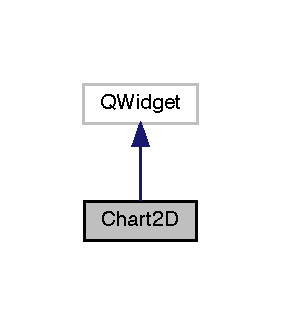
\includegraphics[width=135pt]{class_chart2_d__inherit__graph}
\end{center}
\end{figure}


Collaboration diagram for Chart2D\+:
\nopagebreak
\begin{figure}[H]
\begin{center}
\leavevmode
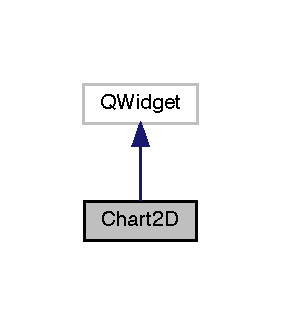
\includegraphics[width=135pt]{class_chart2_d__coll__graph}
\end{center}
\end{figure}
\subsection*{Classes}
\begin{DoxyCompactItemize}
\item 
struct \hyperlink{struct_chart2_d_1_1_chart_options}{Chart\+Options}
\begin{DoxyCompactList}\small\item\em It defines some features of the chart. \end{DoxyCompactList}\end{DoxyCompactItemize}
\subsection*{Public Member Functions}
\begin{DoxyCompactItemize}
\item 
\hyperlink{class_chart2_d_a6883ce065d3a6a52f6f72efdf35d62aa}{Chart2D} (Q\+Widget $\ast$framework)
\begin{DoxyCompactList}\small\item\em Chart constructor. \end{DoxyCompactList}\item 
\hyperlink{class_chart2_d_a4d29e59bc8eafa3267c62034b51725b4}{Chart2D} (Q\+Widget $\ast$framework, double range\mbox{[}2\mbox{]}\mbox{[}2\mbox{]}, std\+::string title, std\+::string \hyperlink{class_chart2_d_af463dc0d42e747ab4a208a44db003bd7}{xlabel}, std\+::string \hyperlink{class_chart2_d_afc4139568c9a63b3bcdc4eeefc0dd2e8}{ylabel}, int options)
\begin{DoxyCompactList}\small\item\em Chart constructor. \end{DoxyCompactList}\item 
\mbox{\Hypertarget{class_chart2_d_a73cac8978d3dd8a236ee4b2eae895a1e}\label{class_chart2_d_a73cac8978d3dd8a236ee4b2eae895a1e}} 
\hyperlink{class_chart2_d_a73cac8978d3dd8a236ee4b2eae895a1e}{$\sim$\+Chart2D} ()
\begin{DoxyCompactList}\small\item\em Chart destructor. \end{DoxyCompactList}\item 
void \hyperlink{class_chart2_d_a90db5078374163beef86536a33bbe8ba}{set\+Points} (Q\+Vector$<$ Q\+PointF $>$ points)
\begin{DoxyCompactList}\small\item\em It sets the points to the chart serie. \end{DoxyCompactList}\item 
Q\+Vector$<$ Q\+PointF $>$ \hyperlink{class_chart2_d_acbc12395c5a24b7146b8262ec2dab315}{get\+Points} ()
\begin{DoxyCompactList}\small\item\em It gets the points from the chart serie. \end{DoxyCompactList}\item 
void \hyperlink{class_chart2_d_acc60a5df11a3bb47c7888e108cd50f05}{set\+Range} (double range\mbox{[}2\mbox{]}\mbox{[}2\mbox{]})
\begin{DoxyCompactList}\small\item\em It sets the axis range. \end{DoxyCompactList}\item 
void \hyperlink{class_chart2_d_ac148952b822fcb1d0c865a7f36af85e4}{set\+Title} (std\+::string title)
\begin{DoxyCompactList}\small\item\em It sets chart title. \end{DoxyCompactList}\item 
void \hyperlink{class_chart2_d_a7a871b06da3b23bd7b452b75107132a6}{set\+Options} (int options)
\begin{DoxyCompactList}\small\item\em It sets chart options. \end{DoxyCompactList}\item 
\mbox{\Hypertarget{class_chart2_d_adc92e3ebe94275e02cf547c81d0410e9}\label{class_chart2_d_adc92e3ebe94275e02cf547c81d0410e9}} 
void \hyperlink{class_chart2_d_adc92e3ebe94275e02cf547c81d0410e9}{clear} ()
\begin{DoxyCompactList}\small\item\em It clears the chart. \end{DoxyCompactList}\end{DoxyCompactItemize}
\subsection*{Public Attributes}
\begin{DoxyCompactItemize}
\item 
std\+::string \hyperlink{class_chart2_d_af463dc0d42e747ab4a208a44db003bd7}{xlabel}
\item 
std\+::string \hyperlink{class_chart2_d_afc4139568c9a63b3bcdc4eeefc0dd2e8}{ylabel}
\end{DoxyCompactItemize}


\subsection{Detailed Description}
\begin{DoxyAuthor}{Author}
Andrés González Fornell 
\end{DoxyAuthor}


Definition at line 22 of file Chart2\+D.\+h.



\subsection{Constructor \& Destructor Documentation}
\mbox{\Hypertarget{class_chart2_d_a6883ce065d3a6a52f6f72efdf35d62aa}\label{class_chart2_d_a6883ce065d3a6a52f6f72efdf35d62aa}} 
\index{Chart2D@{Chart2D}!Chart2D@{Chart2D}}
\index{Chart2D@{Chart2D}!Chart2D@{Chart2D}}
\subsubsection{\texorpdfstring{Chart2\+D()}{Chart2D()}\hspace{0.1cm}{\footnotesize\ttfamily [1/2]}}
{\footnotesize\ttfamily Chart2\+D\+::\+Chart2D (\begin{DoxyParamCaption}\item[{Q\+Widget $\ast$}]{framework }\end{DoxyParamCaption})}


\begin{DoxyParams}{Parameters}
{\em framework} & user interface framework of chart \\
\hline
\end{DoxyParams}


Definition at line 8 of file Chart2\+D.\+cpp.

Here is the call graph for this function\+:
\nopagebreak
\begin{figure}[H]
\begin{center}
\leavevmode
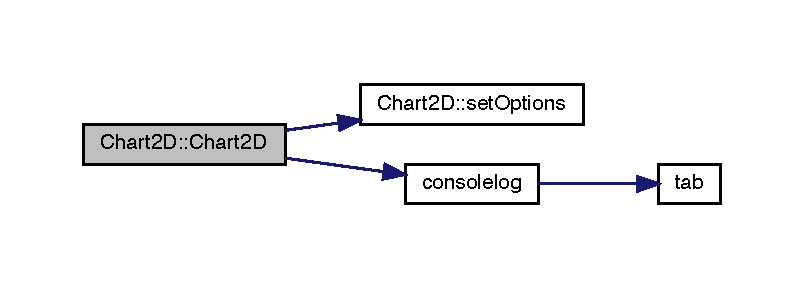
\includegraphics[width=350pt]{class_chart2_d_a6883ce065d3a6a52f6f72efdf35d62aa_cgraph}
\end{center}
\end{figure}
\mbox{\Hypertarget{class_chart2_d_a4d29e59bc8eafa3267c62034b51725b4}\label{class_chart2_d_a4d29e59bc8eafa3267c62034b51725b4}} 
\index{Chart2D@{Chart2D}!Chart2D@{Chart2D}}
\index{Chart2D@{Chart2D}!Chart2D@{Chart2D}}
\subsubsection{\texorpdfstring{Chart2\+D()}{Chart2D()}\hspace{0.1cm}{\footnotesize\ttfamily [2/2]}}
{\footnotesize\ttfamily Chart2\+D\+::\+Chart2D (\begin{DoxyParamCaption}\item[{Q\+Widget $\ast$}]{framework,  }\item[{double}]{range\mbox{[}2\mbox{]}\mbox{[}2\mbox{]},  }\item[{std\+::string}]{title,  }\item[{std\+::string}]{xlabel,  }\item[{std\+::string}]{ylabel,  }\item[{int}]{options }\end{DoxyParamCaption})}


\begin{DoxyParams}{Parameters}
{\em framework} & user interface framework of chart \\
\hline
{\em range} & axes range matrix (range\mbox{[}0\mbox{]}\mbox{[}0\mbox{]} = x\+\_\+min, range\mbox{[}0\mbox{]}\mbox{[}1\mbox{]} = x\+\_\+max, range\mbox{[}1\mbox{]}\mbox{[}0\mbox{]} = y\+\_\+min, range\mbox{[}1\mbox{]}\mbox{[}1\mbox{]} = y\+\_\+max) \\
\hline
{\em title} & chart title (it will be impress on the chart) \\
\hline
{\em xlabel} & label for horizontal (x) axis \\
\hline
{\em ylabel} & label for vertical (y) axis \\
\hline
{\em options} & \hyperlink{struct_chart2_d_1_1_chart_options}{Chart\+Options} \\
\hline
\end{DoxyParams}


Definition at line 31 of file Chart2\+D.\+cpp.

Here is the call graph for this function\+:
\nopagebreak
\begin{figure}[H]
\begin{center}
\leavevmode
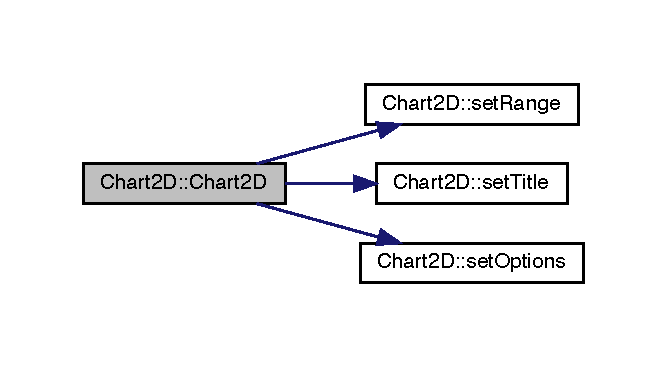
\includegraphics[width=320pt]{class_chart2_d_a4d29e59bc8eafa3267c62034b51725b4_cgraph}
\end{center}
\end{figure}


\subsection{Member Function Documentation}
\mbox{\Hypertarget{class_chart2_d_acbc12395c5a24b7146b8262ec2dab315}\label{class_chart2_d_acbc12395c5a24b7146b8262ec2dab315}} 
\index{Chart2D@{Chart2D}!get\+Points@{get\+Points}}
\index{get\+Points@{get\+Points}!Chart2D@{Chart2D}}
\subsubsection{\texorpdfstring{get\+Points()}{getPoints()}}
{\footnotesize\ttfamily Q\+Vector$<$ Q\+PointF $>$ Chart2\+D\+::get\+Points (\begin{DoxyParamCaption}{ }\end{DoxyParamCaption})}

\begin{DoxyReturn}{Returns}
points chart points 
\end{DoxyReturn}


Definition at line 60 of file Chart2\+D.\+cpp.

\mbox{\Hypertarget{class_chart2_d_a7a871b06da3b23bd7b452b75107132a6}\label{class_chart2_d_a7a871b06da3b23bd7b452b75107132a6}} 
\index{Chart2D@{Chart2D}!set\+Options@{set\+Options}}
\index{set\+Options@{set\+Options}!Chart2D@{Chart2D}}
\subsubsection{\texorpdfstring{set\+Options()}{setOptions()}}
{\footnotesize\ttfamily void Chart2\+D\+::set\+Options (\begin{DoxyParamCaption}\item[{int}]{options }\end{DoxyParamCaption})}


\begin{DoxyParams}{Parameters}
{\em options} & \hyperlink{struct_chart2_d_1_1_chart_options}{Chart\+Options} \\
\hline
\end{DoxyParams}


Definition at line 86 of file Chart2\+D.\+cpp.

Here is the caller graph for this function\+:
\nopagebreak
\begin{figure}[H]
\begin{center}
\leavevmode
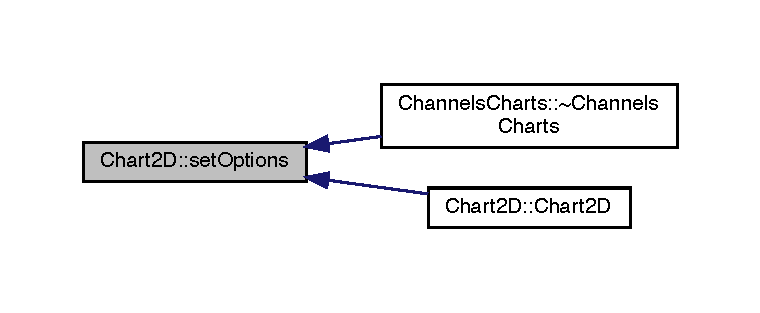
\includegraphics[width=350pt]{class_chart2_d_a7a871b06da3b23bd7b452b75107132a6_icgraph}
\end{center}
\end{figure}
\mbox{\Hypertarget{class_chart2_d_a90db5078374163beef86536a33bbe8ba}\label{class_chart2_d_a90db5078374163beef86536a33bbe8ba}} 
\index{Chart2D@{Chart2D}!set\+Points@{set\+Points}}
\index{set\+Points@{set\+Points}!Chart2D@{Chart2D}}
\subsubsection{\texorpdfstring{set\+Points()}{setPoints()}}
{\footnotesize\ttfamily void Chart2\+D\+::set\+Points (\begin{DoxyParamCaption}\item[{Q\+Vector$<$ Q\+PointF $>$}]{points }\end{DoxyParamCaption})}


\begin{DoxyParams}{Parameters}
{\em points} & new chart points \\
\hline
\end{DoxyParams}


Definition at line 52 of file Chart2\+D.\+cpp.

Here is the caller graph for this function\+:
\nopagebreak
\begin{figure}[H]
\begin{center}
\leavevmode
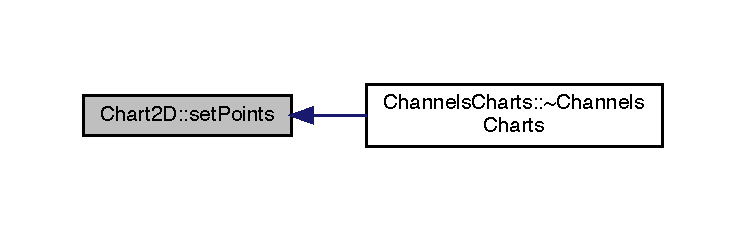
\includegraphics[width=350pt]{class_chart2_d_a90db5078374163beef86536a33bbe8ba_icgraph}
\end{center}
\end{figure}
\mbox{\Hypertarget{class_chart2_d_acc60a5df11a3bb47c7888e108cd50f05}\label{class_chart2_d_acc60a5df11a3bb47c7888e108cd50f05}} 
\index{Chart2D@{Chart2D}!set\+Range@{set\+Range}}
\index{set\+Range@{set\+Range}!Chart2D@{Chart2D}}
\subsubsection{\texorpdfstring{set\+Range()}{setRange()}}
{\footnotesize\ttfamily void Chart2\+D\+::set\+Range (\begin{DoxyParamCaption}\item[{double}]{range\mbox{[}2\mbox{]}\mbox{[}2\mbox{]} }\end{DoxyParamCaption})}


\begin{DoxyParams}{Parameters}
{\em range} & axis range matrix (range\mbox{[}0\mbox{]}\mbox{[}0\mbox{]} = x\+\_\+min, range\mbox{[}0\mbox{]}\mbox{[}1\mbox{]} = x\+\_\+max, range\mbox{[}1\mbox{]}\mbox{[}0\mbox{]} = y\+\_\+min, range\mbox{[}1\mbox{]}\mbox{[}1\mbox{]} = y\+\_\+max) \\
\hline
\end{DoxyParams}


Definition at line 68 of file Chart2\+D.\+cpp.

Here is the caller graph for this function\+:
\nopagebreak
\begin{figure}[H]
\begin{center}
\leavevmode
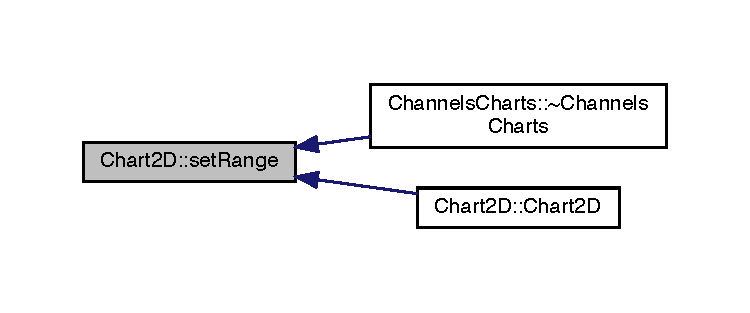
\includegraphics[width=350pt]{class_chart2_d_acc60a5df11a3bb47c7888e108cd50f05_icgraph}
\end{center}
\end{figure}
\mbox{\Hypertarget{class_chart2_d_ac148952b822fcb1d0c865a7f36af85e4}\label{class_chart2_d_ac148952b822fcb1d0c865a7f36af85e4}} 
\index{Chart2D@{Chart2D}!set\+Title@{set\+Title}}
\index{set\+Title@{set\+Title}!Chart2D@{Chart2D}}
\subsubsection{\texorpdfstring{set\+Title()}{setTitle()}}
{\footnotesize\ttfamily void Chart2\+D\+::set\+Title (\begin{DoxyParamCaption}\item[{std\+::string}]{title }\end{DoxyParamCaption})}


\begin{DoxyParams}{Parameters}
{\em title} & chart title \\
\hline
\end{DoxyParams}


Definition at line 77 of file Chart2\+D.\+cpp.

Here is the caller graph for this function\+:
\nopagebreak
\begin{figure}[H]
\begin{center}
\leavevmode
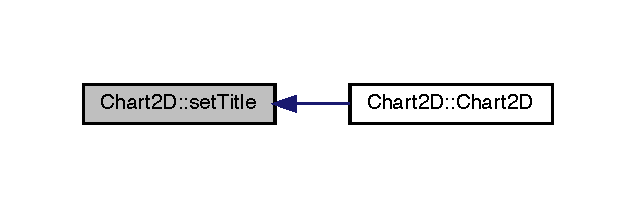
\includegraphics[width=305pt]{class_chart2_d_ac148952b822fcb1d0c865a7f36af85e4_icgraph}
\end{center}
\end{figure}


\subsection{Member Data Documentation}
\mbox{\Hypertarget{class_chart2_d_af463dc0d42e747ab4a208a44db003bd7}\label{class_chart2_d_af463dc0d42e747ab4a208a44db003bd7}} 
\index{Chart2D@{Chart2D}!xlabel@{xlabel}}
\index{xlabel@{xlabel}!Chart2D@{Chart2D}}
\subsubsection{\texorpdfstring{xlabel}{xlabel}}
{\footnotesize\ttfamily std\+::string Chart2\+D\+::xlabel}

horizontal (x) axis label 

Definition at line 37 of file Chart2\+D.\+h.

\mbox{\Hypertarget{class_chart2_d_afc4139568c9a63b3bcdc4eeefc0dd2e8}\label{class_chart2_d_afc4139568c9a63b3bcdc4eeefc0dd2e8}} 
\index{Chart2D@{Chart2D}!ylabel@{ylabel}}
\index{ylabel@{ylabel}!Chart2D@{Chart2D}}
\subsubsection{\texorpdfstring{ylabel}{ylabel}}
{\footnotesize\ttfamily std\+::string Chart2\+D\+::ylabel}

vertical (y) axis label 

Definition at line 38 of file Chart2\+D.\+h.



The documentation for this class was generated from the following files\+:\begin{DoxyCompactItemize}
\item 
src/interface/Chart2\+D.\+h\item 
src/interface/Chart2\+D.\+cpp\end{DoxyCompactItemize}

\hypertarget{struct_chart2_d_1_1_chart_options}{}\section{Chart2D\+:\+:Chart\+Options Struct Reference}
\label{struct_chart2_d_1_1_chart_options}\index{Chart2\+D\+::\+Chart\+Options@{Chart2\+D\+::\+Chart\+Options}}


It defines some features of the chart.  




{\ttfamily \#include $<$Chart2\+D.\+h$>$}

\subsection*{Public Types}
\begin{DoxyCompactItemize}
\item 
enum \hyperlink{struct_chart2_d_1_1_chart_options_a796006d22e811fc736d9cf4fb38f6b69}{Options} \{ \newline
\hyperlink{struct_chart2_d_1_1_chart_options_a796006d22e811fc736d9cf4fb38f6b69ac51488678d517feb63825d59ab9acfb1}{logX} = 0x00001, 
\hyperlink{struct_chart2_d_1_1_chart_options_a796006d22e811fc736d9cf4fb38f6b69af9bd258ed39b48502e9bbd0df9c6316c}{logY} = 0x00010, 
\hyperlink{struct_chart2_d_1_1_chart_options_a796006d22e811fc736d9cf4fb38f6b69a20ef332f00d99607527d9ca2a24a7ce9}{labelX} = 0x00100, 
\hyperlink{struct_chart2_d_1_1_chart_options_a796006d22e811fc736d9cf4fb38f6b69a003f8c6d93caf26f4d3160cfdf9e7f76}{labelY} = 0x01000, 
\newline
\hyperlink{struct_chart2_d_1_1_chart_options_a796006d22e811fc736d9cf4fb38f6b69abe6091aa82c65558fdb1cadaa45aec39}{legend} = 0x10000
 \}
\end{DoxyCompactItemize}


\subsection{Detailed Description}


Definition at line 28 of file Chart2\+D.\+h.



\subsection{Member Enumeration Documentation}
\mbox{\Hypertarget{struct_chart2_d_1_1_chart_options_a796006d22e811fc736d9cf4fb38f6b69}\label{struct_chart2_d_1_1_chart_options_a796006d22e811fc736d9cf4fb38f6b69}} 
\index{Chart2\+D\+::\+Chart\+Options@{Chart2\+D\+::\+Chart\+Options}!Options@{Options}}
\index{Options@{Options}!Chart2\+D\+::\+Chart\+Options@{Chart2\+D\+::\+Chart\+Options}}
\subsubsection{\texorpdfstring{Options}{Options}}
{\footnotesize\ttfamily enum \hyperlink{struct_chart2_d_1_1_chart_options_a796006d22e811fc736d9cf4fb38f6b69}{Chart2\+D\+::\+Chart\+Options\+::\+Options}}

\begin{DoxyEnumFields}{Enumerator}
\raisebox{\heightof{T}}[0pt][0pt]{\index{logX@{logX}!Chart2\+D\+::\+Chart\+Options@{Chart2\+D\+::\+Chart\+Options}}\index{Chart2\+D\+::\+Chart\+Options@{Chart2\+D\+::\+Chart\+Options}!logX@{logX}}}\mbox{\Hypertarget{struct_chart2_d_1_1_chart_options_a796006d22e811fc736d9cf4fb38f6b69ac51488678d517feb63825d59ab9acfb1}\label{struct_chart2_d_1_1_chart_options_a796006d22e811fc736d9cf4fb38f6b69ac51488678d517feb63825d59ab9acfb1}} 
logX&it configures the x axis as logarithm scale \\
\hline

\raisebox{\heightof{T}}[0pt][0pt]{\index{logY@{logY}!Chart2\+D\+::\+Chart\+Options@{Chart2\+D\+::\+Chart\+Options}}\index{Chart2\+D\+::\+Chart\+Options@{Chart2\+D\+::\+Chart\+Options}!logY@{logY}}}\mbox{\Hypertarget{struct_chart2_d_1_1_chart_options_a796006d22e811fc736d9cf4fb38f6b69af9bd258ed39b48502e9bbd0df9c6316c}\label{struct_chart2_d_1_1_chart_options_a796006d22e811fc736d9cf4fb38f6b69af9bd258ed39b48502e9bbd0df9c6316c}} 
logY&it configures the y axis as logarithm scale \\
\hline

\raisebox{\heightof{T}}[0pt][0pt]{\index{labelX@{labelX}!Chart2\+D\+::\+Chart\+Options@{Chart2\+D\+::\+Chart\+Options}}\index{Chart2\+D\+::\+Chart\+Options@{Chart2\+D\+::\+Chart\+Options}!labelX@{labelX}}}\mbox{\Hypertarget{struct_chart2_d_1_1_chart_options_a796006d22e811fc736d9cf4fb38f6b69a20ef332f00d99607527d9ca2a24a7ce9}\label{struct_chart2_d_1_1_chart_options_a796006d22e811fc736d9cf4fb38f6b69a20ef332f00d99607527d9ca2a24a7ce9}} 
labelX&it shows the x axis description on the chart \\
\hline

\raisebox{\heightof{T}}[0pt][0pt]{\index{labelY@{labelY}!Chart2\+D\+::\+Chart\+Options@{Chart2\+D\+::\+Chart\+Options}}\index{Chart2\+D\+::\+Chart\+Options@{Chart2\+D\+::\+Chart\+Options}!labelY@{labelY}}}\mbox{\Hypertarget{struct_chart2_d_1_1_chart_options_a796006d22e811fc736d9cf4fb38f6b69a003f8c6d93caf26f4d3160cfdf9e7f76}\label{struct_chart2_d_1_1_chart_options_a796006d22e811fc736d9cf4fb38f6b69a003f8c6d93caf26f4d3160cfdf9e7f76}} 
labelY&it shows the y axis description on the chart \\
\hline

\raisebox{\heightof{T}}[0pt][0pt]{\index{legend@{legend}!Chart2\+D\+::\+Chart\+Options@{Chart2\+D\+::\+Chart\+Options}}\index{Chart2\+D\+::\+Chart\+Options@{Chart2\+D\+::\+Chart\+Options}!legend@{legend}}}\mbox{\Hypertarget{struct_chart2_d_1_1_chart_options_a796006d22e811fc736d9cf4fb38f6b69abe6091aa82c65558fdb1cadaa45aec39}\label{struct_chart2_d_1_1_chart_options_a796006d22e811fc736d9cf4fb38f6b69abe6091aa82c65558fdb1cadaa45aec39}} 
legend&it shows the legend on the chart \\
\hline

\end{DoxyEnumFields}


Definition at line 29 of file Chart2\+D.\+h.



The documentation for this struct was generated from the following file\+:\begin{DoxyCompactItemize}
\item 
src/interface/Chart2\+D.\+h\end{DoxyCompactItemize}

\section{Compressor Class Reference}
\label{class_compressor}\index{Compressor@{Compressor}}


Audio compressor.  




{\ttfamily \#include $<$Compressor.\+h$>$}



\subsection{Detailed Description}
Audio compressor. 

\begin{DoxyAuthor}{Author}
Andrés González Fornell 
\end{DoxyAuthor}


The documentation for this class was generated from the following file\+:\begin{DoxyCompactItemize}
\item 
src/effects/\textbf{ Compressor.\+h}\end{DoxyCompactItemize}

\section{Decoding\+Type Struct Reference}
\label{struct_decoding_type}\index{Decoding\+Type@{Decoding\+Type}}


S\+AC decoder parameter decoding type.  




{\ttfamily \#include $<$S\+A\+C\+Effects.\+h$>$}

\subsection*{Public Types}
\begin{DoxyCompactItemize}
\item 
enum \textbf{ decodingtype} \{ \textbf{ low} = 0, 
\textbf{ high} = 1
 \}
\end{DoxyCompactItemize}


\subsection{Detailed Description}
S\+AC decoder parameter decoding type. 

\subsection{Member Enumeration Documentation}
\mbox{\label{struct_decoding_type_a8b3854652406458753c9b7da2068b822}} 
\index{Decoding\+Type@{Decoding\+Type}!decodingtype@{decodingtype}}
\index{decodingtype@{decodingtype}!Decoding\+Type@{Decoding\+Type}}
\subsubsection{decodingtype}
{\footnotesize\ttfamily enum \textbf{ Decoding\+Type\+::decodingtype}}

\begin{DoxyEnumFields}{Enumerator}
\raisebox{\heightof{T}}[0pt][0pt]{\index{low@{low}!Decoding\+Type@{Decoding\+Type}}\index{Decoding\+Type@{Decoding\+Type}!low@{low}}}\mbox{\label{struct_decoding_type_a8b3854652406458753c9b7da2068b822a1c83062a65b39a734cfb6393fa679425}} 
low&\\
\hline

\raisebox{\heightof{T}}[0pt][0pt]{\index{high@{high}!Decoding\+Type@{Decoding\+Type}}\index{Decoding\+Type@{Decoding\+Type}!high@{high}}}\mbox{\label{struct_decoding_type_a8b3854652406458753c9b7da2068b822a6184aedf8f82a070f5c054ead79d4d30}} 
high&\\
\hline

\end{DoxyEnumFields}


The documentation for this struct was generated from the following file\+:\begin{DoxyCompactItemize}
\item 
src/interface/\textbf{ S\+A\+C\+Effects.\+h}\end{DoxyCompactItemize}

\hypertarget{class_effect}{}\section{Effect Class Reference}
\label{class_effect}\index{Effect@{Effect}}


\hyperlink{class_effect}{Effect} class. It contains (by inheritance) all effects classes.  




{\ttfamily \#include $<$Effect.\+h$>$}

\subsection*{Public Types}
\begin{DoxyCompactItemize}
\item 
enum \hyperlink{class_effect_a6422fe21e9e452943fbc3344884a6fed}{effect\+ID} \{ \hyperlink{class_effect_a6422fe21e9e452943fbc3344884a6fedae2be861676276fd732d86f36e663295a}{L\+I\+ST}
 \}\begin{DoxyCompactList}\small\item\em available effects enumeration \end{DoxyCompactList}
\end{DoxyCompactItemize}
\subsection*{Public Member Functions}
\begin{DoxyCompactItemize}
\item 
\hyperlink{class_effect_a6ab7116f826b2607ada4630759f6afc5}{Effect} (\hyperlink{class_effect_a6422fe21e9e452943fbc3344884a6fed}{Effect\+::effect\+ID} \hyperlink{class_effect_ae23ae4e48c344fa374730a9ae24e7ad3}{effect}, int fs)
\begin{DoxyCompactList}\small\item\em \hyperlink{class_effect}{Effect} constructor. \end{DoxyCompactList}\item 
\hyperlink{class_effect_a2fbf9d2526c65543157370f68cbed091}{Effect} (\hyperlink{class_effect_a6422fe21e9e452943fbc3344884a6fed}{Effect\+::effect\+ID} \hyperlink{class_effect_ae23ae4e48c344fa374730a9ae24e7ad3}{effect}, std\+::map$<$ std\+::string, std\+::string $>$ params, int fs)
\begin{DoxyCompactList}\small\item\em \hyperlink{class_effect}{Effect} constructor. \end{DoxyCompactList}\item 
\mbox{\Hypertarget{class_effect_ac26c0a394247e14c9081f875522b5b66}\label{class_effect_ac26c0a394247e14c9081f875522b5b66}} 
\hyperlink{class_effect_ac26c0a394247e14c9081f875522b5b66}{$\sim$\+Effect} ()
\begin{DoxyCompactList}\small\item\em \hyperlink{class_effect}{Effect} destructor. \end{DoxyCompactList}\item 
bool \hyperlink{class_effect_a6d212ada944f12afbcd8e3e6e623df51}{apply} (float $\ast$$\ast$input, float $\ast$$\ast$output, int samples, std\+::vector$<$ \hyperlink{struct_s_a_c_bitstream_1_1_channel_type_a31c32b34085c06a1c58d920ca28c17c9}{S\+A\+C\+Bitstream\+::\+Channel\+Type\+::channeltype} $>$ channels)
\begin{DoxyCompactList}\small\item\em It applies the selected effect to the input and sets the result into output variable. \end{DoxyCompactList}\item 
std\+::vector$<$ std\+::vector$<$ double $>$ $>$ \hyperlink{class_effect_ac2c35ce7382d627f20879b44be0e8132}{plot} (std\+::string chart)
\begin{DoxyCompactList}\small\item\em It sends some values to user interface charts. \end{DoxyCompactList}\item 
void \hyperlink{class_effect_af0094495d423173463fd3e9cd40789af}{set\+Params} (std\+::map$<$ std\+::string, std\+::string $>$ params)
\begin{DoxyCompactList}\small\item\em It sets parameters variable. \end{DoxyCompactList}\end{DoxyCompactItemize}
\subsection*{Static Public Member Functions}
\begin{DoxyCompactItemize}
\item 
static std\+::map$<$ \hyperlink{class_effect_a6422fe21e9e452943fbc3344884a6fed}{Effect\+::effect\+ID}, std\+::string $>$ \hyperlink{class_effect_a2165f76956c91baf1482d2405eb1ed4e}{get\+Effects} ()
\begin{DoxyCompactList}\small\item\em It gets the list of available effects. \end{DoxyCompactList}\item 
static \hyperlink{class_effect_a6422fe21e9e452943fbc3344884a6fed}{Effect\+::effect\+ID} \hyperlink{class_effect_a32185d446a9dc77963a322b64d2f9e27}{get\+Effect} (std\+::string effectname)
\begin{DoxyCompactList}\small\item\em It gets effects type from the effect name. \end{DoxyCompactList}\item 
static std\+::map$<$ std\+::string, std\+::string $>$ \hyperlink{class_effect_ac322ae94a6b15b2d81053a55ce7542e2}{get\+Params} (std\+::string configuration)
\begin{DoxyCompactList}\small\item\em It gets params from a effect configuration file (.fx) text. \end{DoxyCompactList}\item 
static std\+::vector$<$ bool $>$ \hyperlink{class_effect_ae108c1645f18162929cd5c272a30f74e}{get\+Channels} (std\+::string configuration, int size)
\begin{DoxyCompactList}\small\item\em It gets channels vector from a effect configuration file (.fx) text. \end{DoxyCompactList}\item 
static std\+::vector$<$ double $>$ \hyperlink{class_effect_ad0f19e11abff1f815c8b3b36b1f28c92}{get\+Levels} (std\+::string configuration, int size)
\begin{DoxyCompactList}\small\item\em It gets levels vector from a effect configuration file (.fx) text. \end{DoxyCompactList}\item 
static std\+::string \hyperlink{class_effect_a607ab2a63d333137c1f07cf03611c4bf}{get\+Tag} (std\+::string configuration, std\+::string tag)
\begin{DoxyCompactList}\small\item\em It extracts the value in a tag from a effect configuration file (.fx) text. \end{DoxyCompactList}\item 
static std\+::map$<$ std\+::string, std\+::string $>$ \hyperlink{class_effect_a616281286b866f1f8f6c66715e54ee89}{get\+Tag\+Map} (std\+::string configuration, std\+::string tag)
\begin{DoxyCompactList}\small\item\em It extracts the map of values in a map-\/structured tag from a effect configuration file (.fx) text. \end{DoxyCompactList}\end{DoxyCompactItemize}
\subsection*{Public Attributes}
\begin{DoxyCompactItemize}
\item 
std\+::pair$<$ \hyperlink{class_effect_a6422fe21e9e452943fbc3344884a6fed}{Effect\+::effect\+ID}, std\+::string $>$ \hyperlink{class_effect_ae23ae4e48c344fa374730a9ae24e7ad3}{effect}
\end{DoxyCompactItemize}


\subsection{Detailed Description}
\begin{DoxyAuthor}{Author}
Andrés González Fornell 
\end{DoxyAuthor}


Definition at line 44 of file Effect.\+h.



\subsection{Member Enumeration Documentation}
\mbox{\Hypertarget{class_effect_a6422fe21e9e452943fbc3344884a6fed}\label{class_effect_a6422fe21e9e452943fbc3344884a6fed}} 
\index{Effect@{Effect}!effect\+ID@{effect\+ID}}
\index{effect\+ID@{effect\+ID}!Effect@{Effect}}
\subsubsection{\texorpdfstring{effect\+ID}{effectID}}
{\footnotesize\ttfamily enum \hyperlink{class_effect_a6422fe21e9e452943fbc3344884a6fed}{Effect\+::effect\+ID}}

\begin{DoxyEnumFields}{Enumerator}
\raisebox{\heightof{T}}[0pt][0pt]{\index{L\+I\+ST@{L\+I\+ST}!Effect@{Effect}}\index{Effect@{Effect}!L\+I\+ST@{L\+I\+ST}}}\mbox{\Hypertarget{class_effect_a6422fe21e9e452943fbc3344884a6fedae2be861676276fd732d86f36e663295a}\label{class_effect_a6422fe21e9e452943fbc3344884a6fedae2be861676276fd732d86f36e663295a}} 
L\+I\+ST&macros variable which contains all the effects \\
\hline

\end{DoxyEnumFields}


Definition at line 50 of file Effect.\+h.



\subsection{Constructor \& Destructor Documentation}
\mbox{\Hypertarget{class_effect_a6ab7116f826b2607ada4630759f6afc5}\label{class_effect_a6ab7116f826b2607ada4630759f6afc5}} 
\index{Effect@{Effect}!Effect@{Effect}}
\index{Effect@{Effect}!Effect@{Effect}}
\subsubsection{\texorpdfstring{Effect()}{Effect()}\hspace{0.1cm}{\footnotesize\ttfamily [1/2]}}
{\footnotesize\ttfamily Effect\+::\+Effect (\begin{DoxyParamCaption}\item[{\hyperlink{class_effect_a6422fe21e9e452943fbc3344884a6fed}{Effect\+::effect\+ID}}]{effect,  }\item[{int}]{fs }\end{DoxyParamCaption})}


\begin{DoxyParams}{Parameters}
{\em effect} & effect ID \\
\hline
{\em fs} & signal sampling frequency \\
\hline
\end{DoxyParams}


Definition at line 12 of file Effect.\+cpp.

Here is the call graph for this function\+:
\nopagebreak
\begin{figure}[H]
\begin{center}
\leavevmode
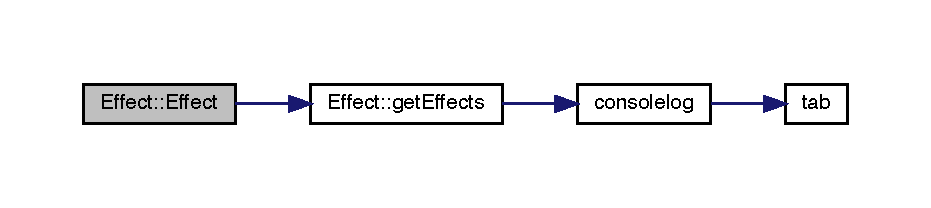
\includegraphics[width=350pt]{class_effect_a6ab7116f826b2607ada4630759f6afc5_cgraph}
\end{center}
\end{figure}
\mbox{\Hypertarget{class_effect_a2fbf9d2526c65543157370f68cbed091}\label{class_effect_a2fbf9d2526c65543157370f68cbed091}} 
\index{Effect@{Effect}!Effect@{Effect}}
\index{Effect@{Effect}!Effect@{Effect}}
\subsubsection{\texorpdfstring{Effect()}{Effect()}\hspace{0.1cm}{\footnotesize\ttfamily [2/2]}}
{\footnotesize\ttfamily Effect\+::\+Effect (\begin{DoxyParamCaption}\item[{\hyperlink{class_effect_a6422fe21e9e452943fbc3344884a6fed}{Effect\+::effect\+ID}}]{effect,  }\item[{std\+::map$<$ std\+::string, std\+::string $>$}]{params,  }\item[{int}]{fs }\end{DoxyParamCaption})}


\begin{DoxyParams}{Parameters}
{\em effect} & effect ID \\
\hline
{\em params} & map of effect parameters \\
\hline
{\em fs} & signal sampling frequency \\
\hline
\end{DoxyParams}


Definition at line 24 of file Effect.\+cpp.

Here is the call graph for this function\+:
\nopagebreak
\begin{figure}[H]
\begin{center}
\leavevmode
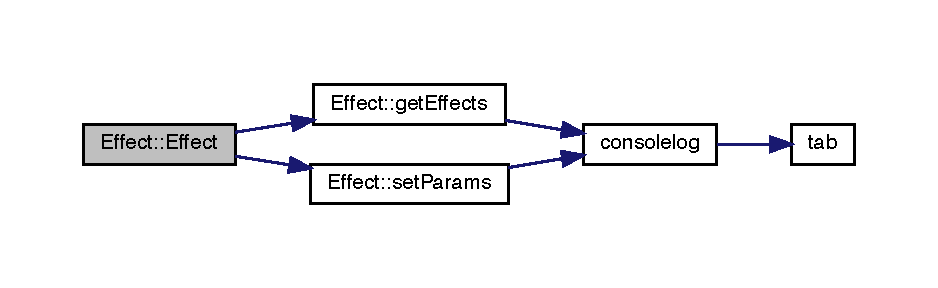
\includegraphics[width=350pt]{class_effect_a2fbf9d2526c65543157370f68cbed091_cgraph}
\end{center}
\end{figure}


\subsection{Member Function Documentation}
\mbox{\Hypertarget{class_effect_a6d212ada944f12afbcd8e3e6e623df51}\label{class_effect_a6d212ada944f12afbcd8e3e6e623df51}} 
\index{Effect@{Effect}!apply@{apply}}
\index{apply@{apply}!Effect@{Effect}}
\subsubsection{\texorpdfstring{apply()}{apply()}}
{\footnotesize\ttfamily bool Effect\+::apply (\begin{DoxyParamCaption}\item[{float $\ast$$\ast$}]{input,  }\item[{float $\ast$$\ast$}]{output,  }\item[{int}]{samples,  }\item[{std\+::vector$<$ \hyperlink{struct_s_a_c_bitstream_1_1_channel_type_a31c32b34085c06a1c58d920ca28c17c9}{S\+A\+C\+Bitstream\+::\+Channel\+Type\+::channeltype} $>$}]{channels }\end{DoxyParamCaption})}


\begin{DoxyParams}{Parameters}
{\em input} & input data pointer \\
\hline
{\em output} & output data pointer \\
\hline
{\em samples} & number of samples \\
\hline
{\em channels} & vector of channel types \\
\hline
\end{DoxyParams}
\begin{DoxyReturn}{Returns}
true if it was successful 
\end{DoxyReturn}


Definition at line 70 of file Effect.\+cpp.

Here is the call graph for this function\+:
\nopagebreak
\begin{figure}[H]
\begin{center}
\leavevmode
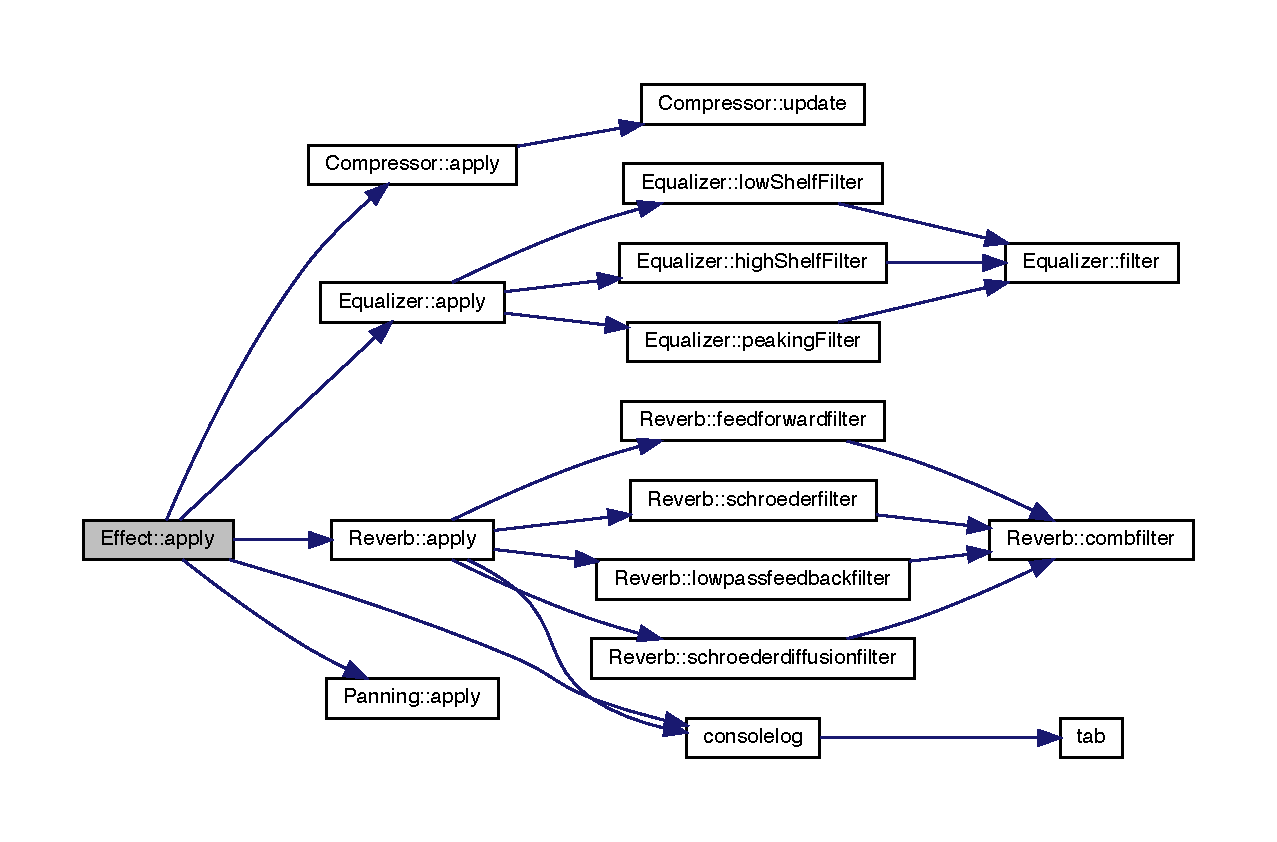
\includegraphics[width=350pt]{class_effect_a6d212ada944f12afbcd8e3e6e623df51_cgraph}
\end{center}
\end{figure}
Here is the caller graph for this function\+:
\nopagebreak
\begin{figure}[H]
\begin{center}
\leavevmode
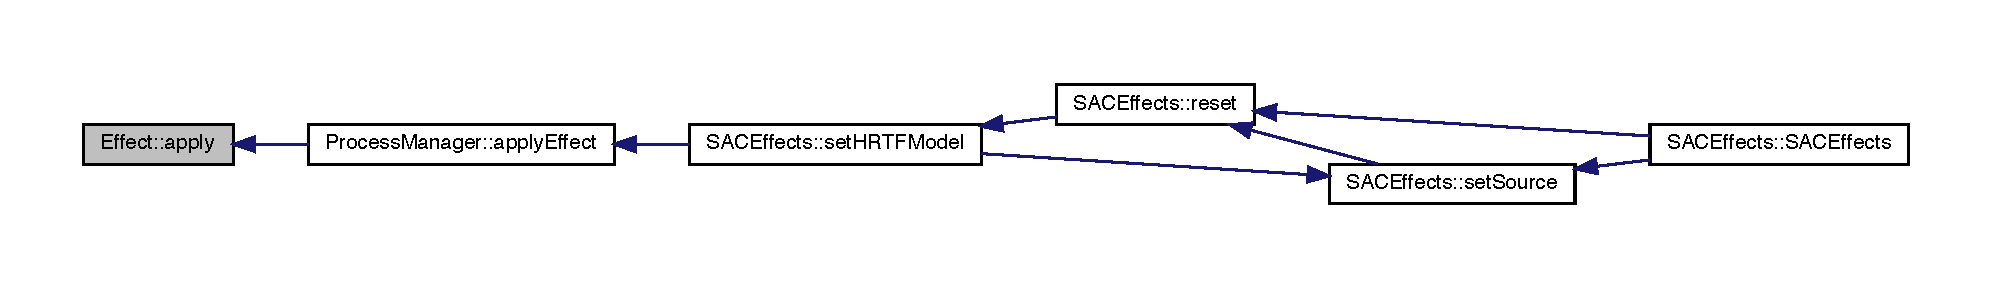
\includegraphics[width=350pt]{class_effect_a6d212ada944f12afbcd8e3e6e623df51_icgraph}
\end{center}
\end{figure}
\mbox{\Hypertarget{class_effect_ae108c1645f18162929cd5c272a30f74e}\label{class_effect_ae108c1645f18162929cd5c272a30f74e}} 
\index{Effect@{Effect}!get\+Channels@{get\+Channels}}
\index{get\+Channels@{get\+Channels}!Effect@{Effect}}
\subsubsection{\texorpdfstring{get\+Channels()}{getChannels()}}
{\footnotesize\ttfamily std\+::vector$<$ bool $>$ Effect\+::get\+Channels (\begin{DoxyParamCaption}\item[{std\+::string}]{configuration,  }\item[{int}]{size }\end{DoxyParamCaption})\hspace{0.3cm}{\ttfamily [static]}}


\begin{DoxyParams}{Parameters}
{\em configuration} & contained text of a effect configuration file (.fx) \\
\hline
{\em size} & number of channels \\
\hline
\end{DoxyParams}
\begin{DoxyReturn}{Returns}
channels boolean vector to select channels when applying effects 
\end{DoxyReturn}


Definition at line 162 of file Effect.\+cpp.

Here is the call graph for this function\+:
\nopagebreak
\begin{figure}[H]
\begin{center}
\leavevmode
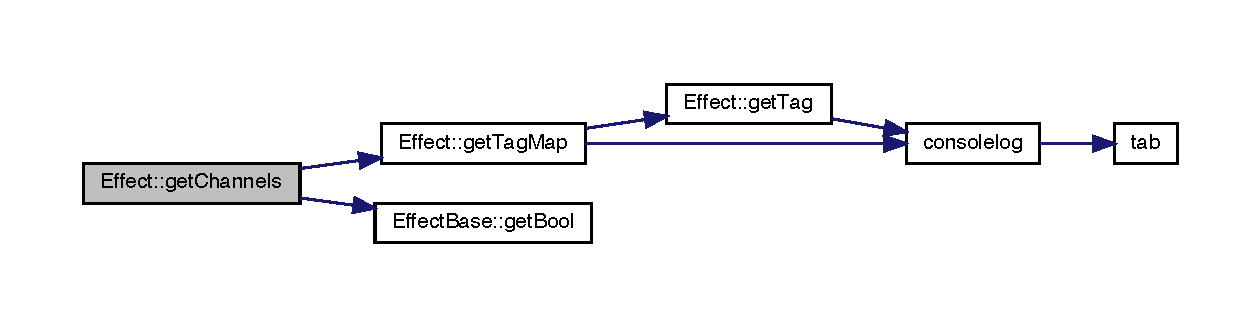
\includegraphics[width=350pt]{class_effect_ae108c1645f18162929cd5c272a30f74e_cgraph}
\end{center}
\end{figure}
\mbox{\Hypertarget{class_effect_a32185d446a9dc77963a322b64d2f9e27}\label{class_effect_a32185d446a9dc77963a322b64d2f9e27}} 
\index{Effect@{Effect}!get\+Effect@{get\+Effect}}
\index{get\+Effect@{get\+Effect}!Effect@{Effect}}
\subsubsection{\texorpdfstring{get\+Effect()}{getEffect()}}
{\footnotesize\ttfamily \hyperlink{class_effect_a6422fe21e9e452943fbc3344884a6fed}{Effect\+::effect\+ID} Effect\+::get\+Effect (\begin{DoxyParamCaption}\item[{std\+::string}]{effectname }\end{DoxyParamCaption})\hspace{0.3cm}{\ttfamily [static]}}


\begin{DoxyParams}{Parameters}
{\em effectname} & effect name string \\
\hline
\end{DoxyParams}
\begin{DoxyReturn}{Returns}
effect type \hyperlink{class_effect_a6422fe21e9e452943fbc3344884a6fed}{effect\+ID} 
\end{DoxyReturn}


Definition at line 141 of file Effect.\+cpp.

Here is the call graph for this function\+:
\nopagebreak
\begin{figure}[H]
\begin{center}
\leavevmode
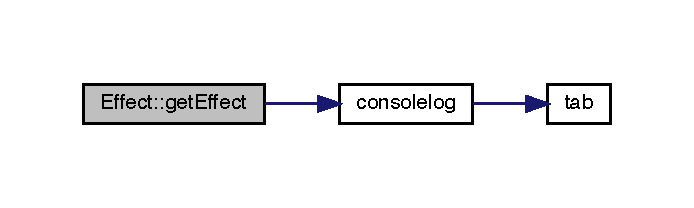
\includegraphics[width=333pt]{class_effect_a32185d446a9dc77963a322b64d2f9e27_cgraph}
\end{center}
\end{figure}
Here is the caller graph for this function\+:
\nopagebreak
\begin{figure}[H]
\begin{center}
\leavevmode
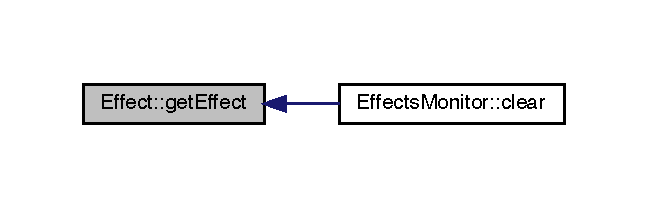
\includegraphics[width=311pt]{class_effect_a32185d446a9dc77963a322b64d2f9e27_icgraph}
\end{center}
\end{figure}
\mbox{\Hypertarget{class_effect_a2165f76956c91baf1482d2405eb1ed4e}\label{class_effect_a2165f76956c91baf1482d2405eb1ed4e}} 
\index{Effect@{Effect}!get\+Effects@{get\+Effects}}
\index{get\+Effects@{get\+Effects}!Effect@{Effect}}
\subsubsection{\texorpdfstring{get\+Effects()}{getEffects()}}
{\footnotesize\ttfamily std\+::map$<$ \hyperlink{class_effect_a6422fe21e9e452943fbc3344884a6fed}{Effect\+::effect\+ID}, std\+::string $>$ Effect\+::get\+Effects (\begin{DoxyParamCaption}{ }\end{DoxyParamCaption})\hspace{0.3cm}{\ttfamily [static]}}

\begin{DoxyReturn}{Returns}
map of available effects 
\end{DoxyReturn}


Definition at line 115 of file Effect.\+cpp.

Here is the call graph for this function\+:
\nopagebreak
\begin{figure}[H]
\begin{center}
\leavevmode
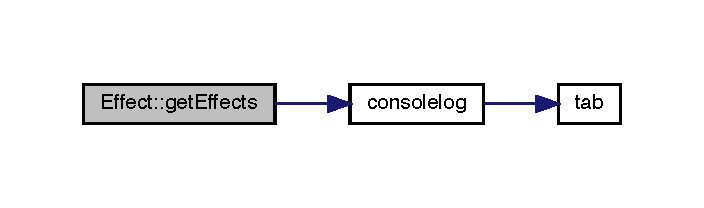
\includegraphics[width=338pt]{class_effect_a2165f76956c91baf1482d2405eb1ed4e_cgraph}
\end{center}
\end{figure}
Here is the caller graph for this function\+:
\nopagebreak
\begin{figure}[H]
\begin{center}
\leavevmode
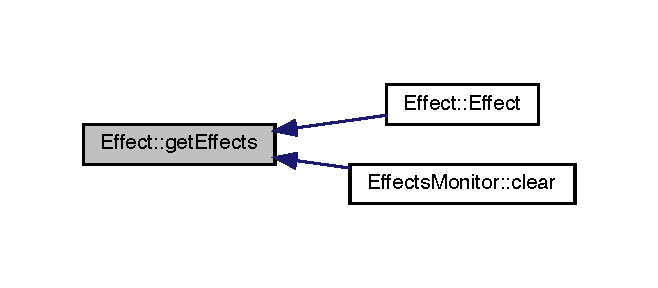
\includegraphics[width=316pt]{class_effect_a2165f76956c91baf1482d2405eb1ed4e_icgraph}
\end{center}
\end{figure}
\mbox{\Hypertarget{class_effect_ad0f19e11abff1f815c8b3b36b1f28c92}\label{class_effect_ad0f19e11abff1f815c8b3b36b1f28c92}} 
\index{Effect@{Effect}!get\+Levels@{get\+Levels}}
\index{get\+Levels@{get\+Levels}!Effect@{Effect}}
\subsubsection{\texorpdfstring{get\+Levels()}{getLevels()}}
{\footnotesize\ttfamily std\+::vector$<$ double $>$ Effect\+::get\+Levels (\begin{DoxyParamCaption}\item[{std\+::string}]{configuration,  }\item[{int}]{size }\end{DoxyParamCaption})\hspace{0.3cm}{\ttfamily [static]}}


\begin{DoxyParams}{Parameters}
{\em configuration} & contained text of a effect configuration file (.fx) \\
\hline
{\em size} & number of channels \\
\hline
\end{DoxyParams}
\begin{DoxyReturn}{Returns}
levels vector of input channels before applying effects 
\end{DoxyReturn}


Definition at line 178 of file Effect.\+cpp.

Here is the call graph for this function\+:
\nopagebreak
\begin{figure}[H]
\begin{center}
\leavevmode
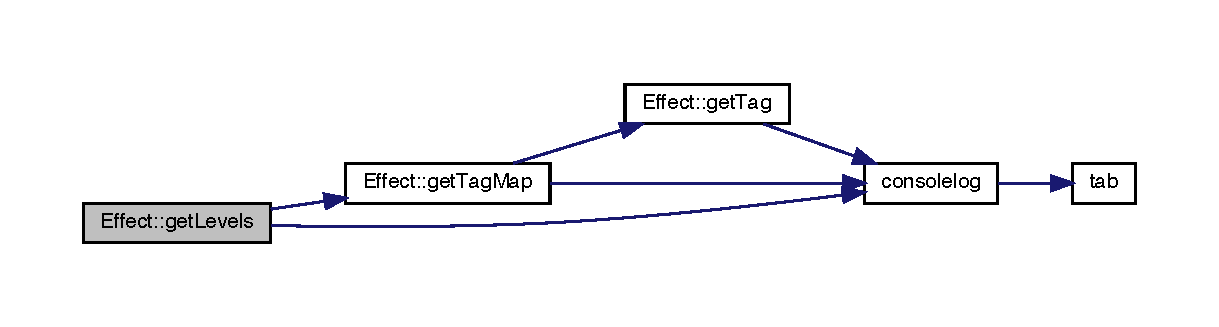
\includegraphics[width=350pt]{class_effect_ad0f19e11abff1f815c8b3b36b1f28c92_cgraph}
\end{center}
\end{figure}
\mbox{\Hypertarget{class_effect_ac322ae94a6b15b2d81053a55ce7542e2}\label{class_effect_ac322ae94a6b15b2d81053a55ce7542e2}} 
\index{Effect@{Effect}!get\+Params@{get\+Params}}
\index{get\+Params@{get\+Params}!Effect@{Effect}}
\subsubsection{\texorpdfstring{get\+Params()}{getParams()}}
{\footnotesize\ttfamily std\+::map$<$ std\+::string, std\+::string $>$ Effect\+::get\+Params (\begin{DoxyParamCaption}\item[{std\+::string}]{configuration }\end{DoxyParamCaption})\hspace{0.3cm}{\ttfamily [static]}}


\begin{DoxyParams}{Parameters}
{\em configuration} & contained text of a effect configuration file (.fx) \\
\hline
\end{DoxyParams}
\begin{DoxyReturn}{Returns}
parameters map variable valid to apply effects 
\end{DoxyReturn}


Definition at line 200 of file Effect.\+cpp.

Here is the call graph for this function\+:
\nopagebreak
\begin{figure}[H]
\begin{center}
\leavevmode
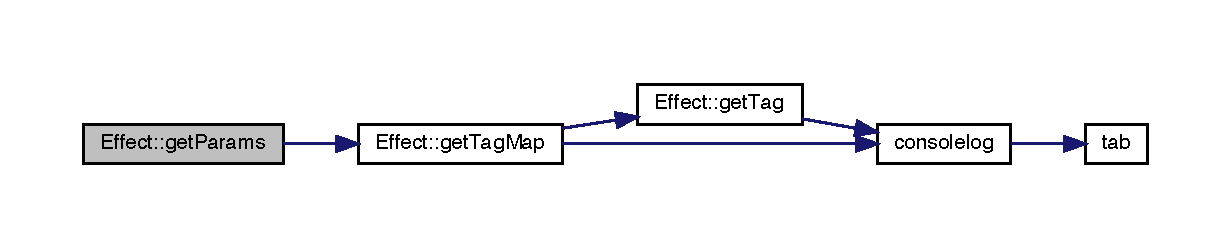
\includegraphics[width=350pt]{class_effect_ac322ae94a6b15b2d81053a55ce7542e2_cgraph}
\end{center}
\end{figure}
\mbox{\Hypertarget{class_effect_a607ab2a63d333137c1f07cf03611c4bf}\label{class_effect_a607ab2a63d333137c1f07cf03611c4bf}} 
\index{Effect@{Effect}!get\+Tag@{get\+Tag}}
\index{get\+Tag@{get\+Tag}!Effect@{Effect}}
\subsubsection{\texorpdfstring{get\+Tag()}{getTag()}}
{\footnotesize\ttfamily std\+::string Effect\+::get\+Tag (\begin{DoxyParamCaption}\item[{std\+::string}]{configuration,  }\item[{std\+::string}]{tag }\end{DoxyParamCaption})\hspace{0.3cm}{\ttfamily [static]}}


\begin{DoxyParams}{Parameters}
{\em configuration} & contained text of a effect configuration file (.fx) \\
\hline
{\em tag} & tag name of the requested field \\
\hline
\end{DoxyParams}
\begin{DoxyReturn}{Returns}
contained value in the tag 
\end{DoxyReturn}


Definition at line 211 of file Effect.\+cpp.

Here is the call graph for this function\+:
\nopagebreak
\begin{figure}[H]
\begin{center}
\leavevmode
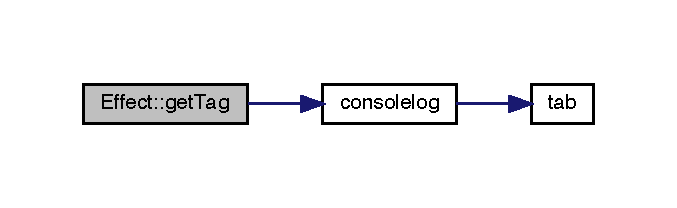
\includegraphics[width=325pt]{class_effect_a607ab2a63d333137c1f07cf03611c4bf_cgraph}
\end{center}
\end{figure}
Here is the caller graph for this function\+:
\nopagebreak
\begin{figure}[H]
\begin{center}
\leavevmode
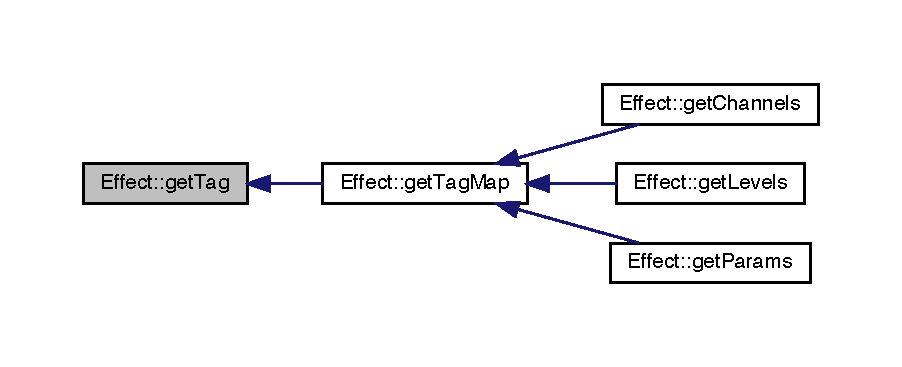
\includegraphics[width=350pt]{class_effect_a607ab2a63d333137c1f07cf03611c4bf_icgraph}
\end{center}
\end{figure}
\mbox{\Hypertarget{class_effect_a616281286b866f1f8f6c66715e54ee89}\label{class_effect_a616281286b866f1f8f6c66715e54ee89}} 
\index{Effect@{Effect}!get\+Tag\+Map@{get\+Tag\+Map}}
\index{get\+Tag\+Map@{get\+Tag\+Map}!Effect@{Effect}}
\subsubsection{\texorpdfstring{get\+Tag\+Map()}{getTagMap()}}
{\footnotesize\ttfamily std\+::map$<$ std\+::string, std\+::string $>$ Effect\+::get\+Tag\+Map (\begin{DoxyParamCaption}\item[{std\+::string}]{configuration,  }\item[{std\+::string}]{tag }\end{DoxyParamCaption})\hspace{0.3cm}{\ttfamily [static]}}


\begin{DoxyParams}{Parameters}
{\em configuration} & contained text of a effect configuration file (.fx) \\
\hline
{\em tag} & tag name of the requested field \\
\hline
\end{DoxyParams}
\begin{DoxyReturn}{Returns}
contained map of values in the tag 
\end{DoxyReturn}


Definition at line 224 of file Effect.\+cpp.

Here is the call graph for this function\+:
\nopagebreak
\begin{figure}[H]
\begin{center}
\leavevmode
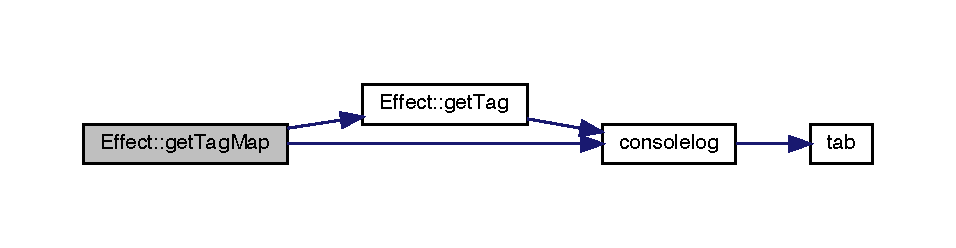
\includegraphics[width=350pt]{class_effect_a616281286b866f1f8f6c66715e54ee89_cgraph}
\end{center}
\end{figure}
Here is the caller graph for this function\+:
\nopagebreak
\begin{figure}[H]
\begin{center}
\leavevmode
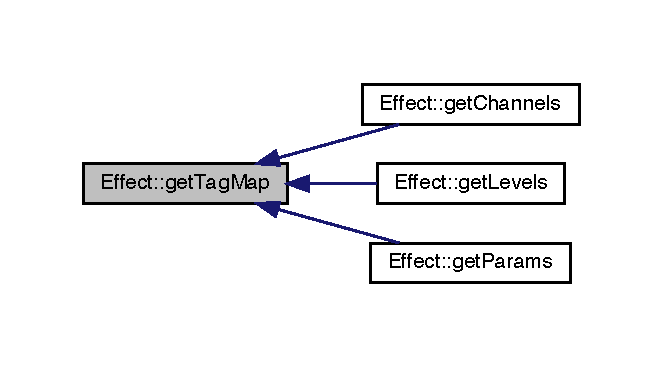
\includegraphics[width=318pt]{class_effect_a616281286b866f1f8f6c66715e54ee89_icgraph}
\end{center}
\end{figure}
\mbox{\Hypertarget{class_effect_ac2c35ce7382d627f20879b44be0e8132}\label{class_effect_ac2c35ce7382d627f20879b44be0e8132}} 
\index{Effect@{Effect}!plot@{plot}}
\index{plot@{plot}!Effect@{Effect}}
\subsubsection{\texorpdfstring{plot()}{plot()}}
{\footnotesize\ttfamily std\+::vector$<$ std\+::vector$<$ double $>$ $>$ Effect\+::plot (\begin{DoxyParamCaption}\item[{std\+::string}]{chart }\end{DoxyParamCaption})}


\begin{DoxyParams}{Parameters}
{\em chart} & chart id \\
\hline
\end{DoxyParams}
\begin{DoxyReturn}{Returns}
array of values as values\mbox{[}axis\mbox{]}\mbox{[}sample\mbox{]} axis\+: 0 = x (horizontal) and 1 = y (vertical) 
\end{DoxyReturn}


Definition at line 100 of file Effect.\+cpp.

Here is the call graph for this function\+:
\nopagebreak
\begin{figure}[H]
\begin{center}
\leavevmode
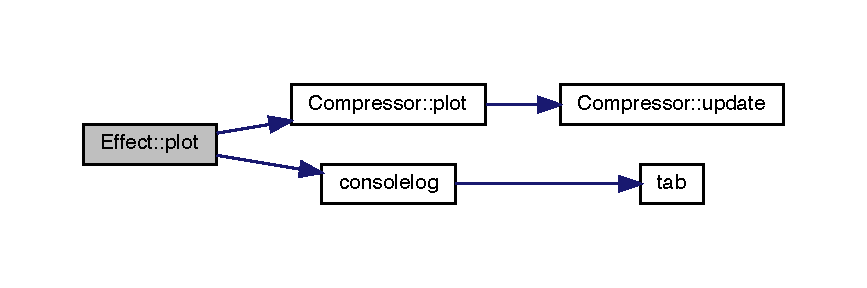
\includegraphics[width=350pt]{class_effect_ac2c35ce7382d627f20879b44be0e8132_cgraph}
\end{center}
\end{figure}
Here is the caller graph for this function\+:
\nopagebreak
\begin{figure}[H]
\begin{center}
\leavevmode
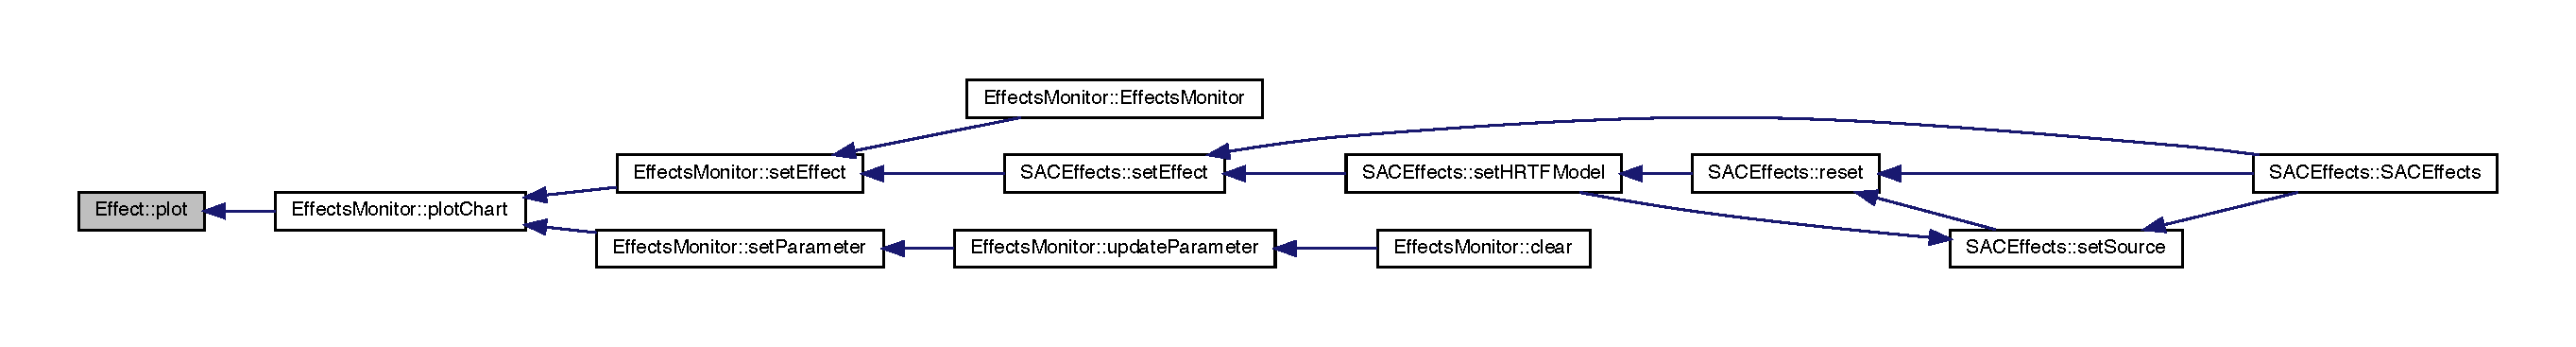
\includegraphics[width=350pt]{class_effect_ac2c35ce7382d627f20879b44be0e8132_icgraph}
\end{center}
\end{figure}
\mbox{\Hypertarget{class_effect_af0094495d423173463fd3e9cd40789af}\label{class_effect_af0094495d423173463fd3e9cd40789af}} 
\index{Effect@{Effect}!set\+Params@{set\+Params}}
\index{set\+Params@{set\+Params}!Effect@{Effect}}
\subsubsection{\texorpdfstring{set\+Params()}{setParams()}}
{\footnotesize\ttfamily void Effect\+::set\+Params (\begin{DoxyParamCaption}\item[{std\+::map$<$ std\+::string, std\+::string $>$}]{params }\end{DoxyParamCaption})}


\begin{DoxyParams}{Parameters}
{\em params} & parameters variable \\
\hline
\end{DoxyParams}


Definition at line 40 of file Effect.\+cpp.

Here is the call graph for this function\+:
\nopagebreak
\begin{figure}[H]
\begin{center}
\leavevmode
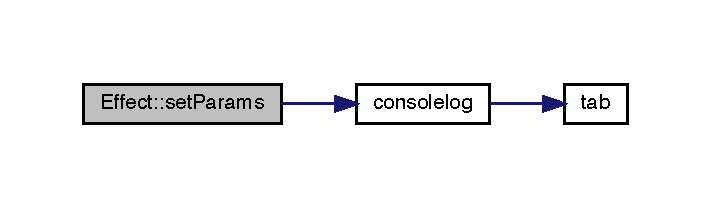
\includegraphics[width=341pt]{class_effect_af0094495d423173463fd3e9cd40789af_cgraph}
\end{center}
\end{figure}
Here is the caller graph for this function\+:
\nopagebreak
\begin{figure}[H]
\begin{center}
\leavevmode
\includegraphics[width=350pt]{class_effect_af0094495d423173463fd3e9cd40789af_icgraph}
\end{center}
\end{figure}


\subsection{Member Data Documentation}
\mbox{\Hypertarget{class_effect_ae23ae4e48c344fa374730a9ae24e7ad3}\label{class_effect_ae23ae4e48c344fa374730a9ae24e7ad3}} 
\index{Effect@{Effect}!effect@{effect}}
\index{effect@{effect}!Effect@{Effect}}
\subsubsection{\texorpdfstring{effect}{effect}}
{\footnotesize\ttfamily std\+::pair$<$\hyperlink{class_effect_a6422fe21e9e452943fbc3344884a6fed}{Effect\+::effect\+ID}, std\+::string$>$ Effect\+::effect}

selected effect name and id 

Definition at line 53 of file Effect.\+h.



The documentation for this class was generated from the following files\+:\begin{DoxyCompactItemize}
\item 
src/effects/Effect.\+h\item 
src/effects/Effect.\+cpp\end{DoxyCompactItemize}

\hypertarget{class_effect_base}{}\section{Effect\+Base Class Reference}
\label{class_effect_base}\index{Effect\+Base@{Effect\+Base}}


\hyperlink{class_effect}{Effect} base class.  




{\ttfamily \#include $<$Effect\+Base.\+h$>$}

\subsection*{Public Member Functions}
\begin{DoxyCompactItemize}
\item 
\mbox{\Hypertarget{class_effect_base_afcb5e7c5f5a689d7dc00d30eeefe5045}\label{class_effect_base_afcb5e7c5f5a689d7dc00d30eeefe5045}} 
\hyperlink{class_effect_base_afcb5e7c5f5a689d7dc00d30eeefe5045}{Effect\+Base} ()
\begin{DoxyCompactList}\small\item\em \hyperlink{class_effect_base}{Effect\+Base} constructor. \end{DoxyCompactList}\end{DoxyCompactItemize}
\subsection*{Static Public Member Functions}
\begin{DoxyCompactItemize}
\item 
static int \hyperlink{class_effect_base_aa2c8a7dfd4511cbb41f5ca1afd14cbb5}{get\+Int} (std\+::string param)
\begin{DoxyCompactList}\small\item\em It parses a parameter value to double. \end{DoxyCompactList}\item 
static double \hyperlink{class_effect_base_a29ac04c6135b4a202c0fab169f97f436}{get\+Double} (std\+::string param)
\begin{DoxyCompactList}\small\item\em It parses a parameter value to integer. \end{DoxyCompactList}\item 
static std\+::string \hyperlink{class_effect_base_a74b8d00a78daa5a33db20543564c7350}{get\+String} (std\+::string param)
\begin{DoxyCompactList}\small\item\em It parses a parameter value to string. \end{DoxyCompactList}\item 
static bool \hyperlink{class_effect_base_a5ce32d92ebf6973d177d0f8d1be8e8ba}{get\+Bool} (std\+::string param)
\begin{DoxyCompactList}\small\item\em It parses a parameter value to bool. \end{DoxyCompactList}\end{DoxyCompactItemize}
\subsection*{Static Public Attributes}
\begin{DoxyCompactItemize}
\item 
static int \hyperlink{class_effect_base_a18021994da076630edfe26d69fd1384f}{fs}
\item 
static std\+::map$<$ std\+::string, std\+::string $>$ \hyperlink{class_effect_base_a593c207eb855ae1bc37069766da29c9a}{params}
\end{DoxyCompactItemize}


\subsection{Detailed Description}
\begin{DoxyAuthor}{Author}
Andrés González Fornell 
\end{DoxyAuthor}


Definition at line 21 of file Effect\+Base.\+h.



\subsection{Member Function Documentation}
\mbox{\Hypertarget{class_effect_base_a5ce32d92ebf6973d177d0f8d1be8e8ba}\label{class_effect_base_a5ce32d92ebf6973d177d0f8d1be8e8ba}} 
\index{Effect\+Base@{Effect\+Base}!get\+Bool@{get\+Bool}}
\index{get\+Bool@{get\+Bool}!Effect\+Base@{Effect\+Base}}
\subsubsection{\texorpdfstring{get\+Bool()}{getBool()}}
{\footnotesize\ttfamily bool Effect\+Base\+::get\+Bool (\begin{DoxyParamCaption}\item[{std\+::string}]{param }\end{DoxyParamCaption})\hspace{0.3cm}{\ttfamily [static]}}


\begin{DoxyParams}{Parameters}
{\em param} & parameter value \\
\hline
\end{DoxyParams}
\begin{DoxyReturn}{Returns}
boolean value (false by default) 
\end{DoxyReturn}


Definition at line 314 of file Effect.\+cpp.

Here is the caller graph for this function\+:
\nopagebreak
\begin{figure}[H]
\begin{center}
\leavevmode
\includegraphics[width=324pt]{class_effect_base_a5ce32d92ebf6973d177d0f8d1be8e8ba_icgraph}
\end{center}
\end{figure}
\mbox{\Hypertarget{class_effect_base_a29ac04c6135b4a202c0fab169f97f436}\label{class_effect_base_a29ac04c6135b4a202c0fab169f97f436}} 
\index{Effect\+Base@{Effect\+Base}!get\+Double@{get\+Double}}
\index{get\+Double@{get\+Double}!Effect\+Base@{Effect\+Base}}
\subsubsection{\texorpdfstring{get\+Double()}{getDouble()}}
{\footnotesize\ttfamily double Effect\+Base\+::get\+Double (\begin{DoxyParamCaption}\item[{std\+::string}]{param }\end{DoxyParamCaption})\hspace{0.3cm}{\ttfamily [static]}}


\begin{DoxyParams}{Parameters}
{\em param} & parameter value \\
\hline
\end{DoxyParams}
\begin{DoxyReturn}{Returns}
value 
\end{DoxyReturn}


Definition at line 289 of file Effect.\+cpp.

\mbox{\Hypertarget{class_effect_base_aa2c8a7dfd4511cbb41f5ca1afd14cbb5}\label{class_effect_base_aa2c8a7dfd4511cbb41f5ca1afd14cbb5}} 
\index{Effect\+Base@{Effect\+Base}!get\+Int@{get\+Int}}
\index{get\+Int@{get\+Int}!Effect\+Base@{Effect\+Base}}
\subsubsection{\texorpdfstring{get\+Int()}{getInt()}}
{\footnotesize\ttfamily int Effect\+Base\+::get\+Int (\begin{DoxyParamCaption}\item[{std\+::string}]{param }\end{DoxyParamCaption})\hspace{0.3cm}{\ttfamily [static]}}


\begin{DoxyParams}{Parameters}
{\em param} & parameter value \\
\hline
\end{DoxyParams}
\begin{DoxyReturn}{Returns}
value as integer 
\end{DoxyReturn}


Definition at line 280 of file Effect.\+cpp.

\mbox{\Hypertarget{class_effect_base_a74b8d00a78daa5a33db20543564c7350}\label{class_effect_base_a74b8d00a78daa5a33db20543564c7350}} 
\index{Effect\+Base@{Effect\+Base}!get\+String@{get\+String}}
\index{get\+String@{get\+String}!Effect\+Base@{Effect\+Base}}
\subsubsection{\texorpdfstring{get\+String()}{getString()}}
{\footnotesize\ttfamily std\+::string Effect\+Base\+::get\+String (\begin{DoxyParamCaption}\item[{std\+::string}]{param }\end{DoxyParamCaption})\hspace{0.3cm}{\ttfamily [static]}}


\begin{DoxyParams}{Parameters}
{\em param} & parameter value \\
\hline
\end{DoxyParams}
\begin{DoxyReturn}{Returns}
value 
\end{DoxyReturn}


Definition at line 298 of file Effect.\+cpp.

Here is the call graph for this function\+:
\nopagebreak
\begin{figure}[H]
\begin{center}
\leavevmode
\includegraphics[width=350pt]{class_effect_base_a74b8d00a78daa5a33db20543564c7350_cgraph}
\end{center}
\end{figure}


\subsection{Member Data Documentation}
\mbox{\Hypertarget{class_effect_base_a18021994da076630edfe26d69fd1384f}\label{class_effect_base_a18021994da076630edfe26d69fd1384f}} 
\index{Effect\+Base@{Effect\+Base}!fs@{fs}}
\index{fs@{fs}!Effect\+Base@{Effect\+Base}}
\subsubsection{\texorpdfstring{fs}{fs}}
{\footnotesize\ttfamily int Effect\+Base\+::fs\hspace{0.3cm}{\ttfamily [static]}}

signal sampling frequency \mbox{[}Hz\mbox{]} 

Definition at line 23 of file Effect\+Base.\+h.

\mbox{\Hypertarget{class_effect_base_a593c207eb855ae1bc37069766da29c9a}\label{class_effect_base_a593c207eb855ae1bc37069766da29c9a}} 
\index{Effect\+Base@{Effect\+Base}!params@{params}}
\index{params@{params}!Effect\+Base@{Effect\+Base}}
\subsubsection{\texorpdfstring{params}{params}}
{\footnotesize\ttfamily std\+::map$<$ std\+::string, std\+::string $>$ Effect\+Base\+::params\hspace{0.3cm}{\ttfamily [static]}}

string of effect parameters 

Definition at line 24 of file Effect\+Base.\+h.



The documentation for this class was generated from the following files\+:\begin{DoxyCompactItemize}
\item 
src/effects/Effect\+Base.\+h\item 
src/effects/Effect.\+cpp\end{DoxyCompactItemize}

\hypertarget{class_effects_monitor}{}\section{Effects\+Monitor Class Reference}
\label{class_effects_monitor}\index{Effects\+Monitor@{Effects\+Monitor}}


Class for managing effects parameters.  




{\ttfamily \#include $<$Effects\+Monitor.\+h$>$}



Inheritance diagram for Effects\+Monitor\+:
\nopagebreak
\begin{figure}[H]
\begin{center}
\leavevmode
\includegraphics[width=160pt]{class_effects_monitor__inherit__graph}
\end{center}
\end{figure}


Collaboration diagram for Effects\+Monitor\+:
\nopagebreak
\begin{figure}[H]
\begin{center}
\leavevmode
\includegraphics[width=194pt]{class_effects_monitor__coll__graph}
\end{center}
\end{figure}
\subsection*{Public Slots}
\begin{Indent}\textbf{ Parameters slots}\par
{\em User interface functions for effect parameters control. }\begin{DoxyCompactItemize}
\item 
void \hyperlink{class_effects_monitor_ae2cc992b9bb457da2a0cdab854a414ea}{update\+Parameter} (int value)
\begin{DoxyCompactList}\small\item\em Slot for updating parameters parameters of type int when one of them is changed. \end{DoxyCompactList}\item 
void \hyperlink{class_effects_monitor_aa32c90185185305770ad5ab911641e17}{update\+Parameter} (double value)
\begin{DoxyCompactList}\small\item\em Slot for updating parameters parameters of type double when one of them is changed. \end{DoxyCompactList}\item 
void \hyperlink{class_effects_monitor_ab2be23fba9628432cacdfc83cc75e9f4}{update\+Parameter} (Q\+String value)
\begin{DoxyCompactList}\small\item\em Slot for updating parameters of type string when one of them is changed. \end{DoxyCompactList}\item 
void \hyperlink{class_effects_monitor_a3488d6ae49a81de79fe6913a7bebcafe}{update\+Parameter} (bool value)
\begin{DoxyCompactList}\small\item\em Slot for updating parameters parameters of type bool and enum when one of them is changed. \end{DoxyCompactList}\end{DoxyCompactItemize}
\end{Indent}
\subsection*{Public Member Functions}
\begin{DoxyCompactItemize}
\item 
\hyperlink{class_effects_monitor_a484d2e47c270b1a9f608dd7c2c7e3994}{Effects\+Monitor} (Q\+Widget $\ast$framework)
\begin{DoxyCompactList}\small\item\em \hyperlink{class_effects_monitor}{Effects\+Monitor} constructor. \end{DoxyCompactList}\item 
\hyperlink{class_effects_monitor_ad9215233b6d88585ec5d31ca4f35771a}{Effects\+Monitor} (Q\+Widget $\ast$framework, \hyperlink{class_effect}{Effect} $\ast$\hyperlink{class_effects_monitor_a4ec98ceedd0d8bea006da1fc97f02124}{effect})
\begin{DoxyCompactList}\small\item\em \hyperlink{class_effects_monitor}{Effects\+Monitor} constructor. \end{DoxyCompactList}\item 
\mbox{\Hypertarget{class_effects_monitor_aeb3a098669694d424d02c3ed8294d923}\label{class_effects_monitor_aeb3a098669694d424d02c3ed8294d923}} 
\hyperlink{class_effects_monitor_aeb3a098669694d424d02c3ed8294d923}{$\sim$\+Effects\+Monitor} ()
\begin{DoxyCompactList}\small\item\em \hyperlink{class_effects_monitor}{Effects\+Monitor} destructor. \end{DoxyCompactList}\item 
void \hyperlink{class_effects_monitor_ade184df36063a2c7ef2855c12265bd78}{set\+Effect} (\hyperlink{class_effect}{Effect} $\ast$\hyperlink{class_effects_monitor_a4ec98ceedd0d8bea006da1fc97f02124}{effect})
\begin{DoxyCompactList}\small\item\em It selects an effect. \end{DoxyCompactList}\item 
\mbox{\Hypertarget{class_effects_monitor_ad6ad01ab2de7ca57a57e5fb71c2f85d9}\label{class_effects_monitor_ad6ad01ab2de7ca57a57e5fb71c2f85d9}} 
void \hyperlink{class_effects_monitor_ad6ad01ab2de7ca57a57e5fb71c2f85d9}{clear} ()
\begin{DoxyCompactList}\small\item\em It clears the user interface framework. \end{DoxyCompactList}\item 
void \hyperlink{class_effects_monitor_a96ff58c6076dd68e03aea26896b69d78}{set\+Parameter} (std\+::string key, std\+::string value)
\begin{DoxyCompactList}\small\item\em It sets a parameter from the parameter user interface object. \end{DoxyCompactList}\item 
\mbox{\Hypertarget{class_effects_monitor_a50df1e2902fde1839b541b3429f8f02d}\label{class_effects_monitor_a50df1e2902fde1839b541b3429f8f02d}} 
void \hyperlink{class_effects_monitor_a50df1e2902fde1839b541b3429f8f02d}{plot\+Chart} ()
\begin{DoxyCompactList}\small\item\em It plots every chart on the effects monitor. \end{DoxyCompactList}\end{DoxyCompactItemize}
\subsection*{Public Attributes}
\begin{DoxyCompactItemize}
\item 
\hyperlink{class_effect}{Effect} $\ast$ \hyperlink{class_effects_monitor_a4ec98ceedd0d8bea006da1fc97f02124}{effect}
\item 
std\+::map$<$ \hyperlink{class_effect_a6422fe21e9e452943fbc3344884a6fed}{Effect\+::effect\+ID}, std\+::string $>$ \hyperlink{class_effects_monitor_abf43aed9b7bcc0dee032f5e2e6a3e438}{effects}
\item 
std\+::map$<$ \hyperlink{class_effect_a6422fe21e9e452943fbc3344884a6fed}{Effect\+::effect\+ID}, std\+::string $>$ \hyperlink{class_effects_monitor_a88dbd80c419f86e09919761011c2a152}{files}
\item 
std\+::map$<$ std\+::string, std\+::string $>$ \hyperlink{class_effects_monitor_aae2cb43d0ee0c182eca7309c561071ba}{parameters}
\item 
std\+::map$<$ std\+::string, \hyperlink{class_chart2_d}{Chart2D} $\ast$ $>$ \hyperlink{class_effects_monitor_a2b5f5373404adac3f94bdab2f423d958}{charts}
\end{DoxyCompactItemize}


\subsection{Detailed Description}
\begin{DoxyAuthor}{Author}
Andrés González Fornell 
\end{DoxyAuthor}


Definition at line 33 of file Effects\+Monitor.\+h.



\subsection{Constructor \& Destructor Documentation}
\mbox{\Hypertarget{class_effects_monitor_a484d2e47c270b1a9f608dd7c2c7e3994}\label{class_effects_monitor_a484d2e47c270b1a9f608dd7c2c7e3994}} 
\index{Effects\+Monitor@{Effects\+Monitor}!Effects\+Monitor@{Effects\+Monitor}}
\index{Effects\+Monitor@{Effects\+Monitor}!Effects\+Monitor@{Effects\+Monitor}}
\subsubsection{\texorpdfstring{Effects\+Monitor()}{EffectsMonitor()}\hspace{0.1cm}{\footnotesize\ttfamily [1/2]}}
{\footnotesize\ttfamily Effects\+Monitor\+::\+Effects\+Monitor (\begin{DoxyParamCaption}\item[{Q\+Widget $\ast$}]{framework }\end{DoxyParamCaption})}


\begin{DoxyParams}{Parameters}
{\em framework} & user interface framework \\
\hline
\end{DoxyParams}


Definition at line 10 of file Effects\+Monitor.\+cpp.

Here is the call graph for this function\+:
\nopagebreak
\begin{figure}[H]
\begin{center}
\leavevmode
\includegraphics[width=350pt]{class_effects_monitor_a484d2e47c270b1a9f608dd7c2c7e3994_cgraph}
\end{center}
\end{figure}
\mbox{\Hypertarget{class_effects_monitor_ad9215233b6d88585ec5d31ca4f35771a}\label{class_effects_monitor_ad9215233b6d88585ec5d31ca4f35771a}} 
\index{Effects\+Monitor@{Effects\+Monitor}!Effects\+Monitor@{Effects\+Monitor}}
\index{Effects\+Monitor@{Effects\+Monitor}!Effects\+Monitor@{Effects\+Monitor}}
\subsubsection{\texorpdfstring{Effects\+Monitor()}{EffectsMonitor()}\hspace{0.1cm}{\footnotesize\ttfamily [2/2]}}
{\footnotesize\ttfamily Effects\+Monitor\+::\+Effects\+Monitor (\begin{DoxyParamCaption}\item[{Q\+Widget $\ast$}]{framework,  }\item[{\hyperlink{class_effect}{Effect} $\ast$}]{effect }\end{DoxyParamCaption})}


\begin{DoxyParams}{Parameters}
{\em framework} & user interface framework \\
\hline
{\em effect} & selected effect to be load \\
\hline
\end{DoxyParams}


Definition at line 23 of file Effects\+Monitor.\+cpp.

Here is the call graph for this function\+:
\nopagebreak
\begin{figure}[H]
\begin{center}
\leavevmode
\includegraphics[width=350pt]{class_effects_monitor_ad9215233b6d88585ec5d31ca4f35771a_cgraph}
\end{center}
\end{figure}


\subsection{Member Function Documentation}
\mbox{\Hypertarget{class_effects_monitor_ade184df36063a2c7ef2855c12265bd78}\label{class_effects_monitor_ade184df36063a2c7ef2855c12265bd78}} 
\index{Effects\+Monitor@{Effects\+Monitor}!set\+Effect@{set\+Effect}}
\index{set\+Effect@{set\+Effect}!Effects\+Monitor@{Effects\+Monitor}}
\subsubsection{\texorpdfstring{set\+Effect()}{setEffect()}}
{\footnotesize\ttfamily void Effects\+Monitor\+::set\+Effect (\begin{DoxyParamCaption}\item[{\hyperlink{class_effect}{Effect} $\ast$}]{effect }\end{DoxyParamCaption})}


\begin{DoxyParams}{Parameters}
{\em effect} & selected effect \\
\hline
\end{DoxyParams}


Definition at line 40 of file Effects\+Monitor.\+cpp.

Here is the call graph for this function\+:
\nopagebreak
\begin{figure}[H]
\begin{center}
\leavevmode
\includegraphics[width=350pt]{class_effects_monitor_ade184df36063a2c7ef2855c12265bd78_cgraph}
\end{center}
\end{figure}
Here is the caller graph for this function\+:
\nopagebreak
\begin{figure}[H]
\begin{center}
\leavevmode
\includegraphics[width=350pt]{class_effects_monitor_ade184df36063a2c7ef2855c12265bd78_icgraph}
\end{center}
\end{figure}
\mbox{\Hypertarget{class_effects_monitor_a96ff58c6076dd68e03aea26896b69d78}\label{class_effects_monitor_a96ff58c6076dd68e03aea26896b69d78}} 
\index{Effects\+Monitor@{Effects\+Monitor}!set\+Parameter@{set\+Parameter}}
\index{set\+Parameter@{set\+Parameter}!Effects\+Monitor@{Effects\+Monitor}}
\subsubsection{\texorpdfstring{set\+Parameter()}{setParameter()}}
{\footnotesize\ttfamily void Effects\+Monitor\+::set\+Parameter (\begin{DoxyParamCaption}\item[{std\+::string}]{parameter,  }\item[{std\+::string}]{value }\end{DoxyParamCaption})}


\begin{DoxyParams}{Parameters}
{\em parameter} & parameter name \\
\hline
{\em value} & new parameter value \\
\hline
\end{DoxyParams}


Definition at line 362 of file Effects\+Monitor.\+cpp.

Here is the call graph for this function\+:
\nopagebreak
\begin{figure}[H]
\begin{center}
\leavevmode
\includegraphics[width=350pt]{class_effects_monitor_a96ff58c6076dd68e03aea26896b69d78_cgraph}
\end{center}
\end{figure}
Here is the caller graph for this function\+:
\nopagebreak
\begin{figure}[H]
\begin{center}
\leavevmode
\includegraphics[width=350pt]{class_effects_monitor_a96ff58c6076dd68e03aea26896b69d78_icgraph}
\end{center}
\end{figure}
\mbox{\Hypertarget{class_effects_monitor_ae2cc992b9bb457da2a0cdab854a414ea}\label{class_effects_monitor_ae2cc992b9bb457da2a0cdab854a414ea}} 
\index{Effects\+Monitor@{Effects\+Monitor}!update\+Parameter@{update\+Parameter}}
\index{update\+Parameter@{update\+Parameter}!Effects\+Monitor@{Effects\+Monitor}}
\subsubsection{\texorpdfstring{update\+Parameter}{updateParameter}\hspace{0.1cm}{\footnotesize\ttfamily [1/4]}}
{\footnotesize\ttfamily void Effects\+Monitor\+::update\+Parameter (\begin{DoxyParamCaption}\item[{int}]{value }\end{DoxyParamCaption})\hspace{0.3cm}{\ttfamily [slot]}}


\begin{DoxyParams}{Parameters}
{\em value} & changed value \\
\hline
\end{DoxyParams}


Definition at line 403 of file Effects\+Monitor.\+cpp.

Here is the call graph for this function\+:
\nopagebreak
\begin{figure}[H]
\begin{center}
\leavevmode
\includegraphics[width=350pt]{class_effects_monitor_ae2cc992b9bb457da2a0cdab854a414ea_cgraph}
\end{center}
\end{figure}
Here is the caller graph for this function\+:
\nopagebreak
\begin{figure}[H]
\begin{center}
\leavevmode
\includegraphics[width=350pt]{class_effects_monitor_ae2cc992b9bb457da2a0cdab854a414ea_icgraph}
\end{center}
\end{figure}
\mbox{\Hypertarget{class_effects_monitor_aa32c90185185305770ad5ab911641e17}\label{class_effects_monitor_aa32c90185185305770ad5ab911641e17}} 
\index{Effects\+Monitor@{Effects\+Monitor}!update\+Parameter@{update\+Parameter}}
\index{update\+Parameter@{update\+Parameter}!Effects\+Monitor@{Effects\+Monitor}}
\subsubsection{\texorpdfstring{update\+Parameter}{updateParameter}\hspace{0.1cm}{\footnotesize\ttfamily [2/4]}}
{\footnotesize\ttfamily void Effects\+Monitor\+::update\+Parameter (\begin{DoxyParamCaption}\item[{double}]{value }\end{DoxyParamCaption})\hspace{0.3cm}{\ttfamily [slot]}}


\begin{DoxyParams}{Parameters}
{\em value} & changed value \\
\hline
\end{DoxyParams}


Definition at line 413 of file Effects\+Monitor.\+cpp.

Here is the call graph for this function\+:
\nopagebreak
\begin{figure}[H]
\begin{center}
\leavevmode
\includegraphics[width=350pt]{class_effects_monitor_aa32c90185185305770ad5ab911641e17_cgraph}
\end{center}
\end{figure}
\mbox{\Hypertarget{class_effects_monitor_ab2be23fba9628432cacdfc83cc75e9f4}\label{class_effects_monitor_ab2be23fba9628432cacdfc83cc75e9f4}} 
\index{Effects\+Monitor@{Effects\+Monitor}!update\+Parameter@{update\+Parameter}}
\index{update\+Parameter@{update\+Parameter}!Effects\+Monitor@{Effects\+Monitor}}
\subsubsection{\texorpdfstring{update\+Parameter}{updateParameter}\hspace{0.1cm}{\footnotesize\ttfamily [3/4]}}
{\footnotesize\ttfamily void Effects\+Monitor\+::update\+Parameter (\begin{DoxyParamCaption}\item[{Q\+String}]{value }\end{DoxyParamCaption})\hspace{0.3cm}{\ttfamily [slot]}}


\begin{DoxyParams}{Parameters}
{\em value} & changed value \\
\hline
\end{DoxyParams}


Definition at line 423 of file Effects\+Monitor.\+cpp.

Here is the call graph for this function\+:
\nopagebreak
\begin{figure}[H]
\begin{center}
\leavevmode
\includegraphics[width=350pt]{class_effects_monitor_ab2be23fba9628432cacdfc83cc75e9f4_cgraph}
\end{center}
\end{figure}
\mbox{\Hypertarget{class_effects_monitor_a3488d6ae49a81de79fe6913a7bebcafe}\label{class_effects_monitor_a3488d6ae49a81de79fe6913a7bebcafe}} 
\index{Effects\+Monitor@{Effects\+Monitor}!update\+Parameter@{update\+Parameter}}
\index{update\+Parameter@{update\+Parameter}!Effects\+Monitor@{Effects\+Monitor}}
\subsubsection{\texorpdfstring{update\+Parameter}{updateParameter}\hspace{0.1cm}{\footnotesize\ttfamily [4/4]}}
{\footnotesize\ttfamily void Effects\+Monitor\+::update\+Parameter (\begin{DoxyParamCaption}\item[{bool}]{value }\end{DoxyParamCaption})\hspace{0.3cm}{\ttfamily [slot]}}


\begin{DoxyParams}{Parameters}
{\em value} & changed value \\
\hline
\end{DoxyParams}


Definition at line 433 of file Effects\+Monitor.\+cpp.

Here is the call graph for this function\+:
\nopagebreak
\begin{figure}[H]
\begin{center}
\leavevmode
\includegraphics[width=350pt]{class_effects_monitor_a3488d6ae49a81de79fe6913a7bebcafe_cgraph}
\end{center}
\end{figure}


\subsection{Member Data Documentation}
\mbox{\Hypertarget{class_effects_monitor_a2b5f5373404adac3f94bdab2f423d958}\label{class_effects_monitor_a2b5f5373404adac3f94bdab2f423d958}} 
\index{Effects\+Monitor@{Effects\+Monitor}!charts@{charts}}
\index{charts@{charts}!Effects\+Monitor@{Effects\+Monitor}}
\subsubsection{\texorpdfstring{charts}{charts}}
{\footnotesize\ttfamily std\+::map$<$std\+::string, \hyperlink{class_chart2_d}{Chart2D} $\ast$$>$ Effects\+Monitor\+::charts}

list of charts of effect monitoring 

Definition at line 40 of file Effects\+Monitor.\+h.

\mbox{\Hypertarget{class_effects_monitor_a4ec98ceedd0d8bea006da1fc97f02124}\label{class_effects_monitor_a4ec98ceedd0d8bea006da1fc97f02124}} 
\index{Effects\+Monitor@{Effects\+Monitor}!effect@{effect}}
\index{effect@{effect}!Effects\+Monitor@{Effects\+Monitor}}
\subsubsection{\texorpdfstring{effect}{effect}}
{\footnotesize\ttfamily \hyperlink{class_effect}{Effect}$\ast$ Effects\+Monitor\+::effect}

pointer to current selected effect 

Definition at line 36 of file Effects\+Monitor.\+h.

\mbox{\Hypertarget{class_effects_monitor_abf43aed9b7bcc0dee032f5e2e6a3e438}\label{class_effects_monitor_abf43aed9b7bcc0dee032f5e2e6a3e438}} 
\index{Effects\+Monitor@{Effects\+Monitor}!effects@{effects}}
\index{effects@{effects}!Effects\+Monitor@{Effects\+Monitor}}
\subsubsection{\texorpdfstring{effects}{effects}}
{\footnotesize\ttfamily std\+::map$<$\hyperlink{class_effect_a6422fe21e9e452943fbc3344884a6fed}{Effect\+::effect\+ID}, std\+::string$>$ Effects\+Monitor\+::effects}

list of all available effects 

Definition at line 37 of file Effects\+Monitor.\+h.

\mbox{\Hypertarget{class_effects_monitor_a88dbd80c419f86e09919761011c2a152}\label{class_effects_monitor_a88dbd80c419f86e09919761011c2a152}} 
\index{Effects\+Monitor@{Effects\+Monitor}!files@{files}}
\index{files@{files}!Effects\+Monitor@{Effects\+Monitor}}
\subsubsection{\texorpdfstring{files}{files}}
{\footnotesize\ttfamily std\+::map$<$\hyperlink{class_effect_a6422fe21e9e452943fbc3344884a6fed}{Effect\+::effect\+ID}, std\+::string$>$ Effects\+Monitor\+::files}

list of all available effects template files 

Definition at line 38 of file Effects\+Monitor.\+h.

\mbox{\Hypertarget{class_effects_monitor_aae2cb43d0ee0c182eca7309c561071ba}\label{class_effects_monitor_aae2cb43d0ee0c182eca7309c561071ba}} 
\index{Effects\+Monitor@{Effects\+Monitor}!parameters@{parameters}}
\index{parameters@{parameters}!Effects\+Monitor@{Effects\+Monitor}}
\subsubsection{\texorpdfstring{parameters}{parameters}}
{\footnotesize\ttfamily std\+::map$<$std\+::string, std\+::string$>$ Effects\+Monitor\+::parameters}

list of the current effect parameters and their values 

Definition at line 39 of file Effects\+Monitor.\+h.



The documentation for this class was generated from the following files\+:\begin{DoxyCompactItemize}
\item 
src/interface/Effects\+Monitor.\+h\item 
src/interface/Effects\+Monitor.\+cpp\end{DoxyCompactItemize}

\hypertarget{class_encoder}{}\section{Encoder Class Reference}
\label{class_encoder}\index{Encoder@{Encoder}}


\hyperlink{class_encoder}{Encoder} window interface.  




{\ttfamily \#include $<$Encoder.\+h$>$}



Inheritance diagram for Encoder\+:
\nopagebreak
\begin{figure}[H]
\begin{center}
\leavevmode
\includegraphics[width=134pt]{class_encoder__inherit__graph}
\end{center}
\end{figure}


Collaboration diagram for Encoder\+:
\nopagebreak
\begin{figure}[H]
\begin{center}
\leavevmode
\includegraphics[width=307pt]{class_encoder__coll__graph}
\end{center}
\end{figure}
\subsection*{Public Member Functions}
\begin{DoxyCompactItemize}
\item 
\mbox{\Hypertarget{class_encoder_a0b084c3a7e670faafd9d651d6913d105}\label{class_encoder_a0b084c3a7e670faafd9d651d6913d105}} 
\hyperlink{class_encoder_a0b084c3a7e670faafd9d651d6913d105}{Encoder} (Q\+Widget $\ast$parent=0)
\begin{DoxyCompactList}\small\item\em \hyperlink{class_encoder}{Encoder} constructor. \end{DoxyCompactList}\item 
\mbox{\Hypertarget{class_encoder_a87cc8067c98c0ab2134dee3822e3b250}\label{class_encoder_a87cc8067c98c0ab2134dee3822e3b250}} 
\hyperlink{class_encoder_a87cc8067c98c0ab2134dee3822e3b250}{$\sim$\+Encoder} ()
\begin{DoxyCompactList}\small\item\em \hyperlink{class_encoder}{Encoder} destructor. \end{DoxyCompactList}\item 
void \hyperlink{class_encoder_af5623d0bd5fc7b1b2be27375d2994eb1}{set\+Input} (std\+::string filename)
\begin{DoxyCompactList}\small\item\em It sets the input audio file. \end{DoxyCompactList}\item 
void \hyperlink{class_encoder_a81e43409dc83e9118472a81ba65e6779}{set\+Output} (std\+::string filename)
\begin{DoxyCompactList}\small\item\em It sets the output audio file. \end{DoxyCompactList}\item 
void \hyperlink{class_encoder_adc879a1000d99660b36d7369e00f4f06}{set\+Tree} (int tree)
\begin{DoxyCompactList}\small\item\em It sets a tree configuration. \end{DoxyCompactList}\end{DoxyCompactItemize}
\subsection*{Public Attributes}
\begin{DoxyCompactItemize}
\item 
int \hyperlink{class_encoder_aa0549b597ab8fda7191f2e659a56044b}{fs}
\item 
\hyperlink{class_w_a_v_file}{W\+A\+V\+File} $\ast$ \hyperlink{class_encoder_aa851a11113fd12d5cfa04a4a72013157}{input}
\item 
\hyperlink{class_w_a_v_file}{W\+A\+V\+File} $\ast$ \hyperlink{class_encoder_ac4d4774d75750c1fdddd3740b7f30985}{output}
\item 
\hyperlink{class_file}{File} $\ast$ \hyperlink{class_encoder_a8cd18343fe80007dba58b4d716227544}{bitstream}
\end{DoxyCompactItemize}


\subsection{Detailed Description}
\begin{DoxyAuthor}{Author}
Andrés González Fornell 
\end{DoxyAuthor}


Definition at line 29 of file Encoder.\+h.



\subsection{Member Function Documentation}
\mbox{\Hypertarget{class_encoder_af5623d0bd5fc7b1b2be27375d2994eb1}\label{class_encoder_af5623d0bd5fc7b1b2be27375d2994eb1}} 
\index{Encoder@{Encoder}!set\+Input@{set\+Input}}
\index{set\+Input@{set\+Input}!Encoder@{Encoder}}
\subsubsection{\texorpdfstring{set\+Input()}{setInput()}}
{\footnotesize\ttfamily void Encoder\+::set\+Input (\begin{DoxyParamCaption}\item[{std\+::string}]{filename }\end{DoxyParamCaption})}


\begin{DoxyParams}{Parameters}
{\em filename} & file path \\
\hline
\end{DoxyParams}


Definition at line 52 of file Encoder.\+cpp.

Here is the call graph for this function\+:
\nopagebreak
\begin{figure}[H]
\begin{center}
\leavevmode
\includegraphics[width=350pt]{class_encoder_af5623d0bd5fc7b1b2be27375d2994eb1_cgraph}
\end{center}
\end{figure}
Here is the caller graph for this function\+:
\nopagebreak
\begin{figure}[H]
\begin{center}
\leavevmode
\includegraphics[width=308pt]{class_encoder_af5623d0bd5fc7b1b2be27375d2994eb1_icgraph}
\end{center}
\end{figure}
\mbox{\Hypertarget{class_encoder_a81e43409dc83e9118472a81ba65e6779}\label{class_encoder_a81e43409dc83e9118472a81ba65e6779}} 
\index{Encoder@{Encoder}!set\+Output@{set\+Output}}
\index{set\+Output@{set\+Output}!Encoder@{Encoder}}
\subsubsection{\texorpdfstring{set\+Output()}{setOutput()}}
{\footnotesize\ttfamily void Encoder\+::set\+Output (\begin{DoxyParamCaption}\item[{std\+::string}]{filename }\end{DoxyParamCaption})}


\begin{DoxyParams}{Parameters}
{\em filename} & file path \\
\hline
\end{DoxyParams}


Definition at line 85 of file Encoder.\+cpp.

Here is the call graph for this function\+:
\nopagebreak
\begin{figure}[H]
\begin{center}
\leavevmode
\includegraphics[width=350pt]{class_encoder_a81e43409dc83e9118472a81ba65e6779_cgraph}
\end{center}
\end{figure}
Here is the caller graph for this function\+:
\nopagebreak
\begin{figure}[H]
\begin{center}
\leavevmode
\includegraphics[width=312pt]{class_encoder_a81e43409dc83e9118472a81ba65e6779_icgraph}
\end{center}
\end{figure}
\mbox{\Hypertarget{class_encoder_adc879a1000d99660b36d7369e00f4f06}\label{class_encoder_adc879a1000d99660b36d7369e00f4f06}} 
\index{Encoder@{Encoder}!set\+Tree@{set\+Tree}}
\index{set\+Tree@{set\+Tree}!Encoder@{Encoder}}
\subsubsection{\texorpdfstring{set\+Tree()}{setTree()}}
{\footnotesize\ttfamily void Encoder\+::set\+Tree (\begin{DoxyParamCaption}\item[{int}]{tree }\end{DoxyParamCaption})}


\begin{DoxyParams}{Parameters}
{\em tree} & configuration index \\
\hline
\end{DoxyParams}


Definition at line 116 of file Encoder.\+cpp.

Here is the call graph for this function\+:
\nopagebreak
\begin{figure}[H]
\begin{center}
\leavevmode
\includegraphics[width=350pt]{class_encoder_adc879a1000d99660b36d7369e00f4f06_cgraph}
\end{center}
\end{figure}


\subsection{Member Data Documentation}
\mbox{\Hypertarget{class_encoder_a8cd18343fe80007dba58b4d716227544}\label{class_encoder_a8cd18343fe80007dba58b4d716227544}} 
\index{Encoder@{Encoder}!bitstream@{bitstream}}
\index{bitstream@{bitstream}!Encoder@{Encoder}}
\subsubsection{\texorpdfstring{bitstream}{bitstream}}
{\footnotesize\ttfamily \hyperlink{class_file}{File}$\ast$ Encoder\+::bitstream}

output bit stream file object 

Definition at line 35 of file Encoder.\+h.

\mbox{\Hypertarget{class_encoder_aa0549b597ab8fda7191f2e659a56044b}\label{class_encoder_aa0549b597ab8fda7191f2e659a56044b}} 
\index{Encoder@{Encoder}!fs@{fs}}
\index{fs@{fs}!Encoder@{Encoder}}
\subsubsection{\texorpdfstring{fs}{fs}}
{\footnotesize\ttfamily int Encoder\+::fs}

signal sampling frequency \mbox{[}Hz\mbox{]} 

Definition at line 32 of file Encoder.\+h.

\mbox{\Hypertarget{class_encoder_aa851a11113fd12d5cfa04a4a72013157}\label{class_encoder_aa851a11113fd12d5cfa04a4a72013157}} 
\index{Encoder@{Encoder}!input@{input}}
\index{input@{input}!Encoder@{Encoder}}
\subsubsection{\texorpdfstring{input}{input}}
{\footnotesize\ttfamily \hyperlink{class_w_a_v_file}{W\+A\+V\+File}$\ast$ Encoder\+::input}

input file object 

Definition at line 33 of file Encoder.\+h.

\mbox{\Hypertarget{class_encoder_ac4d4774d75750c1fdddd3740b7f30985}\label{class_encoder_ac4d4774d75750c1fdddd3740b7f30985}} 
\index{Encoder@{Encoder}!output@{output}}
\index{output@{output}!Encoder@{Encoder}}
\subsubsection{\texorpdfstring{output}{output}}
{\footnotesize\ttfamily \hyperlink{class_w_a_v_file}{W\+A\+V\+File}$\ast$ Encoder\+::output}

output file object 

Definition at line 34 of file Encoder.\+h.



The documentation for this class was generated from the following files\+:\begin{DoxyCompactItemize}
\item 
src/interface/Encoder.\+h\item 
src/interface/Encoder.\+cpp\end{DoxyCompactItemize}

\section{File\+:\+:Endianess Struct Reference}
\label{struct_file_1_1_endianess}\index{File\+::\+Endianess@{File\+::\+Endianess}}


{\ttfamily \#include $<$File.\+h$>$}

\subsection*{Public Types}
\begin{DoxyCompactItemize}
\item 
enum \textbf{ endianess} \{ \textbf{ littleendian}, 
\textbf{ bigendian}
 \}
\end{DoxyCompactItemize}


\subsection{Member Enumeration Documentation}
\mbox{\label{struct_file_1_1_endianess_ac80818ac42fdd0c9aa29d424e65fa37e}} 
\index{File\+::\+Endianess@{File\+::\+Endianess}!endianess@{endianess}}
\index{endianess@{endianess}!File\+::\+Endianess@{File\+::\+Endianess}}
\subsubsection{endianess}
{\footnotesize\ttfamily enum \textbf{ File\+::\+Endianess\+::endianess}}

\begin{DoxyEnumFields}{Enumerator}
\raisebox{\heightof{T}}[0pt][0pt]{\index{littleendian@{littleendian}!File\+::\+Endianess@{File\+::\+Endianess}}\index{File\+::\+Endianess@{File\+::\+Endianess}!littleendian@{littleendian}}}\mbox{\label{struct_file_1_1_endianess_ac80818ac42fdd0c9aa29d424e65fa37ea3cb0abec70bab3c0e492ef9b57d4f4da}} 
littleendian&little endian \\
\hline

\raisebox{\heightof{T}}[0pt][0pt]{\index{bigendian@{bigendian}!File\+::\+Endianess@{File\+::\+Endianess}}\index{File\+::\+Endianess@{File\+::\+Endianess}!bigendian@{bigendian}}}\mbox{\label{struct_file_1_1_endianess_ac80818ac42fdd0c9aa29d424e65fa37ea7dcfb82e9bd382f1eab49a0d48993944}} 
bigendian&big endian \\
\hline

\end{DoxyEnumFields}


The documentation for this struct was generated from the following file\+:\begin{DoxyCompactItemize}
\item 
src/process/\textbf{ File.\+h}\end{DoxyCompactItemize}

\hypertarget{class_equalizer}{}\section{Equalizer Class Reference}
\label{class_equalizer}\index{Equalizer@{Equalizer}}


Audio equalizer effect.  




{\ttfamily \#include $<$Equalizer.\+h$>$}

\subsection*{Public Member Functions}
\begin{DoxyCompactItemize}
\item 
\mbox{\Hypertarget{class_equalizer_a0bde3f0da43020c61665e1b6fd4b5854}\label{class_equalizer_a0bde3f0da43020c61665e1b6fd4b5854}} 
\hyperlink{class_equalizer_a0bde3f0da43020c61665e1b6fd4b5854}{Equalizer} ()
\begin{DoxyCompactList}\small\item\em \hyperlink{class_equalizer}{Equalizer} constructor. \end{DoxyCompactList}\item 
void \hyperlink{class_equalizer_ab58427efe27cc81be35410453a4158d6}{apply} (float $\ast$$\ast$input, float $\ast$$\ast$output, int samples, std\+::vector$<$ \hyperlink{struct_s_a_c_bitstream_1_1_channel_type_a31c32b34085c06a1c58d920ca28c17c9}{S\+A\+C\+Bitstream\+::\+Channel\+Type\+::channeltype} $>$ channels)
\begin{DoxyCompactList}\small\item\em It applies equalization effect. \end{DoxyCompactList}\item 
void \hyperlink{class_equalizer_af30b0db022898105af9bee40d374fcde}{peaking\+Filter} (float $\ast$input, float $\ast$output, int samples, double f\+\_\+0, double gain, double Q, int order)
\begin{DoxyCompactList}\small\item\em It applies a peaking filter. \end{DoxyCompactList}\item 
void \hyperlink{class_equalizer_a45f228e5ba216af9214f9a0070d2199e}{low\+Shelf\+Filter} (float $\ast$input, float $\ast$output, int samples, double f\+\_\+0, double gain, int order)
\begin{DoxyCompactList}\small\item\em It applies a low shelf filter. \end{DoxyCompactList}\item 
void \hyperlink{class_equalizer_af1bbd593cf7943262d40c80f2869c932}{high\+Shelf\+Filter} (float $\ast$input, float $\ast$output, int samples, double f\+\_\+0, double gain, int order)
\begin{DoxyCompactList}\small\item\em It applies a high shelf filter. \end{DoxyCompactList}\item 
void \hyperlink{class_equalizer_ad34a5bb0d644d3242147bf393ce84f02}{filter} (float $\ast$x, float $\ast$y, int samples, float $\ast$a, float $\ast$b, int order)
\begin{DoxyCompactList}\small\item\em It applies a filter according to the transfer function H(z) = ( b\mbox{[}0\mbox{]} + b\mbox{[}1\mbox{]}·z$^\wedge$-\/1 + ... + b\mbox{[}order\mbox{]}·z$^\wedge$-\/order ) / ( a\mbox{[}0\mbox{]} + a\mbox{[}1\mbox{]}·z$^\wedge$-\/1 + ... + a\mbox{[}order\mbox{]}·z$^\wedge$-\/order ). \end{DoxyCompactList}\end{DoxyCompactItemize}


\subsection{Detailed Description}
\begin{DoxyAuthor}{Author}
Andrés González Fornell 
\end{DoxyAuthor}


Definition at line 12 of file Equalizer.\+h.



\subsection{Member Function Documentation}
\mbox{\Hypertarget{class_equalizer_ab58427efe27cc81be35410453a4158d6}\label{class_equalizer_ab58427efe27cc81be35410453a4158d6}} 
\index{Equalizer@{Equalizer}!apply@{apply}}
\index{apply@{apply}!Equalizer@{Equalizer}}
\subsubsection{\texorpdfstring{apply()}{apply()}}
{\footnotesize\ttfamily void Equalizer\+::apply (\begin{DoxyParamCaption}\item[{float $\ast$$\ast$}]{input,  }\item[{float $\ast$$\ast$}]{output,  }\item[{int}]{samples,  }\item[{std\+::vector$<$ \hyperlink{struct_s_a_c_bitstream_1_1_channel_type_a31c32b34085c06a1c58d920ca28c17c9}{S\+A\+C\+Bitstream\+::\+Channel\+Type\+::channeltype} $>$}]{channels }\end{DoxyParamCaption})}


\begin{DoxyParams}{Parameters}
{\em input} & input signal pointer \\
\hline
{\em output} & output signal pointer \\
\hline
{\em samples} & number of samples \\
\hline
{\em channels} & vector of channel types \\
\hline
\end{DoxyParams}


Definition at line 16 of file Equalizer.\+cpp.

Here is the call graph for this function\+:
\nopagebreak
\begin{figure}[H]
\begin{center}
\leavevmode
\includegraphics[width=350pt]{class_equalizer_ab58427efe27cc81be35410453a4158d6_cgraph}
\end{center}
\end{figure}
Here is the caller graph for this function\+:
\nopagebreak
\begin{figure}[H]
\begin{center}
\leavevmode
\includegraphics[width=350pt]{class_equalizer_ab58427efe27cc81be35410453a4158d6_icgraph}
\end{center}
\end{figure}
\mbox{\Hypertarget{class_equalizer_ad34a5bb0d644d3242147bf393ce84f02}\label{class_equalizer_ad34a5bb0d644d3242147bf393ce84f02}} 
\index{Equalizer@{Equalizer}!filter@{filter}}
\index{filter@{filter}!Equalizer@{Equalizer}}
\subsubsection{\texorpdfstring{filter()}{filter()}}
{\footnotesize\ttfamily void Equalizer\+::filter (\begin{DoxyParamCaption}\item[{float $\ast$}]{input,  }\item[{float $\ast$}]{output,  }\item[{int}]{samples,  }\item[{float $\ast$}]{a,  }\item[{float $\ast$}]{b,  }\item[{int}]{order }\end{DoxyParamCaption})}


\begin{DoxyParams}{Parameters}
{\em input} & input signal pointer \\
\hline
{\em output} & output signal pointer \\
\hline
{\em samples} & number of samples \\
\hline
{\em a} & y coefficients of transfer function \\
\hline
{\em b} & x coefficients of transfer function \\
\hline
{\em order} & filter order (value of the highest exponent) \\
\hline
\end{DoxyParams}


Definition at line 157 of file Equalizer.\+cpp.

Here is the caller graph for this function\+:
\nopagebreak
\begin{figure}[H]
\begin{center}
\leavevmode
\includegraphics[width=350pt]{class_equalizer_ad34a5bb0d644d3242147bf393ce84f02_icgraph}
\end{center}
\end{figure}
\mbox{\Hypertarget{class_equalizer_af1bbd593cf7943262d40c80f2869c932}\label{class_equalizer_af1bbd593cf7943262d40c80f2869c932}} 
\index{Equalizer@{Equalizer}!high\+Shelf\+Filter@{high\+Shelf\+Filter}}
\index{high\+Shelf\+Filter@{high\+Shelf\+Filter}!Equalizer@{Equalizer}}
\subsubsection{\texorpdfstring{high\+Shelf\+Filter()}{highShelfFilter()}}
{\footnotesize\ttfamily void Equalizer\+::high\+Shelf\+Filter (\begin{DoxyParamCaption}\item[{float $\ast$}]{input,  }\item[{float $\ast$}]{output,  }\item[{int}]{samples,  }\item[{double}]{f\+\_\+0,  }\item[{double}]{gain,  }\item[{int}]{order }\end{DoxyParamCaption})}


\begin{DoxyParams}{Parameters}
{\em input} & input signal pointer \\
\hline
{\em output} & output signal pointer \\
\hline
{\em samples} & number of samples \\
\hline
{\em f\+\_\+0} & midpoint frequency (real frequency / sampling frequency) \\
\hline
{\em gain} & peak power gain \\
\hline
{\em order} & filter order (value of the highest exponent) \\
\hline
\end{DoxyParams}


Definition at line 126 of file Equalizer.\+cpp.

Here is the call graph for this function\+:
\nopagebreak
\begin{figure}[H]
\begin{center}
\leavevmode
\includegraphics[width=327pt]{class_equalizer_af1bbd593cf7943262d40c80f2869c932_cgraph}
\end{center}
\end{figure}
Here is the caller graph for this function\+:
\nopagebreak
\begin{figure}[H]
\begin{center}
\leavevmode
\includegraphics[width=350pt]{class_equalizer_af1bbd593cf7943262d40c80f2869c932_icgraph}
\end{center}
\end{figure}
\mbox{\Hypertarget{class_equalizer_a45f228e5ba216af9214f9a0070d2199e}\label{class_equalizer_a45f228e5ba216af9214f9a0070d2199e}} 
\index{Equalizer@{Equalizer}!low\+Shelf\+Filter@{low\+Shelf\+Filter}}
\index{low\+Shelf\+Filter@{low\+Shelf\+Filter}!Equalizer@{Equalizer}}
\subsubsection{\texorpdfstring{low\+Shelf\+Filter()}{lowShelfFilter()}}
{\footnotesize\ttfamily void Equalizer\+::low\+Shelf\+Filter (\begin{DoxyParamCaption}\item[{float $\ast$}]{input,  }\item[{float $\ast$}]{output,  }\item[{int}]{samples,  }\item[{double}]{f\+\_\+0,  }\item[{double}]{gain,  }\item[{int}]{order }\end{DoxyParamCaption})}


\begin{DoxyParams}{Parameters}
{\em input} & input signal pointer \\
\hline
{\em output} & output signal pointer \\
\hline
{\em samples} & number of samples \\
\hline
{\em f\+\_\+0} & midpoint frequency (real frequency / sampling frequency) \\
\hline
{\em gain} & peak power gain \\
\hline
{\em order} & filter order (value of the highest exponent) \\
\hline
\end{DoxyParams}


Definition at line 95 of file Equalizer.\+cpp.

Here is the call graph for this function\+:
\nopagebreak
\begin{figure}[H]
\begin{center}
\leavevmode
\includegraphics[width=323pt]{class_equalizer_a45f228e5ba216af9214f9a0070d2199e_cgraph}
\end{center}
\end{figure}
Here is the caller graph for this function\+:
\nopagebreak
\begin{figure}[H]
\begin{center}
\leavevmode
\includegraphics[width=350pt]{class_equalizer_a45f228e5ba216af9214f9a0070d2199e_icgraph}
\end{center}
\end{figure}
\mbox{\Hypertarget{class_equalizer_af30b0db022898105af9bee40d374fcde}\label{class_equalizer_af30b0db022898105af9bee40d374fcde}} 
\index{Equalizer@{Equalizer}!peaking\+Filter@{peaking\+Filter}}
\index{peaking\+Filter@{peaking\+Filter}!Equalizer@{Equalizer}}
\subsubsection{\texorpdfstring{peaking\+Filter()}{peakingFilter()}}
{\footnotesize\ttfamily void Equalizer\+::peaking\+Filter (\begin{DoxyParamCaption}\item[{float $\ast$}]{input,  }\item[{float $\ast$}]{output,  }\item[{int}]{samples,  }\item[{double}]{f\+\_\+0,  }\item[{double}]{gain,  }\item[{double}]{Q,  }\item[{int}]{order }\end{DoxyParamCaption})}


\begin{DoxyParams}{Parameters}
{\em input} & input signal pointer \\
\hline
{\em output} & output signal pointer \\
\hline
{\em samples} & number of samples \\
\hline
{\em f\+\_\+0} & center frequency (real frequency / sampling frequency) \\
\hline
{\em gain} & peak power gain \\
\hline
{\em Q} & quality factor \\
\hline
{\em order} & filter order (value of the highest exponent) \\
\hline
\end{DoxyParams}


Definition at line 64 of file Equalizer.\+cpp.

Here is the call graph for this function\+:
\nopagebreak
\begin{figure}[H]
\begin{center}
\leavevmode
\includegraphics[width=320pt]{class_equalizer_af30b0db022898105af9bee40d374fcde_cgraph}
\end{center}
\end{figure}
Here is the caller graph for this function\+:
\nopagebreak
\begin{figure}[H]
\begin{center}
\leavevmode
\includegraphics[width=350pt]{class_equalizer_af30b0db022898105af9bee40d374fcde_icgraph}
\end{center}
\end{figure}


The documentation for this class was generated from the following files\+:\begin{DoxyCompactItemize}
\item 
src/effects/Equalizer.\+h\item 
src/effects/Equalizer.\+cpp\end{DoxyCompactItemize}

\hypertarget{class_file}{}\section{File Class Reference}
\label{class_file}\index{File@{File}}


Audio file class.  




{\ttfamily \#include $<$File.\+h$>$}



Inheritance diagram for File\+:
\nopagebreak
\begin{figure}[H]
\begin{center}
\leavevmode
\includegraphics[width=135pt]{class_file__inherit__graph}
\end{center}
\end{figure}
\subsection*{Classes}
\begin{DoxyCompactItemize}
\item 
struct \hyperlink{struct_file_1_1_endianess}{Endianess}
\end{DoxyCompactItemize}
\subsection*{Endianess}
\label{_amgrp68d1da2139a8ed4b55ce04f6cab103e1}%
\hyperlink{struct_file_1_1_endianess}{Endianess} type. \begin{DoxyCompactItemize}
\item 
\mbox{\Hypertarget{class_file_a6d35be1dc4e39ee66afd1696d8426bd2}\label{class_file_a6d35be1dc4e39ee66afd1696d8426bd2}} 
\hyperlink{class_file_a6d35be1dc4e39ee66afd1696d8426bd2}{File} (bool writepermission)
\begin{DoxyCompactList}\small\item\em \hyperlink{class_file}{File} constructor. \end{DoxyCompactList}\item 
\hyperlink{class_file_a8fedf48254fb2b7087fe82369301f6e6}{File} (std\+::string filename, bool writepermission)
\begin{DoxyCompactList}\small\item\em \hyperlink{class_file}{File} constructor. \end{DoxyCompactList}\item 
\mbox{\Hypertarget{class_file_ac704ebdf5f57d7a1c5ddf409d797fb69}\label{class_file_ac704ebdf5f57d7a1c5ddf409d797fb69}} 
\hyperlink{class_file_ac704ebdf5f57d7a1c5ddf409d797fb69}{$\sim$\+File} ()
\begin{DoxyCompactList}\small\item\em \hyperlink{class_file}{File} destructor. \end{DoxyCompactList}\item 
void \hyperlink{class_file_a4fc5c5228613d30b136e5e9a0a046339}{set\+Filename} (std\+::string filename)
\begin{DoxyCompactList}\small\item\em It sets the file path name. \end{DoxyCompactList}\item 
std\+::string \hyperlink{class_file_aff78fc9f04aecc0a56c151a5f328944a}{get\+Filename} ()
\begin{DoxyCompactList}\small\item\em It gets the file path name. \end{DoxyCompactList}\item 
void \hyperlink{class_file_a3320ff9a60903cdae6eb7f3fff06b05c}{set\+Cursor} (int cursor)
\begin{DoxyCompactList}\small\item\em It sets the file reading cursor to keep on reading from another position. \end{DoxyCompactList}\item 
int \hyperlink{class_file_a59701204411c5672fc35a95e31b002b3}{get\+Cursor} ()
\begin{DoxyCompactList}\small\item\em It gets the current file reading cursor. \end{DoxyCompactList}\item 
int \hyperlink{class_file_afcaf98328e440ccaedb20e310dc6b6c4}{size} ()
\begin{DoxyCompactList}\small\item\em It gets the total file size. \end{DoxyCompactList}\item 
bool \hyperlink{class_file_a4260fca380a387a8347b83bb4bee91b5}{exists} ()
\begin{DoxyCompactList}\small\item\em It indicates if the file object exists. \end{DoxyCompactList}\item 
char $\ast$ \hyperlink{class_file_a917f13960e83613e5cb36d433b4cd833}{read} (int length)
\begin{DoxyCompactList}\small\item\em It reads data from the file. \end{DoxyCompactList}\item 
void \hyperlink{class_file_a1259d180d1a2ff95bcccecff547dc839}{write} (const char $\ast$data, int length)
\begin{DoxyCompactList}\small\item\em It writes data on the file. \end{DoxyCompactList}\item 
std\+::string \hyperlink{class_file_a01b5902198fefc46fe835f42386ce047}{read\+Text} (int length)
\begin{DoxyCompactList}\small\item\em It reads text data from the file. \end{DoxyCompactList}\item 
void \hyperlink{class_file_a156d4a3d1e12e9ddf9c4948cae8c9734}{write\+Text} (std\+::string data)
\begin{DoxyCompactList}\small\item\em It writes text data on the file. \end{DoxyCompactList}\item 
unsigned \hyperlink{class_file_ab13f46c198a890f679351a2c9030e36d}{read\+Number} (int length, \hyperlink{struct_file_1_1_endianess_ac80818ac42fdd0c9aa29d424e65fa37e}{Endianess\+::endianess} endianess)
\begin{DoxyCompactList}\small\item\em It reads a data number from the file. \end{DoxyCompactList}\item 
void \hyperlink{class_file_a75a4a4b828576e6912f75e22a7250e92}{write\+Number} (unsigned int data, int length, \hyperlink{struct_file_1_1_endianess_ac80818ac42fdd0c9aa29d424e65fa37e}{Endianess\+::endianess} endianess)
\begin{DoxyCompactList}\small\item\em It writes a data number on the file. \end{DoxyCompactList}\end{DoxyCompactItemize}


\subsection{Detailed Description}
\begin{DoxyAuthor}{Author}
Andrés González Fornell 
\end{DoxyAuthor}


Definition at line 17 of file File.\+h.



\subsection{Constructor \& Destructor Documentation}
\mbox{\Hypertarget{class_file_a8fedf48254fb2b7087fe82369301f6e6}\label{class_file_a8fedf48254fb2b7087fe82369301f6e6}} 
\index{File@{File}!File@{File}}
\index{File@{File}!File@{File}}
\subsubsection{\texorpdfstring{File()}{File()}}
{\footnotesize\ttfamily File\+::\+File (\begin{DoxyParamCaption}\item[{std\+::string}]{filename,  }\item[{bool}]{writepermission }\end{DoxyParamCaption})}


\begin{DoxyParams}{Parameters}
{\em filename} & file path \\
\hline
{\em writepermission} & file write permission (true if it is allowed) \\
\hline
\end{DoxyParams}


Definition at line 17 of file File.\+cpp.

Here is the call graph for this function\+:
\nopagebreak
\begin{figure}[H]
\begin{center}
\leavevmode
\includegraphics[width=350pt]{class_file_a8fedf48254fb2b7087fe82369301f6e6_cgraph}
\end{center}
\end{figure}


\subsection{Member Function Documentation}
\mbox{\Hypertarget{class_file_a4260fca380a387a8347b83bb4bee91b5}\label{class_file_a4260fca380a387a8347b83bb4bee91b5}} 
\index{File@{File}!exists@{exists}}
\index{exists@{exists}!File@{File}}
\subsubsection{\texorpdfstring{exists()}{exists()}}
{\footnotesize\ttfamily bool File\+::exists (\begin{DoxyParamCaption}{ }\end{DoxyParamCaption})}

\begin{DoxyReturn}{Returns}
true if the file object exists 
\end{DoxyReturn}


Definition at line 92 of file File.\+cpp.

Here is the caller graph for this function\+:
\nopagebreak
\begin{figure}[H]
\begin{center}
\leavevmode
\includegraphics[width=350pt]{class_file_a4260fca380a387a8347b83bb4bee91b5_icgraph}
\end{center}
\end{figure}
\mbox{\Hypertarget{class_file_a59701204411c5672fc35a95e31b002b3}\label{class_file_a59701204411c5672fc35a95e31b002b3}} 
\index{File@{File}!get\+Cursor@{get\+Cursor}}
\index{get\+Cursor@{get\+Cursor}!File@{File}}
\subsubsection{\texorpdfstring{get\+Cursor()}{getCursor()}}
{\footnotesize\ttfamily int File\+::get\+Cursor (\begin{DoxyParamCaption}{ }\end{DoxyParamCaption})}

\begin{DoxyReturn}{Returns}
cursor \mbox{[}Bytes\mbox{]} from the beginning of the file 
\end{DoxyReturn}


Definition at line 70 of file File.\+cpp.

Here is the caller graph for this function\+:
\nopagebreak
\begin{figure}[H]
\begin{center}
\leavevmode
\includegraphics[width=350pt]{class_file_a59701204411c5672fc35a95e31b002b3_icgraph}
\end{center}
\end{figure}
\mbox{\Hypertarget{class_file_aff78fc9f04aecc0a56c151a5f328944a}\label{class_file_aff78fc9f04aecc0a56c151a5f328944a}} 
\index{File@{File}!get\+Filename@{get\+Filename}}
\index{get\+Filename@{get\+Filename}!File@{File}}
\subsubsection{\texorpdfstring{get\+Filename()}{getFilename()}}
{\footnotesize\ttfamily std\+::string File\+::get\+Filename (\begin{DoxyParamCaption}{ }\end{DoxyParamCaption})}

\begin{DoxyReturn}{Returns}
file path name 
\end{DoxyReturn}


Definition at line 53 of file File.\+cpp.

Here is the caller graph for this function\+:
\nopagebreak
\begin{figure}[H]
\begin{center}
\leavevmode
\includegraphics[width=350pt]{class_file_aff78fc9f04aecc0a56c151a5f328944a_icgraph}
\end{center}
\end{figure}
\mbox{\Hypertarget{class_file_a917f13960e83613e5cb36d433b4cd833}\label{class_file_a917f13960e83613e5cb36d433b4cd833}} 
\index{File@{File}!read@{read}}
\index{read@{read}!File@{File}}
\subsubsection{\texorpdfstring{read()}{read()}}
{\footnotesize\ttfamily char $\ast$ File\+::read (\begin{DoxyParamCaption}\item[{int}]{length }\end{DoxyParamCaption})}


\begin{DoxyParams}{Parameters}
{\em length} & data length \mbox{[}Bytes\mbox{]} \\
\hline
\end{DoxyParams}
\begin{DoxyReturn}{Returns}
data pointer 
\end{DoxyReturn}


Definition at line 105 of file File.\+cpp.

Here is the call graph for this function\+:
\nopagebreak
\begin{figure}[H]
\begin{center}
\leavevmode
\includegraphics[width=350pt]{class_file_a917f13960e83613e5cb36d433b4cd833_cgraph}
\end{center}
\end{figure}
Here is the caller graph for this function\+:
\nopagebreak
\begin{figure}[H]
\begin{center}
\leavevmode
\includegraphics[width=350pt]{class_file_a917f13960e83613e5cb36d433b4cd833_icgraph}
\end{center}
\end{figure}
\mbox{\Hypertarget{class_file_ab13f46c198a890f679351a2c9030e36d}\label{class_file_ab13f46c198a890f679351a2c9030e36d}} 
\index{File@{File}!read\+Number@{read\+Number}}
\index{read\+Number@{read\+Number}!File@{File}}
\subsubsection{\texorpdfstring{read\+Number()}{readNumber()}}
{\footnotesize\ttfamily unsigned int File\+::read\+Number (\begin{DoxyParamCaption}\item[{int}]{length,  }\item[{\hyperlink{struct_file_1_1_endianess_ac80818ac42fdd0c9aa29d424e65fa37e}{Endianess\+::endianess}}]{endianess }\end{DoxyParamCaption})}


\begin{DoxyParams}{Parameters}
{\em length} & data length \mbox{[}Bytes\mbox{]} \\
\hline
{\em endianess} & data order (big endian or little endian) \\
\hline
\end{DoxyParams}
\begin{DoxyReturn}{Returns}
value of data number 
\end{DoxyReturn}


Definition at line 175 of file File.\+cpp.

Here is the call graph for this function\+:
\nopagebreak
\begin{figure}[H]
\begin{center}
\leavevmode
\includegraphics[width=350pt]{class_file_ab13f46c198a890f679351a2c9030e36d_cgraph}
\end{center}
\end{figure}
Here is the caller graph for this function\+:
\nopagebreak
\begin{figure}[H]
\begin{center}
\leavevmode
\includegraphics[width=350pt]{class_file_ab13f46c198a890f679351a2c9030e36d_icgraph}
\end{center}
\end{figure}
\mbox{\Hypertarget{class_file_a01b5902198fefc46fe835f42386ce047}\label{class_file_a01b5902198fefc46fe835f42386ce047}} 
\index{File@{File}!read\+Text@{read\+Text}}
\index{read\+Text@{read\+Text}!File@{File}}
\subsubsection{\texorpdfstring{read\+Text()}{readText()}}
{\footnotesize\ttfamily std\+::string File\+::read\+Text (\begin{DoxyParamCaption}\item[{int}]{length }\end{DoxyParamCaption})}


\begin{DoxyParams}{Parameters}
{\em length} & data length \mbox{[}Bytes\mbox{]} (if length = 0 function returns all available data from the file) \\
\hline
\end{DoxyParams}
\begin{DoxyReturn}{Returns}
string of data 
\end{DoxyReturn}


Definition at line 145 of file File.\+cpp.

Here is the call graph for this function\+:
\nopagebreak
\begin{figure}[H]
\begin{center}
\leavevmode
\includegraphics[width=350pt]{class_file_a01b5902198fefc46fe835f42386ce047_cgraph}
\end{center}
\end{figure}
Here is the caller graph for this function\+:
\nopagebreak
\begin{figure}[H]
\begin{center}
\leavevmode
\includegraphics[width=350pt]{class_file_a01b5902198fefc46fe835f42386ce047_icgraph}
\end{center}
\end{figure}
\mbox{\Hypertarget{class_file_a3320ff9a60903cdae6eb7f3fff06b05c}\label{class_file_a3320ff9a60903cdae6eb7f3fff06b05c}} 
\index{File@{File}!set\+Cursor@{set\+Cursor}}
\index{set\+Cursor@{set\+Cursor}!File@{File}}
\subsubsection{\texorpdfstring{set\+Cursor()}{setCursor()}}
{\footnotesize\ttfamily void File\+::set\+Cursor (\begin{DoxyParamCaption}\item[{int}]{cursor }\end{DoxyParamCaption})}


\begin{DoxyParams}{Parameters}
{\em cursor} & new cursor position \mbox{[}Bytes\mbox{]} from the beginning of the file \\
\hline
\end{DoxyParams}


Definition at line 61 of file File.\+cpp.

Here is the caller graph for this function\+:
\nopagebreak
\begin{figure}[H]
\begin{center}
\leavevmode
\includegraphics[width=350pt]{class_file_a3320ff9a60903cdae6eb7f3fff06b05c_icgraph}
\end{center}
\end{figure}
\mbox{\Hypertarget{class_file_a4fc5c5228613d30b136e5e9a0a046339}\label{class_file_a4fc5c5228613d30b136e5e9a0a046339}} 
\index{File@{File}!set\+Filename@{set\+Filename}}
\index{set\+Filename@{set\+Filename}!File@{File}}
\subsubsection{\texorpdfstring{set\+Filename()}{setFilename()}}
{\footnotesize\ttfamily void File\+::set\+Filename (\begin{DoxyParamCaption}\item[{std\+::string}]{filename }\end{DoxyParamCaption})}


\begin{DoxyParams}{Parameters}
{\em filename} & file path name \\
\hline
\end{DoxyParams}


Definition at line 35 of file File.\+cpp.

Here is the call graph for this function\+:
\nopagebreak
\begin{figure}[H]
\begin{center}
\leavevmode
\includegraphics[width=339pt]{class_file_a4fc5c5228613d30b136e5e9a0a046339_cgraph}
\end{center}
\end{figure}
Here is the caller graph for this function\+:
\nopagebreak
\begin{figure}[H]
\begin{center}
\leavevmode
\includegraphics[width=263pt]{class_file_a4fc5c5228613d30b136e5e9a0a046339_icgraph}
\end{center}
\end{figure}
\mbox{\Hypertarget{class_file_afcaf98328e440ccaedb20e310dc6b6c4}\label{class_file_afcaf98328e440ccaedb20e310dc6b6c4}} 
\index{File@{File}!size@{size}}
\index{size@{size}!File@{File}}
\subsubsection{\texorpdfstring{size()}{size()}}
{\footnotesize\ttfamily int File\+::size (\begin{DoxyParamCaption}{ }\end{DoxyParamCaption})}

\begin{DoxyReturn}{Returns}
file size \mbox{[}Bytes\mbox{]} 
\end{DoxyReturn}


Definition at line 78 of file File.\+cpp.

Here is the call graph for this function\+:
\nopagebreak
\begin{figure}[H]
\begin{center}
\leavevmode
\includegraphics[width=302pt]{class_file_afcaf98328e440ccaedb20e310dc6b6c4_cgraph}
\end{center}
\end{figure}
Here is the caller graph for this function\+:
\nopagebreak
\begin{figure}[H]
\begin{center}
\leavevmode
\includegraphics[width=350pt]{class_file_afcaf98328e440ccaedb20e310dc6b6c4_icgraph}
\end{center}
\end{figure}
\mbox{\Hypertarget{class_file_a1259d180d1a2ff95bcccecff547dc839}\label{class_file_a1259d180d1a2ff95bcccecff547dc839}} 
\index{File@{File}!write@{write}}
\index{write@{write}!File@{File}}
\subsubsection{\texorpdfstring{write()}{write()}}
{\footnotesize\ttfamily void File\+::write (\begin{DoxyParamCaption}\item[{const char $\ast$}]{data,  }\item[{int}]{length }\end{DoxyParamCaption})}


\begin{DoxyParams}{Parameters}
{\em data} & data pointer \\
\hline
{\em length} & data length \mbox{[}Bytes\mbox{]} \\
\hline
\end{DoxyParams}


Definition at line 131 of file File.\+cpp.

Here is the call graph for this function\+:
\nopagebreak
\begin{figure}[H]
\begin{center}
\leavevmode
\includegraphics[width=305pt]{class_file_a1259d180d1a2ff95bcccecff547dc839_cgraph}
\end{center}
\end{figure}
Here is the caller graph for this function\+:
\nopagebreak
\begin{figure}[H]
\begin{center}
\leavevmode
\includegraphics[width=350pt]{class_file_a1259d180d1a2ff95bcccecff547dc839_icgraph}
\end{center}
\end{figure}
\mbox{\Hypertarget{class_file_a75a4a4b828576e6912f75e22a7250e92}\label{class_file_a75a4a4b828576e6912f75e22a7250e92}} 
\index{File@{File}!write\+Number@{write\+Number}}
\index{write\+Number@{write\+Number}!File@{File}}
\subsubsection{\texorpdfstring{write\+Number()}{writeNumber()}}
{\footnotesize\ttfamily void File\+::write\+Number (\begin{DoxyParamCaption}\item[{unsigned int}]{value,  }\item[{int}]{length,  }\item[{\hyperlink{struct_file_1_1_endianess_ac80818ac42fdd0c9aa29d424e65fa37e}{Endianess\+::endianess}}]{endianess }\end{DoxyParamCaption})}


\begin{DoxyParams}{Parameters}
{\em value} & value of data number \\
\hline
{\em length} & data length \mbox{[}Bytes\mbox{]} \\
\hline
{\em endianess} & data order (big endian or little endian) \\
\hline
\end{DoxyParams}


Definition at line 199 of file File.\+cpp.

Here is the call graph for this function\+:
\nopagebreak
\begin{figure}[H]
\begin{center}
\leavevmode
\includegraphics[width=350pt]{class_file_a75a4a4b828576e6912f75e22a7250e92_cgraph}
\end{center}
\end{figure}
Here is the caller graph for this function\+:
\nopagebreak
\begin{figure}[H]
\begin{center}
\leavevmode
\includegraphics[width=350pt]{class_file_a75a4a4b828576e6912f75e22a7250e92_icgraph}
\end{center}
\end{figure}
\mbox{\Hypertarget{class_file_a156d4a3d1e12e9ddf9c4948cae8c9734}\label{class_file_a156d4a3d1e12e9ddf9c4948cae8c9734}} 
\index{File@{File}!write\+Text@{write\+Text}}
\index{write\+Text@{write\+Text}!File@{File}}
\subsubsection{\texorpdfstring{write\+Text()}{writeText()}}
{\footnotesize\ttfamily void File\+::write\+Text (\begin{DoxyParamCaption}\item[{std\+::string}]{data }\end{DoxyParamCaption})}


\begin{DoxyParams}{Parameters}
{\em data} & string of data \\
\hline
\end{DoxyParams}


Definition at line 165 of file File.\+cpp.

Here is the call graph for this function\+:
\nopagebreak
\begin{figure}[H]
\begin{center}
\leavevmode
\includegraphics[width=350pt]{class_file_a156d4a3d1e12e9ddf9c4948cae8c9734_cgraph}
\end{center}
\end{figure}
Here is the caller graph for this function\+:
\nopagebreak
\begin{figure}[H]
\begin{center}
\leavevmode
\includegraphics[width=350pt]{class_file_a156d4a3d1e12e9ddf9c4948cae8c9734_icgraph}
\end{center}
\end{figure}


The documentation for this class was generated from the following files\+:\begin{DoxyCompactItemize}
\item 
src/process/File.\+h\item 
src/process/File.\+cpp\end{DoxyCompactItemize}

\hypertarget{struct_w_a_v_file_1_1_header}{}\section{W\+A\+V\+File\+:\+:Header Struct Reference}
\label{struct_w_a_v_file_1_1_header}\index{W\+A\+V\+File\+::\+Header@{W\+A\+V\+File\+::\+Header}}


Audio file header struct.  




{\ttfamily \#include $<$File.\+h$>$}

\subsection*{Public Member Functions}
\begin{DoxyCompactItemize}
\item 
\mbox{\Hypertarget{struct_w_a_v_file_1_1_header_aa725ada977810d575cad1a55b0030514}\label{struct_w_a_v_file_1_1_header_aa725ada977810d575cad1a55b0030514}} 
int {\bfseries size} ()
\end{DoxyCompactItemize}
\subsection*{Public Attributes}
\begin{Indent}\textbf{ Chunk header}\par
{\em It indicates the audio format (wave). }\begin{DoxyCompactItemize}
\item 
std\+::string \hyperlink{struct_w_a_v_file_1_1_header_a796a84d05ba0ddeb837804dff90b730b}{chunk\+ID}
\item 
unsigned int \hyperlink{struct_w_a_v_file_1_1_header_aee17e466b00a8b1d274be731f58d5fc0}{chunksize}
\item 
std\+::string \hyperlink{struct_w_a_v_file_1_1_header_aa3a54e23ce34d6f9cba9e9853915e30c}{format}
\end{DoxyCompactItemize}
\end{Indent}
\begin{Indent}\textbf{ Subshunk 1 header}\par
{\em It describes the format of the sound information in the data sub-\/chunk. }\begin{DoxyCompactItemize}
\item 
std\+::string \hyperlink{struct_w_a_v_file_1_1_header_ae52803bdbed54de73d48d2c0bf45099d}{subchunk1\+ID}
\item 
unsigned int \hyperlink{struct_w_a_v_file_1_1_header_ae4e68dc34f2431942bbe6a5586a3ec55}{subchunk1size}
\item 
unsigned int \hyperlink{struct_w_a_v_file_1_1_header_a6d16652e388f953230b0275301c87d2f}{audioformat}
\item 
unsigned int \hyperlink{struct_w_a_v_file_1_1_header_a1636a3deffe4e61b7ab8e8b8168a7b18}{numchannels}
\item 
unsigned int \hyperlink{struct_w_a_v_file_1_1_header_a271b0090295f7276b1d91683bc2a0f74}{samplerate}
\item 
unsigned int \hyperlink{struct_w_a_v_file_1_1_header_ac6e4c7534bfdd6e9cbd4b73079438e7f}{byterate}
\item 
unsigned int \hyperlink{struct_w_a_v_file_1_1_header_a5c212f5f08c59f8487ccc3d066753892}{blockalign}
\item 
unsigned int \hyperlink{struct_w_a_v_file_1_1_header_ad731c9ced0b22903be0b24f6528ec061}{bitspersample}
\end{DoxyCompactItemize}
\end{Indent}
\begin{Indent}\textbf{ Subshunk 2 header}\par
{\em It indicates the size of the sound information. }\begin{DoxyCompactItemize}
\item 
std\+::string \hyperlink{struct_w_a_v_file_1_1_header_a8623063c7d187207e3bca18930adacb2}{subchunk2\+ID}
\item 
unsigned int \hyperlink{struct_w_a_v_file_1_1_header_ad5ed192e56a65a330d7320769f49c5bc}{subchunk2size}
\end{DoxyCompactItemize}
\end{Indent}


\subsection{Detailed Description}


Definition at line 62 of file File.\+h.



\subsection{Member Data Documentation}
\mbox{\Hypertarget{struct_w_a_v_file_1_1_header_a6d16652e388f953230b0275301c87d2f}\label{struct_w_a_v_file_1_1_header_a6d16652e388f953230b0275301c87d2f}} 
\index{W\+A\+V\+File\+::\+Header@{W\+A\+V\+File\+::\+Header}!audioformat@{audioformat}}
\index{audioformat@{audioformat}!W\+A\+V\+File\+::\+Header@{W\+A\+V\+File\+::\+Header}}
\subsubsection{\texorpdfstring{audioformat}{audioformat}}
{\footnotesize\ttfamily unsigned int W\+A\+V\+File\+::\+Header\+::audioformat}

P\+CM = 1 (linear quantization) values others than 1 indicate some form of compression 

Definition at line 79 of file File.\+h.

\mbox{\Hypertarget{struct_w_a_v_file_1_1_header_ad731c9ced0b22903be0b24f6528ec061}\label{struct_w_a_v_file_1_1_header_ad731c9ced0b22903be0b24f6528ec061}} 
\index{W\+A\+V\+File\+::\+Header@{W\+A\+V\+File\+::\+Header}!bitspersample@{bitspersample}}
\index{bitspersample@{bitspersample}!W\+A\+V\+File\+::\+Header@{W\+A\+V\+File\+::\+Header}}
\subsubsection{\texorpdfstring{bitspersample}{bitspersample}}
{\footnotesize\ttfamily unsigned int W\+A\+V\+File\+::\+Header\+::bitspersample}

number of bits per sample 

Definition at line 84 of file File.\+h.

\mbox{\Hypertarget{struct_w_a_v_file_1_1_header_a5c212f5f08c59f8487ccc3d066753892}\label{struct_w_a_v_file_1_1_header_a5c212f5f08c59f8487ccc3d066753892}} 
\index{W\+A\+V\+File\+::\+Header@{W\+A\+V\+File\+::\+Header}!blockalign@{blockalign}}
\index{blockalign@{blockalign}!W\+A\+V\+File\+::\+Header@{W\+A\+V\+File\+::\+Header}}
\subsubsection{\texorpdfstring{blockalign}{blockalign}}
{\footnotesize\ttfamily unsigned int W\+A\+V\+File\+::\+Header\+::blockalign}

number of bytes for one sample including all channels (= numchannels $\ast$ bitspersample/8) 

Definition at line 83 of file File.\+h.

\mbox{\Hypertarget{struct_w_a_v_file_1_1_header_ac6e4c7534bfdd6e9cbd4b73079438e7f}\label{struct_w_a_v_file_1_1_header_ac6e4c7534bfdd6e9cbd4b73079438e7f}} 
\index{W\+A\+V\+File\+::\+Header@{W\+A\+V\+File\+::\+Header}!byterate@{byterate}}
\index{byterate@{byterate}!W\+A\+V\+File\+::\+Header@{W\+A\+V\+File\+::\+Header}}
\subsubsection{\texorpdfstring{byterate}{byterate}}
{\footnotesize\ttfamily unsigned int W\+A\+V\+File\+::\+Header\+::byterate}

byte rate (= samplerate $\ast$ numchannels $\ast$ bitspersample/8) 

Definition at line 82 of file File.\+h.

\mbox{\Hypertarget{struct_w_a_v_file_1_1_header_a796a84d05ba0ddeb837804dff90b730b}\label{struct_w_a_v_file_1_1_header_a796a84d05ba0ddeb837804dff90b730b}} 
\index{W\+A\+V\+File\+::\+Header@{W\+A\+V\+File\+::\+Header}!chunk\+ID@{chunk\+ID}}
\index{chunk\+ID@{chunk\+ID}!W\+A\+V\+File\+::\+Header@{W\+A\+V\+File\+::\+Header}}
\subsubsection{\texorpdfstring{chunk\+ID}{chunkID}}
{\footnotesize\ttfamily std\+::string W\+A\+V\+File\+::\+Header\+::chunk\+ID}

it contains the letters \char`\"{}\+R\+I\+F\+F\char`\"{} in A\+S\+C\+II form 

Definition at line 68 of file File.\+h.

\mbox{\Hypertarget{struct_w_a_v_file_1_1_header_aee17e466b00a8b1d274be731f58d5fc0}\label{struct_w_a_v_file_1_1_header_aee17e466b00a8b1d274be731f58d5fc0}} 
\index{W\+A\+V\+File\+::\+Header@{W\+A\+V\+File\+::\+Header}!chunksize@{chunksize}}
\index{chunksize@{chunksize}!W\+A\+V\+File\+::\+Header@{W\+A\+V\+File\+::\+Header}}
\subsubsection{\texorpdfstring{chunksize}{chunksize}}
{\footnotesize\ttfamily unsigned int W\+A\+V\+File\+::\+Header\+::chunksize}

size of the entire file in bytes minus 8 bytes for the two fields not included in this count (Chunk\+ID and Chunk\+Size) 

Definition at line 69 of file File.\+h.

\mbox{\Hypertarget{struct_w_a_v_file_1_1_header_aa3a54e23ce34d6f9cba9e9853915e30c}\label{struct_w_a_v_file_1_1_header_aa3a54e23ce34d6f9cba9e9853915e30c}} 
\index{W\+A\+V\+File\+::\+Header@{W\+A\+V\+File\+::\+Header}!format@{format}}
\index{format@{format}!W\+A\+V\+File\+::\+Header@{W\+A\+V\+File\+::\+Header}}
\subsubsection{\texorpdfstring{format}{format}}
{\footnotesize\ttfamily std\+::string W\+A\+V\+File\+::\+Header\+::format}

it contains the letters \char`\"{}\+W\+A\+V\+E\char`\"{} 

Definition at line 70 of file File.\+h.

\mbox{\Hypertarget{struct_w_a_v_file_1_1_header_a1636a3deffe4e61b7ab8e8b8168a7b18}\label{struct_w_a_v_file_1_1_header_a1636a3deffe4e61b7ab8e8b8168a7b18}} 
\index{W\+A\+V\+File\+::\+Header@{W\+A\+V\+File\+::\+Header}!numchannels@{numchannels}}
\index{numchannels@{numchannels}!W\+A\+V\+File\+::\+Header@{W\+A\+V\+File\+::\+Header}}
\subsubsection{\texorpdfstring{numchannels}{numchannels}}
{\footnotesize\ttfamily unsigned int W\+A\+V\+File\+::\+Header\+::numchannels}

number of channels 

Definition at line 80 of file File.\+h.

\mbox{\Hypertarget{struct_w_a_v_file_1_1_header_a271b0090295f7276b1d91683bc2a0f74}\label{struct_w_a_v_file_1_1_header_a271b0090295f7276b1d91683bc2a0f74}} 
\index{W\+A\+V\+File\+::\+Header@{W\+A\+V\+File\+::\+Header}!samplerate@{samplerate}}
\index{samplerate@{samplerate}!W\+A\+V\+File\+::\+Header@{W\+A\+V\+File\+::\+Header}}
\subsubsection{\texorpdfstring{samplerate}{samplerate}}
{\footnotesize\ttfamily unsigned int W\+A\+V\+File\+::\+Header\+::samplerate}

sample rate 

Definition at line 81 of file File.\+h.

\mbox{\Hypertarget{struct_w_a_v_file_1_1_header_ae52803bdbed54de73d48d2c0bf45099d}\label{struct_w_a_v_file_1_1_header_ae52803bdbed54de73d48d2c0bf45099d}} 
\index{W\+A\+V\+File\+::\+Header@{W\+A\+V\+File\+::\+Header}!subchunk1\+ID@{subchunk1\+ID}}
\index{subchunk1\+ID@{subchunk1\+ID}!W\+A\+V\+File\+::\+Header@{W\+A\+V\+File\+::\+Header}}
\subsubsection{\texorpdfstring{subchunk1\+ID}{subchunk1ID}}
{\footnotesize\ttfamily std\+::string W\+A\+V\+File\+::\+Header\+::subchunk1\+ID}

it contains the letters \char`\"{}fmt \char`\"{} 

Definition at line 77 of file File.\+h.

\mbox{\Hypertarget{struct_w_a_v_file_1_1_header_ae4e68dc34f2431942bbe6a5586a3ec55}\label{struct_w_a_v_file_1_1_header_ae4e68dc34f2431942bbe6a5586a3ec55}} 
\index{W\+A\+V\+File\+::\+Header@{W\+A\+V\+File\+::\+Header}!subchunk1size@{subchunk1size}}
\index{subchunk1size@{subchunk1size}!W\+A\+V\+File\+::\+Header@{W\+A\+V\+File\+::\+Header}}
\subsubsection{\texorpdfstring{subchunk1size}{subchunk1size}}
{\footnotesize\ttfamily unsigned int W\+A\+V\+File\+::\+Header\+::subchunk1size}

size of the rest of the subchunk (16 for P\+CM) 

Definition at line 78 of file File.\+h.

\mbox{\Hypertarget{struct_w_a_v_file_1_1_header_a8623063c7d187207e3bca18930adacb2}\label{struct_w_a_v_file_1_1_header_a8623063c7d187207e3bca18930adacb2}} 
\index{W\+A\+V\+File\+::\+Header@{W\+A\+V\+File\+::\+Header}!subchunk2\+ID@{subchunk2\+ID}}
\index{subchunk2\+ID@{subchunk2\+ID}!W\+A\+V\+File\+::\+Header@{W\+A\+V\+File\+::\+Header}}
\subsubsection{\texorpdfstring{subchunk2\+ID}{subchunk2ID}}
{\footnotesize\ttfamily std\+::string W\+A\+V\+File\+::\+Header\+::subchunk2\+ID}

it contains the letters "data 

Definition at line 91 of file File.\+h.

\mbox{\Hypertarget{struct_w_a_v_file_1_1_header_ad5ed192e56a65a330d7320769f49c5bc}\label{struct_w_a_v_file_1_1_header_ad5ed192e56a65a330d7320769f49c5bc}} 
\index{W\+A\+V\+File\+::\+Header@{W\+A\+V\+File\+::\+Header}!subchunk2size@{subchunk2size}}
\index{subchunk2size@{subchunk2size}!W\+A\+V\+File\+::\+Header@{W\+A\+V\+File\+::\+Header}}
\subsubsection{\texorpdfstring{subchunk2size}{subchunk2size}}
{\footnotesize\ttfamily unsigned int W\+A\+V\+File\+::\+Header\+::subchunk2size}

size of ther rest of the subchunk (it is the size of the data) 

Definition at line 92 of file File.\+h.



The documentation for this struct was generated from the following file\+:\begin{DoxyCompactItemize}
\item 
src/process/File.\+h\end{DoxyCompactItemize}

\hypertarget{struct_h_r_t_f_model}{}\section{H\+R\+T\+F\+Model Struct Reference}
\label{struct_h_r_t_f_model}\index{H\+R\+T\+F\+Model@{H\+R\+T\+F\+Model}}


S\+AC decoder parameter H\+R\+TF model.  




{\ttfamily \#include $<$S\+A\+C\+Effects.\+h$>$}

\subsection*{Public Types}
\begin{DoxyCompactItemize}
\item 
enum \hyperlink{struct_h_r_t_f_model_ae01efd7375e498a14624bbeebb93fa82}{hrtfmodel} \{ \hyperlink{struct_h_r_t_f_model_ae01efd7375e498a14624bbeebb93fa82ab2fb75879caf4bc494c4ef05c68296fa}{kemar} = 0, 
\hyperlink{struct_h_r_t_f_model_ae01efd7375e498a14624bbeebb93fa82a3c1d54f796975db036c93d624e6f2730}{vast} = 1, 
\hyperlink{struct_h_r_t_f_model_ae01efd7375e498a14624bbeebb93fa82a14e4aa4784083d62a00452f4d32b4098}{mps\+\_\+vt} = 2
 \}
\end{DoxyCompactItemize}


\subsection{Detailed Description}


Definition at line 55 of file S\+A\+C\+Effects.\+h.



\subsection{Member Enumeration Documentation}
\mbox{\Hypertarget{struct_h_r_t_f_model_ae01efd7375e498a14624bbeebb93fa82}\label{struct_h_r_t_f_model_ae01efd7375e498a14624bbeebb93fa82}} 
\index{H\+R\+T\+F\+Model@{H\+R\+T\+F\+Model}!hrtfmodel@{hrtfmodel}}
\index{hrtfmodel@{hrtfmodel}!H\+R\+T\+F\+Model@{H\+R\+T\+F\+Model}}
\subsubsection{\texorpdfstring{hrtfmodel}{hrtfmodel}}
{\footnotesize\ttfamily enum \hyperlink{struct_h_r_t_f_model_ae01efd7375e498a14624bbeebb93fa82}{H\+R\+T\+F\+Model\+::hrtfmodel}}

\begin{DoxyEnumFields}{Enumerator}
\raisebox{\heightof{T}}[0pt][0pt]{\index{kemar@{kemar}!H\+R\+T\+F\+Model@{H\+R\+T\+F\+Model}}\index{H\+R\+T\+F\+Model@{H\+R\+T\+F\+Model}!kemar@{kemar}}}\mbox{\Hypertarget{struct_h_r_t_f_model_ae01efd7375e498a14624bbeebb93fa82ab2fb75879caf4bc494c4ef05c68296fa}\label{struct_h_r_t_f_model_ae01efd7375e498a14624bbeebb93fa82ab2fb75879caf4bc494c4ef05c68296fa}} 
kemar&kemar head related transfer funcion model \\
\hline

\raisebox{\heightof{T}}[0pt][0pt]{\index{vast@{vast}!H\+R\+T\+F\+Model@{H\+R\+T\+F\+Model}}\index{H\+R\+T\+F\+Model@{H\+R\+T\+F\+Model}!vast@{vast}}}\mbox{\Hypertarget{struct_h_r_t_f_model_ae01efd7375e498a14624bbeebb93fa82a3c1d54f796975db036c93d624e6f2730}\label{struct_h_r_t_f_model_ae01efd7375e498a14624bbeebb93fa82a3c1d54f796975db036c93d624e6f2730}} 
vast&vast head related transfer funcion model \\
\hline

\raisebox{\heightof{T}}[0pt][0pt]{\index{mps\+\_\+vt@{mps\+\_\+vt}!H\+R\+T\+F\+Model@{H\+R\+T\+F\+Model}}\index{H\+R\+T\+F\+Model@{H\+R\+T\+F\+Model}!mps\+\_\+vt@{mps\+\_\+vt}}}\mbox{\Hypertarget{struct_h_r_t_f_model_ae01efd7375e498a14624bbeebb93fa82a14e4aa4784083d62a00452f4d32b4098}\label{struct_h_r_t_f_model_ae01efd7375e498a14624bbeebb93fa82a14e4aa4784083d62a00452f4d32b4098}} 
mps\+\_\+vt&M\+PS VT head related transfer funcion model \\
\hline

\end{DoxyEnumFields}


Definition at line 56 of file S\+A\+C\+Effects.\+h.



The documentation for this struct was generated from the following file\+:\begin{DoxyCompactItemize}
\item 
src/interface/S\+A\+C\+Effects.\+h\end{DoxyCompactItemize}

\section{Log\+Type Struct Reference}
\label{struct_log_type}\index{Log\+Type@{Log\+Type}}


{\ttfamily \#include $<$Logger.\+h$>$}

\subsection*{Public Types}
\begin{DoxyCompactItemize}
\item 
enum \textbf{ logtype} \{ \newline
\textbf{ info}, 
\textbf{ warning}, 
\textbf{ error}, 
\textbf{ progress}, 
\newline
\textbf{ interaction}
 \}
\end{DoxyCompactItemize}


\subsection{Member Enumeration Documentation}
\mbox{\label{struct_log_type_a42f5153a559d41c697e4763ed36ff217}} 
\index{Log\+Type@{Log\+Type}!logtype@{logtype}}
\index{logtype@{logtype}!Log\+Type@{Log\+Type}}
\subsubsection{logtype}
{\footnotesize\ttfamily enum \textbf{ Log\+Type\+::logtype}}

\begin{DoxyEnumFields}{Enumerator}
\raisebox{\heightof{T}}[0pt][0pt]{\index{info@{info}!Log\+Type@{Log\+Type}}\index{Log\+Type@{Log\+Type}!info@{info}}}\mbox{\label{struct_log_type_a42f5153a559d41c697e4763ed36ff217af6cbcad76cc2c860c206cefe43716a6b}} 
info&The message is not important, just some information for the user \\
\hline

\raisebox{\heightof{T}}[0pt][0pt]{\index{warning@{warning}!Log\+Type@{Log\+Type}}\index{Log\+Type@{Log\+Type}!warning@{warning}}}\mbox{\label{struct_log_type_a42f5153a559d41c697e4763ed36ff217af479132e55c523158544cc5c059bc9be}} 
warning&The message is a warning \\
\hline

\raisebox{\heightof{T}}[0pt][0pt]{\index{error@{error}!Log\+Type@{Log\+Type}}\index{Log\+Type@{Log\+Type}!error@{error}}}\mbox{\label{struct_log_type_a42f5153a559d41c697e4763ed36ff217af7be1f9d57d8054ac42608401faebff7}} 
error&The message comes from an bad execution (do not confuse with execution or compilation errors) \\
\hline

\raisebox{\heightof{T}}[0pt][0pt]{\index{progress@{progress}!Log\+Type@{Log\+Type}}\index{Log\+Type@{Log\+Type}!progress@{progress}}}\mbox{\label{struct_log_type_a42f5153a559d41c697e4763ed36ff217aaf0ab04c6e780051a63639d0df57eb20}} 
progress&Information about the current steps in the running execution \\
\hline

\raisebox{\heightof{T}}[0pt][0pt]{\index{interaction@{interaction}!Log\+Type@{Log\+Type}}\index{Log\+Type@{Log\+Type}!interaction@{interaction}}}\mbox{\label{struct_log_type_a42f5153a559d41c697e4763ed36ff217a53f06005557a25a49c105c26c34e8a6c}} 
interaction&Information about an user interaction \\
\hline

\end{DoxyEnumFields}


The documentation for this struct was generated from the following file\+:\begin{DoxyCompactItemize}
\item 
src/tools/\textbf{ Logger.\+h}\end{DoxyCompactItemize}

\hypertarget{class_output_device}{}\section{Output\+Device Class Reference}
\label{class_output_device}\index{Output\+Device@{Output\+Device}}


Audio output device class (Q\+I\+O\+Device extension).  




{\ttfamily \#include $<$Audio\+Output.\+h$>$}



Inheritance diagram for Output\+Device\+:
\nopagebreak
\begin{figure}[H]
\begin{center}
\leavevmode
\includegraphics[width=157pt]{class_output_device__inherit__graph}
\end{center}
\end{figure}


Collaboration diagram for Output\+Device\+:
\nopagebreak
\begin{figure}[H]
\begin{center}
\leavevmode
\includegraphics[width=157pt]{class_output_device__coll__graph}
\end{center}
\end{figure}
\subsection*{Public Member Functions}
\begin{DoxyCompactItemize}
\item 
\hyperlink{class_output_device_aa1e4dbe8403fb3fc022f71e3e3c26ee7}{Output\+Device} (Q\+Audio\+Format format)
\begin{DoxyCompactList}\small\item\em \hyperlink{class_output_device}{Output\+Device} constructor. \end{DoxyCompactList}\item 
\mbox{\Hypertarget{class_output_device_a10111574a055eee12fb86934f049a6b4}\label{class_output_device_a10111574a055eee12fb86934f049a6b4}} 
\hyperlink{class_output_device_a10111574a055eee12fb86934f049a6b4}{$\sim$\+Output\+Device} ()
\begin{DoxyCompactList}\small\item\em \hyperlink{class_output_device}{Output\+Device} destructor. \end{DoxyCompactList}\item 
void \hyperlink{class_output_device_aa4906f742ed51716dfc9a7602014efcc}{send} (float $\ast$signal, int samples)
\begin{DoxyCompactList}\small\item\em It sends an audio signal to the buffer to be sent to the audio output device. \end{DoxyCompactList}\item 
qint64 \hyperlink{class_output_device_a5f455a9fdaa26664957b54b7806a1b7d}{read\+Data} (char $\ast$data, qint64 length)
\begin{DoxyCompactList}\small\item\em It gets data from the audio output device. \end{DoxyCompactList}\item 
qint64 \hyperlink{class_output_device_ab616ad1f0080ce753b511c08360bdde8}{write\+Data} (const char $\ast$data, qint64 length)
\begin{DoxyCompactList}\small\item\em It gets written data from the audio input device (not used). \end{DoxyCompactList}\item 
qint64 \hyperlink{class_output_device_ae15675354b4b09ca3ff02a24be102c4d}{bytes\+Available} () const
\begin{DoxyCompactList}\small\item\em It gets available bytes to be read by the audio output device. \end{DoxyCompactList}\item 
void \hyperlink{class_output_device_a78e2163a6f7051d49d3483234003d684}{test} (double amplitude, double frequency, float duration)
\begin{DoxyCompactList}\small\item\em It plays an audio test by generating a tone. \end{DoxyCompactList}\item 
\mbox{\Hypertarget{class_output_device_a9c3515a8c1812a08bd74d87389554767}\label{class_output_device_a9c3515a8c1812a08bd74d87389554767}} 
void \hyperlink{class_output_device_a9c3515a8c1812a08bd74d87389554767}{clear} ()
\begin{DoxyCompactList}\small\item\em It clears output buffer. \end{DoxyCompactList}\end{DoxyCompactItemize}
\subsection*{Public Attributes}
\begin{DoxyCompactItemize}
\item 
char $\ast$ \hyperlink{class_output_device_adf56f9d3e97d766a2e2b04c7bc743ee2}{buffer}
\item 
int \hyperlink{class_output_device_ab49ebf067d9b6f15f2305d5028cde85e}{cursor\+\_\+read}
\item 
int \hyperlink{class_output_device_ad770c7e5e833ccd9030382e16691f331}{cursor\+\_\+write}
\item 
int \hyperlink{class_output_device_a04e2fe4f9b7a15bf6993144d49f29461}{buffersize}
\end{DoxyCompactItemize}


\subsection{Detailed Description}
\begin{DoxyAuthor}{Author}
Andrés González Fornell 
\end{DoxyAuthor}


Definition at line 31 of file Audio\+Output.\+h.



\subsection{Constructor \& Destructor Documentation}
\mbox{\Hypertarget{class_output_device_aa1e4dbe8403fb3fc022f71e3e3c26ee7}\label{class_output_device_aa1e4dbe8403fb3fc022f71e3e3c26ee7}} 
\index{Output\+Device@{Output\+Device}!Output\+Device@{Output\+Device}}
\index{Output\+Device@{Output\+Device}!Output\+Device@{Output\+Device}}
\subsubsection{\texorpdfstring{Output\+Device()}{OutputDevice()}}
{\footnotesize\ttfamily Output\+Device\+::\+Output\+Device (\begin{DoxyParamCaption}\item[{Q\+Audio\+Format}]{format }\end{DoxyParamCaption})}


\begin{DoxyParams}{Parameters}
{\em format} & audio format object \\
\hline
\end{DoxyParams}


Definition at line 155 of file Audio\+Output.\+cpp.

Here is the call graph for this function\+:
\nopagebreak
\begin{figure}[H]
\begin{center}
\leavevmode
\includegraphics[width=350pt]{class_output_device_aa1e4dbe8403fb3fc022f71e3e3c26ee7_cgraph}
\end{center}
\end{figure}


\subsection{Member Function Documentation}
\mbox{\Hypertarget{class_output_device_ae15675354b4b09ca3ff02a24be102c4d}\label{class_output_device_ae15675354b4b09ca3ff02a24be102c4d}} 
\index{Output\+Device@{Output\+Device}!bytes\+Available@{bytes\+Available}}
\index{bytes\+Available@{bytes\+Available}!Output\+Device@{Output\+Device}}
\subsubsection{\texorpdfstring{bytes\+Available()}{bytesAvailable()}}
{\footnotesize\ttfamily qint64 Output\+Device\+::bytes\+Available (\begin{DoxyParamCaption}{ }\end{DoxyParamCaption}) const}

\begin{DoxyReturn}{Returns}

\end{DoxyReturn}


Definition at line 265 of file Audio\+Output.\+cpp.

\mbox{\Hypertarget{class_output_device_a5f455a9fdaa26664957b54b7806a1b7d}\label{class_output_device_a5f455a9fdaa26664957b54b7806a1b7d}} 
\index{Output\+Device@{Output\+Device}!read\+Data@{read\+Data}}
\index{read\+Data@{read\+Data}!Output\+Device@{Output\+Device}}
\subsubsection{\texorpdfstring{read\+Data()}{readData()}}
{\footnotesize\ttfamily qint64 Output\+Device\+::read\+Data (\begin{DoxyParamCaption}\item[{char $\ast$}]{data,  }\item[{qint64}]{length }\end{DoxyParamCaption})}


\begin{DoxyParams}{Parameters}
{\em data} & data pointer \\
\hline
{\em length} & data length \\
\hline
\end{DoxyParams}
\begin{DoxyReturn}{Returns}

\end{DoxyReturn}


Definition at line 228 of file Audio\+Output.\+cpp.

\mbox{\Hypertarget{class_output_device_aa4906f742ed51716dfc9a7602014efcc}\label{class_output_device_aa4906f742ed51716dfc9a7602014efcc}} 
\index{Output\+Device@{Output\+Device}!send@{send}}
\index{send@{send}!Output\+Device@{Output\+Device}}
\subsubsection{\texorpdfstring{send()}{send()}}
{\footnotesize\ttfamily void Output\+Device\+::send (\begin{DoxyParamCaption}\item[{float $\ast$}]{signal,  }\item[{int}]{samples }\end{DoxyParamCaption})}


\begin{DoxyParams}{Parameters}
{\em signal} & audio signal pointer \\
\hline
{\em samples} & number of samples \\
\hline
\end{DoxyParams}


Definition at line 195 of file Audio\+Output.\+cpp.

Here is the caller graph for this function\+:
\nopagebreak
\begin{figure}[H]
\begin{center}
\leavevmode
\includegraphics[width=350pt]{class_output_device_aa4906f742ed51716dfc9a7602014efcc_icgraph}
\end{center}
\end{figure}
\mbox{\Hypertarget{class_output_device_a78e2163a6f7051d49d3483234003d684}\label{class_output_device_a78e2163a6f7051d49d3483234003d684}} 
\index{Output\+Device@{Output\+Device}!test@{test}}
\index{test@{test}!Output\+Device@{Output\+Device}}
\subsubsection{\texorpdfstring{test()}{test()}}
{\footnotesize\ttfamily void Output\+Device\+::test (\begin{DoxyParamCaption}\item[{double}]{amplitude,  }\item[{double}]{frequency,  }\item[{float}]{duration }\end{DoxyParamCaption})}


\begin{DoxyParams}{Parameters}
{\em amplitude} & tone amplitude (from 0 to 1) \\
\hline
{\em frequency} & tone frequency \mbox{[}Hz\mbox{]} \\
\hline
{\em duration} & test duration \mbox{[}s\mbox{]} \\
\hline
\end{DoxyParams}


Definition at line 284 of file Audio\+Output.\+cpp.

Here is the call graph for this function\+:
\nopagebreak
\begin{figure}[H]
\begin{center}
\leavevmode
\includegraphics[width=319pt]{class_output_device_a78e2163a6f7051d49d3483234003d684_cgraph}
\end{center}
\end{figure}
Here is the caller graph for this function\+:
\nopagebreak
\begin{figure}[H]
\begin{center}
\leavevmode
\includegraphics[width=333pt]{class_output_device_a78e2163a6f7051d49d3483234003d684_icgraph}
\end{center}
\end{figure}
\mbox{\Hypertarget{class_output_device_ab616ad1f0080ce753b511c08360bdde8}\label{class_output_device_ab616ad1f0080ce753b511c08360bdde8}} 
\index{Output\+Device@{Output\+Device}!write\+Data@{write\+Data}}
\index{write\+Data@{write\+Data}!Output\+Device@{Output\+Device}}
\subsubsection{\texorpdfstring{write\+Data()}{writeData()}}
{\footnotesize\ttfamily qint64 Output\+Device\+::write\+Data (\begin{DoxyParamCaption}\item[{const char $\ast$}]{data,  }\item[{qint64}]{length }\end{DoxyParamCaption})}


\begin{DoxyParams}{Parameters}
{\em data} & data pointer \\
\hline
{\em length} & data length \\
\hline
\end{DoxyParams}
\begin{DoxyReturn}{Returns}

\end{DoxyReturn}


Definition at line 255 of file Audio\+Output.\+cpp.



\subsection{Member Data Documentation}
\mbox{\Hypertarget{class_output_device_adf56f9d3e97d766a2e2b04c7bc743ee2}\label{class_output_device_adf56f9d3e97d766a2e2b04c7bc743ee2}} 
\index{Output\+Device@{Output\+Device}!buffer@{buffer}}
\index{buffer@{buffer}!Output\+Device@{Output\+Device}}
\subsubsection{\texorpdfstring{buffer}{buffer}}
{\footnotesize\ttfamily char$\ast$ Output\+Device\+::buffer}

audio output data buffer 

Definition at line 34 of file Audio\+Output.\+h.

\mbox{\Hypertarget{class_output_device_a04e2fe4f9b7a15bf6993144d49f29461}\label{class_output_device_a04e2fe4f9b7a15bf6993144d49f29461}} 
\index{Output\+Device@{Output\+Device}!buffersize@{buffersize}}
\index{buffersize@{buffersize}!Output\+Device@{Output\+Device}}
\subsubsection{\texorpdfstring{buffersize}{buffersize}}
{\footnotesize\ttfamily int Output\+Device\+::buffersize}

total size of buffer \mbox{[}Bytes\mbox{]} 

Definition at line 37 of file Audio\+Output.\+h.

\mbox{\Hypertarget{class_output_device_ab49ebf067d9b6f15f2305d5028cde85e}\label{class_output_device_ab49ebf067d9b6f15f2305d5028cde85e}} 
\index{Output\+Device@{Output\+Device}!cursor\+\_\+read@{cursor\+\_\+read}}
\index{cursor\+\_\+read@{cursor\+\_\+read}!Output\+Device@{Output\+Device}}
\subsubsection{\texorpdfstring{cursor\+\_\+read}{cursor\_read}}
{\footnotesize\ttfamily int Output\+Device\+::cursor\+\_\+read}

cursor of read audio output data in buffer 

Definition at line 35 of file Audio\+Output.\+h.

\mbox{\Hypertarget{class_output_device_ad770c7e5e833ccd9030382e16691f331}\label{class_output_device_ad770c7e5e833ccd9030382e16691f331}} 
\index{Output\+Device@{Output\+Device}!cursor\+\_\+write@{cursor\+\_\+write}}
\index{cursor\+\_\+write@{cursor\+\_\+write}!Output\+Device@{Output\+Device}}
\subsubsection{\texorpdfstring{cursor\+\_\+write}{cursor\_write}}
{\footnotesize\ttfamily int Output\+Device\+::cursor\+\_\+write}

cursor of pendient audio output data in buffer 

Definition at line 36 of file Audio\+Output.\+h.



The documentation for this class was generated from the following files\+:\begin{DoxyCompactItemize}
\item 
src/interface/Audio\+Output.\+h\item 
src/interface/Audio\+Output.\+cpp\end{DoxyCompactItemize}

\hypertarget{class_panning}{}\section{Panning Class Reference}
\label{class_panning}\index{Panning@{Panning}}


Audio panning effect.  




{\ttfamily \#include $<$Panning.\+h$>$}

\subsection*{Public Member Functions}
\begin{DoxyCompactItemize}
\item 
\mbox{\Hypertarget{class_panning_a34a63be4543f6d7bafaeaa14421c7719}\label{class_panning_a34a63be4543f6d7bafaeaa14421c7719}} 
\hyperlink{class_panning_a34a63be4543f6d7bafaeaa14421c7719}{Panning} ()
\begin{DoxyCompactList}\small\item\em \hyperlink{class_panning}{Panning} constructor. \end{DoxyCompactList}\item 
void \hyperlink{class_panning_a24d4cc11b0ee5c3838fcd042302ea90e}{apply} (float $\ast$$\ast$input, float $\ast$$\ast$output, int samples, std\+::vector$<$ \hyperlink{struct_s_a_c_bitstream_1_1_channel_type_a31c32b34085c06a1c58d920ca28c17c9}{S\+A\+C\+Bitstream\+::\+Channel\+Type\+::channeltype} $>$ channels)
\begin{DoxyCompactList}\small\item\em It applies panning effect. \end{DoxyCompactList}\end{DoxyCompactItemize}


\subsection{Detailed Description}
\begin{DoxyAuthor}{Author}
Andrés González Fornell 
\end{DoxyAuthor}


Definition at line 12 of file Panning.\+h.



\subsection{Member Function Documentation}
\mbox{\Hypertarget{class_panning_a24d4cc11b0ee5c3838fcd042302ea90e}\label{class_panning_a24d4cc11b0ee5c3838fcd042302ea90e}} 
\index{Panning@{Panning}!apply@{apply}}
\index{apply@{apply}!Panning@{Panning}}
\subsubsection{\texorpdfstring{apply()}{apply()}}
{\footnotesize\ttfamily void Panning\+::apply (\begin{DoxyParamCaption}\item[{float $\ast$$\ast$}]{input,  }\item[{float $\ast$$\ast$}]{output,  }\item[{int}]{samples,  }\item[{std\+::vector$<$ \hyperlink{struct_s_a_c_bitstream_1_1_channel_type_a31c32b34085c06a1c58d920ca28c17c9}{S\+A\+C\+Bitstream\+::\+Channel\+Type\+::channeltype} $>$}]{channels }\end{DoxyParamCaption})}


\begin{DoxyParams}{Parameters}
{\em input} & input signal pointer \\
\hline
{\em output} & output signal pointer \\
\hline
{\em samples} & number of samples \\
\hline
{\em channels} & vector of channel types \\
\hline
\end{DoxyParams}


Definition at line 16 of file Panning.\+cpp.

Here is the caller graph for this function\+:
\nopagebreak
\begin{figure}[H]
\begin{center}
\leavevmode
\includegraphics[width=350pt]{class_panning_a24d4cc11b0ee5c3838fcd042302ea90e_icgraph}
\end{center}
\end{figure}


The documentation for this class was generated from the following files\+:\begin{DoxyCompactItemize}
\item 
src/effects/Panning.\+h\item 
src/effects/Panning.\+cpp\end{DoxyCompactItemize}

\section{Process\+Manager Class Reference}
\label{class_process_manager}\index{Process\+Manager@{Process\+Manager}}


Process manager class. It contains all functions to perform the signal treatment process.  




{\ttfamily \#include $<$Process\+Manager.\+h$>$}

\subsection*{Public Member Functions}
\begin{DoxyCompactItemize}
\item 
\textbf{ Process\+Manager} (int \textbf{ chunksize})
\begin{DoxyCompactList}\small\item\em \doxyref{Process\+Manager}{p.}{class_process_manager} constructor. \end{DoxyCompactList}\item 
\textbf{ $\sim$\+Process\+Manager} ()
\begin{DoxyCompactList}\small\item\em \doxyref{Process\+Manager}{p.}{class_process_manager} destructor. \end{DoxyCompactList}\item 
bool \textbf{ set\+Input} (std\+::string filename)
\begin{DoxyCompactList}\small\item\em It sets input variable from the existing input file. \end{DoxyCompactList}\item 
bool \textbf{ set\+Output} (std\+::string filename)
\begin{DoxyCompactList}\small\item\em It sets an output file from the existing output variable. \end{DoxyCompactList}\item 
bool \textbf{ decode} (std\+::string \textbf{ input}, std\+::string \textbf{ bitstream}, std\+::string \textbf{ output}, int upmixtype, int decodingtype, int binauralquality, int hrtfmodel)
\begin{DoxyCompactList}\small\item\em It performs the S\+AC encoder. \end{DoxyCompactList}\item 
bool \textbf{ apply\+Effect} (\textbf{ Effect} $\ast$effect, std\+::vector$<$ bool $>$ \textbf{ channels}, std\+::vector$<$ double $>$ levels)
\begin{DoxyCompactList}\small\item\em It applys the selected effect to the input stream. \end{DoxyCompactList}\item 
void \textbf{ clear} ()
\begin{DoxyCompactList}\small\item\em It clears all variables and resets the process. \end{DoxyCompactList}\end{DoxyCompactItemize}
\subsection*{Public Attributes}
\begin{DoxyCompactItemize}
\item 
int \textbf{ fs}
\item 
float $\ast$$\ast$ \textbf{ input}
\item 
float $\ast$$\ast$ \textbf{ output}
\item 
int \textbf{ channels}
\item 
int \textbf{ samples}
\item 
int \textbf{ cursor}
\item 
int \textbf{ total}
\end{DoxyCompactItemize}
\subsection*{Private Attributes}
\begin{DoxyCompactItemize}
\item 
\textbf{ S\+A\+C\+Bitstream} $\ast$ \textbf{ bitstream}
\item 
\textbf{ W\+A\+V\+File} $\ast$ \textbf{ inputfile}
\item 
\textbf{ W\+A\+V\+File} $\ast$ \textbf{ outputfile}
\item 
bool \textbf{ allocated}
\item 
int \textbf{ chunksize}
\end{DoxyCompactItemize}


\subsection{Detailed Description}
Process manager class. It contains all functions to perform the signal treatment process. 

\begin{DoxyAuthor}{Author}
Andrés González Fornell 
\end{DoxyAuthor}


\subsection{Constructor \& Destructor Documentation}
\mbox{\label{class_process_manager_a875b49ae7a67b7629615747320ff30b7}} 
\index{Process\+Manager@{Process\+Manager}!Process\+Manager@{Process\+Manager}}
\index{Process\+Manager@{Process\+Manager}!Process\+Manager@{Process\+Manager}}
\subsubsection{Process\+Manager()}
{\footnotesize\ttfamily Process\+Manager\+::\+Process\+Manager (\begin{DoxyParamCaption}\item[{int}]{chunksize }\end{DoxyParamCaption})}



\doxyref{Process\+Manager}{p.}{class_process_manager} constructor. 


\begin{DoxyParams}{Parameters}
{\em chunksize} & number of samples in a chunk to apply effect step by step (if 0 then chunk size is the number of samples and effect is applied at once) \\
\hline
\end{DoxyParams}
\mbox{\label{class_process_manager_aed3cd2ca11d92395228b758d39030b5f}} 
\index{Process\+Manager@{Process\+Manager}!````~Process\+Manager@{$\sim$\+Process\+Manager}}
\index{````~Process\+Manager@{$\sim$\+Process\+Manager}!Process\+Manager@{Process\+Manager}}
\subsubsection{$\sim$\+Process\+Manager()}
{\footnotesize\ttfamily Process\+Manager\+::$\sim$\+Process\+Manager (\begin{DoxyParamCaption}{ }\end{DoxyParamCaption})}



\doxyref{Process\+Manager}{p.}{class_process_manager} destructor. 



\subsection{Member Function Documentation}
\mbox{\label{class_process_manager_a91a8718847e535f297756fa8604dc8f4}} 
\index{Process\+Manager@{Process\+Manager}!apply\+Effect@{apply\+Effect}}
\index{apply\+Effect@{apply\+Effect}!Process\+Manager@{Process\+Manager}}
\subsubsection{apply\+Effect()}
{\footnotesize\ttfamily bool Process\+Manager\+::apply\+Effect (\begin{DoxyParamCaption}\item[{\textbf{ Effect} $\ast$}]{effect,  }\item[{std\+::vector$<$ bool $>$}]{channels,  }\item[{std\+::vector$<$ double $>$}]{levels }\end{DoxyParamCaption})}



It applys the selected effect to the input stream. 


\begin{DoxyParams}{Parameters}
{\em effect} & effect object (it includes all parameters) \\
\hline
{\em channels} & boolean vector where true means to apply effect to that channel \\
\hline
{\em levels} & vector of input levels ($>$=0) for each channel \\
\hline
\end{DoxyParams}
\begin{DoxyReturn}{Returns}
true if it was successful 
\end{DoxyReturn}
\mbox{\label{class_process_manager_a9c807d64f58ca890b9b4acde3f1c1bb2}} 
\index{Process\+Manager@{Process\+Manager}!clear@{clear}}
\index{clear@{clear}!Process\+Manager@{Process\+Manager}}
\subsubsection{clear()}
{\footnotesize\ttfamily void Process\+Manager\+::clear (\begin{DoxyParamCaption}{ }\end{DoxyParamCaption})}



It clears all variables and resets the process. 

\mbox{\label{class_process_manager_ad882d23c995a27ac064826412b5127a8}} 
\index{Process\+Manager@{Process\+Manager}!decode@{decode}}
\index{decode@{decode}!Process\+Manager@{Process\+Manager}}
\subsubsection{decode()}
{\footnotesize\ttfamily bool Process\+Manager\+::decode (\begin{DoxyParamCaption}\item[{std\+::string}]{input,  }\item[{std\+::string}]{bitstream,  }\item[{std\+::string}]{output,  }\item[{int}]{decodingtype,  }\item[{int}]{upmixtype,  }\item[{int}]{binauralquality,  }\item[{int}]{hrtfmodel }\end{DoxyParamCaption})}



It performs the S\+AC encoder. 


\begin{DoxyParams}{Parameters}
{\em input} & filename of the multichannel input audio file \\
\hline
{\em output} & filename of the downmix output audio file (it will be automatically created) \\
\hline
{\em bitstream} & filename of the bitstream output file or \char`\"{}buried\char`\"{} (it will be automatically created) \\
\hline
{\em upmixtype} & upmix type 0\+: normal 1\+: blind 2\+: binaural 3\+: stereo \\
\hline
{\em decodingtype} & decoding type 0\+: low 1\+: high \\
\hline
{\em binauralquality} & binaural upmix quality 0\+: parametric 1\+: filtering \\
\hline
{\em hrtfmodel} & H\+R\+TF model 0\+: kemar 1\+: vast 2\+: mps\+\_\+vt \\
\hline
\end{DoxyParams}
\begin{DoxyReturn}{Returns}
true if it was successful 
\end{DoxyReturn}
\mbox{\label{class_process_manager_a830d46989b28e8c4b37f4bcf94dc76a4}} 
\index{Process\+Manager@{Process\+Manager}!set\+Input@{set\+Input}}
\index{set\+Input@{set\+Input}!Process\+Manager@{Process\+Manager}}
\subsubsection{set\+Input()}
{\footnotesize\ttfamily bool Process\+Manager\+::set\+Input (\begin{DoxyParamCaption}\item[{std\+::string}]{filename }\end{DoxyParamCaption})}



It sets input variable from the existing input file. 


\begin{DoxyParams}{Parameters}
{\em filename} & audio input file name \\
\hline
\end{DoxyParams}
\begin{DoxyReturn}{Returns}
true if it was successful 
\end{DoxyReturn}
\mbox{\label{class_process_manager_aa2deb4f60f83a490ed7520d2ce926626}} 
\index{Process\+Manager@{Process\+Manager}!set\+Output@{set\+Output}}
\index{set\+Output@{set\+Output}!Process\+Manager@{Process\+Manager}}
\subsubsection{set\+Output()}
{\footnotesize\ttfamily bool Process\+Manager\+::set\+Output (\begin{DoxyParamCaption}\item[{std\+::string}]{filename }\end{DoxyParamCaption})}



It sets an output file from the existing output variable. 


\begin{DoxyParams}{Parameters}
{\em filename} & audio output file name \\
\hline
\end{DoxyParams}
\begin{DoxyReturn}{Returns}
true if it was successful 
\end{DoxyReturn}


\subsection{Member Data Documentation}
\mbox{\label{class_process_manager_ae845668d01f7402bb2a7ce667dd347c4}} 
\index{Process\+Manager@{Process\+Manager}!allocated@{allocated}}
\index{allocated@{allocated}!Process\+Manager@{Process\+Manager}}
\subsubsection{allocated}
{\footnotesize\ttfamily bool Process\+Manager\+::allocated\hspace{0.3cm}{\ttfamily [private]}}

true if input and output signals variables are currently allocated \mbox{\label{class_process_manager_a10fbb64432f5094289d7afeee057714c}} 
\index{Process\+Manager@{Process\+Manager}!bitstream@{bitstream}}
\index{bitstream@{bitstream}!Process\+Manager@{Process\+Manager}}
\subsubsection{bitstream}
{\footnotesize\ttfamily \textbf{ S\+A\+C\+Bitstream}$\ast$ Process\+Manager\+::bitstream\hspace{0.3cm}{\ttfamily [private]}}

bitstream object \mbox{\label{class_process_manager_a325109138cabf342e5beacf7af67480b}} 
\index{Process\+Manager@{Process\+Manager}!channels@{channels}}
\index{channels@{channels}!Process\+Manager@{Process\+Manager}}
\subsubsection{channels}
{\footnotesize\ttfamily int Process\+Manager\+::channels}

number of channels \mbox{\label{class_process_manager_a09d599d29e49011dbd1e205756782690}} 
\index{Process\+Manager@{Process\+Manager}!chunksize@{chunksize}}
\index{chunksize@{chunksize}!Process\+Manager@{Process\+Manager}}
\subsubsection{chunksize}
{\footnotesize\ttfamily int Process\+Manager\+::chunksize\hspace{0.3cm}{\ttfamily [private]}}

number of samples in a chunk \mbox{\label{class_process_manager_a337af1b32b2f6bf94ed98ef98e6d1226}} 
\index{Process\+Manager@{Process\+Manager}!cursor@{cursor}}
\index{cursor@{cursor}!Process\+Manager@{Process\+Manager}}
\subsubsection{cursor}
{\footnotesize\ttfamily int Process\+Manager\+::cursor}

pointer to current sample index when executing real time process \mbox{\label{class_process_manager_ae7ce9ead957c4f78d74206baf1837a59}} 
\index{Process\+Manager@{Process\+Manager}!fs@{fs}}
\index{fs@{fs}!Process\+Manager@{Process\+Manager}}
\subsubsection{fs}
{\footnotesize\ttfamily int Process\+Manager\+::fs}

signal sampling frequency \mbox{\label{class_process_manager_aafb2937f6a2f261b1581917ba872ba9b}} 
\index{Process\+Manager@{Process\+Manager}!input@{input}}
\index{input@{input}!Process\+Manager@{Process\+Manager}}
\subsubsection{input}
{\footnotesize\ttfamily float$\ast$$\ast$ Process\+Manager\+::input}

vector of input channels stream (sample = input[channel][sample index]) \mbox{\label{class_process_manager_aa7c29a18734bf13e49e56184ca945c40}} 
\index{Process\+Manager@{Process\+Manager}!inputfile@{inputfile}}
\index{inputfile@{inputfile}!Process\+Manager@{Process\+Manager}}
\subsubsection{inputfile}
{\footnotesize\ttfamily \textbf{ W\+A\+V\+File}$\ast$ Process\+Manager\+::inputfile\hspace{0.3cm}{\ttfamily [private]}}

audio input file object \mbox{\label{class_process_manager_a135c866f06b0042c2835cd9ecefa05f3}} 
\index{Process\+Manager@{Process\+Manager}!output@{output}}
\index{output@{output}!Process\+Manager@{Process\+Manager}}
\subsubsection{output}
{\footnotesize\ttfamily float$\ast$$\ast$ Process\+Manager\+::output}

vector of input channels stream (sample = output[channel][sample index]) \mbox{\label{class_process_manager_af6611aa1fb921606bec95f6366ce3b07}} 
\index{Process\+Manager@{Process\+Manager}!outputfile@{outputfile}}
\index{outputfile@{outputfile}!Process\+Manager@{Process\+Manager}}
\subsubsection{outputfile}
{\footnotesize\ttfamily \textbf{ W\+A\+V\+File}$\ast$ Process\+Manager\+::outputfile\hspace{0.3cm}{\ttfamily [private]}}

audio output file object \mbox{\label{class_process_manager_aac9c5dea3ac0ed72df1f6f780c62010a}} 
\index{Process\+Manager@{Process\+Manager}!samples@{samples}}
\index{samples@{samples}!Process\+Manager@{Process\+Manager}}
\subsubsection{samples}
{\footnotesize\ttfamily int Process\+Manager\+::samples}

number of samples in each channel \mbox{\label{class_process_manager_abcf97b9835a8dfb0d55e37069663cda9}} 
\index{Process\+Manager@{Process\+Manager}!total@{total}}
\index{total@{total}!Process\+Manager@{Process\+Manager}}
\subsubsection{total}
{\footnotesize\ttfamily int Process\+Manager\+::total}

number of available output samples 

The documentation for this class was generated from the following files\+:\begin{DoxyCompactItemize}
\item 
src/process/\textbf{ Process\+Manager.\+h}\item 
src/process/\textbf{ Process\+Manager.\+cpp}\end{DoxyCompactItemize}

\section{Reverb Class Reference}
\label{class_reverb}\index{Reverb@{Reverb}}


Audio reverb effect.  




{\ttfamily \#include $<$Reverb.\+h$>$}



\subsection{Detailed Description}
Audio reverb effect. 

\begin{DoxyAuthor}{Author}
Andrés González Fornell 
\end{DoxyAuthor}


The documentation for this class was generated from the following file\+:\begin{DoxyCompactItemize}
\item 
src/effects/\textbf{ Reverb.\+h}\end{DoxyCompactItemize}

\hypertarget{class_s_a_c_bitstream}{}\section{S\+A\+C\+Bitstream Class Reference}
\label{class_s_a_c_bitstream}\index{S\+A\+C\+Bitstream@{S\+A\+C\+Bitstream}}


S\+AC bitstream class.  




{\ttfamily \#include $<$S\+A\+C\+Bitstream.\+h$>$}

\subsection*{Classes}
\begin{DoxyCompactItemize}
\item 
struct \hyperlink{struct_s_a_c_bitstream_1_1_channel_type}{Channel\+Type}
\begin{DoxyCompactList}\small\item\em It specifies the channel type. \end{DoxyCompactList}\end{DoxyCompactItemize}
\subsection*{Public Member Functions}
\begin{DoxyCompactItemize}
\item 
\mbox{\Hypertarget{class_s_a_c_bitstream_ac9a2c174ea2d49d0804dc33e75690984}\label{class_s_a_c_bitstream_ac9a2c174ea2d49d0804dc33e75690984}} 
\hyperlink{class_s_a_c_bitstream_ac9a2c174ea2d49d0804dc33e75690984}{S\+A\+C\+Bitstream} ()
\begin{DoxyCompactList}\small\item\em Bitstream constructor. \end{DoxyCompactList}\item 
\mbox{\Hypertarget{class_s_a_c_bitstream_a46fe059e932c2e72d07b4dbf982e6533}\label{class_s_a_c_bitstream_a46fe059e932c2e72d07b4dbf982e6533}} 
\hyperlink{class_s_a_c_bitstream_a46fe059e932c2e72d07b4dbf982e6533}{S\+A\+C\+Bitstream} (std\+::string filename)
\begin{DoxyCompactList}\small\item\em Bitstream constructor. \end{DoxyCompactList}\item 
\mbox{\Hypertarget{class_s_a_c_bitstream_a4a416e485fb3a14a7bafb0a5542d7945}\label{class_s_a_c_bitstream_a4a416e485fb3a14a7bafb0a5542d7945}} 
\hyperlink{class_s_a_c_bitstream_a4a416e485fb3a14a7bafb0a5542d7945}{$\sim$\+S\+A\+C\+Bitstream} ()
\begin{DoxyCompactList}\small\item\em Bitstream destructor. \end{DoxyCompactList}\item 
long \hyperlink{class_s_a_c_bitstream_ad0f39852ca2853efa15be087ce68c3b9}{get\+Variable} (int position, int length)
\begin{DoxyCompactList}\small\item\em It gets the value of a bitstream variable. \end{DoxyCompactList}\item 
\mbox{\Hypertarget{class_s_a_c_bitstream_a3113cb4df7e64416b156c4f1d9564a4e}\label{class_s_a_c_bitstream_a3113cb4df7e64416b156c4f1d9564a4e}} 
void \hyperlink{class_s_a_c_bitstream_a3113cb4df7e64416b156c4f1d9564a4e}{load} ()
\begin{DoxyCompactList}\small\item\em It loads variables from bitstream file. \end{DoxyCompactList}\end{DoxyCompactItemize}
\subsection*{Public Attributes}
\begin{DoxyCompactItemize}
\item 
int \hyperlink{class_s_a_c_bitstream_a94931a9831b06bba488d4f7b6f1e5744}{fs}
\item 
std\+::vector$<$ \hyperlink{struct_s_a_c_bitstream_1_1_channel_type_a31c32b34085c06a1c58d920ca28c17c9}{Channel\+Type\+::channeltype} $>$ \hyperlink{class_s_a_c_bitstream_a385f676be794f5bb9bec896ef6eda43c}{channels}
\item 
double \hyperlink{class_s_a_c_bitstream_acf9019de0f79c54aae0ffa29a57c3194}{gain\+\_\+surround}
\item 
double \hyperlink{class_s_a_c_bitstream_a4edc51fec93b93461156d8fa376e0116}{gain\+\_\+\+L\+FE}
\item 
double \hyperlink{class_s_a_c_bitstream_a2f4bba870168dd984a7ed4d5214024ed}{gain\+\_\+downmix}
\end{DoxyCompactItemize}


\subsection{Detailed Description}
\begin{DoxyAuthor}{Author}
Andrés González Fornell 
\end{DoxyAuthor}


Definition at line 16 of file S\+A\+C\+Bitstream.\+h.



\subsection{Member Function Documentation}
\mbox{\Hypertarget{class_s_a_c_bitstream_ad0f39852ca2853efa15be087ce68c3b9}\label{class_s_a_c_bitstream_ad0f39852ca2853efa15be087ce68c3b9}} 
\index{S\+A\+C\+Bitstream@{S\+A\+C\+Bitstream}!get\+Variable@{get\+Variable}}
\index{get\+Variable@{get\+Variable}!S\+A\+C\+Bitstream@{S\+A\+C\+Bitstream}}
\subsubsection{\texorpdfstring{get\+Variable()}{getVariable()}}
{\footnotesize\ttfamily long int S\+A\+C\+Bitstream\+::get\+Variable (\begin{DoxyParamCaption}\item[{int}]{position,  }\item[{int}]{length }\end{DoxyParamCaption})}


\begin{DoxyParams}{Parameters}
{\em position} & position in bits \\
\hline
{\em length} & number of bits \\
\hline
\end{DoxyParams}
\begin{DoxyReturn}{Returns}
value of the bitstream variable 
\end{DoxyReturn}


Definition at line 43 of file S\+A\+C\+Bitstream.\+cpp.

Here is the call graph for this function\+:
\nopagebreak
\begin{figure}[H]
\begin{center}
\leavevmode
\includegraphics[width=350pt]{class_s_a_c_bitstream_ad0f39852ca2853efa15be087ce68c3b9_cgraph}
\end{center}
\end{figure}
Here is the caller graph for this function\+:
\nopagebreak
\begin{figure}[H]
\begin{center}
\leavevmode
\includegraphics[width=350pt]{class_s_a_c_bitstream_ad0f39852ca2853efa15be087ce68c3b9_icgraph}
\end{center}
\end{figure}


\subsection{Member Data Documentation}
\mbox{\Hypertarget{class_s_a_c_bitstream_a385f676be794f5bb9bec896ef6eda43c}\label{class_s_a_c_bitstream_a385f676be794f5bb9bec896ef6eda43c}} 
\index{S\+A\+C\+Bitstream@{S\+A\+C\+Bitstream}!channels@{channels}}
\index{channels@{channels}!S\+A\+C\+Bitstream@{S\+A\+C\+Bitstream}}
\subsubsection{\texorpdfstring{channels}{channels}}
{\footnotesize\ttfamily std\+::vector$<$\hyperlink{struct_s_a_c_bitstream_1_1_channel_type_a31c32b34085c06a1c58d920ca28c17c9}{Channel\+Type\+::channeltype}$>$ S\+A\+C\+Bitstream\+::channels}

channels order 

Definition at line 36 of file S\+A\+C\+Bitstream.\+h.

\mbox{\Hypertarget{class_s_a_c_bitstream_a94931a9831b06bba488d4f7b6f1e5744}\label{class_s_a_c_bitstream_a94931a9831b06bba488d4f7b6f1e5744}} 
\index{S\+A\+C\+Bitstream@{S\+A\+C\+Bitstream}!fs@{fs}}
\index{fs@{fs}!S\+A\+C\+Bitstream@{S\+A\+C\+Bitstream}}
\subsubsection{\texorpdfstring{fs}{fs}}
{\footnotesize\ttfamily int S\+A\+C\+Bitstream\+::fs}

signal sampling frequencye 

Definition at line 35 of file S\+A\+C\+Bitstream.\+h.

\mbox{\Hypertarget{class_s_a_c_bitstream_a2f4bba870168dd984a7ed4d5214024ed}\label{class_s_a_c_bitstream_a2f4bba870168dd984a7ed4d5214024ed}} 
\index{S\+A\+C\+Bitstream@{S\+A\+C\+Bitstream}!gain\+\_\+downmix@{gain\+\_\+downmix}}
\index{gain\+\_\+downmix@{gain\+\_\+downmix}!S\+A\+C\+Bitstream@{S\+A\+C\+Bitstream}}
\subsubsection{\texorpdfstring{gain\+\_\+downmix}{gain\_downmix}}
{\footnotesize\ttfamily double S\+A\+C\+Bitstream\+::gain\+\_\+downmix}

gain of downmix 

Definition at line 39 of file S\+A\+C\+Bitstream.\+h.

\mbox{\Hypertarget{class_s_a_c_bitstream_a4edc51fec93b93461156d8fa376e0116}\label{class_s_a_c_bitstream_a4edc51fec93b93461156d8fa376e0116}} 
\index{S\+A\+C\+Bitstream@{S\+A\+C\+Bitstream}!gain\+\_\+\+L\+FE@{gain\+\_\+\+L\+FE}}
\index{gain\+\_\+\+L\+FE@{gain\+\_\+\+L\+FE}!S\+A\+C\+Bitstream@{S\+A\+C\+Bitstream}}
\subsubsection{\texorpdfstring{gain\+\_\+\+L\+FE}{gain\_LFE}}
{\footnotesize\ttfamily double S\+A\+C\+Bitstream\+::gain\+\_\+\+L\+FE}

downmix of L\+FE channels 

Definition at line 38 of file S\+A\+C\+Bitstream.\+h.

\mbox{\Hypertarget{class_s_a_c_bitstream_acf9019de0f79c54aae0ffa29a57c3194}\label{class_s_a_c_bitstream_acf9019de0f79c54aae0ffa29a57c3194}} 
\index{S\+A\+C\+Bitstream@{S\+A\+C\+Bitstream}!gain\+\_\+surround@{gain\+\_\+surround}}
\index{gain\+\_\+surround@{gain\+\_\+surround}!S\+A\+C\+Bitstream@{S\+A\+C\+Bitstream}}
\subsubsection{\texorpdfstring{gain\+\_\+surround}{gain\_surround}}
{\footnotesize\ttfamily double S\+A\+C\+Bitstream\+::gain\+\_\+surround}

downmix of surround channels 

Definition at line 37 of file S\+A\+C\+Bitstream.\+h.



The documentation for this class was generated from the following files\+:\begin{DoxyCompactItemize}
\item 
src/sac/S\+A\+C\+Bitstream.\+h\item 
src/sac/S\+A\+C\+Bitstream.\+cpp\end{DoxyCompactItemize}

\hypertarget{class_s_a_c_effects}{}\section{S\+A\+C\+Effects Class Reference}
\label{class_s_a_c_effects}\index{S\+A\+C\+Effects@{S\+A\+C\+Effects}}


\hyperlink{class_s_a_c_effects}{S\+A\+C\+Effects} window interface.  




{\ttfamily \#include $<$S\+A\+C\+Effects.\+h$>$}



Inheritance diagram for S\+A\+C\+Effects\+:
\nopagebreak
\begin{figure}[H]
\begin{center}
\leavevmode
\includegraphics[width=162pt]{class_s_a_c_effects__inherit__graph}
\end{center}
\end{figure}


Collaboration diagram for S\+A\+C\+Effects\+:
\nopagebreak
\begin{figure}[H]
\begin{center}
\leavevmode
\includegraphics[width=162pt]{class_s_a_c_effects__coll__graph}
\end{center}
\end{figure}
\subsection*{Public Member Functions}
\begin{DoxyCompactItemize}
\item 
\hyperlink{class_s_a_c_effects_aad64fe6a36a53d1ffeae59bccbd8af33}{S\+A\+C\+Effects} (Q\+Widget $\ast$framework=0)
\begin{DoxyCompactList}\small\item\em \hyperlink{class_s_a_c_effects}{S\+A\+C\+Effects} constructor. \end{DoxyCompactList}\item 
\mbox{\Hypertarget{class_s_a_c_effects_a623a31e247ad7e94b2c14a640d8e3440}\label{class_s_a_c_effects_a623a31e247ad7e94b2c14a640d8e3440}} 
\hyperlink{class_s_a_c_effects_a623a31e247ad7e94b2c14a640d8e3440}{$\sim$\+S\+A\+C\+Effects} ()
\begin{DoxyCompactList}\small\item\em \hyperlink{class_s_a_c_effects}{S\+A\+C\+Effects} destructor. \end{DoxyCompactList}\item 
\mbox{\Hypertarget{class_s_a_c_effects_a951a42151be007375d03ccd9a1e2ad5b}\label{class_s_a_c_effects_a951a42151be007375d03ccd9a1e2ad5b}} 
void \hyperlink{class_s_a_c_effects_a951a42151be007375d03ccd9a1e2ad5b}{play} ()
\begin{DoxyCompactList}\small\item\em It starts playing input. \end{DoxyCompactList}\item 
\mbox{\Hypertarget{class_s_a_c_effects_af9b8e4d685e5c0b687a3f8a17a70133d}\label{class_s_a_c_effects_af9b8e4d685e5c0b687a3f8a17a70133d}} 
void \hyperlink{class_s_a_c_effects_af9b8e4d685e5c0b687a3f8a17a70133d}{pause} ()
\begin{DoxyCompactList}\small\item\em It pauses input playback. \end{DoxyCompactList}\item 
\mbox{\Hypertarget{class_s_a_c_effects_a4500b30a621d5eff4a108f1f8d0d59a3}\label{class_s_a_c_effects_a4500b30a621d5eff4a108f1f8d0d59a3}} 
void \hyperlink{class_s_a_c_effects_a4500b30a621d5eff4a108f1f8d0d59a3}{reset} ()
\begin{DoxyCompactList}\small\item\em It resets all decoding parameters, including input file. \end{DoxyCompactList}\item 
\mbox{\Hypertarget{class_s_a_c_effects_aab4eb7a1cfb54e995a43967843e0c4b7}\label{class_s_a_c_effects_aab4eb7a1cfb54e995a43967843e0c4b7}} 
void \hyperlink{class_s_a_c_effects_aab4eb7a1cfb54e995a43967843e0c4b7}{update\+Controls} ()
\begin{DoxyCompactList}\small\item\em It updates enability of user interface controls according to the current parameters state. \end{DoxyCompactList}\item 
void \hyperlink{class_s_a_c_effects_ab57fa3b5c11bafba4c2e471a80964c14}{set\+Effect} (\hyperlink{class_effect_a6422fe21e9e452943fbc3344884a6fed}{Effect\+::effect\+ID} effect)
\begin{DoxyCompactList}\small\item\em It sets an effect for the effect monitor. \end{DoxyCompactList}\item 
void \hyperlink{class_s_a_c_effects_aaa9092eb132a8fe2b0560b3a600747b5}{set\+Source} (std\+::string filename)
\begin{DoxyCompactList}\small\item\em It sets the source audio file. \end{DoxyCompactList}\item 
void \hyperlink{class_s_a_c_effects_a4ff113bcbd922362d8fcb9ef61d3641b}{set\+Bitstream} (std\+::string filename)
\begin{DoxyCompactList}\small\item\em It sets the bitstream audio file. \end{DoxyCompactList}\item 
void \hyperlink{class_s_a_c_effects_a5292df44aee2a4ec49c99e3136b5472e}{set\+Input} (std\+::string filename)
\begin{DoxyCompactList}\small\item\em It sets the input audio file. \end{DoxyCompactList}\item 
void \hyperlink{class_s_a_c_effects_a3d06db323bc9a3a1bbfe810f2a30d10f}{set\+Format} (int \hyperlink{class_s_a_c_effects_af9b20759f91e969aaa55f47f5aeecb37}{fs}, int samplesize)
\begin{DoxyCompactList}\small\item\em It sets audio output format. \end{DoxyCompactList}\item 
void \hyperlink{class_s_a_c_effects_a69e964cefe25c40e7852cf7baeda28fd}{set\+Duration} (Q\+Label $\ast$label, double duration)
\begin{DoxyCompactList}\small\item\em It sets a duration indicator text on an user interface label object. \end{DoxyCompactList}\item 
\mbox{\Hypertarget{class_s_a_c_effects_ac446f6dfd009405c63a7ff702a7d9a6e}\label{class_s_a_c_effects_ac446f6dfd009405c63a7ff702a7d9a6e}} 
void {\bfseries get\+Duration} (Q\+Label label)
\item 
void \hyperlink{class_s_a_c_effects_afd3f1f8b005595d4adf06d67c2bd556c}{set\+Upmix\+Type} (\hyperlink{struct_upmix_type_a6e154a570349b46c268b300b13d65daf}{Upmix\+Type\+::upmixtype} upmixtype)
\begin{DoxyCompactList}\small\item\em It sets S\+AC parameter upmix type. \end{DoxyCompactList}\item 
void \hyperlink{class_s_a_c_effects_a07d9b0135f5811a7b6e2d5d98c26fafe}{set\+Decoding\+Type} (\hyperlink{struct_decoding_type_a8b3854652406458753c9b7da2068b822}{Decoding\+Type\+::decodingtype} decodingtype)
\begin{DoxyCompactList}\small\item\em It sets S\+AC parameter decoding type. \end{DoxyCompactList}\item 
void \hyperlink{class_s_a_c_effects_aa0b1fa3cd01ea58fd6ae155dd3b12566}{set\+Binaural\+Quality} (\hyperlink{struct_binaural_quality_a3a009a287684c778dbb5507226cf24e4}{Binaural\+Quality\+::binauralquality} binauralquality)
\begin{DoxyCompactList}\small\item\em It sets S\+AC parameter binaural quality. \end{DoxyCompactList}\item 
void \hyperlink{class_s_a_c_effects_a9af83c6a63fcdf10e4bd849fa3c5973c}{set\+H\+R\+T\+F\+Model} (\hyperlink{struct_h_r_t_f_model_ae01efd7375e498a14624bbeebb93fa82}{H\+R\+T\+F\+Model\+::hrtfmodel} hrtfmodel)
\begin{DoxyCompactList}\small\item\em It sets S\+AC parameter H\+R\+TF model. \end{DoxyCompactList}\end{DoxyCompactItemize}
\subsection*{Public Attributes}
\begin{DoxyCompactItemize}
\item 
const int \hyperlink{class_s_a_c_effects_af9b20759f91e969aaa55f47f5aeecb37}{fs} = 44100
\end{DoxyCompactItemize}


\subsection{Detailed Description}
\begin{DoxyAuthor}{Author}
Andrés González Fornell 
\end{DoxyAuthor}


Definition at line 76 of file S\+A\+C\+Effects.\+h.



\subsection{Constructor \& Destructor Documentation}
\mbox{\Hypertarget{class_s_a_c_effects_aad64fe6a36a53d1ffeae59bccbd8af33}\label{class_s_a_c_effects_aad64fe6a36a53d1ffeae59bccbd8af33}} 
\index{S\+A\+C\+Effects@{S\+A\+C\+Effects}!S\+A\+C\+Effects@{S\+A\+C\+Effects}}
\index{S\+A\+C\+Effects@{S\+A\+C\+Effects}!S\+A\+C\+Effects@{S\+A\+C\+Effects}}
\subsubsection{\texorpdfstring{S\+A\+C\+Effects()}{SACEffects()}}
{\footnotesize\ttfamily S\+A\+C\+Effects\+::\+S\+A\+C\+Effects (\begin{DoxyParamCaption}\item[{Q\+Widget $\ast$}]{framework = {\ttfamily 0} }\end{DoxyParamCaption})\hspace{0.3cm}{\ttfamily [explicit]}}


\begin{DoxyParams}{Parameters}
{\em framework} & \hyperlink{class_s_a_c_effects}{S\+A\+C\+Effects} user interface object \\
\hline
\end{DoxyParams}


Definition at line 12 of file S\+A\+C\+Effects.\+cpp.

Here is the call graph for this function\+:
\nopagebreak
\begin{figure}[H]
\begin{center}
\leavevmode
\includegraphics[width=350pt]{class_s_a_c_effects_aad64fe6a36a53d1ffeae59bccbd8af33_cgraph}
\end{center}
\end{figure}


\subsection{Member Function Documentation}
\mbox{\Hypertarget{class_s_a_c_effects_aa0b1fa3cd01ea58fd6ae155dd3b12566}\label{class_s_a_c_effects_aa0b1fa3cd01ea58fd6ae155dd3b12566}} 
\index{S\+A\+C\+Effects@{S\+A\+C\+Effects}!set\+Binaural\+Quality@{set\+Binaural\+Quality}}
\index{set\+Binaural\+Quality@{set\+Binaural\+Quality}!S\+A\+C\+Effects@{S\+A\+C\+Effects}}
\subsubsection{\texorpdfstring{set\+Binaural\+Quality()}{setBinauralQuality()}}
{\footnotesize\ttfamily void S\+A\+C\+Effects\+::set\+Binaural\+Quality (\begin{DoxyParamCaption}\item[{\hyperlink{struct_binaural_quality_a3a009a287684c778dbb5507226cf24e4}{Binaural\+Quality\+::binauralquality}}]{binauralquality }\end{DoxyParamCaption})}


\begin{DoxyParams}{Parameters}
{\em binauralquality} & binaural quality \\
\hline
\end{DoxyParams}


Definition at line 397 of file S\+A\+C\+Effects.\+cpp.

Here is the caller graph for this function\+:
\nopagebreak
\begin{figure}[H]
\begin{center}
\leavevmode
\includegraphics[width=350pt]{class_s_a_c_effects_aa0b1fa3cd01ea58fd6ae155dd3b12566_icgraph}
\end{center}
\end{figure}
\mbox{\Hypertarget{class_s_a_c_effects_a4ff113bcbd922362d8fcb9ef61d3641b}\label{class_s_a_c_effects_a4ff113bcbd922362d8fcb9ef61d3641b}} 
\index{S\+A\+C\+Effects@{S\+A\+C\+Effects}!set\+Bitstream@{set\+Bitstream}}
\index{set\+Bitstream@{set\+Bitstream}!S\+A\+C\+Effects@{S\+A\+C\+Effects}}
\subsubsection{\texorpdfstring{set\+Bitstream()}{setBitstream()}}
{\footnotesize\ttfamily void S\+A\+C\+Effects\+::set\+Bitstream (\begin{DoxyParamCaption}\item[{std\+::string}]{filename }\end{DoxyParamCaption})}


\begin{DoxyParams}{Parameters}
{\em filename} & file path \\
\hline
\end{DoxyParams}


Definition at line 229 of file S\+A\+C\+Effects.\+cpp.

Here is the call graph for this function\+:
\nopagebreak
\begin{figure}[H]
\begin{center}
\leavevmode
\includegraphics[width=350pt]{class_s_a_c_effects_a4ff113bcbd922362d8fcb9ef61d3641b_cgraph}
\end{center}
\end{figure}
Here is the caller graph for this function\+:
\nopagebreak
\begin{figure}[H]
\begin{center}
\leavevmode
\includegraphics[width=350pt]{class_s_a_c_effects_a4ff113bcbd922362d8fcb9ef61d3641b_icgraph}
\end{center}
\end{figure}
\mbox{\Hypertarget{class_s_a_c_effects_a07d9b0135f5811a7b6e2d5d98c26fafe}\label{class_s_a_c_effects_a07d9b0135f5811a7b6e2d5d98c26fafe}} 
\index{S\+A\+C\+Effects@{S\+A\+C\+Effects}!set\+Decoding\+Type@{set\+Decoding\+Type}}
\index{set\+Decoding\+Type@{set\+Decoding\+Type}!S\+A\+C\+Effects@{S\+A\+C\+Effects}}
\subsubsection{\texorpdfstring{set\+Decoding\+Type()}{setDecodingType()}}
{\footnotesize\ttfamily void S\+A\+C\+Effects\+::set\+Decoding\+Type (\begin{DoxyParamCaption}\item[{\hyperlink{struct_decoding_type_a8b3854652406458753c9b7da2068b822}{Decoding\+Type\+::decodingtype}}]{decodingtype }\end{DoxyParamCaption})}


\begin{DoxyParams}{Parameters}
{\em decodingtype} & decoding type \\
\hline
\end{DoxyParams}


Definition at line 376 of file S\+A\+C\+Effects.\+cpp.

Here is the caller graph for this function\+:
\nopagebreak
\begin{figure}[H]
\begin{center}
\leavevmode
\includegraphics[width=350pt]{class_s_a_c_effects_a07d9b0135f5811a7b6e2d5d98c26fafe_icgraph}
\end{center}
\end{figure}
\mbox{\Hypertarget{class_s_a_c_effects_a69e964cefe25c40e7852cf7baeda28fd}\label{class_s_a_c_effects_a69e964cefe25c40e7852cf7baeda28fd}} 
\index{S\+A\+C\+Effects@{S\+A\+C\+Effects}!set\+Duration@{set\+Duration}}
\index{set\+Duration@{set\+Duration}!S\+A\+C\+Effects@{S\+A\+C\+Effects}}
\subsubsection{\texorpdfstring{set\+Duration()}{setDuration()}}
{\footnotesize\ttfamily void S\+A\+C\+Effects\+::set\+Duration (\begin{DoxyParamCaption}\item[{Q\+Label $\ast$}]{label,  }\item[{double}]{duration }\end{DoxyParamCaption})}


\begin{DoxyParams}{Parameters}
{\em label} & user interface object where to indicate duration \\
\hline
{\em duration} & input audio file duration \mbox{[}s\mbox{]} \\
\hline
\end{DoxyParams}


Definition at line 317 of file S\+A\+C\+Effects.\+cpp.

Here is the caller graph for this function\+:
\nopagebreak
\begin{figure}[H]
\begin{center}
\leavevmode
\includegraphics[width=350pt]{class_s_a_c_effects_a69e964cefe25c40e7852cf7baeda28fd_icgraph}
\end{center}
\end{figure}
\mbox{\Hypertarget{class_s_a_c_effects_ab57fa3b5c11bafba4c2e471a80964c14}\label{class_s_a_c_effects_ab57fa3b5c11bafba4c2e471a80964c14}} 
\index{S\+A\+C\+Effects@{S\+A\+C\+Effects}!set\+Effect@{set\+Effect}}
\index{set\+Effect@{set\+Effect}!S\+A\+C\+Effects@{S\+A\+C\+Effects}}
\subsubsection{\texorpdfstring{set\+Effect()}{setEffect()}}
{\footnotesize\ttfamily void S\+A\+C\+Effects\+::set\+Effect (\begin{DoxyParamCaption}\item[{\hyperlink{class_effect_a6422fe21e9e452943fbc3344884a6fed}{Effect\+::effect\+ID}}]{effect }\end{DoxyParamCaption})}


\begin{DoxyParams}{Parameters}
{\em effect} & selected effect \\
\hline
\end{DoxyParams}


Definition at line 180 of file S\+A\+C\+Effects.\+cpp.

Here is the call graph for this function\+:
\nopagebreak
\begin{figure}[H]
\begin{center}
\leavevmode
\includegraphics[width=350pt]{class_s_a_c_effects_ab57fa3b5c11bafba4c2e471a80964c14_cgraph}
\end{center}
\end{figure}
Here is the caller graph for this function\+:
\nopagebreak
\begin{figure}[H]
\begin{center}
\leavevmode
\includegraphics[width=350pt]{class_s_a_c_effects_ab57fa3b5c11bafba4c2e471a80964c14_icgraph}
\end{center}
\end{figure}
\mbox{\Hypertarget{class_s_a_c_effects_a3d06db323bc9a3a1bbfe810f2a30d10f}\label{class_s_a_c_effects_a3d06db323bc9a3a1bbfe810f2a30d10f}} 
\index{S\+A\+C\+Effects@{S\+A\+C\+Effects}!set\+Format@{set\+Format}}
\index{set\+Format@{set\+Format}!S\+A\+C\+Effects@{S\+A\+C\+Effects}}
\subsubsection{\texorpdfstring{set\+Format()}{setFormat()}}
{\footnotesize\ttfamily void S\+A\+C\+Effects\+::set\+Format (\begin{DoxyParamCaption}\item[{int}]{fs,  }\item[{int}]{samplesize }\end{DoxyParamCaption})}


\begin{DoxyParams}{Parameters}
{\em fs} & signal sampling frequency \\
\hline
{\em samplesize} & signal sample size \\
\hline
\end{DoxyParams}


Definition at line 303 of file S\+A\+C\+Effects.\+cpp.

Here is the call graph for this function\+:
\nopagebreak
\begin{figure}[H]
\begin{center}
\leavevmode
\includegraphics[width=350pt]{class_s_a_c_effects_a3d06db323bc9a3a1bbfe810f2a30d10f_cgraph}
\end{center}
\end{figure}
Here is the caller graph for this function\+:
\nopagebreak
\begin{figure}[H]
\begin{center}
\leavevmode
\includegraphics[width=350pt]{class_s_a_c_effects_a3d06db323bc9a3a1bbfe810f2a30d10f_icgraph}
\end{center}
\end{figure}
\mbox{\Hypertarget{class_s_a_c_effects_a9af83c6a63fcdf10e4bd849fa3c5973c}\label{class_s_a_c_effects_a9af83c6a63fcdf10e4bd849fa3c5973c}} 
\index{S\+A\+C\+Effects@{S\+A\+C\+Effects}!set\+H\+R\+T\+F\+Model@{set\+H\+R\+T\+F\+Model}}
\index{set\+H\+R\+T\+F\+Model@{set\+H\+R\+T\+F\+Model}!S\+A\+C\+Effects@{S\+A\+C\+Effects}}
\subsubsection{\texorpdfstring{set\+H\+R\+T\+F\+Model()}{setHRTFModel()}}
{\footnotesize\ttfamily void S\+A\+C\+Effects\+::set\+H\+R\+T\+F\+Model (\begin{DoxyParamCaption}\item[{\hyperlink{struct_h_r_t_f_model_ae01efd7375e498a14624bbeebb93fa82}{H\+R\+T\+F\+Model\+::hrtfmodel}}]{hrtfmodel }\end{DoxyParamCaption})}


\begin{DoxyParams}{Parameters}
{\em hrtfmodel} & H\+R\+TF model \\
\hline
\end{DoxyParams}


Definition at line 419 of file S\+A\+C\+Effects.\+cpp.

Here is the call graph for this function\+:
\nopagebreak
\begin{figure}[H]
\begin{center}
\leavevmode
\includegraphics[width=350pt]{class_s_a_c_effects_a9af83c6a63fcdf10e4bd849fa3c5973c_cgraph}
\end{center}
\end{figure}
Here is the caller graph for this function\+:
\nopagebreak
\begin{figure}[H]
\begin{center}
\leavevmode
\includegraphics[width=350pt]{class_s_a_c_effects_a9af83c6a63fcdf10e4bd849fa3c5973c_icgraph}
\end{center}
\end{figure}
\mbox{\Hypertarget{class_s_a_c_effects_a5292df44aee2a4ec49c99e3136b5472e}\label{class_s_a_c_effects_a5292df44aee2a4ec49c99e3136b5472e}} 
\index{S\+A\+C\+Effects@{S\+A\+C\+Effects}!set\+Input@{set\+Input}}
\index{set\+Input@{set\+Input}!S\+A\+C\+Effects@{S\+A\+C\+Effects}}
\subsubsection{\texorpdfstring{set\+Input()}{setInput()}}
{\footnotesize\ttfamily void S\+A\+C\+Effects\+::set\+Input (\begin{DoxyParamCaption}\item[{std\+::string}]{filename }\end{DoxyParamCaption})}


\begin{DoxyParams}{Parameters}
{\em filename} & file path \\
\hline
\end{DoxyParams}


Definition at line 262 of file S\+A\+C\+Effects.\+cpp.

Here is the call graph for this function\+:
\nopagebreak
\begin{figure}[H]
\begin{center}
\leavevmode
\includegraphics[width=350pt]{class_s_a_c_effects_a5292df44aee2a4ec49c99e3136b5472e_cgraph}
\end{center}
\end{figure}
Here is the caller graph for this function\+:
\nopagebreak
\begin{figure}[H]
\begin{center}
\leavevmode
\includegraphics[width=350pt]{class_s_a_c_effects_a5292df44aee2a4ec49c99e3136b5472e_icgraph}
\end{center}
\end{figure}
\mbox{\Hypertarget{class_s_a_c_effects_aaa9092eb132a8fe2b0560b3a600747b5}\label{class_s_a_c_effects_aaa9092eb132a8fe2b0560b3a600747b5}} 
\index{S\+A\+C\+Effects@{S\+A\+C\+Effects}!set\+Source@{set\+Source}}
\index{set\+Source@{set\+Source}!S\+A\+C\+Effects@{S\+A\+C\+Effects}}
\subsubsection{\texorpdfstring{set\+Source()}{setSource()}}
{\footnotesize\ttfamily void S\+A\+C\+Effects\+::set\+Source (\begin{DoxyParamCaption}\item[{std\+::string}]{filename }\end{DoxyParamCaption})}


\begin{DoxyParams}{Parameters}
{\em filename} & file path \\
\hline
\end{DoxyParams}


Definition at line 198 of file S\+A\+C\+Effects.\+cpp.

Here is the call graph for this function\+:
\nopagebreak
\begin{figure}[H]
\begin{center}
\leavevmode
\includegraphics[width=350pt]{class_s_a_c_effects_aaa9092eb132a8fe2b0560b3a600747b5_cgraph}
\end{center}
\end{figure}
Here is the caller graph for this function\+:
\nopagebreak
\begin{figure}[H]
\begin{center}
\leavevmode
\includegraphics[width=350pt]{class_s_a_c_effects_aaa9092eb132a8fe2b0560b3a600747b5_icgraph}
\end{center}
\end{figure}
\mbox{\Hypertarget{class_s_a_c_effects_afd3f1f8b005595d4adf06d67c2bd556c}\label{class_s_a_c_effects_afd3f1f8b005595d4adf06d67c2bd556c}} 
\index{S\+A\+C\+Effects@{S\+A\+C\+Effects}!set\+Upmix\+Type@{set\+Upmix\+Type}}
\index{set\+Upmix\+Type@{set\+Upmix\+Type}!S\+A\+C\+Effects@{S\+A\+C\+Effects}}
\subsubsection{\texorpdfstring{set\+Upmix\+Type()}{setUpmixType()}}
{\footnotesize\ttfamily void S\+A\+C\+Effects\+::set\+Upmix\+Type (\begin{DoxyParamCaption}\item[{\hyperlink{struct_upmix_type_a6e154a570349b46c268b300b13d65daf}{Upmix\+Type\+::upmixtype}}]{upmixtype }\end{DoxyParamCaption})}


\begin{DoxyParams}{Parameters}
{\em upmixtype} & upmix type \\
\hline
\end{DoxyParams}


Definition at line 349 of file S\+A\+C\+Effects.\+cpp.

Here is the caller graph for this function\+:
\nopagebreak
\begin{figure}[H]
\begin{center}
\leavevmode
\includegraphics[width=350pt]{class_s_a_c_effects_afd3f1f8b005595d4adf06d67c2bd556c_icgraph}
\end{center}
\end{figure}


\subsection{Member Data Documentation}
\mbox{\Hypertarget{class_s_a_c_effects_af9b20759f91e969aaa55f47f5aeecb37}\label{class_s_a_c_effects_af9b20759f91e969aaa55f47f5aeecb37}} 
\index{S\+A\+C\+Effects@{S\+A\+C\+Effects}!fs@{fs}}
\index{fs@{fs}!S\+A\+C\+Effects@{S\+A\+C\+Effects}}
\subsubsection{\texorpdfstring{fs}{fs}}
{\footnotesize\ttfamily const int S\+A\+C\+Effects\+::fs = 44100}

signal sampling frequency \mbox{[}Hz\mbox{]} 

Definition at line 79 of file S\+A\+C\+Effects.\+h.



The documentation for this class was generated from the following files\+:\begin{DoxyCompactItemize}
\item 
src/interface/S\+A\+C\+Effects.\+h\item 
src/interface/S\+A\+C\+Effects.\+cpp\end{DoxyCompactItemize}

\section{Upmix\+Type Struct Reference}
\label{struct_upmix_type}\index{Upmix\+Type@{Upmix\+Type}}


S\+AC decoder parameter upmix type.  




{\ttfamily \#include $<$S\+A\+C\+Effects.\+h$>$}

\subsection*{Public Types}
\begin{DoxyCompactItemize}
\item 
enum \textbf{ upmixtype} \{ \textbf{ normal} = 0, 
\textbf{ blind} = 1, 
\textbf{ binaural} = 2, 
\textbf{ stereo} = 3
 \}
\end{DoxyCompactItemize}


\subsection{Detailed Description}
S\+AC decoder parameter upmix type. 

\subsection{Member Enumeration Documentation}
\mbox{\label{struct_upmix_type_a6e154a570349b46c268b300b13d65daf}} 
\index{Upmix\+Type@{Upmix\+Type}!upmixtype@{upmixtype}}
\index{upmixtype@{upmixtype}!Upmix\+Type@{Upmix\+Type}}
\subsubsection{upmixtype}
{\footnotesize\ttfamily enum \textbf{ Upmix\+Type\+::upmixtype}}

\begin{DoxyEnumFields}{Enumerator}
\raisebox{\heightof{T}}[0pt][0pt]{\index{normal@{normal}!Upmix\+Type@{Upmix\+Type}}\index{Upmix\+Type@{Upmix\+Type}!normal@{normal}}}\mbox{\label{struct_upmix_type_a6e154a570349b46c268b300b13d65dafa396ec163fe547f88b1907dbba219e522}} 
normal&\\
\hline

\raisebox{\heightof{T}}[0pt][0pt]{\index{blind@{blind}!Upmix\+Type@{Upmix\+Type}}\index{Upmix\+Type@{Upmix\+Type}!blind@{blind}}}\mbox{\label{struct_upmix_type_a6e154a570349b46c268b300b13d65dafac19cfeb8f83adfad653eac49b3c42ad6}} 
blind&\\
\hline

\raisebox{\heightof{T}}[0pt][0pt]{\index{binaural@{binaural}!Upmix\+Type@{Upmix\+Type}}\index{Upmix\+Type@{Upmix\+Type}!binaural@{binaural}}}\mbox{\label{struct_upmix_type_a6e154a570349b46c268b300b13d65dafa91c847f68238d3c40b4d29e07dd47c44}} 
binaural&\\
\hline

\raisebox{\heightof{T}}[0pt][0pt]{\index{stereo@{stereo}!Upmix\+Type@{Upmix\+Type}}\index{Upmix\+Type@{Upmix\+Type}!stereo@{stereo}}}\mbox{\label{struct_upmix_type_a6e154a570349b46c268b300b13d65dafa43533cc1c81e6c6faa432117de399809}} 
stereo&\\
\hline

\end{DoxyEnumFields}


The documentation for this struct was generated from the following file\+:\begin{DoxyCompactItemize}
\item 
src/interface/\textbf{ S\+A\+C\+Effects.\+h}\end{DoxyCompactItemize}

\hypertarget{class_w_a_v_file}{}\section{W\+A\+V\+File Class Reference}
\label{class_w_a_v_file}\index{W\+A\+V\+File@{W\+A\+V\+File}}


Audio file as W\+AV format class.  




{\ttfamily \#include $<$File.\+h$>$}



Inheritance diagram for W\+A\+V\+File\+:
\nopagebreak
\begin{figure}[H]
\begin{center}
\leavevmode
\includegraphics[width=135pt]{class_w_a_v_file__inherit__graph}
\end{center}
\end{figure}


Collaboration diagram for W\+A\+V\+File\+:
\nopagebreak
\begin{figure}[H]
\begin{center}
\leavevmode
\includegraphics[width=226pt]{class_w_a_v_file__coll__graph}
\end{center}
\end{figure}
\subsection*{Classes}
\begin{DoxyCompactItemize}
\item 
struct \hyperlink{struct_w_a_v_file_1_1_header}{Header}
\begin{DoxyCompactList}\small\item\em Audio file header struct. \end{DoxyCompactList}\end{DoxyCompactItemize}
\subsection*{Public Member Functions}
\begin{DoxyCompactItemize}
\item 
\hyperlink{class_w_a_v_file_a135707a98d9667622ce5056b68ed9abe}{W\+A\+V\+File} (bool writepermission)
\begin{DoxyCompactList}\small\item\em \hyperlink{class_w_a_v_file}{W\+A\+V\+File} constructor. \end{DoxyCompactList}\item 
\hyperlink{class_w_a_v_file_adc5bd36228dd18df58f2467546f367ef}{W\+A\+V\+File} (std\+::string filename, bool writepermission)
\begin{DoxyCompactList}\small\item\em \hyperlink{class_w_a_v_file}{W\+A\+V\+File} constructor. \end{DoxyCompactList}\item 
\hyperlink{class_w_a_v_file_a01baafcc33b738c26163b46bd05dde1d}{W\+A\+V\+File} (std\+::string filename, int channels, int fs, int sampleformat)
\begin{DoxyCompactList}\small\item\em \hyperlink{class_w_a_v_file}{W\+A\+V\+File} constructor. Write file is allowed. \end{DoxyCompactList}\item 
\mbox{\Hypertarget{class_w_a_v_file_aae62931f83eaf70983372845dea3e205}\label{class_w_a_v_file_aae62931f83eaf70983372845dea3e205}} 
\hyperlink{class_w_a_v_file_aae62931f83eaf70983372845dea3e205}{$\sim$\+W\+A\+V\+File} ()
\begin{DoxyCompactList}\small\item\em \hyperlink{class_w_a_v_file}{W\+A\+V\+File} destructor. \end{DoxyCompactList}\item 
void \hyperlink{class_w_a_v_file_af9ffb0dd3ec2746708dd25546b2e7afd}{set\+Cursor} (int cursor)
\begin{DoxyCompactList}\small\item\em It sets the signal reading cursor to keep on reading from another position. \end{DoxyCompactList}\item 
int \hyperlink{class_w_a_v_file_a09b0c9107c31966537eaef404abbe0c6}{get\+Cursor} ()
\begin{DoxyCompactList}\small\item\em It gets the current signal reading cursor. \end{DoxyCompactList}\item 
int \hyperlink{class_w_a_v_file_a9ca294afee7e0c17ac00cd37b56dafd6}{samples} ()
\begin{DoxyCompactList}\small\item\em It gets the number of audio samples. \end{DoxyCompactList}\item 
\mbox{\Hypertarget{class_w_a_v_file_a040205c616651ffcefff3d417c72aa6c}\label{class_w_a_v_file_a040205c616651ffcefff3d417c72aa6c}} 
void \hyperlink{class_w_a_v_file_a040205c616651ffcefff3d417c72aa6c}{read\+Header} ()
\begin{DoxyCompactList}\small\item\em It reads the file header and sets the format header into the audio file object. \end{DoxyCompactList}\item 
\mbox{\Hypertarget{class_w_a_v_file_a1ae7240dbf26d73ad9bb712bbbd4d124}\label{class_w_a_v_file_a1ae7240dbf26d73ad9bb712bbbd4d124}} 
void \hyperlink{class_w_a_v_file_a1ae7240dbf26d73ad9bb712bbbd4d124}{write\+Header} ()
\begin{DoxyCompactList}\small\item\em It writes the header on the file from the audio file object header. \end{DoxyCompactList}\item 
float $\ast$$\ast$ \hyperlink{class_w_a_v_file_aa14a22c094f310cecc33cc573507378c}{read\+Samples} (int \hyperlink{class_w_a_v_file_a9ca294afee7e0c17ac00cd37b56dafd6}{samples})
\begin{DoxyCompactList}\small\item\em It reads an array of samples from the audio file. \end{DoxyCompactList}\item 
void \hyperlink{class_w_a_v_file_aa0f1b604b4ff5c00ee84dfd4851ad2f9}{write\+Samples} (float $\ast$$\ast$array, int \hyperlink{class_w_a_v_file_a9ca294afee7e0c17ac00cd37b56dafd6}{samples})
\begin{DoxyCompactList}\small\item\em It writes an array of samples on the audio file. \end{DoxyCompactList}\end{DoxyCompactItemize}
\subsection*{Public Attributes}
\begin{DoxyCompactItemize}
\item 
\hyperlink{struct_w_a_v_file_1_1_header}{Header} \hyperlink{class_w_a_v_file_a2060260682e854baa148ebef76d81aae}{header}
\item 
double \hyperlink{class_w_a_v_file_a4435a31465f66b639ad5f403c38ee093}{duration}
\end{DoxyCompactItemize}


\subsection{Detailed Description}
\begin{DoxyAuthor}{Author}
Andrés González Fornell 
\end{DoxyAuthor}


Definition at line 57 of file File.\+h.



\subsection{Constructor \& Destructor Documentation}
\mbox{\Hypertarget{class_w_a_v_file_a135707a98d9667622ce5056b68ed9abe}\label{class_w_a_v_file_a135707a98d9667622ce5056b68ed9abe}} 
\index{W\+A\+V\+File@{W\+A\+V\+File}!W\+A\+V\+File@{W\+A\+V\+File}}
\index{W\+A\+V\+File@{W\+A\+V\+File}!W\+A\+V\+File@{W\+A\+V\+File}}
\subsubsection{\texorpdfstring{W\+A\+V\+File()}{WAVFile()}\hspace{0.1cm}{\footnotesize\ttfamily [1/3]}}
{\footnotesize\ttfamily W\+A\+V\+File\+::\+W\+A\+V\+File (\begin{DoxyParamCaption}\item[{bool}]{writepermission }\end{DoxyParamCaption})}


\begin{DoxyParams}{Parameters}
{\em writepermission} & file write permission (true if it is allowed) \\
\hline
\end{DoxyParams}


Definition at line 220 of file File.\+cpp.

\mbox{\Hypertarget{class_w_a_v_file_adc5bd36228dd18df58f2467546f367ef}\label{class_w_a_v_file_adc5bd36228dd18df58f2467546f367ef}} 
\index{W\+A\+V\+File@{W\+A\+V\+File}!W\+A\+V\+File@{W\+A\+V\+File}}
\index{W\+A\+V\+File@{W\+A\+V\+File}!W\+A\+V\+File@{W\+A\+V\+File}}
\subsubsection{\texorpdfstring{W\+A\+V\+File()}{WAVFile()}\hspace{0.1cm}{\footnotesize\ttfamily [2/3]}}
{\footnotesize\ttfamily W\+A\+V\+File\+::\+W\+A\+V\+File (\begin{DoxyParamCaption}\item[{std\+::string}]{filename,  }\item[{bool}]{writepermission }\end{DoxyParamCaption})}


\begin{DoxyParams}{Parameters}
{\em filename} & file path \\
\hline
{\em writepermission} & file write permission (true if it is allowed) \\
\hline
\end{DoxyParams}


Definition at line 229 of file File.\+cpp.

Here is the call graph for this function\+:
\nopagebreak
\begin{figure}[H]
\begin{center}
\leavevmode
\includegraphics[width=350pt]{class_w_a_v_file_adc5bd36228dd18df58f2467546f367ef_cgraph}
\end{center}
\end{figure}
\mbox{\Hypertarget{class_w_a_v_file_a01baafcc33b738c26163b46bd05dde1d}\label{class_w_a_v_file_a01baafcc33b738c26163b46bd05dde1d}} 
\index{W\+A\+V\+File@{W\+A\+V\+File}!W\+A\+V\+File@{W\+A\+V\+File}}
\index{W\+A\+V\+File@{W\+A\+V\+File}!W\+A\+V\+File@{W\+A\+V\+File}}
\subsubsection{\texorpdfstring{W\+A\+V\+File()}{WAVFile()}\hspace{0.1cm}{\footnotesize\ttfamily [3/3]}}
{\footnotesize\ttfamily W\+A\+V\+File\+::\+W\+A\+V\+File (\begin{DoxyParamCaption}\item[{std\+::string}]{filename,  }\item[{int}]{channels,  }\item[{int}]{fs,  }\item[{int}]{sampleformat }\end{DoxyParamCaption})}


\begin{DoxyParams}{Parameters}
{\em filename} & file path \\
\hline
{\em channels} & number of channels \\
\hline
{\em fs} & signal sample rate \\
\hline
{\em sampleformat} & number of bits of a sample \\
\hline
\end{DoxyParams}


Definition at line 241 of file File.\+cpp.

Here is the call graph for this function\+:
\nopagebreak
\begin{figure}[H]
\begin{center}
\leavevmode
\includegraphics[width=350pt]{class_w_a_v_file_a01baafcc33b738c26163b46bd05dde1d_cgraph}
\end{center}
\end{figure}


\subsection{Member Function Documentation}
\mbox{\Hypertarget{class_w_a_v_file_a09b0c9107c31966537eaef404abbe0c6}\label{class_w_a_v_file_a09b0c9107c31966537eaef404abbe0c6}} 
\index{W\+A\+V\+File@{W\+A\+V\+File}!get\+Cursor@{get\+Cursor}}
\index{get\+Cursor@{get\+Cursor}!W\+A\+V\+File@{W\+A\+V\+File}}
\subsubsection{\texorpdfstring{get\+Cursor()}{getCursor()}}
{\footnotesize\ttfamily int W\+A\+V\+File\+::get\+Cursor (\begin{DoxyParamCaption}{ }\end{DoxyParamCaption})}

\begin{DoxyReturn}{Returns}
cursor \mbox{[}Bytes\mbox{]} from the beginning of the signal (instead of the file) 
\end{DoxyReturn}


Definition at line 279 of file File.\+cpp.

Here is the call graph for this function\+:
\nopagebreak
\begin{figure}[H]
\begin{center}
\leavevmode
\includegraphics[width=303pt]{class_w_a_v_file_a09b0c9107c31966537eaef404abbe0c6_cgraph}
\end{center}
\end{figure}
Here is the caller graph for this function\+:
\nopagebreak
\begin{figure}[H]
\begin{center}
\leavevmode
\includegraphics[width=350pt]{class_w_a_v_file_a09b0c9107c31966537eaef404abbe0c6_icgraph}
\end{center}
\end{figure}
\mbox{\Hypertarget{class_w_a_v_file_aa14a22c094f310cecc33cc573507378c}\label{class_w_a_v_file_aa14a22c094f310cecc33cc573507378c}} 
\index{W\+A\+V\+File@{W\+A\+V\+File}!read\+Samples@{read\+Samples}}
\index{read\+Samples@{read\+Samples}!W\+A\+V\+File@{W\+A\+V\+File}}
\subsubsection{\texorpdfstring{read\+Samples()}{readSamples()}}
{\footnotesize\ttfamily float $\ast$$\ast$ W\+A\+V\+File\+::read\+Samples (\begin{DoxyParamCaption}\item[{int}]{samples }\end{DoxyParamCaption})}


\begin{DoxyParams}{Parameters}
{\em samples} & number of samples \\
\hline
\end{DoxyParams}
\begin{DoxyReturn}{Returns}
two dimensional array (\mbox{[}channel\mbox{]}\mbox{[}sample\mbox{]}) of samples (from -\/1 to 1) 
\end{DoxyReturn}


Definition at line 424 of file File.\+cpp.

Here is the call graph for this function\+:
\nopagebreak
\begin{figure}[H]
\begin{center}
\leavevmode
\includegraphics[width=350pt]{class_w_a_v_file_aa14a22c094f310cecc33cc573507378c_cgraph}
\end{center}
\end{figure}
Here is the caller graph for this function\+:
\nopagebreak
\begin{figure}[H]
\begin{center}
\leavevmode
\includegraphics[width=350pt]{class_w_a_v_file_aa14a22c094f310cecc33cc573507378c_icgraph}
\end{center}
\end{figure}
\mbox{\Hypertarget{class_w_a_v_file_a9ca294afee7e0c17ac00cd37b56dafd6}\label{class_w_a_v_file_a9ca294afee7e0c17ac00cd37b56dafd6}} 
\index{W\+A\+V\+File@{W\+A\+V\+File}!samples@{samples}}
\index{samples@{samples}!W\+A\+V\+File@{W\+A\+V\+File}}
\subsubsection{\texorpdfstring{samples()}{samples()}}
{\footnotesize\ttfamily int W\+A\+V\+File\+::samples (\begin{DoxyParamCaption}{ }\end{DoxyParamCaption})}

\begin{DoxyReturn}{Returns}
number of audio samples 
\end{DoxyReturn}


Definition at line 288 of file File.\+cpp.

Here is the caller graph for this function\+:
\nopagebreak
\begin{figure}[H]
\begin{center}
\leavevmode
\includegraphics[width=350pt]{class_w_a_v_file_a9ca294afee7e0c17ac00cd37b56dafd6_icgraph}
\end{center}
\end{figure}
\mbox{\Hypertarget{class_w_a_v_file_af9ffb0dd3ec2746708dd25546b2e7afd}\label{class_w_a_v_file_af9ffb0dd3ec2746708dd25546b2e7afd}} 
\index{W\+A\+V\+File@{W\+A\+V\+File}!set\+Cursor@{set\+Cursor}}
\index{set\+Cursor@{set\+Cursor}!W\+A\+V\+File@{W\+A\+V\+File}}
\subsubsection{\texorpdfstring{set\+Cursor()}{setCursor()}}
{\footnotesize\ttfamily void W\+A\+V\+File\+::set\+Cursor (\begin{DoxyParamCaption}\item[{int}]{cursor }\end{DoxyParamCaption})}


\begin{DoxyParams}{Parameters}
{\em cursor} & new cursor position in samples (instead of bytes) from the beginning of the signal (instead of the file) \\
\hline
\end{DoxyParams}


Definition at line 269 of file File.\+cpp.

Here is the call graph for this function\+:
\nopagebreak
\begin{figure}[H]
\begin{center}
\leavevmode
\includegraphics[width=302pt]{class_w_a_v_file_af9ffb0dd3ec2746708dd25546b2e7afd_cgraph}
\end{center}
\end{figure}
Here is the caller graph for this function\+:
\nopagebreak
\begin{figure}[H]
\begin{center}
\leavevmode
\includegraphics[width=350pt]{class_w_a_v_file_af9ffb0dd3ec2746708dd25546b2e7afd_icgraph}
\end{center}
\end{figure}
\mbox{\Hypertarget{class_w_a_v_file_aa0f1b604b4ff5c00ee84dfd4851ad2f9}\label{class_w_a_v_file_aa0f1b604b4ff5c00ee84dfd4851ad2f9}} 
\index{W\+A\+V\+File@{W\+A\+V\+File}!write\+Samples@{write\+Samples}}
\index{write\+Samples@{write\+Samples}!W\+A\+V\+File@{W\+A\+V\+File}}
\subsubsection{\texorpdfstring{write\+Samples()}{writeSamples()}}
{\footnotesize\ttfamily void W\+A\+V\+File\+::write\+Samples (\begin{DoxyParamCaption}\item[{float $\ast$$\ast$}]{array,  }\item[{int}]{samples }\end{DoxyParamCaption})}


\begin{DoxyParams}{Parameters}
{\em array} & two dimensional array (\mbox{[}channel\mbox{]}\mbox{[}sample\mbox{]}) of samples (from -\/1 to 1) \\
\hline
{\em samples} & number of samples \\
\hline
\end{DoxyParams}


Definition at line 467 of file File.\+cpp.

Here is the call graph for this function\+:
\nopagebreak
\begin{figure}[H]
\begin{center}
\leavevmode
\includegraphics[width=350pt]{class_w_a_v_file_aa0f1b604b4ff5c00ee84dfd4851ad2f9_cgraph}
\end{center}
\end{figure}
Here is the caller graph for this function\+:
\nopagebreak
\begin{figure}[H]
\begin{center}
\leavevmode
\includegraphics[width=350pt]{class_w_a_v_file_aa0f1b604b4ff5c00ee84dfd4851ad2f9_icgraph}
\end{center}
\end{figure}


\subsection{Member Data Documentation}
\mbox{\Hypertarget{class_w_a_v_file_a4435a31465f66b639ad5f403c38ee093}\label{class_w_a_v_file_a4435a31465f66b639ad5f403c38ee093}} 
\index{W\+A\+V\+File@{W\+A\+V\+File}!duration@{duration}}
\index{duration@{duration}!W\+A\+V\+File@{W\+A\+V\+File}}
\subsubsection{\texorpdfstring{duration}{duration}}
{\footnotesize\ttfamily double W\+A\+V\+File\+::duration}

audio file duration \mbox{[}s\mbox{]} 

Definition at line 99 of file File.\+h.

\mbox{\Hypertarget{class_w_a_v_file_a2060260682e854baa148ebef76d81aae}\label{class_w_a_v_file_a2060260682e854baa148ebef76d81aae}} 
\index{W\+A\+V\+File@{W\+A\+V\+File}!header@{header}}
\index{header@{header}!W\+A\+V\+File@{W\+A\+V\+File}}
\subsubsection{\texorpdfstring{header}{header}}
{\footnotesize\ttfamily \hyperlink{struct_w_a_v_file_1_1_header}{Header} W\+A\+V\+File\+::header}

audio file header 

Definition at line 98 of file File.\+h.



The documentation for this class was generated from the following files\+:\begin{DoxyCompactItemize}
\item 
src/process/File.\+h\item 
src/process/File.\+cpp\end{DoxyCompactItemize}

\chapter{File Documentation}
\hypertarget{_logger_8cpp}{}\section{src/tools/\+Logger.cpp File Reference}
\label{_logger_8cpp}\index{src/tools/\+Logger.\+cpp@{src/tools/\+Logger.\+cpp}}


Functions to create log messages on console.  


{\ttfamily \#include \char`\"{}Logger.\+h\char`\"{}}\newline
Include dependency graph for Logger.\+cpp\+:
\nopagebreak
\begin{figure}[H]
\begin{center}
\leavevmode
\includegraphics[width=202pt]{_logger_8cpp__incl}
\end{center}
\end{figure}
\subsection*{Functions}
\begin{DoxyCompactItemize}
\item 
std\+::string \hyperlink{_logger_8cpp_a551ee9103bbb16b6eea45a3f536617bd}{tab} (std\+::string content, const int tab\+\_\+max)
\begin{DoxyCompactList}\small\item\em It returns the string tab code to align log messages. \end{DoxyCompactList}\item 
void \hyperlink{_logger_8cpp_ad3268f5fc285cfb356a498e2d24b27f4}{consolelog} (std\+::string source, \hyperlink{struct_log_type_a42f5153a559d41c697e4763ed36ff217}{Log\+Type\+::logtype} logtype, std\+::string message)
\begin{DoxyCompactList}\small\item\em Log a message on console. \end{DoxyCompactList}\end{DoxyCompactItemize}
\subsection*{Variables}
\begin{Indent}\textbf{ Font styles}\par
{\em A\+N\+SI code for some font styles for log messages usage. }\begin{DoxyCompactItemize}
\item 
const std\+::string \hyperlink{_logger_8cpp_a6ea20d23dc6f0e5681125ae9108d61e9}{reset} = \char`\"{}\textbackslash{}033\mbox{[}0m\char`\"{}
\item 
const std\+::string \hyperlink{_logger_8cpp_a80cda35843a67360b271e19d75a25d32}{bold} = \char`\"{}\textbackslash{}033\mbox{[}1m\char`\"{}
\item 
const std\+::string \hyperlink{_logger_8cpp_af18f9cbf11b35a907dd685be2e87198b}{italic} = \char`\"{}\textbackslash{}033\mbox{[}3m\char`\"{}
\item 
const std\+::string \hyperlink{_logger_8cpp_a630d308e3f9d63ffeaca09929cf30ee4}{black} = \char`\"{}\textbackslash{}033\mbox{[}30m\char`\"{}
\item 
const std\+::string \hyperlink{_logger_8cpp_acb5d1f5a5f86e947972f13be5e9bc5c8}{red} = \char`\"{}\textbackslash{}033\mbox{[}31m\char`\"{}
\item 
const std\+::string \hyperlink{_logger_8cpp_a0490a675322d0259b6571db0d96599b8}{green} = \char`\"{}\textbackslash{}033\mbox{[}32m\char`\"{}
\item 
const std\+::string \hyperlink{_logger_8cpp_ad2360f7af7d877c5a313e9ca50b65e8a}{yellow} = \char`\"{}\textbackslash{}033\mbox{[}33m\char`\"{}
\item 
const std\+::string \hyperlink{_logger_8cpp_a3f312aaa00f31d382a52e52d9505df08}{blue} = \char`\"{}\textbackslash{}033\mbox{[}34m\char`\"{}
\item 
const std\+::string \hyperlink{_logger_8cpp_a9c3c2560b6f423f7902776457532fdba}{magenta} = \char`\"{}\textbackslash{}033\mbox{[}35m\char`\"{}
\item 
const std\+::string \hyperlink{_logger_8cpp_a318c6830790132f4763b2f2b6dbaf126}{cyan} = \char`\"{}\textbackslash{}033\mbox{[}36m\char`\"{}
\item 
const std\+::string \hyperlink{_logger_8cpp_a06b2aafe2aee6b2b52f9e9c3271d75fc}{grey} = \char`\"{}\textbackslash{}033\mbox{[}37m\char`\"{}
\end{DoxyCompactItemize}
\end{Indent}


\subsection{Detailed Description}
\begin{DoxyAuthor}{Author}
Andrés González Fornell 
\end{DoxyAuthor}


\subsection{Function Documentation}
\mbox{\Hypertarget{_logger_8cpp_ad3268f5fc285cfb356a498e2d24b27f4}\label{_logger_8cpp_ad3268f5fc285cfb356a498e2d24b27f4}} 
\index{Logger.\+cpp@{Logger.\+cpp}!consolelog@{consolelog}}
\index{consolelog@{consolelog}!Logger.\+cpp@{Logger.\+cpp}}
\subsubsection{\texorpdfstring{consolelog()}{consolelog()}}
{\footnotesize\ttfamily void consolelog (\begin{DoxyParamCaption}\item[{std\+::string}]{source,  }\item[{\hyperlink{struct_log_type_a42f5153a559d41c697e4763ed36ff217}{Log\+Type\+::logtype}}]{logtype,  }\item[{std\+::string}]{message }\end{DoxyParamCaption})}


\begin{DoxyParams}{Parameters}
{\em source} & origin class/method/file where the message was logged \\
\hline
{\em logtype} & type of message \\
\hline
{\em message} & message \\
\hline
\end{DoxyParams}
\begin{DoxyReturn}{Returns}
void 
\end{DoxyReturn}


Definition at line 51 of file Logger.\+cpp.

Here is the call graph for this function\+:
\nopagebreak
\begin{figure}[H]
\begin{center}
\leavevmode
\includegraphics[width=210pt]{_logger_8cpp_ad3268f5fc285cfb356a498e2d24b27f4_cgraph}
\end{center}
\end{figure}
\mbox{\Hypertarget{_logger_8cpp_a551ee9103bbb16b6eea45a3f536617bd}\label{_logger_8cpp_a551ee9103bbb16b6eea45a3f536617bd}} 
\index{Logger.\+cpp@{Logger.\+cpp}!tab@{tab}}
\index{tab@{tab}!Logger.\+cpp@{Logger.\+cpp}}
\subsubsection{\texorpdfstring{tab()}{tab()}}
{\footnotesize\ttfamily std\+::string tab (\begin{DoxyParamCaption}\item[{std\+::string}]{content,  }\item[{const int}]{tab\+\_\+max }\end{DoxyParamCaption})}


\begin{DoxyParams}{Parameters}
{\em content} & Content of the tabulation \\
\hline
{\em tab\+\_\+max} & Maximum number of tabulations \\
\hline
\end{DoxyParams}


Definition at line 33 of file Logger.\+cpp.

Here is the caller graph for this function\+:
\nopagebreak
\begin{figure}[H]
\begin{center}
\leavevmode
\includegraphics[height=550pt]{_logger_8cpp_a551ee9103bbb16b6eea45a3f536617bd_icgraph}
\end{center}
\end{figure}


\subsection{Variable Documentation}
\mbox{\Hypertarget{_logger_8cpp_a630d308e3f9d63ffeaca09929cf30ee4}\label{_logger_8cpp_a630d308e3f9d63ffeaca09929cf30ee4}} 
\index{Logger.\+cpp@{Logger.\+cpp}!black@{black}}
\index{black@{black}!Logger.\+cpp@{Logger.\+cpp}}
\subsubsection{\texorpdfstring{black}{black}}
{\footnotesize\ttfamily const std\+::string black = \char`\"{}\textbackslash{}033\mbox{[}30m\char`\"{}}

black color font 

Definition at line 18 of file Logger.\+cpp.

\mbox{\Hypertarget{_logger_8cpp_a3f312aaa00f31d382a52e52d9505df08}\label{_logger_8cpp_a3f312aaa00f31d382a52e52d9505df08}} 
\index{Logger.\+cpp@{Logger.\+cpp}!blue@{blue}}
\index{blue@{blue}!Logger.\+cpp@{Logger.\+cpp}}
\subsubsection{\texorpdfstring{blue}{blue}}
{\footnotesize\ttfamily const std\+::string blue = \char`\"{}\textbackslash{}033\mbox{[}34m\char`\"{}}

blue color font 

Definition at line 22 of file Logger.\+cpp.

\mbox{\Hypertarget{_logger_8cpp_a80cda35843a67360b271e19d75a25d32}\label{_logger_8cpp_a80cda35843a67360b271e19d75a25d32}} 
\index{Logger.\+cpp@{Logger.\+cpp}!bold@{bold}}
\index{bold@{bold}!Logger.\+cpp@{Logger.\+cpp}}
\subsubsection{\texorpdfstring{bold}{bold}}
{\footnotesize\ttfamily const std\+::string bold = \char`\"{}\textbackslash{}033\mbox{[}1m\char`\"{}}

bold 

Definition at line 16 of file Logger.\+cpp.

\mbox{\Hypertarget{_logger_8cpp_a318c6830790132f4763b2f2b6dbaf126}\label{_logger_8cpp_a318c6830790132f4763b2f2b6dbaf126}} 
\index{Logger.\+cpp@{Logger.\+cpp}!cyan@{cyan}}
\index{cyan@{cyan}!Logger.\+cpp@{Logger.\+cpp}}
\subsubsection{\texorpdfstring{cyan}{cyan}}
{\footnotesize\ttfamily const std\+::string cyan = \char`\"{}\textbackslash{}033\mbox{[}36m\char`\"{}}

cyan color font 

Definition at line 24 of file Logger.\+cpp.

\mbox{\Hypertarget{_logger_8cpp_a0490a675322d0259b6571db0d96599b8}\label{_logger_8cpp_a0490a675322d0259b6571db0d96599b8}} 
\index{Logger.\+cpp@{Logger.\+cpp}!green@{green}}
\index{green@{green}!Logger.\+cpp@{Logger.\+cpp}}
\subsubsection{\texorpdfstring{green}{green}}
{\footnotesize\ttfamily const std\+::string green = \char`\"{}\textbackslash{}033\mbox{[}32m\char`\"{}}

green color font 

Definition at line 20 of file Logger.\+cpp.

\mbox{\Hypertarget{_logger_8cpp_a06b2aafe2aee6b2b52f9e9c3271d75fc}\label{_logger_8cpp_a06b2aafe2aee6b2b52f9e9c3271d75fc}} 
\index{Logger.\+cpp@{Logger.\+cpp}!grey@{grey}}
\index{grey@{grey}!Logger.\+cpp@{Logger.\+cpp}}
\subsubsection{\texorpdfstring{grey}{grey}}
{\footnotesize\ttfamily const std\+::string grey = \char`\"{}\textbackslash{}033\mbox{[}37m\char`\"{}}

grey color font 

Definition at line 25 of file Logger.\+cpp.

\mbox{\Hypertarget{_logger_8cpp_af18f9cbf11b35a907dd685be2e87198b}\label{_logger_8cpp_af18f9cbf11b35a907dd685be2e87198b}} 
\index{Logger.\+cpp@{Logger.\+cpp}!italic@{italic}}
\index{italic@{italic}!Logger.\+cpp@{Logger.\+cpp}}
\subsubsection{\texorpdfstring{italic}{italic}}
{\footnotesize\ttfamily const std\+::string italic = \char`\"{}\textbackslash{}033\mbox{[}3m\char`\"{}}

italic 

Definition at line 17 of file Logger.\+cpp.

\mbox{\Hypertarget{_logger_8cpp_a9c3c2560b6f423f7902776457532fdba}\label{_logger_8cpp_a9c3c2560b6f423f7902776457532fdba}} 
\index{Logger.\+cpp@{Logger.\+cpp}!magenta@{magenta}}
\index{magenta@{magenta}!Logger.\+cpp@{Logger.\+cpp}}
\subsubsection{\texorpdfstring{magenta}{magenta}}
{\footnotesize\ttfamily const std\+::string magenta = \char`\"{}\textbackslash{}033\mbox{[}35m\char`\"{}}

magenta color font 

Definition at line 23 of file Logger.\+cpp.

\mbox{\Hypertarget{_logger_8cpp_acb5d1f5a5f86e947972f13be5e9bc5c8}\label{_logger_8cpp_acb5d1f5a5f86e947972f13be5e9bc5c8}} 
\index{Logger.\+cpp@{Logger.\+cpp}!red@{red}}
\index{red@{red}!Logger.\+cpp@{Logger.\+cpp}}
\subsubsection{\texorpdfstring{red}{red}}
{\footnotesize\ttfamily const std\+::string red = \char`\"{}\textbackslash{}033\mbox{[}31m\char`\"{}}

red color font 

Definition at line 19 of file Logger.\+cpp.

\mbox{\Hypertarget{_logger_8cpp_a6ea20d23dc6f0e5681125ae9108d61e9}\label{_logger_8cpp_a6ea20d23dc6f0e5681125ae9108d61e9}} 
\index{Logger.\+cpp@{Logger.\+cpp}!reset@{reset}}
\index{reset@{reset}!Logger.\+cpp@{Logger.\+cpp}}
\subsubsection{\texorpdfstring{reset}{reset}}
{\footnotesize\ttfamily const std\+::string reset = \char`\"{}\textbackslash{}033\mbox{[}0m\char`\"{}}

default style 

Definition at line 15 of file Logger.\+cpp.

\mbox{\Hypertarget{_logger_8cpp_ad2360f7af7d877c5a313e9ca50b65e8a}\label{_logger_8cpp_ad2360f7af7d877c5a313e9ca50b65e8a}} 
\index{Logger.\+cpp@{Logger.\+cpp}!yellow@{yellow}}
\index{yellow@{yellow}!Logger.\+cpp@{Logger.\+cpp}}
\subsubsection{\texorpdfstring{yellow}{yellow}}
{\footnotesize\ttfamily const std\+::string yellow = \char`\"{}\textbackslash{}033\mbox{[}33m\char`\"{}}

yellow color font 

Definition at line 21 of file Logger.\+cpp.


%--- End generated contents ---

% Index
\backmatter
\newpage
\phantomsection
\clearemptydoublepage
\addcontentsline{toc}{chapter}{Index}
\printindex

\end{document}
